%% abtex2-modelo-trabalho-academico.tex, v-1.9.2 laurocesar
%% Copyright 2012-2014 by abnTeX2 group at http://abntex2.googlecode.com/
%%
%% This work may be distributed and/or modified under the
%% conditions of the LaTeX Project Public License, either version 1.3
%% of this license or (at your option) any later version.
%% The latest version of this license is in
%%   http://www.latex-project.org/lppl.txt
%% and version 1.3 or later is part of all distributions of LaTeX
%% version 2005/12/01 or later.
%%
%% This work has the LPPL maintenance status `maintained'.
%%
%% The Current Maintainer of this work is the abnTeX2 team, led
%% by Lauro César Araujo. Further information are available on
%% http://abntex2.googlecode.com/
%%
%% This work consists of the files abntex2-modelo-trabalho-academico.tex,
%% abntex2-modelo-include-comandos and abntex2-modelo-references.bib
%%

% ------------------------------------------------------------------------
% ------------------------------------------------------------------------
% abnTeX2: Modelo de Trabalho Academico (tese de doutorado, dissertacao de
% mestrado e trabalhos monograficos em geral) em conformidade com
% ABNT NBR 14724:2011: Informacao e documentacao - Trabalhos academicos -
% Apresentacao
% ------------------------------------------------------------------------
% ------------------------------------------------------------------------

%-------------------------------------------------------------------------
% Modelo adaptado especificamente para o contexto do PPgSI-EACH-USP por
% Marcelo Fantinato, com auxílio dos Professores Norton T. Roman, Helton
% H. Bíscaro, e Sarajane M. Peres, em 2016, com muitos agradecimentos aos
% criadores da classe e do modelo base.
%-------------------------------------------------------------------------

\documentclass[
    % -- opções da classe memoir --
    12pt,                % tamanho da fonte
    % openright,            % capítulos começam em pág ímpar (insere página vazia caso preciso)
    oneside,            % para impressão apenas no anverso (apenas frente). Oposto a twoside
    a4paper,            % tamanho do papel.
    % -- opções da classe abntex2 --
    %chapter=TITLE,        % títulos de capítulos convertidos em letras maiúsculas
    %section=TITLE,        % títulos de seções convertidos em letras maiúsculas
    %subsection=TITLE,    % títulos de subseções convertidos em letras maiúsculas
    %subsubsection=TITLE,% títulos de subsubseções convertidos em letras maiúsculas
    % -- opções do pacote babel --
    english,            % idioma adicional para hifenização
    %french,                % idioma adicional para hifenização
    %spanish,            % idioma adicional para hifenização
    brazil                % o último idioma é o principal do documento
    ]{abntex2ppgsi}

% ---
% Pacotes básicos
% ---
% \usepackage{lmodern}            % Usa a fonte Latin Modern
% \usepackage[T1]{fontenc}        % Selecao de codigos de fonte.
\usepackage[utf8]{inputenc}        % Codificacao do documento (conversão automática dos acentos)
\usepackage{lastpage}            % Usado pela Ficha catalográfica
\usepackage{indentfirst}        % Indenta o primeiro parágrafo de cada seção.
\usepackage{color}                % Controle das cores
\usepackage{graphicx}    % Inclusão de gráficos
\usepackage{caption}
\usepackage{subcaption}
\usepackage{microtype}             % para melhorias de justificação
\usepackage{pdfpages}     %para incluir pdf
\usepackage{algpseudocode}            %para ilustrações do tipo algoritmo
\usepackage{mdwlist}            %para itens com espaço padrão da abnt
% \usepackage[noend]{algpseudocode}            %para ilustrações do tipo algoritmo
\usepackage{longtable, multirow}
\usepackage{amsmath,amssymb,amsfonts,amsthm,mathtools}
\usepackage{dsfont}
% \usepackage{subfig}
% \usepackage{subfigure}


%%% SARA COLOCOU ISSO AQUI - se der problema com numeracao de footnote, tirar isso.
\newcommand\blfootnote[1]{%
  \begingroup
  \renewcommand\thefootnote{}\footnote{#1}%
  \addtocounter{footnote}{-1}%
  \endgroup
}
%%%%%%%%%%%%%%



\DeclareMathOperator*{\argmin}{arg\,min}
\DeclareMathOperator*{\argmax}{arg\,max}
\DeclareMathOperator*{\diag}{diag}
\DeclarePairedDelimiter\abs{\lvert}{\rvert}
\DeclarePairedDelimiter\norm{\lVert}{\rVert}

% Swap the definition of \abs* and \norm*, so that \abs
% and \norm resizes the size of the brackets, and the
% starred version does not.
\makeatletter
\let\oldabs\abs
\def\abs{\@ifstar{\oldabs}{\oldabs*}}
%
\let\oldnorm\norm
\def\norm{\@ifstar{\oldnorm}{\oldnorm*}}
\makeatother

\newcounter{parms} \renewcommand{\theparms}{[\arabic{parms}]}
\newcommand{\newparm}[1]{
  \refstepcounter{parms}\arabic{parms}\label{#1}%
}

\newcommand*{\horzbar}{\rule[.5ex]{2.5ex}{0.5pt}}
\newcommand*{\vertbar}{\rule[-1ex]{0.5pt}{2.5ex}}

\newtheorem{definition}{Definição}
\newtheorem{problem}{Problema}
\newtheorem{theorem}{Teorema}
\newtheorem{corollary}{Corolário}
\newtheorem{proposition}{Proposição}

% \renewcommand\qedsymbol{$\blacksquare$}

% ---
% Pacotes adicionais, usados apenas no âmbito do Modelo Canônico do abnteX2
% ---
\usepackage{lipsum}                % para geração de dummy text
% ---

% ---
% Pacotes de citações
% ---
\usepackage[brazilian,hyperpageref]{backref}     % Paginas com as citações na bibl
\usepackage[alf]{abntex2cite}    % Citações padrão ABNT

% ---
% CONFIGURAÇÕES DE PACOTES
% ---

% ---
% Configurações do pacote backref
% Usado sem a opção hyperpageref de backref
\renewcommand{\backrefpagesname}{Citado na(s) página(s):~}
% Texto padrão antes do número das páginas
\renewcommand{\backref}{}
% Define os textos da citação
\renewcommand*{\backrefalt}[4]{
    \ifcase #1 %
        Nenhuma citação no texto.%
    \or
        Citado na página #2.%
    \else
        Citado #1 vezes nas páginas #2.%
    \fi}%
% ---

% ---
% Informações de dados para CAPA e FOLHA DE ROSTO
% ---

%-------------------------------------------------------------------------
% Comentário adicional do PPgSI - Informações sobre o ``título'':
%
% Em maiúscula apenas a primeira letra da sentença (do título), exceto
% nomes próprios, geográficos, institucionais ou Programas ou Projetos ou
% siglas, os quais podem ter letras em maiúscula também.
%
% O subtítulo do trabalho é opcional.
% Sem ponto final.
%
% Atenção: o título da Dissertação na versão corrigida não pode mudar.
% Ele deve ser idêntico ao da versão original.
%
%-------------------------------------------------------------------------
\titulo{Resolução do problema de coagrupamento em matrizes de dados esparsas usando fatoração de matrizes}

%-------------------------------------------------------------------------
% Comentário adicional do PPgSI - Informações sobre o ``autor'':
%
% Todas as letras em maiúsculas.
% Nome completo.
% Sem ponto final.
%-------------------------------------------------------------------------
\autor{\uppercase{Lucas Fernandes Brunialti}}

%-------------------------------------------------------------------------
% Comentário adicional do PPgSI - Informações sobre o ``local'':
%
% Não incluir o ``estado''.
% Sem ponto final.
%-------------------------------------------------------------------------
\local{São Paulo}

%-------------------------------------------------------------------------
% Comentário adicional do PPgSI - Informações sobre a ``data'':
%
% Colocar o ano do depósito (ou seja, o ano da entrega) da respectiva
% versão, seja ela a versão original (para a defesa) seja ela a versão
% corrigida (depois da aprovação na defesa).
%
% Atenção: Se a versão original for depositada no final do ano e a versão
% corrigida for entregue no ano seguinte, o ano precisa ser atualizado no
% caso da versão corrigida.
% Cuidado, pois o ano da ``capa externa'' também precisa ser atualizado
% nesse caso.
%
% Não incluir o dia, nem o mês.
% Sem ponto final.
%-------------------------------------------------------------------------
\data{2016}

%-------------------------------------------------------------------------
% Comentário adicional do PPgSI - Informações sobre o ``Orientador'':
%
% Se for uma professora, trocar por ``Profa. Dra.''
% Nome completo.
% Sem ponto final.
%-------------------------------------------------------------------------
\orientador{Profa. Dra. Sarajane Marques Peres}

%-------------------------------------------------------------------------
% Comentário adicional do PPgSI - Informações sobre o ``Coorientador'':
%
% Opcional. Incluir apenas se houver co-orientador formal, de acordo com o
% Regulamento do Programa.
%
% Se for uma professora, trocar por ``Profa. Dra.''
% Nome completo.
% Sem ponto final.
%-------------------------------------------------------------------------
%\coorientador{Prof. Dr. Valdinei Freire Silva}

\tipotrabalho{Dissertação (Mestrado)}

\preambulo{
%-------------------------------------------------------------------------
% Comentário adicional do PPgSI - Informações sobre o texto ``Versão
% original'':
%
% Não usar para Qualificação.
% Não usar para versão corrigida de Dissertação.
%
%-------------------------------------------------------------------------
Versão original
%-------------------------------------------------------------------------
% Comentário adicional do PPgSI - Informações sobre o ``texto principal do
% preambulo'':
%
% Para Qualificação, trocar por: Texto de Exame de Qualificação apresentado à Escola de Artes, Ciências e Humanidades da Universidade de São Paulo como parte dos requisitos para obtenção do título de Mestre em Ciências pelo Programa de Pós-graduação em Sistemas de Informação.
%
%-------------------------------------------------------------------------
\newline \newline \newline Dissertação apresentada à Escola de Artes, Ciências e Humanidades da Universidade de São Paulo para obtenção do título de Mestre em Ciências pelo Programa de Pós-graduação em Sistemas de Informação.
%
\newline \newline Área de concentração: Metodologia e Técnicas da Computação
%-------------------------------------------------------------------------
% Comentário adicional do PPgSI - Informações sobre o texto da ``Versão
% corrigida'':
%
% Não usar para Qualificação.
% Não usar para versão original de Dissertação.
%
% Substituir ``xx de xxxxxxxxxxxxxxx de xxxx'' pela ``data da defesa''.
%
%-------------------------------------------------------------------------
%\newline \newline \newline Versão corrigida contendo as alterações solicitadas pela comissão julgadora em xx de xxxxxxxxxxxxxxx de xxxx. A versão original encontra-se em acervo reservado na Biblioteca da EACH-USP e na Biblioteca Digital de Teses e Dissertações da USP (BDTD), de acordo com a Resolução CoPGr 6018, de 13 de outubro de 2011.
}
% ---


% ---
% Configurações de aparência do PDF final

% alterando o aspecto da cor azul
\definecolor{blue}{RGB}{41,5,195}

% informações do PDF
\makeatletter
\hypersetup{
         %pagebackref=true,
        pdftitle={\@title},
        pdfauthor={\@author},
        pdfsubject={\imprimirpreambulo},
        pdfcreator={LaTeX com abnTeX2 adaptado para o PPgSI-EACH-USP},
        pdfkeywords={abnt}{latex}{abntex}{abntex2}{qualificação de mestrado}{dissertação de mestrado}{ppgsi},
        colorlinks=true,               % false: boxed links; true: colored links
        linkcolor=blue,              % color of internal links
        citecolor=blue,                % color of links to bibliography
        filecolor=magenta,              % color of file links
        urlcolor=blue,
        bookmarksdepth=4
}
\makeatother
% ---

% ---
% Espaçamentos entre linhas e parágrafos
% ---

% O tamanho do parágrafo é dado por:
\setlength{\parindent}{1.25cm}

% Controle do espaçamento entre um parágrafo e outro:
\setlength{\parskip}{0cm}  % tente também \onelineskip
\renewcommand{\baselinestretch}{1.5}

% ---
% compila o indice
% ---
\makeindex
% ---

    % Controlar linhas orfas e viuvas
  \clubpenalty10000
  \widowpenalty10000
  \displaywidowpenalty10000

% ----
% Início do documento
% ----
\begin{document}

% Retira espaço extra obsoleto entre as frases.
\frenchspacing

% ----------------------------------------------------------
% ELEMENTOS PRÉ-TEXTUAIS
% ----------------------------------------------------------
% \pretextual

% ---
% Capa
% ---
%-------------------------------------------------------------------------
% Comentário adicional do PPgSI - Informações sobre a ``capa'':
%
% Esta é a ``capa'' principal/oficial do trabalho, a ser impressa apenas
% para os casos de encadernação simples (ou seja, em ``espiral'' com
% plástico na frente).
%
% Não imprimir esta ``capa'' quando houver ``capa dura'' ou ``capa brochura''
% em que estas mesmas informações já estão presentes nela.
%
%-------------------------------------------------------------------------
\imprimircapa
% ---

% ---
% Folha de rosto
% (o * indica que haverá a ficha bibliográfica)
% ---
\imprimirfolhaderosto*
% ---

% ---
% Inserir a autorização para reprodução e ficha bibliografica
% ---

%-------------------------------------------------------------------------
% Comentário adicional do PPgSI - Informações sobre o texto da
% ``autorização para reprodução e ficha bibliografica'':
%
% Página a ser usada apenas para Dissertação (tanto na versão original
% quanto na versão corrigida).
%
% Solicitar a ficha catalográfica na Biblioteca da EACH.
% Duas versões devem ser solicitadas, em dois momentos distintos: uma vez
% para a versão original, e depois outra atualizada para a versão
% corrigida.
%
% Atenção: esta página de ``autorização para reprodução e ficha
% catalográfica'' deve ser impressa obrigatoriamente no verso da folha de
% rosto.
%
% Não usar esta página para Qualificação.
%
% Substitua o arquivo ``fig_ficha_catalografica.pdf'' abaixo referenciado
% pelo PDF elaborado pela Biblioteca
%
%-------------------------------------------------------------------------
\begin{fichacatalografica}
    
\includepdf{fig_ficha_catalografica.pdf}
\end{fichacatalografica}

% ---
% Inserir errata
% ---
%-------------------------------------------------------------------------
% Comentário adicional do PPgSI - Informações sobre ``Errata'':
%
% Usar esta página de errata apenas em casos de excepcionais, e apenas
% para a versão corrigida da Dissertação. Por exemplo, quando depois de
% já depositada e publicada a versão corrigida, ainda assim verifica-se
% a necessidade de alguma correção adicional.
%
% Se precisar usar esta página, busque a forma correta (o modelo correto)
% para fazê-lo, de acordo com a norma ABNT.
%
% Não usar esta página para versão original de Dissertação.
% Não usar esta página para Qualificação.
%
%-------------------------------------------------------------------------
%\begin{errata}
%Elemento opcional para versão corrigida, depois de depositada.
%\end{errata}
% ---

% ---
% Inserir folha de aprovação
% ---

\begin{folhadeaprovacao}
%-------------------------------------------------------------------------
% Comentário adicional do PPgSI - Informações sobre ``Folha da aprovação'':
%
% Para Qualificação, trocar por: Texto de Exame de Qualificação de autoria de Fulano de Tal, sob o título \textbf{``\imprimirtitulo''}, apresentado à Escola de Artes, Ciências e Humanidades da Universidade de São Paulo, como parte dos requisitos para obtenção do título de Mestre em Ciências pelo Programa de Pós-graduação em Sistemas de Informação, na área de concentração Sistemas de Informação, aprovado em \_\_\_ de \_\_\_\_\_\_\_\_\_\_\_\_\_\_ de \_\_\_\_\_\_ pela comissão examinadora constituída pelos doutores:
%
% Substituir ``Fulano de Tal'' pelo nome completo do autor do trabalho, com
% apenas as iniciais em maiúsculo.
%
% Substiuir ``___ de ______________ de ______'' por:
%     - Para versão original de Dissertação: deixar em branco, pois a data
%       pode mudar, mesmo que ela já esteja prevista.
%     - Para versão corrigida de Dissertação: usar a data em que a defesa
%       efetivamente ocorreu.
%
%-------------------------------------------------------------------------
\noindent Dissertação de autoria de Lucas Fernandes Brunialti, sob o título \textbf{``\imprimirtitulo''}, apresentada à Escola de Artes, Ciências e Humanidades da Universidade de São Paulo, para obtenção do título de Mestre em Ciências pelo Programa de Pós-graduação em Sistemas de Informação, na área de concentração Sistemas de Informação, aprovada em \_\_\_ de \_\_\_\_\_\_\_\_\_\_\_\_\_\_ de \_\_\_\_\_\_ pela comissão julgadora constituída pelos doutores:

\vspace*{3cm}

\begin{center}
%-------------------------------------------------------------------------
% Comentário adicional do PPgSI - Informações sobre ``assinaturas'':
%
% Para Qualificação e para versão original de Dissertação: deixar em
% branco (ou seja, assim como está abaixo), pois os membros da banca podem
% mudar, mesmo que eles já estejam previstos.
%
% Para versão corrigida de Dissertação: usar os dados dos examinadores que
% efetivamente participaram da defesa.
%
% Em nenhum caso há realmente necessidade de assinaturas.
%
% Para versão corrigida de Dissertação: em caso de ``professora'', trocar
% por ``Profa. Dra.''
%
% Para versão corrigida de Dissertação: ao colocar os nomes dos
% examinadores, remover o sublinhado
%
% Para versão corrigida de Dissertação: ao colocar os nomes dos
% examinadores, usar seus nomes completos, exatamente conforme constam em
% seus Currículos Lattes
%
% Para versão corrigida de Dissertação: ao colocar os nomes das
% instituições, remover o sublinhado e remover a palavra ``Instituição:''
%
% Não abreviar os nomes das instituições.
%
%-------------------------------------------------------------------------
\textbf{Prof. Dr. \_\_\_\_\_\_\_\_\_\_\_\_\_\_\_\_\_\_\_\_\_}
\\ Presidente
\\ Instituição: \_\_\_\_\_\_\_\_\_\_\_\_\_\_\_\_\_\_\_\_\_

\vspace*{2cm}

\textbf{Prof. Dr. \_\_\_\_\_\_\_\_\_\_\_\_\_\_\_\_\_\_}
\\ Instituição: \_\_\_\_\_\_\_\_\_\_\_\_\_\_\_\_\_\_\_

\vspace*{2cm}

\textbf{Prof. Dr. \_\_\_\_\_\_\_\_\_\_\_\_\_\_\_\_\_\_}
\\ Instituição: \_\_\_\_\_\_\_\_\_\_\_\_\_\_\_\_\_\_\_

\end{center}

\end{folhadeaprovacao}
% ---

% ---
% Dedicatória
% ---
%-------------------------------------------------------------------------
% Comentário adicional do PPgSI - Informações sobre ``Dedicatória'':
%
% Opcional para Dissertação.
% Não sugerido para Qualificação.
%
%-------------------------------------------------------------------------
\begin{dedicatoria}
   \vspace*{\fill}
   \centering
   \noindent
   \textit{Escreva aqui sua dedicatória, se desejar, ou remova esta página...}
     \vspace*{\fill}
\end{dedicatoria}
% ---

% ---
% Agradecimentos
% ---
%-------------------------------------------------------------------------
% Comentário adicional do PPgSI - Informações sobre ``Agradecimentos'':
%
% Opcional para Dissertação.
% Não sugerido para Qualificação.
%
% Lembrar de agradecer agências de fomento e outras instituições similares.
%
%-------------------------------------------------------------------------
\begin{agradecimentos}
Texto de exemplo, texto de exemplo, texto de exemplo, texto de exemplo, texto de exemplo, texto de exemplo, texto de exemplo, texto de exemplo, texto de exemplo, texto de exemplo, texto de exemplo, texto de exemplo, texto de exemplo, texto de exemplo, texto de exemplo, texto de exemplo, texto de exemplo, texto de exemplo, texto de exemplo, texto de exemplo, texto de exemplo, texto de exemplo.

Texto de exemplo, texto de exemplo, texto de exemplo, texto de exemplo, texto de exemplo, texto de exemplo, texto de exemplo, texto de exemplo, texto de exemplo, texto de exemplo, texto de exemplo, texto de exemplo, texto de exemplo, texto de exemplo, texto de exemplo, texto de exemplo, texto de exemplo, texto de exemplo, texto de exemplo, texto de exemplo, texto de exemplo, texto de exemplo.

Texto de exemplo, texto de exemplo, texto de exemplo, texto de exemplo, texto de exemplo, texto de exemplo, texto de exemplo, texto de exemplo, texto de exemplo, texto de exemplo, texto de exemplo, texto de exemplo, texto de exemplo, texto de exemplo, texto de exemplo, texto de exemplo, texto de exemplo, texto de exemplo, texto de exemplo, texto de exemplo, texto de exemplo, texto de exemplo.

Texto de exemplo, texto de exemplo, texto de exemplo, texto de exemplo, texto de exemplo, texto de exemplo, texto de exemplo, texto de exemplo, texto de exemplo, texto de exemplo, texto de exemplo, texto de exemplo, texto de exemplo, texto de exemplo, texto de exemplo, texto de exemplo, texto de exemplo, texto de exemplo, texto de exemplo, texto de exemplo, texto de exemplo, texto de exemplo.

Texto de exemplo, texto de exemplo, texto de exemplo, texto de exemplo, texto de exemplo, texto de exemplo, texto de exemplo, texto de exemplo, texto de exemplo, texto de exemplo, texto de exemplo, texto de exemplo, texto de exemplo, texto de exemplo, texto de exemplo, texto de exemplo, texto de exemplo, texto de exemplo, texto de exemplo, texto de exemplo, texto de exemplo, texto de exemplo.
\end{agradecimentos}
% ---

% ---
% Epígrafe
% ---
%-------------------------------------------------------------------------
% Comentário adicional do PPgSI - Informações sobre ``Epígrafe'':
%
% Opcional para Dissertação.
% Não sugerido para Qualificação.
%
%-------------------------------------------------------------------------
\begin{epigrafe}
    \vspace*{\fill}
    \begin{flushright}
        \textit{``Escreva aqui uma epígrafe, se desejar, ou remova esta página...''\\
        (Autor da epígrafe)}
    \end{flushright}
\end{epigrafe}
% ---

% ---
% RESUMOS
% ---

% resumo em português
\setlength{\absparsep}{18pt} % ajusta o espaçamento dos parágrafos do resumo
\begin{resumo}

%-------------------------------------------------------------------------
% Comentário adicional do PPgSI - Informações sobre ``referência'':
%
% Troque os seguintes campos pelos dados de sua Dissertação (mantendo a
% formatação e pontuação):
%   - SOBRENOME
%   - Nome1
%   - Nome2
%   - Nome3
%   - Título do trabalho: subtítulo do trabalho
%   - AnoDeDefesa
%
% Mantenha todas as demais informações exatamente como estão.
%
% [Não usar essas informações de ``referência'' para Qualificação]
%
%-------------------------------------------------------------------------
\begin{flushleft}
BRUNIALTI, Lucas Fernandes. \textbf{Resolução do problema de coagruapmento em matrizes de dados esparsas usando fatoração de matrizes}. \imprimirdata. \pageref{LastPage} f. Dissertação (Mestrado em Ciências) – Escola de Artes, Ciências e Humanidades, Universidade de São Paulo, São Paulo, 2016.
\end{flushleft}

Coagrupamento é uma estratégia para análise de dados capaz de encontrar grupos de objetos, então denomidados cogrupos, que são similares entre si de acordo com um subconjunto dos seus atributos descritivos, e assim, um objeto pode pertencer a mais de um grupo se subconjuntos diferentes de atributos forem considerados. Essa característica pode ser particularmente útil para aplicações nas quais a similaridade parcial entre objetos faz sentido, conferindo ao resultado da análise de dados algumas características interessantes como \textcolor{red}{serendipidade} ou flexibilidade no modelo de agrupamento. Contextos de aplicação caracterizados por apresentar subjetividade, como mineração de textos, são candidatos a serem submetidos à estratégia de coagrupamento; a flexibilidade em associar textos de acordo com características parciais representa um tratamente mais adequado à tal subjetividade. Entretanto, análise de grupos considerando dados textuais representa um contexto no qual existe o \textcolor{red}{problema de esparsidade de dados, que precisa ser adequadamente tratado para que os bons resultados sejam obtidos}. Um método para implementação de coagrupamento capaz de lidar com esse tipo de dados é a fatoração de matrizes. Nesta dissertação de mestrado são propostas duas estratégias para coagrupamento baseadas em fatoração de matrizes, capazes de encontrar cogrupos organizados com sobreposição em uma matriz esparsa de valores reais positivos. As estratégias são apresentadas em termos de suas definições formais e seus algoritmos para implementação. Resultados experimentais são fornecidos a partir de problemas baseados em conjuntos de dados sintéticos e em conjuntos de dados reais contextualizados na área de mineração de textos. Os resultados confirmam a hipótese de que as estratégias propostas são capazes de descobrir cogrupos com sobreposição, e que tal organização de cogrupos fornece informação detalhada, e portanto de valor diferenciado, para a mineração de textos.

Palavras-chaves: Coagrupamento. Fatoração de Matrizes. \textcolor{red}{Esparsidade}. Análise de Agrupamento. Mineração de Texto.
\end{resumo}

% resumo em inglês
%-------------------------------------------------------------------------
% Comentário adicional do PPgSI - Informações sobre ``resumo em inglês''
%
% Caso a Qualificação ou a Dissertação inteira seja elaborada no idioma inglês,
% então o ``Abstract'' vem antes do ``Resumo''.
%
%-------------------------------------------------------------------------
\begin{resumo}[Abstract]
\begin{otherlanguage*}{english}

%-------------------------------------------------------------------------
% Comentário adicional do PPgSI - Informações sobre ``referência em inglês''
%
% Troque os seguintes campos pelos dados de sua Dissertação (mantendo a
% formatação e pontuação):
%     - SURNAME
%     - FirstName1
%     - MiddleName1
%     - MiddleName2
%     - Work title: work subtitle
%     - DefenseYear (Ano de Defesa)
%
% Mantenha todas as demais informações exatamente como estão.
%
% [Não usar essas informações de ``referência'' para Qualificação]
%
%-------------------------------------------------------------------------
\begin{flushleft}
BRUNIALTI, Lucas Fernandes. \textbf{Matrix Factorization for coclustering in sparse data matrices}. \imprimirdata. \pageref{LastPage} p. Dissertation (Master of Science) – School of Arts, Sciences and Humanities, University of São Paulo, São Paulo, DefenseYear.
\end{flushleft}

Coagrupamento é uma estratégia para análise de dados capaz de encontrar grupos de objetos, então denomidados cogrupos, que são similares entre si de acordo com um subconjunto dos seus atributos descritivos, e assim, um objeto pode pertencer a mais de um grupo se subconjuntos diferentes de atributos forem considerados. Essa característica pode ser particularmente útil para aplicações nas quais a similaridade parcial entre objetos faz sentido, conferindo ao resultado da análise de dados algumas características interessantes como \textcolor{red}{serendipidade} ou flexibilidade no modelo de agrupamento. Contextos de aplicação caracterizados por apresentar subjetividade, como mineração de textos, são candidatos a serem submetidos à estratégia de coagrupamento; a flexibilidade em associar textos de acordo com características parciais representa um tratamente mais adequado à tal subjetividade. Entretanto, análise de grupos considerando dados textuais representa um contexto no qual existe o \textcolor{red}{problema de esparsidade de dados, que precisa ser adequadamente tratado para que os bons resultados sejam obtidos}. Um método para implementação de coagrupamento capaz de lidar com esse tipo de dados é a fatoração de matrizes. Nesta dissertação de mestrado são propostas duas estratégias para coagrupamento baseadas em fatoração de matrizes, capazes de encontrar cogrupos organizados com sobreposição em uma matriz esparsa de valores reais positivos. As estratégias são apresentadas em termos de suas definições formais e seus algoritmos para implementação. Resultados experimentais são fornecidos a partir de problemas baseados em conjuntos de dados sintéticos e em conjuntos de dados reais contextualizados na área de mineração de textos. Os resultados confirmam a hipótese de que as estratégias propostas são capazes de descobrir cogrupos com sobreposição, e que tal organização de cogrupos fornece informação detalhada, e portanto de valor diferenciado, para a mineração de textos.

% precisaria melhorar um pouco aqui ainda colocando sob que medidas foi avaliado e que tipo de resultado foi obtido.

%\color{red}{Lucas: (e a serendipidade?)}.

Keywords: Coclustering. Matrix Factorization. Sparsity. Clustering Analysis. Text Mining.
\end{otherlanguage*}
\end{resumo}

% ---
% ---
% inserir lista de figuras
% ---
\pdfbookmark[0]{\listfigurename}{lof}
\listoffigures*
\cleardoublepage
% ---

% ---
% inserir lista de algoritmos
% ---
\pdfbookmark[0]{\listalgorithmname}{loa}
\listofalgorithms
\cleardoublepage

% ---
% inserir lista de tabelas
% ---
\pdfbookmark[0]{\listtablename}{lot}
\listoftables*
\cleardoublepage
% ---

% ---
% inserir lista de abreviaturas e siglas
% ---
%-------------------------------------------------------------------------
% Comentário adicional do PPgSI - Informações sobre ``Lista de abreviaturas
% e siglas'':
%
% Opcional.
% Uma vez que se deseja usar, é necessário manter padrão e consistência no
% trabalho inteiro.
% Se usar: inserir em ordem alfabética.
%
%-------------------------------------------------------------------------
\begin{siglas}
  \item[Sigla/abreviatura 1] Definição da sigla ou da abreviatura por extenso
  \item[Sigla/abreviatura 2] Definição da sigla ou da abreviatura por extenso
  \item[Sigla/abreviatura 3] Definição da sigla ou da abreviatura por extenso
  \item[Sigla/abreviatura 4] Definição da sigla ou da abreviatura por extenso
  \item[Sigla/abreviatura 5] Definição da sigla ou da abreviatura por extenso
  \item[Sigla/abreviatura 6] Definição da sigla ou da abreviatura por extenso
  \item[Sigla/abreviatura 7] Definição da sigla ou da abreviatura por extenso
  \item[Sigla/abreviatura 8] Definição da sigla ou da abreviatura por extenso
  \item[Sigla/abreviatura 9] Definição da sigla ou da abreviatura por extenso
  \item[Sigla/abreviatura 10] Definição da sigla ou da abreviatura por extenso
\end{siglas}
% ---

% ---
% inserir lista de símbolos
% ---
%-------------------------------------------------------------------------
% Comentário adicional do PPgSI - Informações sobre ``Lista de símbolos'':
%
% Opcional.
% Uma vez que se deseja usar, é necessário manter padrão e consistência no
% trabalho inteiro.
% Se usar: inserir na ordem em que aparece no texto.
%
%-------------------------------------------------------------------------
\begin{simbolos}
  \item[$ \Gamma $] Letra grega Gama
  \item[$ \Lambda $] Lambda
  \item[$ \zeta $] Letra grega minúscula zeta
  \item[$ \in $] Pertence
\end{simbolos}
% ---

% ---
% inserir o sumario
% ---
\pdfbookmark[0]{\contentsname}{toc}
\tableofcontents*
\cleardoublepage
% ---



% ----------------------------------------------------------
% ELEMENTOS TEXTUAIS
% ----------------------------------------------------------
\textual



%-------------------------------------------------------------------------
% Comentário adicional do PPgSI - Informações sobre ``títulos de seções''
%
% Para todos os títulos (seções, subseções, tabelas, ilustrações, etc):
%
% Em maiúscula apenas a primeira letra da sentença (do título), exceto
% nomes próprios, geográficos, institucionais ou Programas ou Projetos ou
% siglas, os quais podem ter letras em maiúscula também.
%
%-------------------------------------------------------------------------

% Example of table
% \begin{table}[htbp]
%     \centering
%     \caption{Exemplo de título de tabela}
%         \begin{tabular}{p{1in} p{1in} p{1in} p{1in} } \hline

%         Cabeçalho 1    & Cabeçalho 2    & Cabeçalho 3    & Cabeçalho 4 \\ \hline
%         Texto    & número & número    & número \\
%         Texto    & número & número    & número \\
%         Texto    & número & número    & número \\
%         Texto    & número & número    & número \\
%         Texto    & número & número    & número \\ \hline

%         \end{tabular}
%     \label{tab:ExemploDeTabela1}
%   \source{Marcelo Fantinato, 2016}
% \end{table}

\chapter{Introdução}

Segundo~\citeonline{Jain1999}, a análise de agrupamento pode ser vista como uma tarefa exploratória que tem o objetivo de organizar uma coleção de dados em um conjunto de grupos, segundo a similaridade ou dissimilaridade existente entre esses dados. Tradicionalmente, os métodos usados para análise de agrupamento são desenvolvidos para minimizar a similaridade intragrupo e maximizar a similaridade intergrupos; e precisam encontrar uma organização ``natural'' em grupos que acomode cada dado do conjunto sob análise em um grupo específico.

Estratégias de diferentes naturezas -- particional, hierárquica, baseada em densidade, etc \cite{Xu2005, han2006data}, podem ser usadas para alcançar o objetivo da análise de agrupamento, e cada uma delas possui características que as fazem mais ou menos suscetiveis para conjuntos de dados de diferentes naturezas. Ainda, sob o contexto clássico da tarefa de agrupamento, os métodos precisam lidar com a similaridade intrínseca entre os dados tomando como base a comparação de todas as suas características descritivas e, de alguma forma, precisam ser capazes de descobrir quais características de fato tornam dados em um grupo de dados mais similares entre si.

% citar aqui alguns artigos um surveys e reviews que tratem de fuzzy clustering, probabilistic clustering e também coclustering.
Ao longo do tempo, pesquisadores da área de análise de agrupamento vêm propondo flexibilizações na definição da tarefa de agrupamento de forma a adequá-la a contextos mais realísticos nos quais a organização natural dos dados em um conjunto de dados não pressupõe restrições como a pertinência de um dado a um único grupo ou a possibilidade de agrupar dados de acordo com similaridades em subconjuntos de atributos descritivos \textcolor{blue}{(referência, referência, referência)}. Essa forma de tratar a tarefa de agrupamento permite melhorias no processo de descoberta de agrupamentos sobre dois aspectos: facilita o trabalho do método que busca os grupos, pois flexibiliza a maneira como os atributos descritivos dos dados ou a pertinência do dado aos grupos influencia o processo de agrupamento; fornece um conjunto de informações diferenciado que permite que análises mais refinadas sejam realizadas quando da interpretação dos grupos apresentados como resultado.

% Lucas, eu deixei o exemplo de SR mas tentei dar uma cara apenas de análise de texto. Não sei se ficou bom. Você pode alterar o exemplo se achar melhor.
Esse diferencial pode ser especialmente útil quando o contexto da aplicação da análise de agrupamento apresenta alguma subjetividade em termos de interpretação de resultados, um fato bastante comum em tarefas de mineração de textos, por exemplo. Considere o contexto de um sistema de recomendação (SR) de notícias baseado em conteúdo (um conteúdo textual). Um SR de notícias simples e hipotético poderia apresentar a seguinte estratégia para elaborar suas recomendações: dado um conjunto de notícias organizadas em grupos por um método de análise de agrupamento com base na similaridade de seus conteúdos; se um usuário visitar uma notícia, o SR verifica quais são as demais notícias pertencentes ao grupo daquela que foi lida pelo usuário e as recomenda para ele (Figura~\ref{fig:story}a). Embora essas recomendações pareçam ser ideais, e sob algum aspecto de análise elas são, é factível assumir que esse usuário está recebendo um serviço de recomendação prático, mas talvez menos útil e interessante do que poderia ser e com baixa serendipidade (um resultado de alta serendipidade é aquele que é diferente do que é esperado e comumente praticado, e é mais ou igualmente útil ao contexto).

Uma possibilidade de melhoria nesse sistema hipotético seria usar um algoritmo de análise de agrupamento que permitisse descobrir uma organização de grupo de notícias baseada em \textbf{similaridades parciais} ou baseada \textbf{em partes}~\cite{Franca2010, Ho2008}. Assim o sistema seria dotado da capacidade de perceber, por exemplo, que algumas notícias podem trazer conteúdo referente a diferentes contextos se forem analisadas apenas sob determinados aspectos. Nesse caso, os grupos formados durante a análise de agrupamento seriam capazes de refletir a diversidade de contextos abordados em uma notícia, fazendo-a pertencer a diferentes grupos, por diferentes motivos. A recomendação, nesse caso, seria potencialmente mais serendípita. Por exemplo, é sabido que eventos de beisebol -- o \textit{superbowl} -- possuem uma abertura cultural na qual grandes artistas da música fazem apresentações; ou eventos de esportes radicais, como tirolesa, acontecem em eventos de música contemporâneos -- \textit{rock in rio}. Tais notícias deveriam aparecer em grupos caracterizados por notícias referentes a esporte, notícias referentes a música, ou notícias referentes a esporte e música (Figura~\ref{fig:story}(b, c, d)).

% acredito que para a introdução, não devemos falar muito mais do que isso, já que a formalização virá ainda.

Na figura~\ref{fig:story}(b,c,d) é introduzido graficamente o conceito de coagruapmento. Nesse contexto, o problema de mineração de textos é modelado como o problema de encontrar uma organização dos textos em grupos que considerem similaridades particiais. Assim, um texto pode pertencer a um ou mais cogrupos, a depender dos atributos descritivos sendo considerados. A nomenclatura coagrupamento deriva da estratégia de análise de dados executada durante o processo de descoberta de grupos. Nesse caso, tanto os dados (linhas) quanto os seus atributos (descritivos) são mutuamente submetidos a uma análise de similaridade, e portanto, grupos de dados (linhas) são estabelecidos com respeito a grupos de atributos (colunas).

% essa é a minha sugestão de como trabalhar com a figura. Eu acho que ela pode ter ficado um pouco infantil, mas minha intenção foi passar a ideia. O ideal seria bolar uma figura desse tipo, parecida, passando essa ideia, ou uma das ideias, mas fazer um pouco menos colorida e menor, talvez.

% \begin{figure}[h]
% \centering
% \mbox{
%        \subfigure[ ]{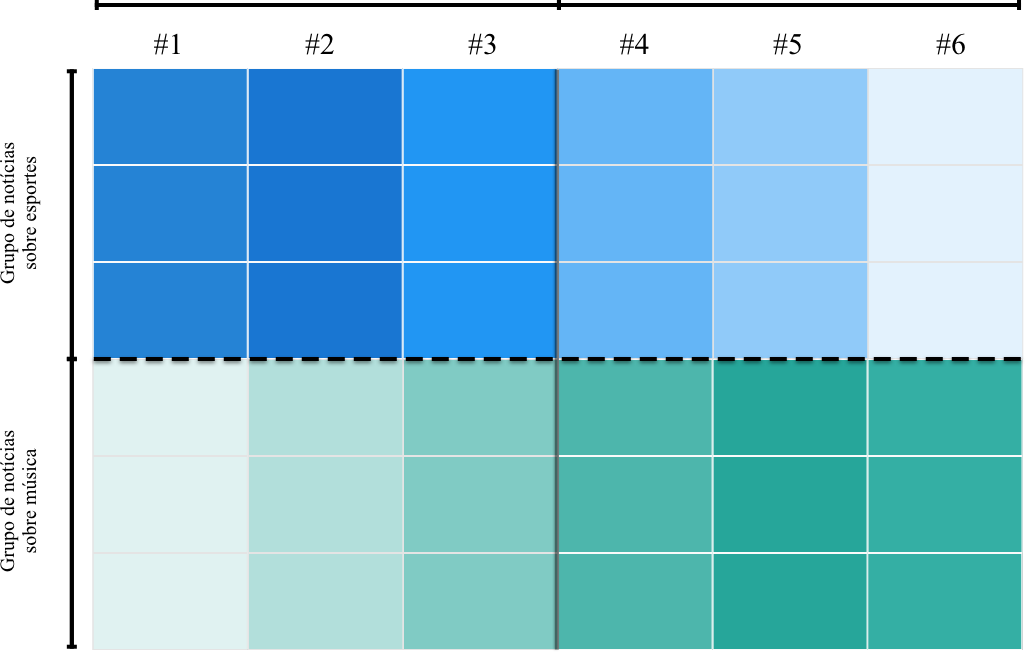
\includegraphics[width=3in]{img/sistema0.png}}\quad
%        \subfigure[ ]{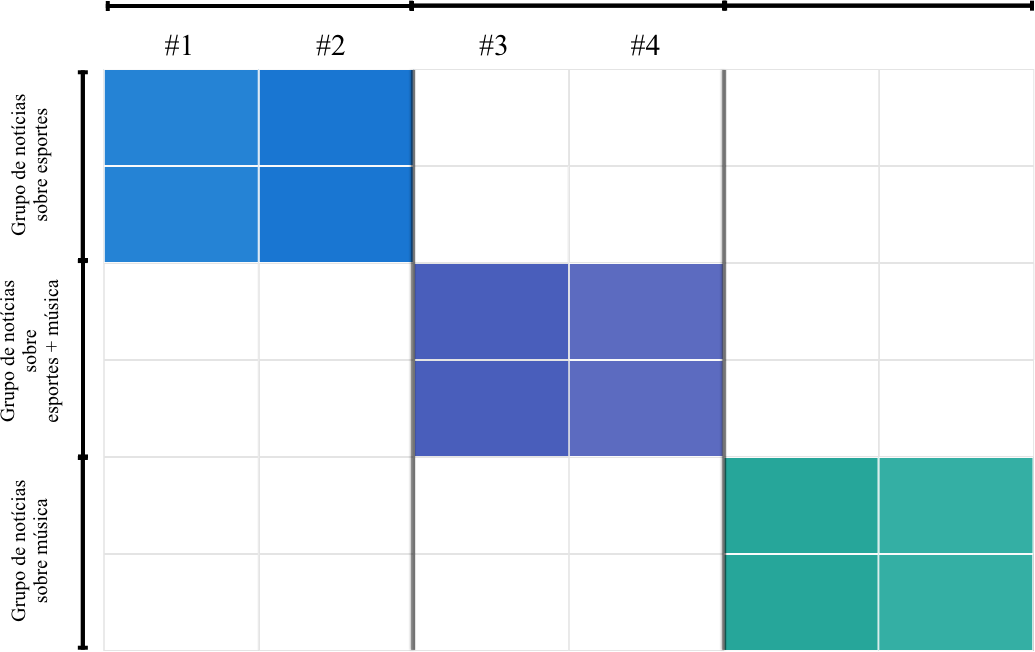
\includegraphics[width=3in]{img/sistema1.png}}
%       }
% \mbox{
%        \subfigure[ ]{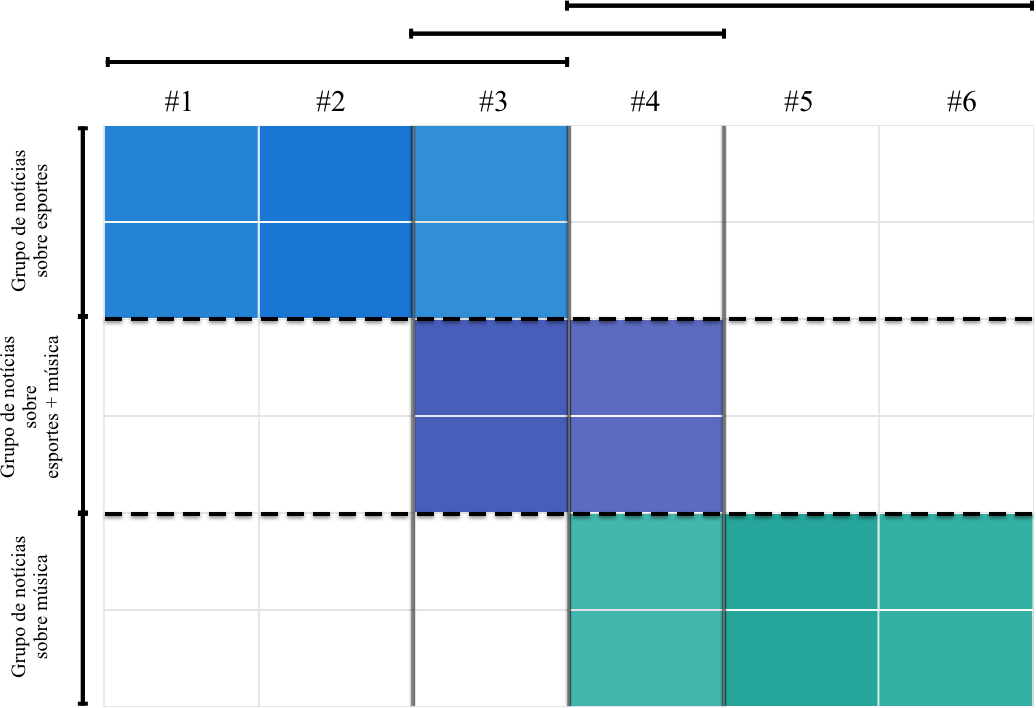
\includegraphics[width=3in]{img/sistema2.png}}\quad
%        \subfigure[ ]{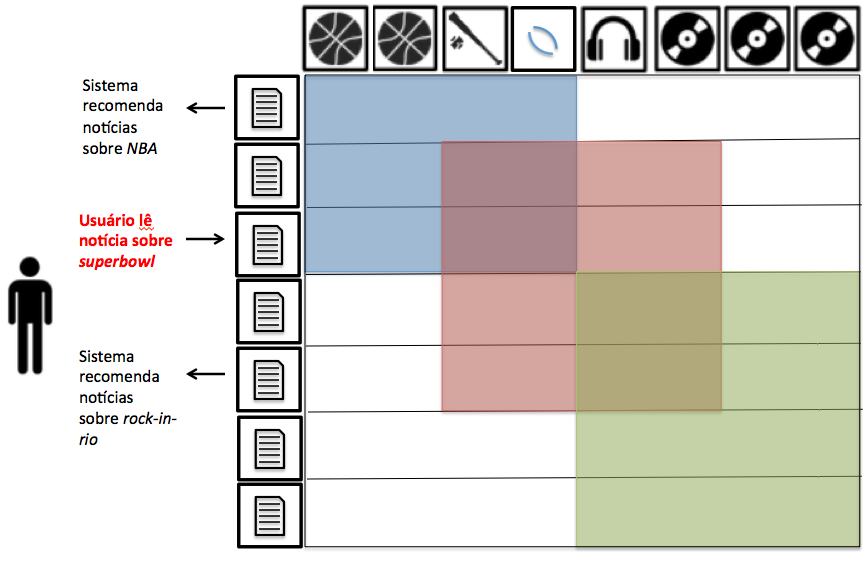
\includegraphics[width=3in]{img/sistema3.png}}
%       }
% %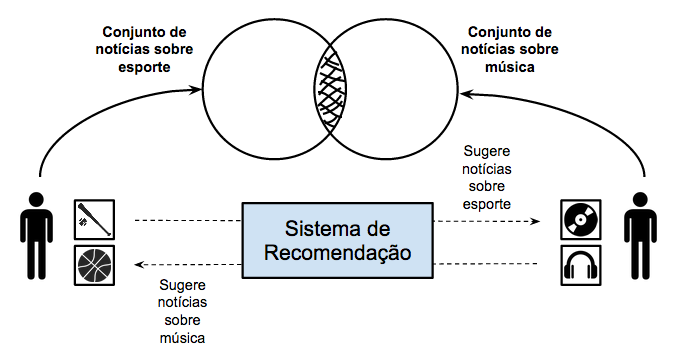
\includegraphics[width=120mm]{img/story.png}
% \caption{Representação do context de um Sistemas de Recomendação implementado a partir de análise de agrupamento com similaridade total (a) e similaridade parcial (b,c,d). Os grupos são diferenciados por cores.}
% \label{fig:story}
% \end{figure}

A associação da análise de coagrupamentos a mineração de textos é interessante por diferentes aspectos. A mineração de textos constitui-se como um problema no qual é preciso lidar com a necessidade de apresentação de resultados com boa interpretabilidade e com um espaço dos dados de alta-dimensionalidade. O primeiro problema é bem resolvido com a estratégia de coagrupamento pois os grupos de atributos que são gerados por ela podem revelar informação antes escondida nos dados \cite{Tjhi2009}, e que em um processo de agrupamento tradicional não poderiam ser, pelo menos diretamente, descobertas. Ainda segundo~\cite{Tjhi2009}, análise de coagrupamento pode apresentar bom desempenho em espaços de alta-dimensionalidade porque seu processo de agrupar atributos (características) pode ser visto com uma redução de dimensionalidade dinâmica para o espaço dos dados.

A despeito da capacidade intrínseca do processo de coagrupamento em lidar de forma diferenciada com o problema de alta-dimensionalidade, ainda se faz necessário notar que no contexto de mineração de dados, ocorre também o problema de esparsidade na representação dos dados. Assim, para implementar a estratégia de coagruapmento com alguma eficiência, é necessário adotar métodos que tenham a capacidade de lidar com esparsidade.

% tive dificuldade em justificar a escolha por fatoração de matrizes e de ligá-las à questão da esparsidade. Fiquei apenas com uma motivação. Acho que seria bom tentarmos justificar de forma mais contundente, se possível.
Dentre os diferentes métodos existentes na literatura referentes à implementação de análise de coagrupamento (\textcolor{blue}{citar artigos dos vários algoritmos que seguem outras linhas}), métodos que usam fatoração de matrizes não negativas~\cite{lee:nnmf00, lee99} têm sido vistos como uma boa alternativa a ser aplicada no contexto de mineração de textos~\cite{Xu2003, Shahnaz2006373, Yoo2010}.
%Lucas precisa olhar esses artigos direitinho para validar essas referências nesses lugares.

% ********************************************************************************************

\section{Definição do problema}

\textcolor{blue}{Eu estou entendendo que temos duas facetas do problema. Um deles é o mais obvio que é dar um jeito de descobrir os grupos com sobreposição e mostrar que é util para recomendação/textos etc. O outro é fazer a fatoração de matriz funcionar pra isso. Então acho que temos que dividir essa definição em duas partes: sobreposição nos cogrupos e fatoração funcionando nisso. Por isso dividi em duas partes, para ver se conseguimos mostrar isso.}

\subsection{Estruturas de coagrupamentos}

\textcolor{blue}{Então aqui entra a parte de mostrar as estruturas de cogrupos possíveis e destacar aquela que fatoração já resolve e depois a que não resolve e a que queremos resolver. Também contextualizar no problema de recomendação ou análise de textos. Figuras precisam entrar aqui para mostra as estruturas.}

\subsection{Coagrupamento e fatorização de matrizes}

A estratégia de coagrupamento pode ser apresentada como o processo de agrupamento simultâneo de linhas e colunas em uma matriz de dados, de forma que seja possível encontrar \textbf{cogrupos} nos quais um \textbf{grupo de objetos} (linhas) associado a um deles diz respeito a objetos que são similares entre si considerando um \textbf{grupo de atributos} (colunas), também associado ao cogrupo.

Com maior formalidade, dada uma matriz $X(N,M)$ \textcolor{green}{(prefiro dizer $X\in\mathds{R}^{N\times M}$)} em que $N$ é o número de linhas, $M$ o número de colunas e $x(m,n)$ é, geralmente, um número real representando a relação entre a linha $x_n$ \textcolor{green}{(linha $n$?)} e a coluna $y_m$ \textcolor{green}{(coluna $m$?)}, o problema de \textbf{coagrupamento} consiste em encontrar um conjunto $\mathcal{C}$ de submatrizes $G(I,J)$, onde $I=\{i_1, ..., i_r\}$ com $r \leq L$ e $J=\{j_1, ..., j_s\}$ com $s \leq C$, que maximize a similaridade entre os elementos $g\{i,j\}$. \textcolor{green}{(Quem é $L$ e $C$?)}

% \cite{Franca2010,Mirkin1996,Madeira2004}.

A \textbf{esparsidade} em uma matriz é caracterizada pela existência de poucos elementos diferentes de zero ({0}). Em termos gerais, a esparsidade de uma matriz pode ser medida como a proporção de elementos iguais a zero ($0$) que ela contém. Problemas de otimização que envolvem matrizes esparsas são caracterizados por apresentarem alta complexidade combinatorial para os quais algoritmos eficientes em matrizes não esparsas tem seu desempenho bastante prejudicado.

% Sparse Convex Optimization Methods for Machine Learning. Jaggi, Martin. Tese de doutorado. ETH Zürich, 2011, p. 192

% limitação teórica: não consegui encontrar nada que me desse base para dizer: isso trabalha bem (ou melhor que outras coisas) em dados esparsos. Achei algumas coisas usando fatorizacão para problemas de recomendação por filtro e tb achei para texto, mas ninguém esta falando de esparsidade (eu acho).

\textbf{Fatorar uma matriz} consiste em encontrar duas, ou mais, novas matrizes que ao serem multiplicadas, reconstroem a matriz original. Considere uma matriz $R(N,M)$ em que $N$ é o número de linhas, $M$ o número de colunas. A fatoração desta matriz em duas novas matrizes consiste em encontrar duas matrizes $U(N,K)$ e $D(M,K)$, tal que $ R = U \times D^t = \hat{R} $ \textcolor{green}{(Por que colocar $\hat{R}$? Só se for para dizer $ R \approx U \times D^t = \hat{R} $)}. Se $K$ é escolhido tal que seja menor do que $N$ e $M$, então é dito que $U$ e $D$ são representações compactas de $R$ \textcolor{green}{(Estranho, pois se $K=M-1$ parece que precisaremos de mais números e não haverá nenhuma compactação de dados)}. Se a matriz R, e as suas decomposições, são não negativas, tem-se o caso de  fatoração de matriz não-negativa.

% usar o artigo da nature para justificar a nao negativa??? Ou a justificativa vem do fato do nosso problema se encaixar nessa restrição. Essa restrição deixa o problema mais fácil de resolver?

O problema de coagrupamento pode ser modelado de tal forma que a fatoração de matriz é capaz de fornecer uma aproximação da organização em cogrupos presente no conjunto de dados sob análise.

Considere que o conjunto de dados sob análise é representado pela matriz $X(N,M)$, a fatoração dessa matriz em duas (ou mais) novas matrizes $U(N,K)$ e $D(M,K)$ significa que $K$ grupos de linhas foram descobertos, de acordo com $K$ grupos de colunas.

% Colocar a figura 2 do artigo do Yoo e Choi (referenciando, e claro).

Se três matriz são geradas na fatoração, $U(N,L)$, $S(L,K)$ e $D(M,K)$ , a interpretação pode incluir uma noção de pesos (matriz $S$) que relacionam grupos de linhas e grupos de colunas, e dimensões diferentes para as matrizes $U$ e $D$ podem ser admitidas de modo que o número de grupos de linhas pode ser diferente do número de grupo de colunas.

% Colocar a figura 3 do artigo do Yoo e Choi (referenciando, e claro).

\textcolor{blue}{Imagino que agora tem que entrar uma apresentação rápida do algoritmo novo.}

% ************************************************************************

% essa ilustração deveria ser deixada para um capítulo de coagraupamento

%O problema de Biclusterização pode ser ilustrado na Figura~\ref{fig:bicluster-exp}, onde se tem um conjunto de dados que possui objetos $x_1, x_2, x_3, x_4, x_5$ e $x_6$ que são representados pelos atributos $y_1, y_2, y_3, y_4, y_5$ e $y_6$, onde $N,M = 6$.
%Na Figura~\ref{fig:bicluster-exp} também estão ilustrados dois biclusters hipotéticos: o primeiro formado pelos objetos $x_5$ e $x_6$ e todos os atributos ($y_1, \dots, y_6$), representando um bicluster com \textit{modelo global}; e o segundo formado pelos objetos $x_2, x_3, x_4$ e $x_5$ e atributos $y_4, y_5$ e $y_6$, representando um bicluster com \textit{modelo local}, que leva em consideração apenas um subconjunto dos atributos.

%\begin{figure}[h]
%\centering
%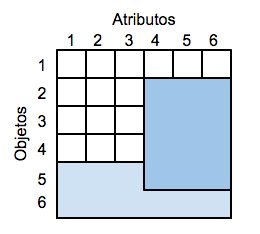
\includegraphics[width=80mm]{img/bicluster.png}
%\caption{Conjunto de dados com dois biclusters encontrados.}
%\label{fig:bicluster-exp}
%\end{figure}

% ************************************************************************

\section{Hipótese}

Fatoração de matrizes considerando a decomposição da matriz original em ... \textcolor{red}{como descrever em algo nível aqui??} ... possibilita a descoberta de cogrupos com sobreposição (de colunas); a partir das novas matrizes é possível extrair informação detalhada sobre a relação dos grupos de linhas em relação ao grupo de colunas que pode agregar valor à solução de um problema real de recomendação.

% Não estou certa de que devemos usar recomendação, talvez devessemos usar agrupamento de textos.

% ************************************************************************

\section{Objetivos}

O objetivo geral desse trabalho é o desenvolvimento de novas estratégias de coagrupamento baseadas em fatoração de matrizes, que sejam capazes de descobrir cogrupos com sobreposição em uma dimensão da matriz, isto é, ou sobreposição de colunas ou sobreposição de linhas, considerando uma matriz de valores reais positivos. Com a proposição dessas novas estratégias, este trabalho cobre uma lacuna presente na área de coagrupamento baseado em algoritmos de fatoração de matrizes.

%A clusterização, nesse contexto, deve atuar como estratégia de organização do conteúdo textual, agrupando itens em biclusters.Sendo que a partir da observação dos interesses do usuário e dos biclusters à que estes itens pertencem, é possível organizar a lista recomendação com itens desses biclusters que esse usuário ainda não interagiu.

Este trabalho tem como objetivos específicos a aplicação das novas estratégias em um contexto de aplicacão real, de forma a ilustrar que elas

Como objetivos específicos, este trabalho mostra que a aplicação das novas estratégias em ambientes controlados (matrizes de dados com cogrupos sintéticas) e em um contexto de aplicação real:

\begin{itemize}
    \item alcançam resultados tão bons quanto, ou melhores que, as estratégias correlatas que não permitem a sobreposição de dimensões nos cogrupos, quando medidas de qualidade quantitativas são consideradas;
    \item alcança resultados tão bons quanto, ou melhores que, estratégias de agrupamento quando análise de particionamento clássico e medidas de qualidade quantitativas são consideradas;
    \item é capaz de melhorar a interpretabilidade qualitativa dos resultados quando comparada aos resultaods fornecidos por estratégias de agrupamento clássico.
\end{itemize}

%Assim, com o intuito de melhor definir o contexto de estudo deste trabalho, foram estabelecidos os seguintes objetivos específicos:

%\begin{itemize}

% se nomearmos as estratégias podemos chamá-las pelo nome aqui

%\item apresentação de uma derivação formal, incluindo uma prova de convergência, para a estratégia de coagrupamentos usando fatoração de matrizes não-negativas capaz de lidar com matrizes binárias;

%\item apresentação de uma derivação formal para a estratégia de coagrupamento usando fatoração de matrizes não negativas capaz de lidar com matrizes de valores reais positivos;

%\item apresentar experimentos que ilustram a eficácia das estratégias propostas considerando dados sintéticos e dados reais, mostrando inclusive o potencial de descoberta de informações de valor diferenciado para as aplicações em teste (recomendação baseada em conteúdo textual).


% \item Levantamento do referencial teórico de SRs.
% \begin{itemize}
%  \item Levantamento do estado da arte sobre o uso de Aprendizado de Máquina na implementação de SRs baseados em conteúdo textual.
% \end{itemize}
% \item Levantamento do referencial teórico sobre Biclusterização e Mineração de Texto.
% \item Construção de um corpus de itens textuais e um conjunto de dados de recomendação.
% \item Implementação e teste dos algoritmos de Biclusterização sobre o corpus construído.
% \item Modelagem do problema de recomendação baseado em conteúdo considerando a existência de biclusters de itens.
% \item Análise da viabilidade da modelagem proposta frente ao conjunto de dados de recomendação e frente a análise qualitativa do alcance da serendipidade.
 % \item estudo das técnicas de essemble aplicadas a texto

%\end{itemize}

% ************************************************************************

\section{Metodologia}

A análise exploratória da literatura especilizada foi escolhida como estratégia para a aquisição de conhecimento sobre a área de coagrupamento e fatoração de Matrizes aplicada à coagrupamento.

\textcolor{blue}{E não estou conseguindo encontrar uma forma de descrever a parte referente à concepção das estratégias propostas e também não sei como definir as estratégias referente às derivações.}

%Já para o levantamento do estado da arte em SRs baseados em conteúdo textual e sobre a aplicação de técnicas de Aprendizado de Máquina, mais especificamente clusterização, em SRs baseados em conteúdo textual, optou-se por aplicar a técnica de construção de revisões sistemáticas. A Revisão Sistemática (RS) é um tipo de revisão bibliográfica documentada, na qual cada passo da pesquisa é registrado seguindo critérios rigorosos, e portanto permitindo facilmente a auditoria e reprodução da pesquisa. Segundo \citeonline{Kitchenham2004}, a RS é um meio de avaliar, identificar e interpretar todas as pesquisas relevantes disponíveis em uma determinada área com base em questões de pesquisa. A RS que relaciona Aprendizado de Máquina e SRs se faz útil uma vez que a aplicação de Biclusterização como estratégia de resolução do problema é o núcleo deste projeto. Apesar de estar sendo realizada uma RS, neste documento optou-se por apresentar uma revisão bibliográfica no formato simples, isto é, sem os processos detalhados em \citeonline{Kitchenham2004}, visto que a construção da RS ainda esta em andamento.

A fim de permitir a validação das estratégias propostas e, portanto, a verificação da  hipótese, fez-se necessário a definição de: (a) um ambiente de teste controlado, representado por uma coleção de conjuntos de dados sintéticos, contendo cada um dos conjuntos situações diferentes referentes às estrutura de coagrupamento e variações em relação à esparsidade;  (b) um contexto para realização de uma prova de conceito, no qual um conjunto de dados real foi construído.

Para a prova de conceito foi escolhido usar o conteúdo referente à notícias publicadas no portal iG\footnote{http://ig.com.br/}.
Trata-se de um portal de notícias brasileiro muito conhecido, com um volume de notícias bastante grande e com notícias categorizadas em canais, que representam os assuntos dessas notícias. Essas características conferem liberdade para a configuração de experimentos de diferentes naturezas, como experimentos considerando determinadas categorias de notícias, tipos de notícias ou datas de publicação das notícias.

A partir do conteúdo de notícias do portal iG foi construído um corpus de dados textuais, categorizados de acordo com as categorias já usadas no referido portal.
Todo o conteúdo do corpus passou por rotinas de pré-processamento comuns na área de Mineração de Texto: \textit{tokenização}, filtragem de \textit{stopwords}, remoção de sufixos (\textit{stemming}), representação da relação ``termos $\times$ documentos'' usando estratégias de frequência de termos, como TF-IDF e \textit{n-grams}.

%Leia com muito cuidado e veja se faz sentido. MUITO CUIDADO.ALTERE O QUE FOR NECESSÄRIOS TAMBÉM COM MUITO CUIDADO.
%Também, o portal iG possui informações históricas e anônimas referentes ao registro de navegação de usuários.
%Esse registro permite a construção de um conjunto de dados de preferências, que pode ser usado para realização de \textit{testes offline} entre recomendações oferecidas pela abordagem proposta e a navegação real realizada por um conjunto de usuários, utilizando métricas como precisão, revocação \cite{Jannach2011} e comparação com recomendações geradas por filtro colaborativo.

Os resultados da aplicação das estratégias de coagrupamento foram validados utilizando técnicas de avaliação interna, para a verificação da consistência dos biclusters encontrados \cite{Santamaria2007}, e externas \cite{Hochreiter2010}, avaliando o quanto os biclusters encontrados estão em consenso com as classes de notícias \cite{Hochreiter2010}.

\textcolor{blue}{Então precisaremos dizer aqui como fizemos a avaliação qualitativa.}

% essa parte aqui ficou bem frágil.
% Os algoritmos de análise de texto via Biclusterização deverão ser validados antes de serem aplicados ao corpus criado.
% Para isso, conjuntos de dados de referência para Biclusterização e para clusterização de texto deverão ser usados.
% Uma vez alcançada a análise dos textos via Biclusterização, o modelo de uso dos biclusters em um contexto de recomendação deverá ser delineado e analisado.
% A análise deverá estar baseando tanto em comparações com o conjunto de dados de recomendação do portal iG quando por análise qualitativa do alcance da serendipidade.

%Para conhecer a área de Sistemas de Recomendação foi realizado um levantamento do referencial teórico através da análise exploratória de livros e artigos do tipo revisão bibliográfica \cite{Adomavicius2005,Lops2011,Ricci2011,Ricci22011,Jannach2011,Burke2002}, o que permitiu, em seguida, o aprofundamento na área de SRs.
%Para o aprofundamento na área de SRs, foi realizada uma Revisão Sistemática de SRs baseados em conteúdo textual.
%Também foi realizado um levantamento do referencial teórico, através da análise exploratória de livros e artigos do tipo revisão bibliográfica, na área de Mineração de Dados \cite{Berry2010,Feldman2006,Miner2012,Hotho2005,Weiss2010}, para que fosse possível realizar a análise e estruturação do conteúdo não-estruturado, presentes nas notícias.

%Isso tudo tem que vir no capitulo da propsota, como eu disse, aqui é não é um momento de relatar atividades realizadas.
% Sendo assim, com a extração das notícias do portal iG\footnote{http://ig.com.br/} através de um \textit{web crawler} utilizando a linguagem python\footnote{https://www.python.org/}, foi possível construir o corpus iG (Subseção~\ref{subsec:corpusig}) de notícias.
%As notícias foram capturadas a partir de uma página de início, fornecida para o \textit{web crawler}, que era selecionada a fim de equalizar a distribuição de notícias por ano e por assunto. Este trabalho também conta com uma base de cliques em notícias (Subseção~\ref{subsec:basecliquesig}), doada pelo portal de notícias iG.

%idem
%Para aplicação dos algoritmos de Biclusterização, foi realizado um levantamento do referencial teórico, através da análise exploratória de livros, artigos do tipo revisão bibliográfica e artigos que se referem à criação dos algoritmos \cite{Cheng2000,Tanay2005,Madeira2004,Santamaria2007,Kluger2003,Prelic2006}.

%Para gerar conhecimento do corpus iG, serão aplicados algoritmos de Biclusterização que estão sendo implementados\footnote{https://github.com/lucasbrunialti/biclustering-experiments} nos textos das notícias processados e representados por diversas estratégias (TF-IDF, TF-IDF normalizado e n-gramas). Assim, será possível avaliar o resultado dos algoritmos utilizando a base de dados de cliques iG.

% ************************************************************************

\section{Organização do documento}

Esta dissertação é composta por \textcolor{red}{XXX} capítulos incluindo esta introdução. Os demais capítulos estão divididos em duas partes: a primeira é dedicada a explorar a estratégia  de coagrupamento implementada com algoritmos baseadas em fatoração de matrizes; a segunda é dedicada a explorar o contexto de sistemas de recomendação baseados em conteúdo textual a partir da aplicação das estratégias de coagrupamento estudadas.

No capítulo~\ref{ch:conceitos} são apresentados os principais conceitos referentes à área de coagrupamentos. \textcolor{blue}{Especificar mais detalhes ... ... }

Estratégias de fatorização de matrizes aplicadas à coagrupamentos são discutidas no capítulo .....

A principal contribuição deste trabalho, as estratégias ... ...., é apresentada em detalhes no capítulo ... ...

% e então organizar a segunda parte

% ************************************************************
% ************************************************************
% ************************************************************

\chapter{Conceitos Fundamentais}
\label{ch:conceitos}

\textcolor{red}{Esses conceitos fundamentais ainda vem na qualificação. Não estão ajustados ao que está sendo discutido agora, para a fase final.}

Técnicas e algoritmos de Biclusterização são usados, principalmente, no contexto de expressão genética. No entanto, algoritmos de Biclusterização se fazem úteis quando se deseja encontrar \textit{modelos locais}. Ou seja, enquanto algoritmos de clusterização têm o intuito de encontrar \textit{modelos globais}, que geram grupos de dados levando em consideração todas as características, algoritmos de Biclusterização geram grupos de dados em que as características tem alta correlação \cite{Franca2010,Madeira2004}.

% lembrar de inserir informação sobre two-way clustering e FCA - conforme informação passada pelo Fabrício no email.

Para a descrição do problema formal de Biclusterização usa-se a seguinte definição \cite{Madeira2004}: seja uma matriz $A$, de dimensão $N \times M$, um conjunto de linhas $X = \{ x_1, \dots, x_n, \dots, x_N \}$ \textcolor{green}{(aqui deveria ser $X=\{1,2,\ldots,n,\ldots,N\}$)} e um conjunto de colunas $Y = \{ y_1, \dots, y_m, \dots, y_M \}$ \textcolor{green}{(mesmo comentário anterior)}, em que $a_{nm}$ geralmente é um número real e representa a relação entre a linha $x_n$ e a coluna $y_m$; o problema de Biclusterização é encontrar biclusters, que são submatrizes de $A$, denotados por $A_{IJ}$, em que $I \subseteq X$ e $J \subseteq Y$. Assim, o bicluster $A_{IJ}$ é um grupo dos objetos em $I$, perante as características com alta correlação $J$.

\section{Tipos de cogrupos }
\label{sec:tiposbic}

Como a definição de bicluster não inclui uma prévia estrutura da matriz $A$ e dos biclusters $A_{IJ}$, diversos algoritmos propostos na literatura diferem quanto ao tipo de bicluster que são capazes de encontrar.
Uma taxonomia dos tipos de biclusters é proposta por \citeonline{Madeira2004}:
 \begin{itemize}
  \item \textit{Biclusters com valores constantes}, se trata de biclusters em que todos os valores de $A_{IJ}$ são constantes: $a_{ij} = \mu, \forall i,j \in I,J$, \textcolor{green}{(aqui o valor de $\mu$ não deveria ser indexado por $IJ$, isto é, $\mu_{IJ}$? O mesmo para os outros $\mu$ que aparecem abaixo.)} onde $\mu$ é um valor constante dentro de $A_{IJ}$. Porém, em conjuntos de dados reais, esses biclusters estão presentes com algum tipo de ruído $\mu + \eta_{ij}$, onde $\eta_{ij}$ é o ruído associado com os valores de $\mu$ e $a_{ij}$ \cite{Madeira2004}.
  \item \textit{Biclusters com valores constantes nas linhas ou colunas}, se trata de biclusters com valores constantes nas linhas: $a_{ij} = \mu + \alpha_i, \forall i,j \in I,J$ ou $a_{ij} = \mu \cdot \alpha_i, \forall i,j \in I,J$, onde $\alpha_i$ é um fator aditivo ou multiplicativo para cada linha; ou ainda biclusters com valores constantes nas colunas: $a_{ij} = \mu + \beta_j, \forall i,j \in I,J$ ou $a_{ij} = \mu \cdot \beta_j, \forall i,j \in I,J$, onde $\beta_j$ é um fator aditivo ou multiplicativo para cada coluna \cite{Madeira2004}.
  \item \textit{Biclusters com valores coerentes}, em que são considerados valores próximos entre si (coerentes) para definição de um bicluster: $a_{ij} = \mu + \alpha_i + \beta_j, \forall i,j \in I,J$, ou $a_{ij} = \mu' \cdot \alpha_i' \cdot \beta_j', \forall i,j \in I,J$, sendo que se $\mu = \log \mu'\implies \alpha_i = \alpha_i', \beta_j = \beta_j'$ \cite{Madeira2004}.
  \item \textit{Biclusters com evoluções coerentes} têm seus valores com evoluções coerentes, por exemplo, um bicluster com $a_{i4} \leq a_{i3} \leq a_{i2} \leq a_{i1}$ tem valores com evolução coerente na coluna \cite{Madeira2004} \textcolor{green}{(estranho considerar a ordem das colunas ou das linhas, já que na maioria dos problemas pode ser bem arbitrário.)}. Seus valores podem ser gerados por uma função geradora de valores com evolução coerente $a_{ij} = g(a_{ij}), \forall i,j \in I,J$, sendo $g(\cdot)$ não linear e não constante, para que o tipo de bicluster não seja classificado nos casos anteriores. \textcolor{green}{(Muito estranho $a=g(a)$, pois $g()$ deveria ser a identidade)}
 \end{itemize}

Os biclusters também diferem quanto as suas estruturas. Cada algoritmo usado para implementar Biclusterização faz uma suposição da estrutura de biclusters que é capaz de encontrar.
A Figura~\ref{fig:bicstruct} sumariza as diferentes estruturas de biclusters, com as linhas e colunas ordenadas para permitir a visualização dos biclusters por meio do mapa de calor dos valores de $A$, sendo os biclusters $A_{IJ}$ representados por cores sólidas e o fundo da matriz ruído.

% Os tipos de estruturas são: Bicluster único, tem apenas um bicluster na matriz (Figura~\ref{fig:bicstruct-a}); Bicluster com linhas e colunas exclusivas

% Para melhorar esse figura, deixe na figura apenas as letras (a), (b) etc e faça uma legenda. Acho que você pode usar \caption*{} em cima do \caption{} para fazer a legenda. Ou crie um parágrafo para explicar as letras na figura. Acho que aaté fica mais simpático fazer um parágrafo, pois pode explicar com mais cuidado.

% \begin{figure}[h]
%     % \captionsetup[subfigure]{labelformat=simple}
%     \centering
%     \begin{subfigure}[b]{0.3\textwidth}
%             
\includegraphics[width=30mm]{img/a-bic-struct.png}
%             \caption{Bicluster único}
%             \label{fig:bicstruct-a}
%     \end{subfigure}
%     ~
%     \centering
%     \begin{subfigure}[b]{0.3\textwidth}
%             
\includegraphics[width=30mm]{img/b-bic-struct.png}
%             \caption{Biclusters com linhas e colunas exclusivas}
%             \label{fig:bicstruct-b}
%     \end{subfigure}
%     ~
%     \centering
%     \begin{subfigure}[b]{0.3\textwidth}
%             
\includegraphics[width=30mm]{img/c-bic-struct.png}
%             \caption{Biclusters com estrutura de tabuleiro de xadrez}
%             \label{fig:bicstruct-c}
%     \end{subfigure}
%     ~
%     \centering
%     \begin{subfigure}[b]{0.3\textwidth}
%             
\includegraphics[width=30mm]{img/d-bic-struct.png}
%             \caption{Biclusters com linhas exclusivas}
%             \label{fig:bicstruct-d}
%     \end{subfigure}
%     ~
%     \centering
%     \begin{subfigure}[b]{0.3\textwidth}
%             
\includegraphics[width=30mm]{img/e-bic-struct.png}
%             \caption{Biclusters com colunas exclusivas}
%             \label{fig:bicstruct-e}
%     \end{subfigure}
%     ~
%     \centering
%     \begin{subfigure}[b]{0.3\textwidth}
%             
\includegraphics[width=30mm]{img/f-bic-struct.png}
%             \caption{Biclusters sem sobreposição com estrutura em árvore}
%             \label{fig:bicstruct-f}
%     \end{subfigure}
%     ~
%     \centering
%     \begin{subfigure}[b]{0.3\textwidth}
%             
\includegraphics[width=30mm]{img/g-bic-struct.png}
%             \caption{Biclusters sem sobreposição e não exclusivos}
%             \label{fig:bicstruct-g}
%     \end{subfigure}
%     ~
%     \centering
%     \begin{subfigure}[b]{0.3\textwidth}
%             
\includegraphics[width=30mm]{img/h-bic-struct.png}
%             \caption{Biclusters com sobreposição com estrutura hierarquica}
%             \label{fig:bicstruct-h}
%     \end{subfigure}
%     ~
%     \centering
%     \begin{subfigure}[b]{0.3\textwidth}
%             
\includegraphics[width=30mm]{img/i-bic-struct.png}
%             \caption{Biclusters com sobreposição arbitrariamente posicionados}
%             \label{fig:bicstruct-i}
%     \end{subfigure}
%     \caption{Diferentes estruturas de biclusters, quadrados e retângulos com cores sólidas representam biclusters e o fundo representa ruído.}% (Adaptado de \cite{Madeira2004})}
%     \label{fig:bicstruct}
% \end{figure}

\section{Algoritmos para Biclusterização}

Diversos algoritmos para encontrar biclusters, de diferentes tipos e estruturas, foram propostos na literatura \cite{Tanay2005,Madeira2004}.

Um dos algoritmos de Biclusterização mais comum e simples. que encontra biclusters com valores coerentes, em estrutura com sobreposição e arbitrariamente posicionados, é o \textit{Coupled Two-way Clustering} (CTWC) \cite{Getz2000}. O algoritmo CTWC é capaz de encontrar biclusters através da clusterização de objetos e atributos (linhas e colunas), separadamente.
O algoritmo de clusterização usado por \citeonline{Getz2000} foi o \textit{Superparamagnetic Clustering} (SPC), o qual é capaz de determinar o número de clusters automaticamente, e com uma estratégia de clusterização hierárquica \textit{top-down} é capaz de gerar clusters estáveis \cite{Getz2000}.
O SPC tem como entrada uma matriz de similaridade e um parâmetro temperatura, que controla o quão estáveis serão os clusters que o algoritmo gerará.
Assim, o CTWC encontra clusters estáveis de linhas e colunas através do SPC, e iterativamente executa o SPC nos clusters de linhas e colunas encontrados, mantendo na memória um par do subconjunto de linhas e do subconjunto de colunas (biclusters), assim como os clusters estáveis de linhas e colunas, separadamente.
% O algoritmo se inicia com dois subconjuntos: um para exemplos (linhas) $I = \{ X \}$ e um para características (colunas) $J = \{ Y \}$, então, através do algoritmo de SPC

Já o algoritmo de \citeonline{Cheng2000} é capaz de encontrar o mesmo tipo de bicluster que o algoritmo CTWC, porém usando uma estratégia gulosa: biclusters com valores coerentes e estrutura com sobreposição e arbitrariamente posicionados. Este algoritmo esta sendo objeto de estudo desse projeto de mestrado para aplicação em dados textuais e por isso segue aqui descrito em mais detalhes.
Nesse algoritmo, para encontrar biclusters, ou $\delta$-biclusters, na matriz $A$, os autores definem o \textit{Resíduo Quadrático Médio} (RQM):
\begin{equation}
\begin{split}
    H_{IJ} = \frac{1}{|I||J|} \displaystyle\sum_{i,j \in I,J} (a_{ij} - a_{iJ} - a_{Ij} + a_{IJ})^2 \\
    H_{iJ} = \frac{1}{|J|} \displaystyle\sum_{j \in J} (a_{ij} - a_{iJ} - a_{Ij} + a_{IJ})^2 \\
    H_{Ij} = \frac{1}{|I|} \displaystyle\sum_{i \in I} (a_{ij} - a_{iJ} - a_{Ij} + a_{IJ})^2   \nonumber
\end{split}
\end{equation}
em que
\begin{equation}
    a_{iJ} = \frac{1}{|J|} \displaystyle\sum_{j \in J} a_{ij},\quad a_{Ij} = \frac{1}{|I|} \displaystyle\sum_{i \in I} a_{ij},\quad a_{IJ} = \frac{1}{|I||J|} \displaystyle\sum_{i,j \in I,J} a_{ij}   \nonumber
\end{equation}
onde $H_{IJ}$ é o RQM de uma submatriz $A_{IJ}$, $H_{iJ}$ o RQM da linha $i$, $H_{Ij}$ o RQM da coluna $j$, $a_{iJ}$ a média dos valores da linha $i$, $a_{Ij}$ a média dos valores da coluna $j$ e $a_{IJ}$ a média dos valores da submatriz $A_{IJ}$, definida pelos subconjuntos $I$ e $J$.

Então, um bicluster perfeito $A_{IJ}$ teria o RQM $H_{IJ} = 0$, pois $a_{ij} = a_{ij}, \forall i,j \in I,J$, \textcolor{green}{($a_{ij}=a_{ij}$, hein? não seria $a_{ij}=a_{iJ}+a_{Ij}-a_{IJ}$?)} fazendo $a_{iJ} = a_{Ij} = a_{IJ}$. No entanto, se apenas minizar o RQM, um bicluster com apenas um elemento seria perfeito, o que pode não refletir a realidade. Além disso, em conjunto de dados reais existe ruído, podendo esconder o bicluster perfeito.

Para encontrar biclusters, ou $\delta$-biclusters, \citeonline{Cheng2000} usam uma estratégia gulosa que retira linhas e colunas, visando a minimização do RQM, respeitando um parâmetro $\delta$, que é calibrado pelo usuário. Então, um bicluster é encontrado quando o RQM de uma submatriz $A_{IJ}$ é $H_{IJ} \leq \delta$, para algum $\delta \geq 0$. As etapas de remoções de elementos da matriz são apresentadas nos algoritmos 1 e 2.

% \begin{algorithm}[H]
% \label{algo:cc1}
%  \KwData{$A, I, J, \delta$}
%  \KwResult{$I,J$ onde $H_{IJ} \leq \delta$}
%  \While{$H_{IJ} > \delta$}{
%   encontre a linha $l_{max} = \operatorname*{arg\,max}_{i \in I} H_{iJ}$\;
%   encontre a coluna $c_{max} = \operatorname*{arg\,max}_{j \in J} H_{Ij}$\;
%   \eIf{$l_{max} > c_{max}$}{
%    remova $l_{max}$ do subconjunto $I$\;
%    }{
%    remova $c_{max}$ do subconjunto $J$\;
%   }
%  }
%  \caption{Remove uma linha ou coluna a cada iteração.}
% \end{algorithm}

% \begin{algorithm}[H]
% \label{algo:cc2}
%  \KwIn{$A, I, J, \delta, \alpha$}
%  \KwOut{$I,J$ onde $H_{IJ} \leq \delta$}
%  \While{$H_{IJ} > \delta$}{
%   remova $i \in I$ onde $H_{iJ} > \alpha \cdot H_{IJ}$\;
%   remova $j \in J$ onde $H_{Ij} > \alpha \cdot H_{IJ}$\;
%   encontre a coluna $c_{max} = \operatorname*{arg\,max}_{j \in J} H_{Ij}$\;
%   \If{não houve nenhuma remoção}{
%    chame o algoritmo 1
%   }
%  }
%  \caption{Remove múltiplas linhas e colunas de $A$ a cada iteração.}
% \end{algorithm}

O algoritmo 2 é usado para acelerar o processo de busca de um $\delta$-bicluster, convergindo mais rapidamente para uma solução quanto maior for o parâmetro $\alpha$, em que $\alpha \geq 0$. Ainda, para amenização do problema de encontrar $\delta$-biclusters perfeitos com apenas um elemento, ou poucos elemento, é utilizado o algoritmo 3, que adiciona nós sem aumentar o RQM do bicluster.

% deu problema nessas referencias cruzadas, verifique.

% \begin{algorithm}[h]
% \label{algo:cc3}
%  \KwIn{$A, I, J$}
%  \KwOut{$I',J'$ onde $H_{I'J'} \leq H_{IJ}$}
%  \While{$H_{IJ} > \delta$}{
%   compute $a_{iJ}$ e $a_{Ij}$ para todo $i,j$ e $H_{IJ}$\;
%   remova $j \notin J$ onde $\frac{1}{|I|} \sum_{j \in J} (a_{ij} - a_{iJ} - a_{Ij} + a_{IJ})^2 \leq H_{IJ}$\;
%   recompute $a_{iJ}$ e $H_{IJ}$\;
%   remova $i \notin I$ onde $\frac{1}{|J|} \sum_{i \in I} (a_{ij} - a_{iJ} - a_{Ij} + a_{IJ})^2 \leq H_{IJ}$\;
%   \If{não houve nenhuma adição}{
%    $I' \longleftarrow I$\;
%    $J' \longleftarrow J$\;
%   }
%  }
%  \caption{Adiciona linhas e colunas de $A_{IJ}$ a cada iteração.}
% \end{algorithm}

Por fim, o algoritmo 4 é a consolidação dos algoritmos 3, 2 e 1 e a iteração para encontrar $k$ $\delta$-biclusters, um a um, sendo $k$ fornecido pelo usuário.

% \begin{algorithm}[h]
% \label{algo:cc4}
%  \KwIn{$A, k, \delta, \alpha$}
%  \KwOut{$k$ $\delta$-biclusters}
%  $A' \leftarrow A$\;
%  \For{$1$ \KwTo $k$}{
%    $B \leftarrow$ algoritmo 2 com $A', \delta, \alpha$\;
%    $C \leftarrow$ algoritmo 1 com $B, \delta$\;
%    $D \leftarrow$ algoritmo 3 com $A, C$\;
%    reporte $D$ como uma solução\;
%    adicione ruído em $A'$ para a submatriz $D$\;
%  }
%  \caption{Algoritmo Cheng \& Church, encontra $k$ $\delta$-biclusters.}
% \end{algorithm}

% Algoritmo Spectral (?)

Além dos algoritmos apresentados, existem outros algoritmos que são capazes de encontrar outros tipos de biclusters (Seção~\ref{sec:tiposbic}), além de serem recentes \cite{Franca20102,Yang2013,Hochreiter2010,Cabanes2012}, mostrando que ainda há interesse na área de pesquisa de Biclusterização.

 \section{Avaliação de Biclusterização}

Para determinar parâmetros, descobrir a qualidade e/ou estabilidade dos biclusters encontrados por algoritmos, é necessário estabelecer métricas de avaliação. Existem duas maneiras de avaliar biclusters \cite{Hochreiter2010}: \textit{interna}, usa os dados dos resultados dos algoritmos, juntamente com métricas de qualidade e/ou estabilidade, para avaliar as soluções geradas; \textit{externa}, utiliza os dados reais das soluções de biclusters de um conjunto de dados, usando estratégias para comparação, obtendo assim, maior confiança nas soluções.

A avaliação interna pode não ser tão precisa quanto a avaliação externa, porém é útil para descobrir parâmetros ótimos. Apesar de \citeonline{Prelic2006} sugerirem não usar avaliações internas, por não estar claro como estender noções de separação e homogeneidade, \citeonline{Santamaria2007} descreveu métricas de consistência para verificar se um bicluster é consistente com a sua definição, seja aditiva, multiplicativa e/ou constante, fazendo uma comparação dos elementos do bicluster:
\begin{equation}
\begin{split}
C_l(A_{IJ}) = \frac{1}{|I|} \displaystyle\sum_{i = 1}^{|I| - 1} \displaystyle\sum_{j = i + 1}^{|I|} \sqrt{ \displaystyle\sum_{k = 1}^{|J|} (a_{ik} - a_{jk})^2 } \\
C_c(A_{IJ}) = \frac{1}{|J|} \displaystyle\sum_{i = 1}^{|J| - 1} \displaystyle\sum_{j = i + 1}^{|J|} \sqrt{ \displaystyle\sum_{k = 1}^{|I|} (a_{ki} - a_{kj})^2 }    \nonumber
\end{split}
\end{equation}
em que $C_l(A_{IJ})$ é o índice de consistência das linhas do bicluster $A_{IJ}$ e $C_c(A_{IJ})$ é o índice de consistência das colunas do bicluster $A_{IJ}$. Ainda, a consistência do bicluster inteiro $C$ pode ser definida pela média:
\begin{equation}
C(A_{IJ}) = \frac{|I| \cdot C_l + |J| \cdot C_c}{|I| + |J|}   \nonumber
\end{equation}

Uma das métricas externas que são usadas para comparar biclusters encontrados com biclusters reais em um conjunto de dados, é a métrica \textit{concensus score} \cite{Hochreiter2010}. Essa métrica calcula a maximização das similaridades entre biclusters encontrados e reais, usando o \textit{índice de Jaccard} como medida de similaridade e o algoritmo Húngaro para solucionar o problema de maximização. A saída da avaliação é um $\textit{score} \in [0,1]$, em que $0$ significa que os biclusters comparados são totalmente diferentes, e $1$ o inverso.

% ********************************************************************************
% ********************************************************************************
% ********************************************************************************
% ********************************************************************************

\chapter{Fatoração de matrizes não-negativas para coagrupamento}
\label{ch:fatoracao}

% TODO: resgatar fatoração de matrizes tradicionais
% Acredito que não precisamos de mais do que já foi dito na introdução sobre fatoração de matrizes. A menos que se deseje explicar como se implementar a fataração. Então por enquanto estou suprimindo este passo.

% \section{Non-negative Matrix Factorization}

Fatoração de matrizes não-negativas (\textit{Non-negative Matrix Factorization} - NMF) foi estudada como um método para análise de dados capaz de extrair conhecimento sobre um objeto a partir do estudo de suas partes \cite{lee99}, como um contraponto a métodos mais populares como Análise de Componentes Principais (\textit{Principal Component Analysis - PCA}) e Quantização Vetorial, porém, considerando a fatoração matrizes positivas ou negativas.
\citeonline{lee99} apresentam tal abordagem a partir de sua aplicação no aprendizado de características de faces (em dados do tipo imagem) e na análise de características semânticas de textos.
A análise de textos também foi usada como aplicação na ilustração da aplicação de fatorização de matrizes por~\citeonline{Ho2008} que segue a ideia de aprendizado de partes, por \citeonline{Kuang2014} que aplica fatoração de matrizes não-negativas sobre um problema formulado como análise de agrupamento (clustering), e por~\citeonline{Long2005, Ding06, Yoo2010}, que formulam o problema como coagrupamento (coclustering).
Ainda, outros contextos são submetidos à análise sob a formulação de problemas de coagrupamento, sendo alguns exemplos a clusterização de genes e análise de microarry em bioinformática~\cite{Kluger2003} e a filtragem colaborativa em sistemas de recomendação~\cite{SalMnih08}.
Na aplicação de NMF em filtragem colaborativa em sistemas de recomendação, destaca-se o modelo baseado em NMF de~\citeonline{Koren09} para predição de preferências de usuários por filmes, que ganhou em primeiro lugar o Prêmio Netflix (\textit{Netflix Prize})\footnote{http://www.netflixprize.com/}.

A adequação da fatoração de matrizes para tarefas modeladas como agrupamento ou coagrupamento ocorre porque muitas das representações usadas em aplicações nessas áreas se apresentam como uma relação entre pares de elementos pertencentes a conjuntos finitos, como apresentado em \cite{Long2005}. Por exemplo, na resolução da tarefa de agrupamento de documentos, em mineração de textos, usa-se, comumente, dois conjuntos finitos, documentos e palavras, sendo que a relação entre eles é representada pela ocorrência de uma determinada palavra em um determinado documento. Note ainda que a relação expressa entre os elementos, como no contexto de palavras e documentos, apresenta-se como uma matriz de dados positiva, característica que ilustra a aplicabilidade de NMF.

Formalmente, algoritmos de coagrupamento baseados em NMF têm como entrada uma matriz de dados $X \in \mathbb{R}^{n \times m}_{+}$, contendo números reais positivos com $n$ linhas e $m$ colunas.
Esta matriz é formada por um conjunto de vetores de linhas $\mathcal{N} = \{ \mathbf{x}_{1 \cdot}, \dots, \mathbf{x}_{n \cdot} \}$ e um conjunto de vetores de colunas $\mathcal{M} = \{ \mathbf{x}_{\cdot 1}, \dots, \mathbf{x}_{\cdot m} \}$, e as relações existentes entre cada linha $x$ e cada coluna $y$ são representadas por $x_{ij}$ considerando os índices $i = \{1, \dots, n\}$ e $j = \{1, \dots, m\}$, que é justamente um valor da matriz $X$.
Cada valor em $x_{ij}$ representa, então, a relação existente entre pares de elementos em algum contexto de interesse.
O objetivo é encontrar $k$ partições de $\mathcal{N}$, denotadas pelos subconjuntos ordenados $\mathcal{K}_p \subseteq \mathcal{N}$, $l$ partições para $\mathcal{M}$, denotadas pelos subconjuntos ordenados $\mathcal{L}_q \subseteq \mathcal{M}$, considerando os índices $p = \{ 1, \dots, k\}$ e $q = \{1, \dots, l\}$.
Então, os subconjuntos $\{\mathcal{K}_1, \dots, \mathcal{K}_p\}$ e $\{\mathcal{L}_1, \dots, \mathcal{L}_l\}$ são os cogrupos de linhas e colunas, respectivamente.

% Não sei se entendi bem, mas mudei o texto para colocar como partições. Sobre a questão da forma de representa X e Y, posso estar falando besteira, mas me parece que tanto faz de um jeito o de outro, visto que o que tem dentro de partições de linhas e colunas são linhas e colunas. Eu só estou um pouco receosa de chamar de vetores de colunas. Em clustering a notação para as linhas é essa, mas lá não faz sentido chamar de vetores de colunas.

%%% comentário do Valdinei: Como escrevi anteriormente, prefiro dizer que $\mathcal{N}=\{1,2,\ldots,n\}$ e o mesmo para $\mathcal{M}$, então faz mais sentido formar os cogrupos com $I\subseteq\mathcal{N}$ e o mesmo para $J$. Além disso, os índices $p$ e $q$ não foram mencionados. Finalmente, aqui já está considerando que os clusters de linha são separados dos cluster de colunas, como é utilizado tradicionalmente na literatura. Dessa forma, deve-se dizer que os conjuntos $I$ devem formar uma partição de $\mathcal{N}$.)}

Para implementação da NMF como uma estratégia para resolução do problema de coagruamento, diferentes algoritmos foram apresentados na literatura.
Cada uma delas considera o problema de NMF com diferentes restrições que permitem propor soluções para o problema de coagrupamento de diferentes naturezas.
Este capítulo se destina a apresentar três das implementações existentes que são usadas como base para a proposta desta dissertação: decomposição de valores em blocos (Seção~\ref{sec:bvd} introduzida por~\citeonline{Long2005}; fatoração ortogonal tripla de matrizes não-negativas (Seção~\ref{sec:ONMTF}) introduzida por~\citeonline{Ding06}; e fatoração tripla rápida de matrizes não-negativas (Seção~\ref{sec:FNMTF}) introduzida por~\citeonline{Wang2011}.
Outras implementações correlatas podem ser encontradas em~\cite{Li2006}.

Todos algoritmos de NMF para resolução das tarefas de agrupamento e coagrupamento tem em comum a natureza recursiva, pois são encontradas partições de linhas a partir de partições de colunas, para então, encontrar melhores partições de colunas a partir das partições de linhas.
Esse processo recursivo continua até que a aproximação entre a fatoração e a matriz fatorada ($X$) através de alguma medida atinja um mínimo local ou global, resultando em uma solução para o particionamento de linhas e colunas.

\section{Decomposição de Valores em Blocos para Coagrupamento}
\label{sec:bvd}

A Decomposição de Valores em Blocos (\textit{Block Value Decomposition} - BVD) foi proposto por \citeonline{Long2005} como uma abordagem para tratar o problema de coagruapmento, com base em fatoração de matrizes não-negativas.
Esta decomposição recebe esse nome por ter a capacidade de encontrar estruturas em blocos escondidas na matriz de dados.
Isso é possível porque o algoritmo BVD é capaz de explorar a relação entre linhas e colunas da matriz de dados por meio da decomposição dela em três matrizes: $U$ uma matriz de coeficientes de linhas, $S$ uma matriz com estrutura em blocos, e $V$ uma matriz de coeficientes de colunas.
Segundo os autores, tais coeficientes em $U$ e $V$ podem ser vistos como um fator que associa linhas à partições encontradas no conjunto de linhas, e que associa as colunas à partições encontradas no conjunto de colunas, respectivamente; e $S$ pode ser vista como uma representação compacta da matriz original de entrada e permite sua reconstrução aproximada a partir da operação $USV^T$.
Sob o ponto de vista de resolução do problema de coagrupamento, então, o objetivo no BVD é encontrar grupos de linhas e colunas de forma simultânea, sendo $k$ grupos de $\mathcal{N}$ (linhas) e $l$ grupos de $\mathcal{M}$ (colunas).

Ainda, os autores proponentes da abordagem BVD defendem que interpretações intuitivas podem ser derivadas da análise das combinações das matrizes geradas na fatoração, quando aplicadas a um contexto específico.
Um exemplo fornecido no trabalho de \citeonline{Long2005} é que, considerando uma matriz de entrada que representa a relação ``documentos por palavras'' (linhas por colunas) cada coluna de $US$ captura a ideia de uma base para a representação de grupos de palavras; e cada linha em $SV^T$ captura a ideia de uma base para a representação de grupos de documentos.
Uma representação gráfica para o resultado de uma fatoração de matrizes pode ser visto na figura~\ref{fig:bvd}.

% tentei deixar menos associado à S e mais genérico, independente de S - exatamente como estava no artigo original. Talvez tenha melhorado.4
% Obeservação do Valdinei: Parece que aqui é a primeira vez aparece "características" e "objetos", essa interpretação da matriz tem que ser dada mais força anteriormente.
% Além disso, essa interpretação da matriz $S$ não me convence muito. Se restringirmos as matrizes $U$ e $V$ a serem binárias, a interpretação de $S$ fica sendo o valor de $\mu$ comentado no capítulo de "Tipos de Cocluster".)}

% TODO explicar melhor as figuras
\begin{figure}[H]
\centering
    \caption{
        Fatoração da matriz original de dados $X$ em três outras matrizes: $U$, $S$ e $V$}
    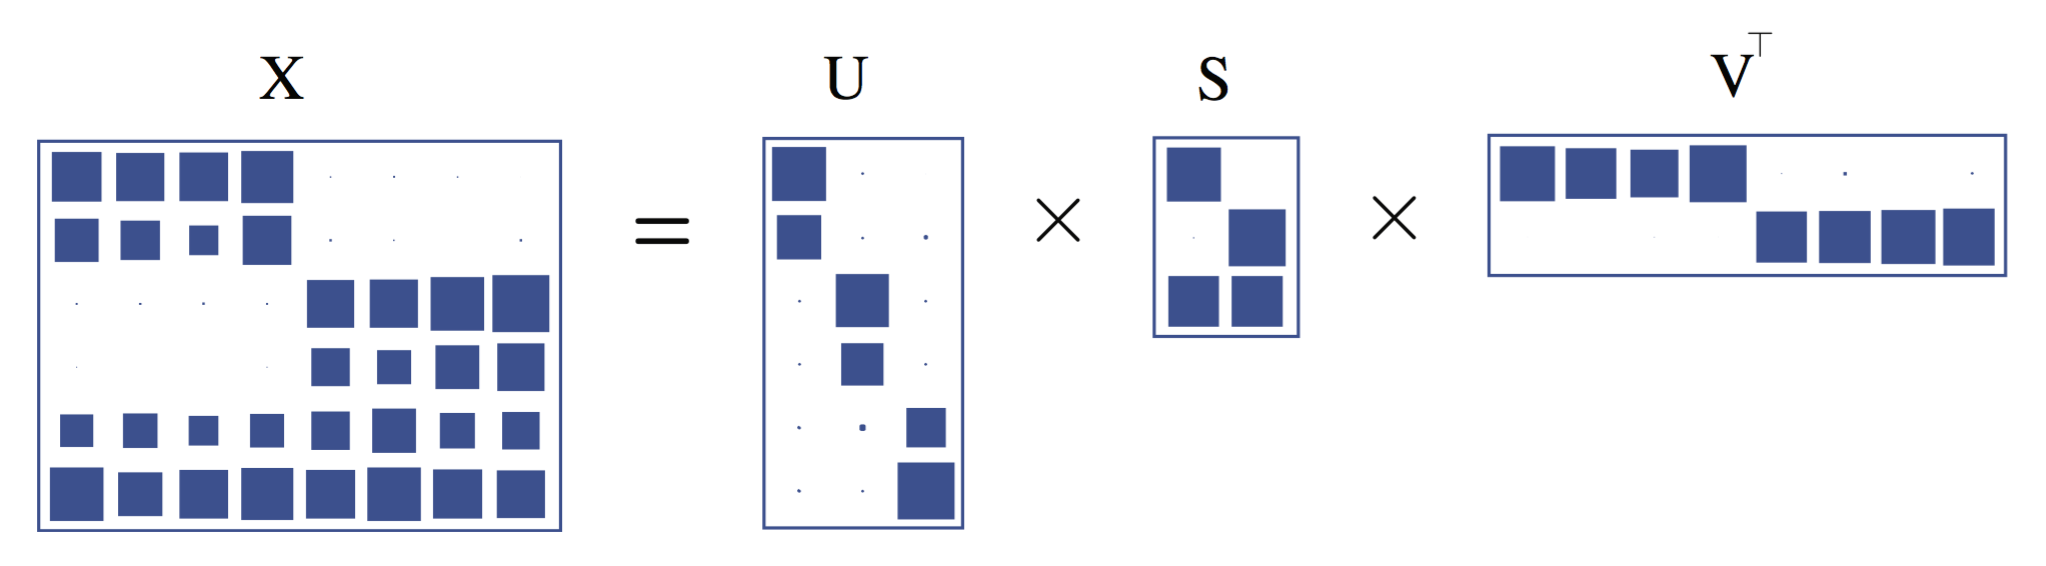
\includegraphics[width=0.7\textwidth]{img/factorizationXUSV.png}
    \label{fig:bvd}
\source{Adaptado de \citeonline{Yoo2010}}
\end{figure}

Na figura~\ref{fig:bvd} considere que uma célula com cor escura representa a existência de uma relação entre linha e coluna, e uma célula com cor clara representa a inexistência de uma relação entre linha e coluna, e que essas relações são estabelecidas adequadamente em cada contexto de aplicação.
Transportando o exemplo da figura para o contexto de uma matriz de ``documentos por palavras'' tem-se um conjunto de seis documentos e quatro palavras, sendo que, por exemplo, o primeiro documento possui uma relação com as duas primeiras palavras, e não possui relação com as terceira e a quarta palavras.
A matriz $U$ pode ser interpretada como uma matriz ``documentos por grupos de documentos'', sendo portanto uma situação em que seis documentos estão agrupados em três grupos ($k = 3$): os dois primeiros documentos no primeiro grupo, os dois próximos no segundo grupo e os dois últimos no terceiro grupo.
A matriz $V^T$ pode ser interpretada como uma matriz de ``grupos de palavras por palavras'', sendo portanto uma situação em que há dois grupos de palavras ($l = 2$) no contexto das quatro palavras existentes.
Finalmente, a matriz $S$ representa uma relação entre ``grupos de documentos'' e ``grupos de palavras''.
A primeira linha da matriz $S$ indica que há uma relação entre o primeiro grupo de linhas e o primeiro grupos de palavras, e que não há uma relação entre o primeiro grupo de linhas e o segundo grupo de palavras.
Seguindo a interpretação intuitiva apresentada por \cite{Long2005}, uma das combinações possíveis, $SV^T$, está ilustrada na figura~\ref{fig:bvd:reconstruction}.
Observe que a matriz $SV^T$ representa ``três grupos de documentos por quatro palavras'', constituindo-se como uma base de representação para grupos de documentos.

\begin{figure}[H]
\centering
    \caption{
        A reconstrução da primeira linha $\mathbf{x}_{1 \cdot}$ de $X$, através da multiplicação da matriz indicadora de grupos de linhas $U$ pela matriz dos protótipos de linhas $(S V^T)$. %que para a primeira linha seleciona apenas o primeiro protótipo,
    }
    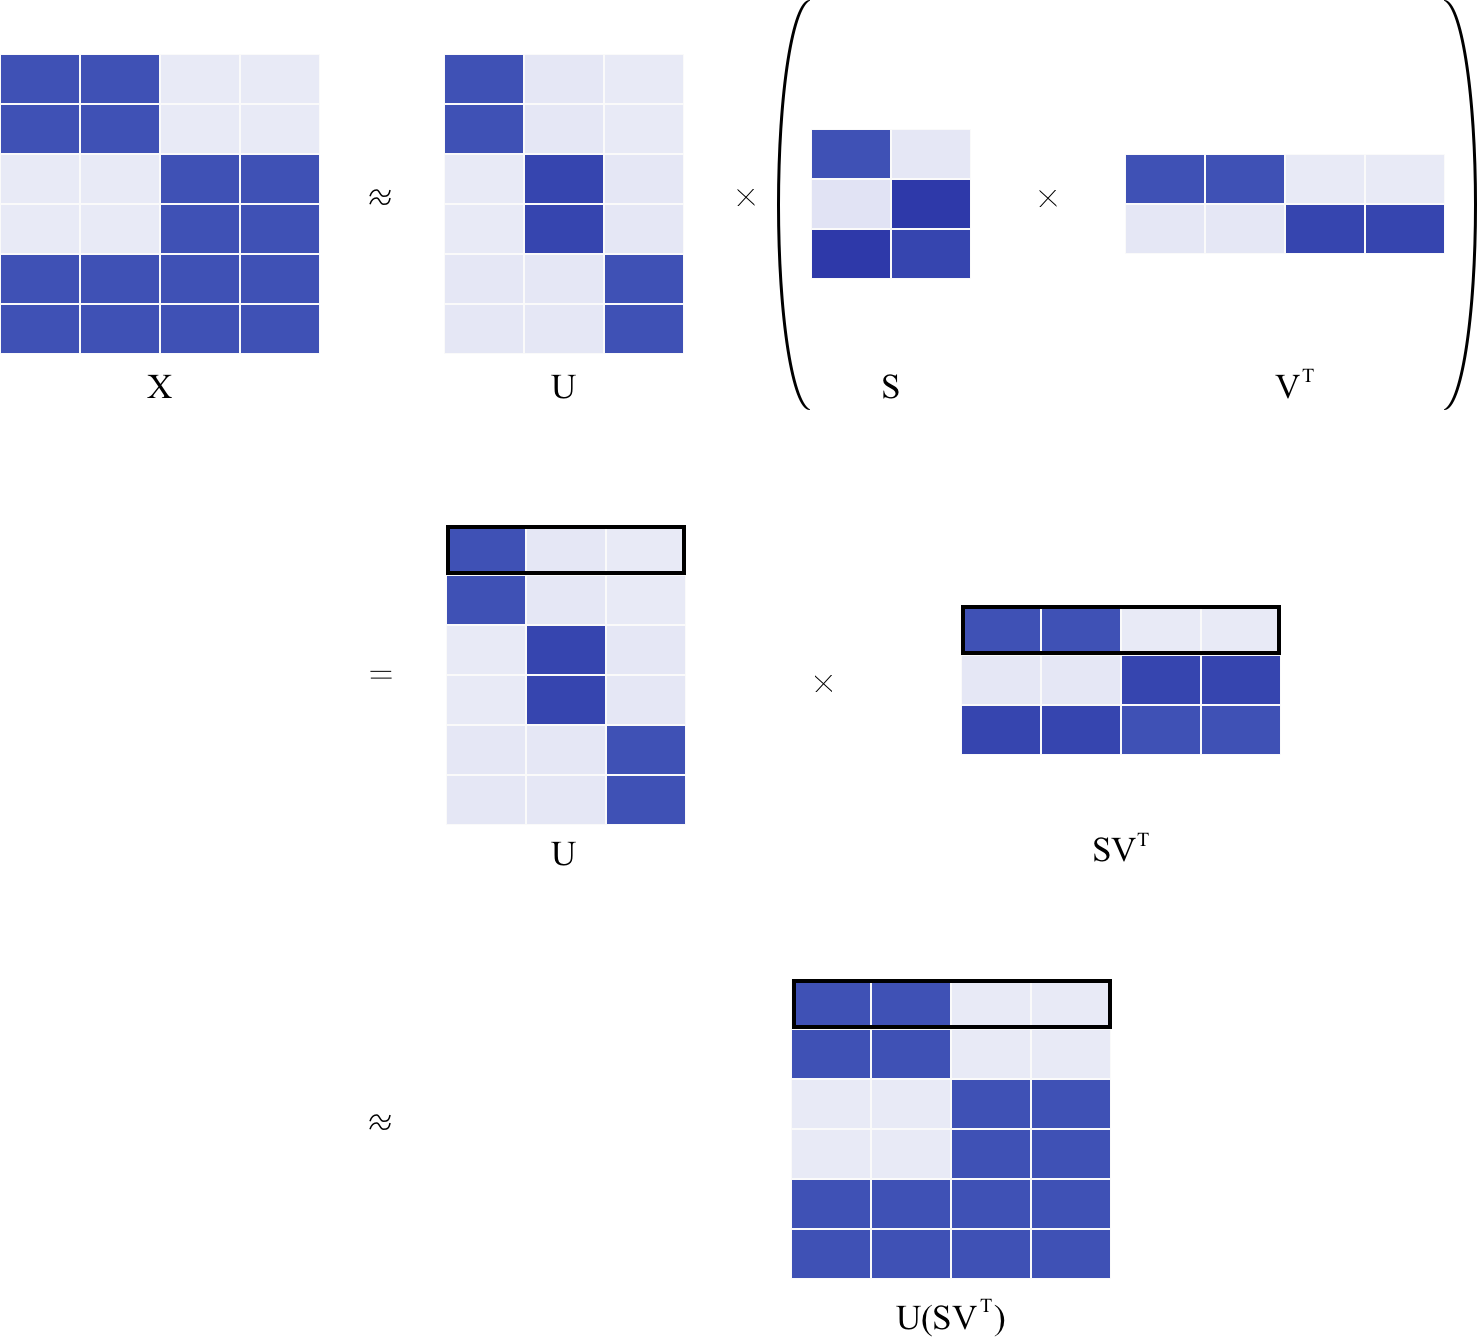
\includegraphics[width=0.7\textwidth]{img/reconstruction.png}
    \label{fig:bvd:reconstruction}
\source{Lucas Fernandes Brunialti, 2016}
\end{figure}

Note ainda que nessa estrutura de matrizes fatoradas é possível identificar protótipos responsáveis por cada parte da reconstrução da matriz original $X$, visto que cada base de representação pode ser vista como um conjunto de vetores protótipos: as linhas de $(SV^T)$ são vetores base (protótipos de grupos de linhas).
O raciocínio apresentado para interpretação da figura~\ref{fig:bvd:reconstruction} pode também ser feito para a interpretação da combinação $US$.
Importante salientar que, assim como ocorre na resolução da tarefa de agrupamento, diferentes grupos de linhas e de colunas podem ser obtidos, representando diferentes soluções para o problema.
E, neste caso ainda, diferentes matrizes $S$ podem ser obtidas para uma mesma organização de grupos de linhas e colunas.
Portanto, qualquer interpretação derivada dessa análise deve ser considerada como apenas uma das formas possíveis de análise dos dados provenientes do contexto de aplicação.\footnote{\textcolor{red}{Medidas de avaliação de agruapmento ou coagrupamento internas podem ser aplicadas às diferentes soluções encontradas de maneira a guiar um processo decisório no contexto de aplicação.}}

Semelhante ao \textit{fuzzy k-means}, é possível observar esta fatoração como uma ótica de compactação.
O BVD compacta a matriz de dados em uma matriz com fatores que correlacionam cada linha com cada grupo de linhas ($U$).
Além disso, esta compactação adiciona a idéia de uma matriz de fatores $V$ para compactar as colunas de $X$, e $S$ que é uma visão compactada de $X$ em $kl$ elementos.
Portanto, a compactação transforma $nm$ elementos em $nk + kl + ml$ elementos, atravéz das matrizes $U$, $S$ e $V$.

O problema de coagrupamento implementado sob a abordagem BVD é formalmente apresentado como \cite{Long2005}:

\begin{problem}[Problema de Decomposição de Valores em Blocos]
\label{def:bvd:problem}
\begin{equation}
    \begin{array}{lclcl}
        \displaystyle \mathcal{F}_1(U, S, V) & = & \displaystyle \min_{U, S, V} & \norm{X - USV^T}^{2}_{F} \\
                                           &   & \text{suj. a}                & U \geq 0,                  \\
                                           &   &                              & S \geq 0,                  \\
                                           &   &                              & V \geq 0
    \end{array}   \nonumber
\end{equation}
\end{problem}

em que $U \in \mathbb{R}^{n \times k}_{+}$, $S \in \mathbb{R}^{k \times l}_{+}$, $V \in \mathbb{R}^{m \times l}$, e $\norm{\cdot}_F$ denota a norma de Frobenius para matrizes.

%% *******************************************************************************************************
%% *******************************************************************************************************
%% *******************************************************************************************************
%% Bom, entendi que essa parte de Lagrange é para provar que o problema vai convergir, então por enquanto comentei visto que nós não vamos fazer provas nos outros algoritmos. Se não for para tirar, voltamos. Como entendi que era para tirar, não li.
%
%Introduzindo a função lagrangeana, associada à $\mathcal{F}_1$:
%\[
%    \displaystyle \mathcal{L}(U, S, V, \Lambda_1, \Lambda_2, \Lambda_3) = \norm{X - USV^T}^{2}_{F} - tr(\Lambda_1 U^T) - tr(\Lambda_2 S^T) - tr(\Lambda_3 V^T) \\
%\]
%
%onde $\Lambda_1 \in \mathbb{R}^{n \times k}$, $\Lambda_2 \in \mathbb{R}^{k \times l}$ e $\Lambda_3 \in \mathbb{R}^{m \times l}$ são os multiplicadores de Lagrange.
%
%Pela teoria de otimização não-linear com restrições, $\Theta = (U^{*}, S^{*}, V^{*}, \Lambda_{1}^*, \Lambda_{2}^*, \Lambda_{3}^*)$ será um mínimo local estacionário de $\mathcal{F}_1$, se e somente se, respeitar as condições de regularidade de \textit{Karush-Kuhn-Tucker} (KKT)~\cite{bazaraa2006}:
%
%\begin{subequations}
%    \begin{alignat}{3}
%        U^* \geq 0, \quad                  && S^* \geq 0, \quad                     && V^* \geq 0                  \label{eq:bvd:kkt1} \\
%        \quad                              && \nabla_{\Theta} \mathcal{L} = 0 \quad &&                             \label{eq:bvd:kkt2} \\
%        \Lambda_{1}^* \odot U^* = 0, \quad && \Lambda_{2}^* \odot S^* = 0, \quad    && \Lambda_{3}^* \odot V^* = 0 \label{eq:bvd:kkt3}
%    \end{alignat}
%\end{subequations}
%
%onde $\odot$ denota o produto de Hadamard.
%
%É possível expandir as equações em~\ref{eq:bvd:kkt2}, calculando as derivadas:
%
%\[
%\begin{array}{lclclclcl}
%    \nabla_U \mathcal{L} & = & U S V^{T} V S^{T}     & - & X V^{T} S^{T} & - & \Lambda_1 & = & 0 \\
%    \nabla_S \mathcal{L} & = & U^{T} U S V^{T} V     & - & U^{T} X V     & - & \Lambda_2 & = & 0 \\
%    \nabla_V \mathcal{L} & = & S^{T} U^{T} U S V^{T} & - & S^{T} U^{T} X & - & \Lambda_3 & = & 0
%\end{array}
%\]
%
%Aplicando o produto Hadamard dos dois lados de cada uma das equações e utilizando das condições em~\ref{eq:bvd:kkt3}:
%\[
%\begin{array}{lclclclclcl}
%    \nabla_U \mathcal{L} & = & U & \odot & U S V^{T} V S^{T}     & - & U & \odot & X V^{T} S^{T} & = & 0 \\
%    \nabla_S \mathcal{L} & = & S & \odot & U^{T} U S V^{T} V     & - & S & \odot & U^{T} X V     & = & 0 \\
%    \nabla_V \mathcal{L} & = & V & \odot & S^{T} U^{T} U S V^{T} & - & V & \odot & S^{T} U^{T} X & = & 0
%\end{array}
%\]
%
%Desta forma, é possível resolver para $U$ de forma algébrica:
%\[
%\begin{array}{lclclcl}
%             & U \odot U S V^{T} V S^{T}                           & = & U \odot X V^{T} S^{T} \\
%    \implies & U \odot \frac{U S V^{T} V S^{T}}{U S V^{T} V S^{T}} & = & U \odot \frac{X V^{T} S^{T}}{U S V^{T} V S^{T}}
%\end{array}
%\]
%
%\[
%    \begin{array}{lclcl}
%        \therefore & U & = & U \odot \frac{X V^{T} S^{T}}{U S V^{T} V S^{T}}
%    \end{array}
%\]
%
%% *******************************************************************************************************
%% *******************************************************************************************************
%% *******************************************************************************************************

A implementação para o processo de minimização do problema~\ref{def:bvd:problem} é descrito no algoritmo~\ref{algo:bvd}, o qual é baseado em atualizações multiplicativas e tem sua convergência demonstrada via teoria de otimização não linear (veja \cite{Long2005}).
Nesse algoritmo considere $t$ o contador de iterações, $U^{(t)}$, $S^{(t)}$ e $V^{(t)}$, as matrizes $U$, $S$ e $V$, na iteração $t$, respectivamente, e $\odot$ é o produto de Hadamard.
% Sara: ué gente, porque t+1 para iteração atual em S e V ????
% Sara: essa ordem de alteração das matrizes está correta??? No artigo não é essa, mas lá não entendi que ele dá a ordem. De onde veio a ordem?

% Lucas: Esse é o mistério, ninguém comenta muito sobre isso, mas na prática só funciona assim, quer dizer, do outro jeito "funciona" tbm, mas a medida de aproximação fica meio louca. A minha idéia é que é assim pq a otimização é alternada, primeiro otimiza pra U fixando S e V, melhora a solução de U, otimiza pra V fixando S e V, melhora a solução de V, otimiza pra S fixando U e V, melhora a solução de S. O mais bizarro é que se foge dessa ordem, a medida de aproximação fica louca.

\begin{algorithm}
\caption{Algoritmo baseado em atualização multiplicativa para solução do BVD}
\label{algo:bvd}
    \begin{algorithmic}[1]
        \Function{BVD}{$X$, $t_{max}$, $k$, $l$}
            \State \textbf{Inicialize:} $U^{(0)} \gets \mathcal{U}(0, 1), V^{(0)} \gets \mathcal{U}(0, 1), S^{(0)} \gets \frac{1}{nm} \sum_{i, j} x_{ij}$ e $t \gets 0$.
            \While{(não convergiu) ou ($t \leq t_{max}$)} %\Comment{We have the answer if r is 0}
                \State
                    \begin{equation}
                    \label{eq:bvd:updateU}
                        U^{(t+1)} \gets U^{(t)} \odot \frac{ X V^{(t)} S^{(t)^T} }{ U^{(t)} S^{(t)} V^{(t)^T} V^{(t)} S^{(t)^T }}             \nonumber
                    \end{equation}
                \State
                    \begin{equation}
                    \label{eq:bvd:updateV}
                        V^{(t+1)} \gets V^{(t)} \odot \frac{ X^T U^{(t+1)} S^{(t)} }{ V^{(t)} S^{(t)^T} U^{(t+1)^T} U^{(t+1)} S^{(t)} }       \nonumber
                    \end{equation}
                \State
                    \begin{equation}
                    \label{eq:bvd:updateS}
                        S^{(t+1)} \gets S^{(t)} \odot \frac{ U^{(t+1)^T} X V^{(t+1)} }{ U^{(t+1)^T} U^{(t+1)} S^{(t)} V^{(t+1)^T} V^{(t+1)} } \nonumber
                    \end{equation}
                \State $t \gets t + 1$
            \EndWhile\label{euclidendwhile}
            \State \textbf{return} $U^{(t)}, S^{(t)}, V^{(t)}$
        \EndFunction
    \end{algorithmic}
\end{algorithm}

A inicialização dos elementos das matrizes $U$, $S$ e $V$ são gerados através de uma distribuição uniforme que ignora zeros ($\mathcal{U}(0, 1) \in~]0, 1]$).
Como condições para assumir a convergência, neste trabalho, considera-se a diferença do erro de aproximação em duas iterações consecutivas menor ou igual a um $\epsilon$:
$$\norm{X - U^{(t)} S^{(t)} V^{(t)^T}}^{2}_{F} - \norm{X - U^{(t+1)} S^{(t+1)} V^{(t+1)^T}}^{2}_{F} \leq \epsilon$$
O algoritmo também pára caso a $t$-ésima iteração seja igual ao número máximo de iterações ($t_{max}$).

Note que como $U$ e $V$ possuem valores no domínio dos reais, então, não é possível obter as partições diretamente, sem um processo de pós-processamento.
Um modo simples de obter o particionamento para as linhas, é o seguinte:
$$\mathcal{K}_p = \mathcal{K}_p + \{ x_{i \cdot} \}~|~p = \argmax_{p'} \mathbf{u}_{i \cdot}~\forall i = \{1, \dots, n\}, \forall p, p' = \{1, \dots, k\}$$

Isso significa que uma linha $i$ pertencerá a um cogrupo $p$ (ou partição) se para todos os $k$ cogrupos, o fator $u_{ip}$ for maior que todos os outros fatores para os outros cogrupos, presentes no vetor $\mathbf{u}_{i \cdot}$.

A complexidade de tempo do algoritmo é possível ser calculada fixando as condições $k \simeq l$, $n \simeq m$, $k << n$, $l << m$ e usando um algoritmo para otimizar a ordem das multiplicações (\citeonline{Cormen2001} discute algoritmos para tal otimização): $\mathcal{O}\Big( t_{max} \big( nl (m + k) + ml (n + k) + mk (n + l) + k^2 (n + l) + l^2 (m + k) \big) \Big)$.


% \begin{theorem}[Corretude]
% \label{def:bvd:correctness}
%     As regras de atualização das equações~\ref{eq:bvd:updateU},~\ref{eq:bvd:updateV} e~\ref{eq:bvd:updateS} são corretas para resolução do problema~\ref{def:bvd:problem}, ou seja, respeitam a condição da equação~\ref{eq:bvd:kkt2}.
% \end{theorem}

% \begin{proof}
%     Esse algoritmo usa o método de iteração de ponto fixo, então, para $U$, se \linebreak
%      $U^{(t)} S^{(t)} V^{(t)^T} V^{(t)} S^{(t)^T} \neq 0$ e $U^{(t + 1)} = U^t \geq 0$, então:
%     \[
%         X V^{(t)^T} S^{(t)^T} = U^{(t)} S^{(t)} V^{(t)^T} V^{(t)} S^{(t)^T} \Rightarrow \nabla_U \mathcal{L} = 0
%     \]
%     verificando a condição da equação~\ref{eq:bvd:kkt2}. O mesmo processo pode ser realizado para $S$ e $V$.
% \end{proof}

% \begin{theorem}[Convergência]
% \label{def:bvd:convergence}
%     O problema~\ref{def:bvd:problem} é decrescente sob as regras de atualização das equações~\ref{eq:bvd:updateU},~\ref{eq:bvd:updateV} e~\ref{eq:bvd:updateS}.
% \end{theorem}

% \begin{proof}
%     % Fixa S e V 1o?
%     Seja uma função auxiliar $G(U)$ para $F(U)$.
% \end{proof}

\section{Fatoração Ortogonal Tripla de Matrizes Não-negativas}
\label{sec:ONMTF}

Baseado no problema~\ref{def:bvd:problem}, \citeonline{Ding06} propõem o problema~\ref{def:onmtf:problem}, e o chama de Fatoração Ortogonal Tripla de Matrizes Não-negativas (\textit{Orthogonal Non-negative Matrix Tri-factorization} - ONMTF).

\begin{problem}[Problema de Fatoração Ortogonal tripla de Matrizes Não-negativas]
\label{def:onmtf:problem}
\begin{equation}
    \begin{array}{lclcl}
        \displaystyle \mathcal{F}_2(U, S, V) & = & \displaystyle \min_{U, S, V} & \norm{X - USV^T}^{2}_{F}      \\
                                             &   & \text{suj. a}                & U \geq 0, S \geq 0, V \geq 0, \\
                                             &   &                              & U^T U = I,                    \\
                                             &   &                              & V^T V = I
    \end{array}   \nonumber
\end{equation}
\end{problem}

em que $U \in \mathbb{R}^{n \times k}_{+}$, $S \in \mathbb{R}^{k \times l}_{+}$, $V \in \mathbb{R}^{m \times l}$ e $\norm{\cdot}_F$ denota a norma de Frobenius.
Na formulação desse problemas, duas restrições de ortonormalidade são acrescentadas, $U^T U = I$ e $V^T V = I$, em que $I$ é a matriz identidade, para as matrizes de grupos de linhas e grupos de colunas, respectivamente.
Tais restrições restringem o problema da fatoração $X \approx USV^T$ para um número menor de possíveis soluções, buscando a unicidade, como mostrado na figura~\ref{fig:bvdvsonmtf}.
No entanto, o algoritmo não garante que as restrições de ortonomalidade são respeitadas, apesar das restrições colocadas encontrarem soluções de particionamento com maior ortogonalidade.

% $U \geq 0, S \geq 0, V \geq 0$ sendo todos os elementos de $U$, $S$ e $V$, maior que $0$, respectivamente, $U^T U = I$ e $V^T V = I$ as restrições de ortonomalidade para as matrizes indicadoras de grupos de linhas e colunas, respectivamente, e $\norm{\cdot}_F$ denota a norma de Frobenius para matrizes.

\begin{figure} [htpb]
\centering
    \caption{Base de protótipos obtidas com FMN sem restrições (a) e com restrições de ortogonalidade nas matrizes}
    \begin{subfigure}[b]{0.3\textwidth}
        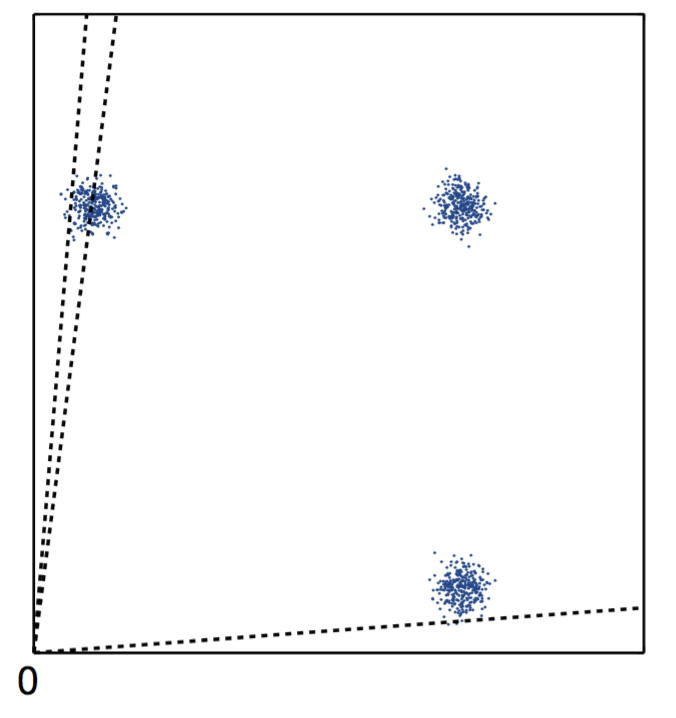
\includegraphics[width=\textwidth]{img/bvdVsOnmtf1.png}
        \caption{}
        \label{fig:bvdvsonmtf:1}
    \end{subfigure}
    ~ %add desired spacing between images, e. g. ~, \quad, \qquad, \hfill etc.
      %(or a blank line to force the subfigure onto a new line)
    \begin{subfigure}[b]{0.3\textwidth}
        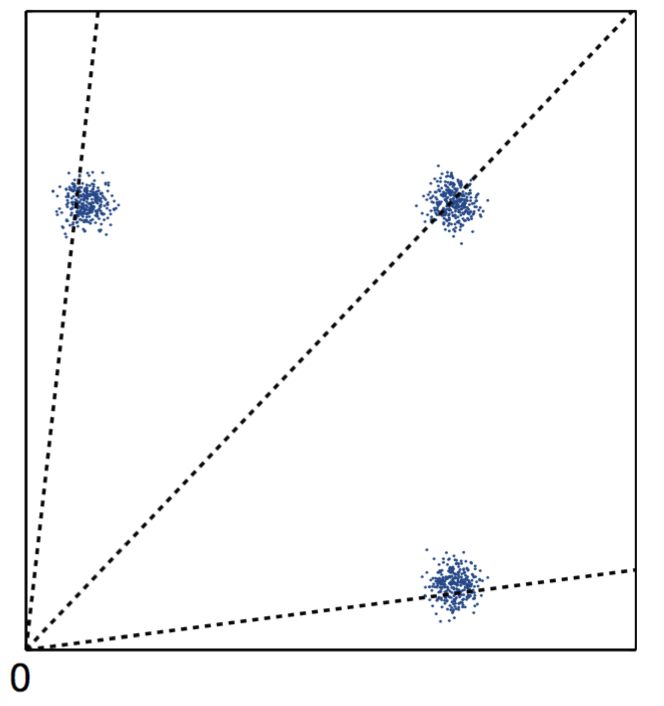
\includegraphics[width=\textwidth]{img/bvdVsOnmtf2.png}
        \caption{}
        \label{fig:bvdvsonmtf:2}
    \end{subfigure}

 %       Um exemplo sintético que compara o algoritmo para BVD contra o algoritmo para ONMTF, com pontos sendo dados, as linhas pontilhadas sendo os protótipos de linhas ($S V^T$), e os três conjuntos de pontos sendo os grupos. (a) O algoritmo para BVD encontra uma solução com dois protótipos em um mesmo grupo, deixando um dos grupos sem nenhum protótipo para representá-lo. Apesar de ser uma solução correta, ou seja, encontra um mínimo local, não é a desejada. (b) O algoritmo para ONMTF é capaz de encontrar a solução em que cada protótipo aproxima cada grupo de dados, através das restrições referentes à ortogonalidade, este é capaz de restringir as possíveis soluções para a fatoração $X \approx U S V^T$.

    \label{fig:bvdvsonmtf}
    \source{\citeonline{Yoo2010}}
\end{figure}

A figura~\ref{fig:bvdvsonmtf} representa um problema com três grupos (três nuvens de pontos).
As linhas pontilhadas representam os protótipos obtidos por FMN (a) sem restrição de ortogonalidade nas matrizes, como o BVD (a), e (b) com restrição de ortogonalidade nas matrizes, como o ONMTF.
Note que a base obtida com FMN ortogonal tende a encontrar protótipos mais centralizados nos grupos.
Já a base obtida com FMN sem restrições tende a encontrar uma região convexa que contém os pontos dos grupos (incluindo regiões que abrangem pontos de grupos originalmente projetados como sendo diferentes).
A solução obtida em (a), embora correta, não é desejável.

Em termos de compactação, igualmente ao BVD, o algoritmo para solução do ONMTF transforma os $nm$ elementos da matriz $X$ em $nk + kl + ml$ elementos, atravéz da fatoração em $U$, $S$ e $V$.

\citeonline{Ding06} propõem uma solução para implementação do processo de minimização para o problema~\ref{def:onmtf:problem} semelhante ao que foi apresentado na seção~\ref{sec:bvd}, também baseado em atualizações multiplicativas e com convergência demonstrada com base na teoria de otimização não linear.
O algoritmo para tal processo de minimização é apresentado no algoritmo~\ref{algo:onmtf}, no qual $t$ o contador de iterações, $U^{(t)}$, $S^{(t)}$ e $V^{(t)}$, as matrizes $U$, $S$ e $V$, na iteração $t$, respectivamente, $\odot$ é o produto de Hadamard e $\mathcal{U}(0, 1) \in~]0, 1]$ uma função que gera valores de uma distribuição uniforme que ignora zeros.
Também, a mesma condição de convergência aplicada no algoritmo~\ref{algo:bvd} pode ser aplicada nesse caso.

%fazendo a derivação através da função lagrangeana e a introdução dos multiplicadores de lagrange, utilizando as condições de otimização não-linear de KKT, derivando as regras para atualização multiplicativa para $U$, $S$ e $V$, apresentadas no algoritmo~\ref{algo:onmtf}.

\begin{algorithm}
\caption{Algoritmo baseado em atualização multiplicativa para solução do ONMTF}
\label{algo:onmtf}
    \begin{algorithmic}[1]
        \Function{ONM3F}{$X$, $t_{max}$, $k$, $l$}
            \State \textbf{Inicialize:} $U^{(0)} \gets \mathcal{U}(0, 1), V^{(0)} \gets \mathcal{U}(0, 1), S^{(0)} \gets \mathcal{U}(0, 1)$ e $t \gets 0$.
            \While{(não convergiu) ou ($t \leq t_{max}$)} %\Comment{We have the answer if r is 0}
                \State
                    \begin{equation}
                    \label{eq:onmtf:updateU}
                        U^{(t+1)} \gets U^{(t)} \odot \sqrt{ \frac{ X V^{(t)} S^{(t)^T} }{ U^{(t)} U^{(t)^T} X V^{(t)} S^{(t)^T} } }
                    \end{equation}
                \State
                    \begin{equation}
                    \label{eq:onmtf:updateV}
                        V^{(t+1)} \gets V^{(t)} \odot \sqrt{ \frac{ X^T U^{(t+1)} S }{ V^{(t)} V^{(t)^T} X^T U^{(t+1)} S^{(t)} } }
                    \end{equation}
                \State
                    \begin{equation}
                    \label{eq:onmtf:updateS}
                        S^{(t+1)} \gets S^{(t)} \odot \sqrt{ \frac{ U^{(t+1)^T} X V^{(t+1)} }{ U^{(t+1)^T} U^{(t+1)} S^{(t)} V^{(t+1)^T} V^{(t+1)} } }
                    \end{equation}
                \State $t \gets t + 1$
            \EndWhile\label{euclidendwhile}
            \State \textbf{return} $U^{(t)}, S^{(t)}, V^{(t)}$
        \EndFunction
    \end{algorithmic}
\end{algorithm}

Note que é possível obter o particionamento de linhas e colunas da mesma forma que foi descrita com o BVD.
Calculando a complexidade de tempo, fixando as mesmas condições $k \simeq l$, $n \simeq m$, $k << n$, $l << m$ e usando um algoritmo para otimizar a ordem das multiplicações, é possível encontrar a mesma complexidade antes calculada para o algoritmo~\ref{algo:bvd}.

% Sara: \textcolor{red}{Note que no algoritmo ONMTF, a matriz de dados de entrada é considerada .... não deveríamos falar alguma coisa aqui sobre as principais diferenças das regras de atualização das matrizes????}

%     \label{eq:onmtf:updateU}
%         U^{(t+1)} \gets U^{(t)} \odot \frac{ X V^{(t)} S^{(t)^T} }{ U^{(t)} U^{(t)^T} X V^{(t)} S^{(t)^T} }      \nonumber
%     \end{equation}
% \State
%     \begin{equation}
%     \label{eq:onmtf:updateV}
%         V^{(t+1)} \gets V^{(t)} \odot \frac{ X^T U^{(t+1)} S }{ \textcolor{blue}{V^{(t)} V^{(t)^T}} X^T U^{(t+1)} S^{(t)} }      \nonumber
%     \end{equation}
% \State
%     \begin{equation}
%     \label{eq:onmtf:updateS}
%         S^{(t+1)} \gets S^{(t)} \odot \frac{ U^{(t+1)^T} X \textcolor{blue}{V^{(t+1)}} }{ U^{(t+1)^T} U^{(t+1)} S^{(t)} \textcolor{blue}{V^{(t+1)^T} V^{(t+1)}} }    \nonumber
%     \end{equation}

%%% *****************************************************************************************************
%%% *****************************************************************************************************
%%% *****************************************************************************************************

% Novamente, entendendo que aqui temos uma reprodução direta do artigo e que isso não precisa ser reproduzido, coloquei em comentário. Se precisar voltar ok, mas eu não li essa parte ainda.

No artigo de \citeonline{Yoo2010}, é proposta uma abordagem mais simples para a derivação das regras de atualização multiplicativas, considere uma função de otimização qualquer $\mathcal{J}$ e seu respectivo gradiente $\nabla \mathcal{J}$:

\[
   \begin{array}{lclcl}
       \nabla \mathcal{J} & = & [\nabla \mathcal{J}]^+ - [\nabla \mathcal{J}]^-
   \end{array}
\]

onde $[\nabla \mathcal{J}]^+$ é a parte positiva do gradiente, $[\nabla \mathcal{J}]^-$ a parte negativa do gradiente.
Se $[\nabla \mathcal{J}]^+ \geq 0$ e $[\nabla \mathcal{J}]^- \geq 0$, então, é possível definir uma regra de atualização multiplicativa, para otimizar os parâmetros $\Theta$ da função $\mathcal{J}$:

\begin{equation}
\label{eq:onmtf:updateTheta}
   \Theta \gets \Theta \odot \left ( \frac{ [\nabla \mathcal{J}]^- }{ [\nabla \mathcal{J}]^+ } \right )^{\cdot \eta}
\end{equation}

onde $\odot$ representa o produto Hadamard, $(\cdot)^{\cdot \eta}$ representa a potência para cada elemento, e $\eta$ uma taxa de aprendizado ($0 < \eta \leq 1$).
Então, se $\Theta$ for inicializado com elementos positivos, é possível verificar que a regra de atualização multiplicativa da equação~\ref{eq:onmtf:updateTheta} mantém a não-negatividade de $\Theta$.

Também, é utilizada uma abordagem diferente para a derivação de regras de atualização multiplicativas, visando um algoritmo para a solução do problema~\ref{def:onmtf:problem}.
Neste caso, o gradiente é calculado com base em uma superfície com restrições que preserva a ortogonalidade.
Essa superfície com restrições é chamada de Variedade de Stiefel (\textit{Stiefel Manifold}).

%Também, é utilizada uma abordagem diferente para a derivação de regras de atualização multiplicativas, visando um algoritmo para a solução do problema~\ref{def:onmtf:problem}.
%Neste caso, o gradiente é calculado com base em uma superfície com restrições que preserva a ortogonalidade.
%Essa superfície com restrições é chamada de Variedade de Stiefel (\textit{Stiefel Manifold}), neste caso é usada a Variedade de Stiefel no espaço euclidiano, denotada por $\mathcal{H}_{a,b}$, sendo essa variedade o conjunto de $a \times b$ matrizes ortonormais no espaço $\mathbb{R}^a$, formalmente:

%\[
%    \begin{array}{lclcl}
%        \mathcal{H}_{a, b} & = & \{ Y \in \mathbb{R}^{a \times b}: Y^T Y = I \}
%    \end{array}
%\]

%Note que quando $b = 1$, a superfície se torna uma esfera.
%Para otimização, considerando que essa esfera sejam as restrições do problema, o ideal é propor métodos que permanecam na esfera, então, todos os vetores tangentes à essa esfera, podem ser direções possíveis para um algoritmo de otimização iterativo, como mostra a Figura~\ref{fig:stiefel}.

%\begin{figure}[H]
%\centering
%    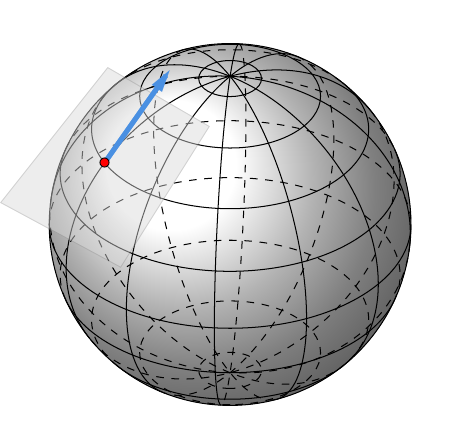
\includegraphics[width=0.3\textwidth]{img/stiefel.png}
%    \caption{
%        Uma Variedade Stiefel no espaço Euclidiano, que quando $b = 1$ essa superfície será uma esfera, e um dos possíveis vetores que está contido no conjunto dessa variedade (tangente à esfera).
%    }
%    \label{fig:stiefel}
%\end{figure}

%\citeonline{Edelman1999} definem o gradiente em um ponto $Y$, com a restrição $Y^T Y = I$, de uma função $\mathcal{J}$ definida em uma Variedade Stiefel no espaço euclidiano como:

%\begin{equation}
%\label{eq:stiefeldiff}
%    \begin{array}{lclcl}
%        {\tilde \nabla}_Y \mathcal{J} & = & \nabla_Y \mathcal{J} - Y (\nabla_Y \mathcal{J})^T Y
%    \end{array}
%\end{equation}

%onde $\nabla_Y \mathcal{J}$ é o gradiente da função $\mathcal{J}$ para todos os elementos da matriz $Y$.

%Dada a equação~\ref{eq:stiefeldiff}, \citeonline{Yoo2010} propõem os seguintes cálculos dos gradientes em Variedades Stiefel para $\mathcal{F}_2$, com $U$ no conjunto $\{ U^T U = I \}$, e com $V$ no conjunto $\{ V^T V = I \}$:

%\[
%    \begin{array}{lclclclcl}
%        {\tilde \nabla_U} \mathcal{F}_2 & = & \nabla_U \mathcal{F}_2 - U (\nabla_U \mathcal{F}_2)^T U & = & U S V^T X^T U - X V S^T \\
%        {\tilde \nabla_V} \mathcal{F}_2 & = & \nabla_V \mathcal{F}_2 - V (\nabla_V \mathcal{F}_2)^T V & = & V S^T U^T X V - X^T U S
%    \end{array}
%\]

%Restando apenas o cálculo do gradiente para $S$, que como não há restrições, será igual à atualização do algoritmo para solução do BVD:

%\[
%    \begin{array}{lclcl}
%        {\tilde \nabla_S} \mathcal{F}_2 & = & \nabla_S \mathcal{F}_2 & = & U^T U S V^T V - U^T X V
%    \end{array}
%\]

Assim,~\citeonline{Yoo2010} faz o uso da estratégia da equação~\ref{eq:onmtf:updateTheta} e da teoria de derivação na superfície com restrições (Variedade Stiefel), para propor uma solução para o problema~\ref{def:onmtf:problem} (ONMTF) alternativa às atualizações das equações~\ref{eq:onmtf:updateU},~\ref{eq:onmtf:updateV} e~\ref{eq:onmtf:updateS}, através da atualização multiplicativa.
Essas atualizações são apresentadas no algoritmo~\ref{algo:onmtf2}, considere $t$ o contador de iterações, $U^{(t)}$, $S^{(t)}$ e $V^{(t)}$, as matrizes $U$, $S$ e $V$, na iteração $t$, respectivamente, $\odot$ o produto de Hadamard, $\mathcal{U}(0, 1) \in~]0, 1]$ uma função que gera valores de uma distribuição uniforme que ignora zeros, $\diag( \cdot )$ uma função que extrai a diagonal principal de uma matriz e a transforma em um vetor, e $\mathbf{1}$ um vetor de uns com dimensão que torne a multiplicação possível.

Considerando a preservação da ortonormalidade, o algoritmo apresentado é capaz de preservar melhor a ortonormalidade.
Para tal afirmação,~\citeonline{Yoo2010} realizou um experimento que consistiu em medir as restrições de ortonormalidade em $U$ e $V$, através das restrições $\norm{U^T U - I}$ e $\norm{V^T V - I}$, respectivamente, durante cada iteração do algoritmo proposto, comparando-o com o algoritmo proposto por~\citeonline{Ding06}.

\begin{algorithm}
\caption{Algoritmo baseado em atualização multiplicativa e na teoria de de derivação na superfície com restrições (Variedade Stiefel) para solução do ONMTF}
\label{algo:onmtf2}
    \begin{algorithmic}[1]
        \Function{ONMTF}{$X$, $t_{max}$, $k$, $l$}
            \State \textbf{Inicialize:} $U^{(0)} \gets \mathcal{U}(0, 1), V^{(0)} \gets \mathcal{U}(0, 1), S^{(0)} \gets \mathcal{U}(0, 1)$ e $t \gets 0$.
            \While{(não convergiu) ou ($t \leq t_{max}$)} %\Comment{We have the answer if r is 0}
                \State
                    \begin{equation}
                        U^{(t+1)} \gets U^{(t)} \odot \frac{ X V^{(t)} S^{(t)^T} }{ U^{(t)} S^{(t)} V^{(t)^T} X^T U^{(t)} } \nonumber
                    \end{equation}
                \State
                    \begin{equation}
                        V^{(t+1)} \gets U^{(t)} \odot \frac{ X^T U^{(t+1)} S^{(t)} }{ V^{(t)} S^{(t)^T} U^{(t+1)^T} X V^{(t)} } \nonumber
                    \end{equation}
                \State
                    \begin{equation}
                        S^{(t+1)} \gets S^{(t)} \odot \frac{ U^{(t+1)^T} X V^{(t+1)} }{ U^{(t+1)^T} U^{(t+1)} S^{(t)} V^{(t+1)^T} V^{(t+1)} } \nonumber
                    \end{equation}
                \State $t \gets t + 1$
            \EndWhile\label{euclidendwhile}
            \State
                $$U^{(t)} \gets U^{(t)} \diag(S^{(t)} \diag(\mathbf{1}^T V^{(t)}) \mathbf{1})$$
            \State
                $$V^{(t)} \gets V^{(t)} \diag(\mathbf{1}^T \diag(\mathbf{1}^T U^{(t)}) S^{(t)})$$
            \State \textbf{return} $U^{(t)}, S^{(t)}, V^{(t)}$
        \EndFunction
    \end{algorithmic}
\end{algorithm}

Ainda,~\citeonline{Yoo2010} propõem uma normalização baseada numa interpretação probabilística da fatoração de $X$ em $USV^T$, para então realizar o particionamento de linhas e colunas, como apresentado no algoritmo~\ref{algo:onmtf2}.
Note que o particionamento de linhas e colunas é realizado como nos outros algoritmos já apresentados e a mesma condição de convergência aplicada no algoritmo~\ref{algo:bvd} e~\ref{algo:onmtf} pode ser aplicada nesse caso.

Calculando a complexidade de tempo, seguindo as mesmas restrições apresentadas anteriormente para os outros algoritmos, é possível verificar que o algoritmo~\ref{algo:onmtf2},proposto por~\citeonline{Yoo2010} para solução do problema~\ref{def:onmtf:problem} (ONMTF), é equivalente à complexidade apresentada para o algoritmo~\ref{algo:bvd} e~\ref{algo:onmtf}.

\section{Fatoração Tripla Rápida de Matrizes Não-negativas}
\label{sec:FNMTF}

O problema de Fatoração Tripla Rápida de Matrizes Não-negativas (\textit{Fast Non-negative Matrix Tri Factorization} - FNMTF), formalizado no problema~\ref{def:fnmtf:problem}, foi proposto por \citeonline{Wang2011} com os seguintes argumentos contra o uso prático dos problemas até então propostos para encontrar cogrupos: eles exigem soluções algorítmicas iterativas, com intensas multiplicações de matrizes em cada passo do algoritmo; eles propõem encontrar coagrupamentos flexíveis (com restrições relaxadas), o que implica em encontrar inúmeras soluções para a tarefa de coagrupamento.

\begin{problem}[Fatoração tripla rápida de Matrizes Não-negativas]
\label{def:fnmtf:problem}
\begin{equation}
    \begin{array}{lclcl}
        \displaystyle \mathcal{F}_3(U, S, V) & = & \displaystyle \min_{U, S, V} & \norm{X - USV^T}^{2}_{F} \\
                                             &   &                              & U \in \Psi^{n \times k}, \\
                                             &   &                              & V \in \Psi^{m \times l}
    \end{array} \nonumber
\end{equation}
\end{problem}

em que $S \in \mathbb{R}^{k \times l}_{+}$, $\Psi = \{0, 1\}$, $\sum_{p=1}^{k} \mathbf{u}_{p \cdot} = 1$ e $\sum_{q=1}^{l} \mathbf{v}_{q \cdot} = 1$.

\citeonline{Wang2011} denominam $U$ como uma matriz indicadora dos grupos de linhas, $V$ como uma matriz indicadora dos grupos de colunas, e $S$ como uma matriz que contém os fatores que relacionam um grupo de linhas aos grupos de colunas, e um grupo de colunas aos grupos de linhas.
Note que nesse caso não é necessário uma etapa de pós-processamento para particionamento como nos outros algoritmos apresentados.

Ainda, as restrições $\sum_{p=1}^{k} \mathbf{u}_{p \cdot} = 1$ e $\sum_{q=1}^{l} \mathbf{v}_{q \cdot} = 1$ indicam que uma linha e uma coluna, respectivamente, têm que pertencer à algum grupo.
Então, apesar dessas restrições serem semelhantes à ortonormalidade, elas não são, pois não resolvem o caso em que há uma possibilidade de haver grupos vazios, ou seja, sem nenhum elemento pertencente a este grupo, enquanto a restrição de ortonormalidade, garante que não haverá grupos vazios, seja este grupo de linhas ou de colunas.

Como $U$ e $V$ neste caso têm as restrições descritas, e são capazes de fornecer o particionamento de linhas e colunas, respectivamente, de forma direta, a capacidade de compactação nesse caso é semelhante ao algoritmo \textit{k-means}, brevemente descrito no Capítulo~\ref{ch:conceitos}.
Porém, como a fatoração compacta as colunas e as relações entre grupos de linhas e colunas (matriz $S$), a matriz $X$ é compactada em $n + kl + m$ elementos.

Como não há restrições em $S$, com exceção da positividade que é garantida pela positividade de $X$, é possível encontrar uma regra de atualização para $S$, e portanto, minimização de $\mathcal{F}_3$:
\[
    \begin{array}{lclcl}
        \nabla_S \mathcal{F}_3 &     =    & U^T X V - U^T U S V^T V                     & = & 0                             \\
                               & \implies & U^T U S V^T V                               & = & U^T X V                       \\
                               & \implies & (U^T U)^{-1} U^T U S V^T V (V^T V)^{-1} & = & (U^T U)^{-1} U^T X V (V^T V)^{-1}
    \end{array}   \nonumber
\]

\begin{equation}
\label{eq:fnmtf:updateS}
    \begin{array}{lclcl}
        \therefore & S & = & (U^T U)^{-1} U^T X V (V^T V)^{-1}    \nonumber
    \end{array}
\end{equation}

Assim, o problema de minimização se transforma nos subproblemas de atualização de $U$ e $V$.
Uma estratégia semelhante aquela aplicada no clássico algoritmo \textit{k-means} pode ser aplicada.
Primeiramente, fixa-se $S$ e $V$ e resolve-se o problema~\ref{def:fnmtf:problem} para $U$ de forma iterativa, verificando quais dos protótipos de linhas (linhas de $\widetilde{V}$) mais se aproxima das linhas de $X$.
Em seguida, fixa-se $S$ e $U$ para alcançar uma solução iterativa para $V$, através dos protótipos de colunas (colunas de $\widetilde{U}$), assim como mostrado no algoritmo~\ref{algo:fnmtf}.

Note que é possível interpretar a regra de atualização para $S$: $(U^T U)$ é uma matriz que na diagonal contém a contagem do número de linhas em cada grupo de linhas e zeros nas demais posições, $(U^T U)^{-1}$ é o cálculo da média parcial para cada grupo de linhas, e $U^T X$ seleciona e soma as linhas de $X$ para cada grupo de linhas.
A mesma interpretação pode ser feita para $(V^T V)$, $(V^T V)^{-1}$ e $XV$.
O seguinte exemplo mostra uma matriz de dados com $6$ linhas e $3$ colunas, particionada por $3$ grupos de linhas e $2$ grupos de colunas, ilustrando a interpretação da atualização de $S$:
\[
    X = \begin{bmatrix}
            \horzbar & \mathbf{x}_{1 \cdot} & \horzbar \\
            \horzbar & \mathbf{x}_{2 \cdot} & \horzbar \\
            \horzbar & \mathbf{x}_{3 \cdot} & \horzbar \\
            \horzbar & \mathbf{x}_{4 \cdot} & \horzbar \\
            \horzbar & \mathbf{x}_{5 \cdot} & \horzbar \\
            \horzbar & \mathbf{x}_{6 \cdot} & \horzbar
        \end{bmatrix}
      = \begin{bmatrix}
            \vertbar             & \vertbar             & \vertbar             \\
            \mathbf{x}_{\cdot 1} & \mathbf{x}_{\cdot 2} & \mathbf{x}_{\cdot 3} \\
            \vertbar             & \vertbar             & \vertbar
        \end{bmatrix}
\]
\[
    U = \begin{bmatrix}
           1 & 0 & 0 \\
           1 & 0 & 0 \\
           0 & 1 & 0 \\
           0 & 0 & 1 \\
           0 & 1 & 0 \\
           1 & 0 & 0
         \end{bmatrix},
    U^T U = \begin{bmatrix}
                3 & 0 & 0 \\
                0 & 2 & 0 \\
                0 & 0 & 1
            \end{bmatrix},
    V = \begin{bmatrix}
            0 & 1 \\
            0 & 1 \\
            1 & 0
        \end{bmatrix},
    V^T V = \begin{bmatrix}
                1 & 0 \\
                0 & 2
            \end{bmatrix}
\]
A matriz $U$ do exemplo, apresenta um particionamento das $6$ linhas em $3$ grupos, sendo que $3$ linhas pertencem ao primeiro grupo, $2$ linhas ao segundo grupo, e $1$ linha ao terceiro grupo, como mostra a diagonal principal da matriz $U^T U$, a mesma interpretação pode ser feita para $V$ e $V^T V$.
\[
    \begin{array}{ll}
        (U^T X) V & = \Bigg(\begin{bmatrix}
                                1 & 1 & 0 & 0 & 0 & 1 \\
                                0 & 0 & 1 & 0 & 1 & 0 \\
                                0 & 0 & 0 & 1 & 0 & 0
                            \end{bmatrix}
                            \begin{bmatrix}
                                \horzbar & \mathbf{x}_{1 \cdot} & \horzbar \\
                                \horzbar & \mathbf{x}_{2 \cdot} & \horzbar \\
                                \horzbar & \mathbf{x}_{3 \cdot} & \horzbar \\
                                \horzbar & \mathbf{x}_{4 \cdot} & \horzbar \\
                                \horzbar & \mathbf{x}_{5 \cdot} & \horzbar \\
                                \horzbar & \mathbf{x}_{6 \cdot} & \horzbar
                            \end{bmatrix}\Bigg)
                            \begin{bmatrix}
                                0 & 1 \\
                                0 & 1 \\
                                1 & 0
                            \end{bmatrix}
                    = \begin{bmatrix}
                          \mathbf{x}_{1 \cdot} + \mathbf{x}_{2 \cdot} + \mathbf{x}_{6 \cdot} \\
                          \mathbf{x}_{3 \cdot} + \mathbf{x}_{5 \cdot}                        \\
                          \mathbf{x}_{4 \cdot}
                      \end{bmatrix}
                      \begin{bmatrix}
                          0 & 1 \\
                          0 & 1 \\
                          1 & 0
                      \end{bmatrix} \\
                  & = \begin{bmatrix}
                          x_{13} + x_{23} + x_{63} & x_{11} + x_{12} + x_{21} + x_{22} + x_{61} + x_{62} \\
                          x_{33} + x_{53}          & x_{31} + x_{32} + x_{51} + x_{52}                   \\
                          x_{43}                   & x_{41} + x_{42}
                      \end{bmatrix}
    \end{array}
\]
A multiplicação em $X$ por $U^T$ pela esquerda, representa a soma da seleção de todas as linhas de $X$ pertencentes à um mesmo grupo de linhas.
O mesmo ocorre quando multiplica-se $V$ pela direita de $X$, porém, representando a soma da seleção das colunas de $X$ pertencentes à um mesmo grupo de colunas.
Sendo assim, a operação $U^T X V$ representa a soma de todos os elementos de $X$ pertencentes à um mesmo grupo de linhas e colunas, ou seja, por exemplo o elemento da linha $1$ e coluna $1$ de $U^T X V$, que foi calculado no exemplo, é simplesmente a soma de todos os elementos de $X$ que pertencem ao primeiro grupo de linhas e ao primeiro grupo de colunas.\tabularnewline
\[
    (U^T U)^{-1} = \begin{bmatrix}
                       \frac{1}{3} & 0           & 0 \\
                       0           & \frac{1}{2} & 0 \\
                       0           & 0           & 1
                   \end{bmatrix},
    (V^T V)^{-1} = \begin{bmatrix}
                       1 & 0           \\
                       0 & \frac{1}{2}
                   \end{bmatrix}
\]
\[
    S = (U^T U)^{-1} U^T X V (V^T V)^{-1} = \begin{bmatrix}
                                                \frac{x_{13} + x_{23} + x_{63}}{3} & \frac{x_{11} + x_{12} + x_{21} + x_{22} + x_{61} + x_{62}}{3 \times 2} \\
                                                \frac{x_{33} + x_{53}}{2}          & \frac{x_{31} + x_{32} + x_{51} + x_{52}}{2 \times 2}                   \\
                                                x_{43}                             & \frac{x_{41} + x_{42}}{2}
                                            \end{bmatrix}
\]
Com o exemplo mostrado, é possível visualizar a atualização de $S$ de forma mais intuitiva.
Por exemplo, para calcular um elemento $s_{pq}$ de $S$, será simplesmente o cálculo da média de todos elementos em $X$ que pertencem ao grupo de linhas $p$ e ao grupo de colunas $q$.
Dessa forma, também é possível propor uma solução iterativa para $S$.

O algoritmo~\ref{algo:fnmtf} ilustra o processo de minimização para o problema~\ref{def:fnmtf:problem}.
Nesse algoritmo considere os índices $i = \{1, \dots, n\}$, $j = \{1, \dots, m\}$, $p = p' = \{1, \dots, k\}$, e $q = q' = \{1, \dots, l\}$, o contador de iterações $t$, $U^{(t)}$, $S^{(t)}$ e $V^{(t)}$ como sendo as matrizes $U$, $S$ e $V$ na iteração $t$, respectivamente, $\mathcal{U}(0, 1) \in~]0, 1]$ uma função que gera valores de uma distribuição uniforme que ignora zeros, e $\norm{ \cdot }^2$ é a norma frobenius para vetores.
Também, as mesmas condições de convergência usada nos algoritmos anteriores pode ser aplicada nesse caso.

\begin{algorithm}
\caption{Algoritmo FNMTF}
\label{algo:fnmtf}
    \begin{algorithmic}[1]
        \Function{FNMTF}{$X$, $t_{max}$, $k$, $l$}
            \State \textbf{Inicialize:} $U^{(0)}, V^{(0)} \gets {0,1}~|~\sum_{p=1}^{k} \mathbf{u}_{p \cdot} = 1, \sum_{q=1}^{l} \mathbf{v}_{q \cdot} = 1$, $S^{(0)} \gets \mathcal{U}(0, 1)$ e $t \gets 0$.
            \While{(não convergiu) ou ($t \leq t_{max}$)}
                \State
                    \begin{equation}
                    \label{eq:fnmtf:updateS}
                        S^{(t+1)} \gets (U^{(t)^T} U^{(t)})^{-1} U^{(t)^T} X V^{(t)} (V^{(t)^T} V^{(t)})^{-1}   \nonumber
                    \end{equation}
                \State
                    \[
                        \widetilde{V} \gets S^{(t+1)} V^{(t)^T}
                    \]
                \State
                    \begin{equation}
                    \label{eq:fnmtf:updateF}
                        (U^{(t+1)})_{ip} \gets \left\{
                            \begin{array}{ll}
                                1 & p = \argmin_{p' \in \{1, \dots, k\}} \norm{ \mathbf{x}_{i \cdot} - \widetilde{\mathbf{v}}_{p' \cdot} }^2 \\
                                0 & \textit{caso contrário}
                            \end{array}    \nonumber
                        \right. \forall i, p
                    \end{equation}
                \State
                    \[
                        \widetilde{U} \gets U^{(t+1)} S^{(t+1)}
                    \]
                \State
                    \begin{equation}
                    \label{eq:fnmtf:updateG}
                        (V^{(t+1)})_{jq} \gets \left\{
                            \begin{array}{ll}
                                1 & q = \argmin_{q' \in \{1, \dots, l\}} \norm{ \mathbf{x}_{\cdot j} - \widetilde{\mathbf{u}}_{\cdot q'} }^2 \\
                                0 & \textit{caso contrário}
                            \end{array}      \nonumber
                        \right. \forall j, q
                    \end{equation}
                \State $t \gets t + 1$
            \EndWhile\label{euclidendwhile}
            \State \textbf{return} $U^{(t)}, S^{(t)}, V^{(t)}$
        \EndFunction
    \end{algorithmic}
\end{algorithm}

A análise de complexidade de tempo do algoritmo~\ref{algo:fnmtf} difere das demais apresentadas.
Se for usado um algoritmo iterativo para o cálculo das matrizes inversas, aproveitando o fato que ambas contém elementos diferentes de $0$ na diagonal principal, é possível chegar no seguinte resultado: $\mathcal{O}\Big( t_{max} \big( nl (m + k) + kl (n + m) + nk + ml \big) \Big)$.
Já é possível perceber que a complexidade do algoritmo é menor das apresentadas nos algoritmos~\ref{algo:bvd},~\ref{algo:onmtf} e~\ref{algo:onmtf2}.
Isso se explica pois a atualização de $U$ e $V$ é feita de forma iterativa.
Ainda, há multiplicações de matrizes para o cálculo dos centróides $\widetilde{U}$ e $\widetilde{V}$, e para atualização de $S$, que podem ser calculados de forma iterativa, melhorando ainda mais a complexidade de tempo do algoritmo.

% ************************************************************

\section{Considerações Finais}

% Sara: não consigo colocar o exemplo do Valdinei, pois eu precisaria de um exemplo real para conseguir explicar com números e esse exemplo só virá no Capítulo 5. Colocar de forma genérica, eu também não consegui. Tentei mas tive a impressão de estar apenas repetindo as formulações dos problemas já apresentadas. Então resolve usar "prosa" mesmo. Um texto equivalente deveria ser feito para o K-means e para o Fuzzy-K-means no final do capítulo 2.

É importante ressaltar, que nenhum dos algoritmos apresentados são capazes de garantir convergência para um mínimo global dos problemas apresentados, então, é possível encontrar diversas soluções em execuções diferentes dos algoritmos.
Essa é uma limitação também presente nos algoritmos de agrupamento clássicos.

Além disso, a fim de melhor motivar a proposta dos novos algoritmos, apresentados no capítulo~\ref{ch:proposedalgs}, é interessante compreender os algoritmos ONMTF e FNMTF em termos de suas capacidades de quantização do espaço dos dados e de geração de informação sobre os dados e em termos do processo de descoberta de cogrupos.

Do ponto de vista de quantização do espaço dos dados, a quantidade de informação que precisa ser armazenada é dependente da organização da matriz $S$, ou seja, do número de grupos de linhas $k$ e do número de colunas $l$ necessários para explicar a matriz de dados original.
Como será discutido mais à frente neste trabalho, para determinados tipos de organização de cogrupos, especificamente aqueles em que há sobreposição de colunas nos grupos de colunas, os algoritmos implementados sob essas estratégias exigem uma quantidade de grupos de colunas ($l$) que pode ser maior do que o número de grupos de colunas desejados.
Os algoritmos propostos tem o objetivo de superar essa limitação, permitindo que a quantização do espaço seja mais próxima da desejada em termos de grupos de colunas.

Do ponto de vista de geração de informação sobre os dados, os algoritmos ONMTF e FNMTF são capazes de fornecer como as linhas da matriz se organizam em grupos e como as colunas da matriz se organizam em grupos.
Transferindo essa informação para um contexto de aplicação, significa dizer que os algoritmos são capazes de explicar como os dados se organizam no espaço (matriz $U$) e, intuitivamente e sob uma forma de organização, como grupos de atributos desses dados (matriz $V$) podem estar associados (por meio da matriz $S$) à essa organização dos dados.
Esse tipo de informação, também presente nos algoritmos propostos, não é explicitamente fornecida por algoritmos de agrupamento como \textit{k-means} e \textit{fuzzy-k-means}, brevemente discutidos no capítulo~\ref{ch:conceitos}.

Do ponto de vista do processo de descoberta dos cogrupos, os algoritmos ONMTF e FNMTF são capazes de considerar simultaneamente ambas organizações na resolução do problema de minimização do erro de aproximação da matriz original.
Porém, possuem um processo que pode ser caracterizado por um tipo de interdependência entre grupos de linhas, que é na realidade o causador da possibilidade de chegar a uma quantidade de grupos de colunas ($l$) maior do que é realmente necessário para explicar os dados que possuem uma organização de cogrupos com sobreposição de colunas.
Esta é a segunda meta de superação obtida nos algoritmos propostos, que por sua formulação, são capazes de resolver o problema de fatoração das matrizes de maneira independente para cada grupo de linhas.

% Uma observação que pode ser feita, é que as fatorações apresentadas nesta seção, consideram a interdependência entre todas as linhas para construção dos protótipos de colunas, ou seja, um padrão tem que estar presente em todas as linhas para que seja formado um protótipo capaz de reconstruir a matriz original.
% Isso poderia ser diferente caso os protótipos de colunas fossem formados com as linhas de um determinado grupo de linhas.
% Esse comportamento também pode ser feito com os grupos de linhas.

% Esses problemas devem ficar para o final, para dar o link para trabalhos futuros e para limitações deste trabalho
% Finalmente, é preciso salientar que embora os algoritmos ONMTF e FNMTF possuam características interessantes sobre análise de dados, que superam algoritmos clássicos de análise de dados como k-means e fuzzy-k-means (como mostrado nos resultados apresentados no capítulo~\ref{ch:experiments}, esses são computacionalmente mais caros. E, ainda, os algoritmos propostos, embora sejam capazes de superar limitações do ONMTF e FNMTF, se apresentam como algoritmos de um custo ainda mais elevado computacionalmente.

% ************************************************************
% ************************************************************
% ************************************************************

\chapter{Fatoração de matrizes não-negativas para coagrupamento com sobreposição unidimensional}
\label{ch:proposedalgs}

Como discutido no capítulo~\ref{ch:fatoracao}, a fatoração de matrizes aplicada ao problema de agrupamento ou coagrupamento pode ser analisada sob, pelo menos, três aspectos: quantização do espaço dos dados; geração de informação sobre os dados; processo de descoberta de cogrupos.
Também, para cada uma dessas análises, diferentes estratégias apresentam vantagens e desvantagens.

Com o intuito de apresentar uma alternativa às estratégias de fatoração de matrizes não-negativas para coagrupamento presentes na literatura, objetivando superar algumas das dificuldades apresentadas por eles, propõe-se duas novas estratégias que adicionam $k$ matrizes $V$ na fatoração, ao invés de uma única matriz $V$.
Basicamente, cada uma dessas matrizes representará uma organização de cogrupos de colunas independente, de maneira que aumentar-se-á a flexibilidade para o estabelecimento de relações entre cogrupos de linhas e cogrupos de colunas.
As estratégias são:

\begin{itemize}
\item OvNMTF: uma estratégia de fatoração tripla de matrizes não-negativas com sobreposição unidimensional, baseada na estratégia BVD;
\item BinOvNMTF: uma estratégia de fatoração binária tripla de matrizes não-negativas com sobreposição unidimensional, baseada na estratégia FNMTF.
\end{itemize}

Sob o ponto de vista de resolução de problemas de coagrupamento, o objetivo dessas estratégias é o mesmo das estratégias já apresentadas neste texto, qual seja, encontrar grupos de linhas e colunas de forma simultânea.
Entretanto, visto que se tem a liberdade de organizar um conjunto de matrizes $V$, que abstrai grupos e colunas, para ser associado a cada matriz $U$, que abstrai os grupos de linhas, é possível que grupos de colunas diferentes sejam formados, a depender do grupo de linhas sendo considerado.
Isso significa que problemas em que há interseção de colunas na formação de cogrupos poderão ser adequadamente tratados pelas estratégias propostas.

Formalmente, considere uma matriz de dados $X \in \mathbb{R}^{n \times m}$ contendo números reais positivos com $n$ linhas e $m$ colunas, formada por um conjunto de vetores de linhas $\mathcal{N} = \{ \mathbf{x}_{1 \cdot}, \dots, \mathbf{x}_{n \cdot} \}$ e um conjunto de vetores de colunas $\mathcal{M} = \{ \mathbf{x}_{\cdot 1}, \dots, \mathbf{x}_{\cdot m} \}$, e as relações existentes entre cada linha $x$ e cada coluna $y$ são representadas por $x_{ij}$ considerando os índices $i = \{1, \dots, n\}$ e $j = \{1, \dots, m\}$.
O objetivo éEsta matriz é formada por um conjunto de vetores de linhas $\mathcal{N} = \{ \mathbf{x}_{1 \cdot}, \dots, \mathbf{x}_{n \cdot} \}$ e um conjunto de vetores de colunas $\mathcal{M} = \{ \mathbf{x}_{\cdot 1}, \dots, \mathbf{x}_{\cdot m} \}$, e as relações existentes entre cada linha $x$ e cada coluna $y$ são representadas por $x_{ij}$ considerando os índices $i = \{1, \dots, n\}$ e $j = \{1, \dots, m\}$, que é justamente um valor da matriz $X$.
Cada valor em $x_{ij}$ representa, então, a relação existente entre pares de elementos em algum contexto de interesse.
Modificando o objetivo como foi apresentado na introdução ao capítulo~\ref{ch:fatoracao}, sendo então, encontrar $k$ partições de $\mathcal{N}$, denotadas pelos subconjuntos ordenados $\mathcal{K}_p \subseteq \mathcal{N}$, $k \times l$ partições para $\mathcal{M}$ em cada $\mathcal{K}_p$, denotadas pelos subconjuntos ordenados $\mathcal{L}_{pq} \subseteq \mathcal{M}$, considerando os índices $p = \{ 1, \dots, k\}$ e $q = \{1, \dots, l\}$.
Então, os subconjuntos $\{\mathcal{K}_1, \dots, \mathcal{K}_p\}$ e $\{\mathcal{L}_{11}, \dots, \mathcal{L}_{1l}, \dots, \mathcal{L}_{k1}, \dots \mathcal{L}_{kl}\}$ são os cogrupos de linhas e colunas, respectivamente.

Observe na figura~\ref{fig:ovnmtfApplication} uma representação gráfica da estrutura de cogrupos com sobreposição de colunas, contextualizado em uma aplicação de análise de textos.
Note que, na realidade, trata-se de busca por uma solução adequada para um problema com sobreposição unidimensional, ou seja, sobreposição de colunas ou de linhas, já que a sobreposição de linhas é justamente o problema transposto.

A figura~\ref{fig:ovnmtfApplication} mostra dois grupos de documentos, dos assuntos games e tecnologia, com três documentos em cada.
Ainda, este exemplo contém $6$ grupos de palavras, divididos igualmente entre os grupos de documentos.
Então, pode-se dizer que os grupos de palavras entitulados ``campeonatos'', ``consoles'' e ``games online'' caracterizam o grupo de documentos sobre games, assim como os grupos de palavras entitulados ``competições'', ``eletrônicos'' e ``software'' caracterizam o grupo de documentos sobre tecnogia.
Note que há sobreposição entre os primeiros três grupos de palavras do grupo de documentos com os três primeiros grupos de palavras do grupo de documentos de tecnologia.
Também, é possível observar que apesar das palavras serem as mesmas para todos os documentos, como há independência entre os grupos de palavras para cada grupo de documentos, as palavras caracterizaram grupos de palavras diferentes, como no exemplo, os grupos de palavras entitulados como ``games online'' e ``software''.

% Lucas: Fico pensando, depois de ter feito essa figura, se os nossos algoritmos resolvem o problema de `polysemous word`, que o \cite{Yoo2010} fala no final do paper (seção 4.3): uma palavra pode significar uma coisa em um contexto e no outro contexto, ela significa outra coisa

\begin{figure}[H]
\centering
    \caption{Representação gráfica do problema de coagruamento com sobreposição unidimensional e contextualização do domínio de documentos (notícias)}
    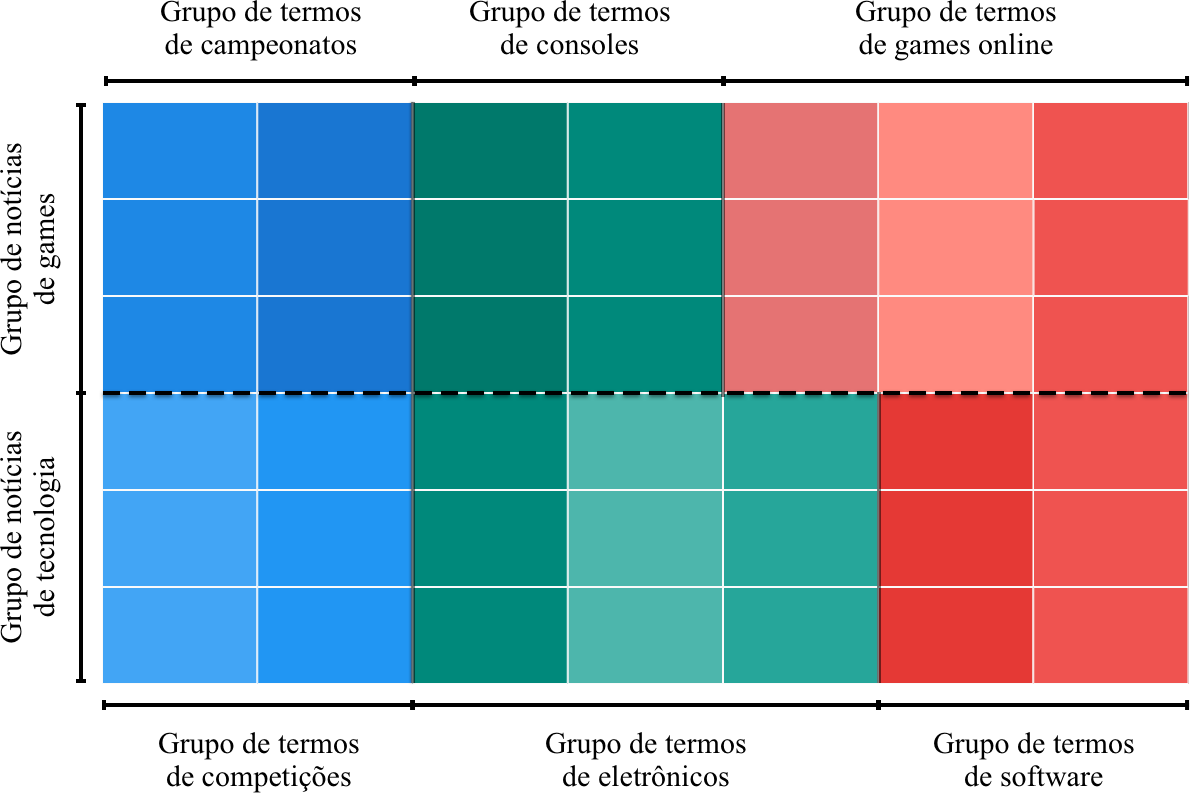
\includegraphics[width=0.7\textwidth]{img/ovnmtfNewsApplication.png}
    \label{fig:ovnmtfApplication}
\source{Lucas Fernandes Brunialti, 2016}
\end{figure}

Da mesma maneira que foi ilustrado no capítulo~\ref{ch:fatoracao} que é possível derivar interpretações intuitivas da análise das combinações de matrizes geradas na fatoração produzido pelos algoritmos lá discutidos, para os algoritmos discutidos no presente capítulo, interpretações análogas podem ser feitas, porém, consirando a existências das várias matrizes $V$.
Assumindo novamente que uma matriz de entrada representação a relação ``documento por palavras'' (linhas por colunas), cada coluna das $k$ matrizes $U I_{(p)} S, \forall p = {1, \dots, k}$, captura a ideia de uma base para representação de grupos de palavras, descritos nas matrizes $V_{(p)}$; e cada linha em $\sum_{p=1}^k S V_{(p)}^T$, captura a ideia de uma base de representação de grupos de documentos.
A representação gráfica para o resultado de uma fatoração de matrizes que permite esse raciocínio é apresentada na figura~\ref{fig:factorizationXUSV1tok}.

\begin{figure}[H]
\centering
    \caption{
        Fatoração da matriz original de dados $X$ em cinco outras matrizes: $U$, $S$, $V_1$, $V_2$ e $V_3$}
    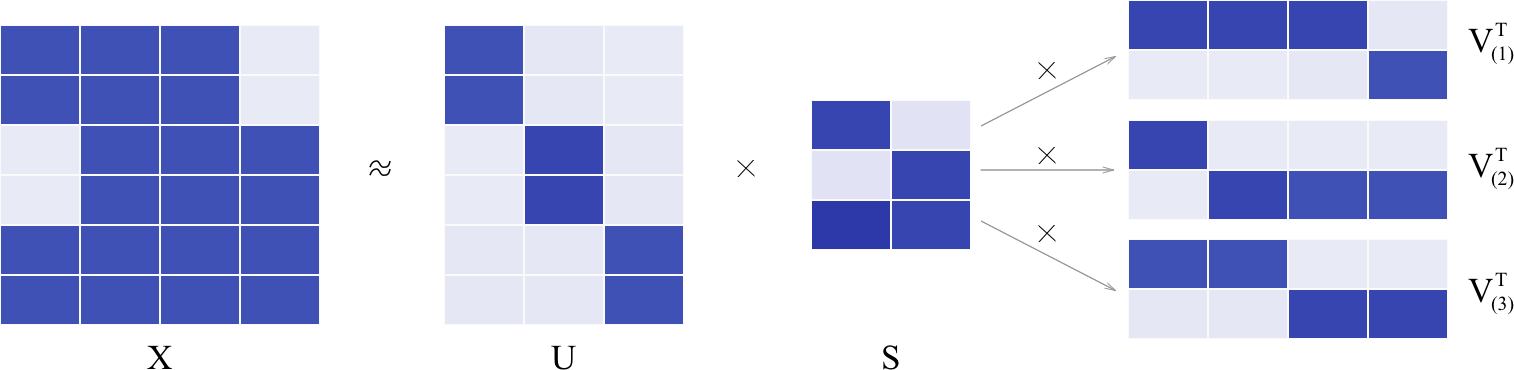
\includegraphics[width=0.8\textwidth]{img/factorizationXUSV1tok.png}
    \label{fig:factorizationXUSV1tok}
\source{Lucas Fernandes Brunialti, 2016}
\end{figure}

Todo o universo de interpretações delineado para os algoritmos da literatura podem ser estendidos para esse novo contexto de problema de agrupamento.
No entanto, agora existem três matrizes para determinar os grupos de palavras, cada uma delas responsável por determinar os grupos de palavras para cada grupo de documentos.
Na figura~\ref{fig:factorizationXUSV1tok} considere que uma célula com cor escura representa a existência de uma relação entre linha e coluna, e uma célula com cor clara representa a inexistência de uma relação entre linha e coluna, e que essas relações são estabelecidas adequadamente em cada contexto de aplicação.
Tem-se então, um conjunto de seis documentos e quatro palavras.
A matriz $U$ pode ser interpretada como descrito anteriormente, uma matriz ``documentos por grupos de documentos'', com seis documentos agrupados em três grupos ($k = 3$): os dois primeiros documentos no primeiro grupo, os dois próximos no segundo grupo e os dois últimos no terceiro grupo.
Já as matrizes $V_{(p)}^T$ têm uma interpretação levemente diferente, ainda podem ser interpretadas como matrizes de ``grupos de palavras por palavras'', sendo dois grupos de palavras ($l = 2$), porém, a matriz $V_{(1)}^T$, por exemplo, contém os grupos de palavras para o primeiro grupo de documentos apenas (composto pelas linhas $1$ e $2$ de $X$), no primeiro grupo de palavras estão as colunas $1$, $2$ e $3$, e no segundo, a coluna $4$.
O mesmo raciocínio pode ser utilizado para as matrizes $V_{(2)}^T$ e $V_{(3)}^T$.
Por fim, para a matriz $S$ pode ser realizada a mesma interpretação, representando uma relação entre grupos de documentos e grupos de palavras, com a ressalva de que irão existir $k \times l$ grupos de palavras, ou seja, a linha $p$ da matriz $S$ irá representar a relação entre o $p$-ésimo grupo de documentos e os grupos de palavras encontrados em $V_{(p)}^T$.

O restante deste capítulo é destinado a apresentar a formulação dos problemas para cada uma das estratégias, incluindo a apresentação de uma derivação teórica para um algoritmo que implementa o processo de resolução para os problemas.
Finalmente, as considerações finais apresentam uma discussão sobre o diferencial dessas estratégias no que diz respeito aos três aspectos citados no início do capítulo.

% OvNMTF
    % Explicação -> Figura, novo significado da matriz
    % Problema
    % Solução
        % - derivação
        % - algoritmo
        % - prova (?)

\section{Fatoração Tripla de Matrizes Não-negativas com Sobreposição Unidimensional}

Baseado no problema~\ref{def:bvd:problem}~\cite{Long2005}, o problema~\ref{def:ovnmtf:problem} é apresentado neste trabalho, e recebe aqui o nome de Fatoração Tripla de Matrizes Não-negativas Sobrepostas (Overlapped Non-negative Matrix Tri-factorization - OvNMTF).

\begin{problem}[Problema de Fatoração Tripla de Matrizes Não-negativas Sobrepostas]
\label{def:ovnmtf:problem}
\begin{equation}
    \begin{array}{lclc}
        \displaystyle \mathcal{F}_4(U, S, V_{(1)}, \dots, V_{(k)}) & = & \displaystyle \min_{U, S, V_{(1)}, \dots, V_{(k)}} & \norm{X - U\sum_{p=1}^{k}I_{(p)}SV_{(p)}^T}^{2}_{F} \\
                                                                   &   & \text{suj. a}                & U \geq 0, S \geq 0, \\
                                                                   &   &                              & V_{(p)} \geq 0, \quad \forall p
    \end{array} \nonumber
\end{equation}
\end{problem}

em que $U \in \mathbb{R}^{n \times k}_{+}$, $S \in \mathbb{R}^{k \times l}_{+}$, $V_{(p)} \in \mathbb{R}^{m \times l}_{+}$, $p = \{1, \dots, k\}$ é o índice para o conjunto de matrizes $\{ V_{(1)}, \dots, V_{(k)} \}$, $I_{(p)} \in \{0,1\}^{k \times k}$ é uma matriz identidade seletora, e $\norm{\cdot}_F$ denota a norma de Frobenius.
Na formulação, o papel das matrizes $I_k$ seletoras é, justamente, organizar a base de grupos de linhas, de forma que cada um deles seja otimizado de acordo com uma das matrizes $V_k$.

É possível perceber, que neste caso, diferente dos apresentados no capítulo~\ref{ch:fatoracao}, têm menor capacidade de compactação, porém, com maior nível de detalhamento.
Isso se explica, pois a partir dos $nm$ elementos da matriz de dados, são gerados $nk + kl + klm$ para representá-los, diferente.

Desde que o problema~\ref{def:ovnmtf:problem} é semelhante ao problema~\ref{def:onmtf:problem}, é esperado que ele possa também ser resolvido por meio de regras de atualização multiplicativas.
Assim, seguindo o exposto em~\cite{Yoo2010}, a derivação das regras é aqui apresentada por meio de um abordagem baseada no cálculo do gradiente.
Contudo, para o cálculo do gradiente de $\mathcal{F}_4$ a estratégia usada aqui é a apresentada em~\citeonline{Yoo2010}, de forma que $\nabla \mathcal{F}_4 = [\nabla \mathcal{F}_4]^+ - [\nabla \mathcal{F}_4]^-$.\blfootnote{Considere as seguintes igualdades para o cálculo dos gradientes, sendo $A, Q, B$ e $C$ matrizes de quaisquers dimensões adequadas para a realização das multiplicações:
\begin{equation}
\label{eq:diff:AQB}
    \begin{array}{lcl}
        \nabla_Q tr( AQB )     & = & A^T B^T \\
        \nabla_{Q^T} tr( AQB ) & = & BA \\
    \end{array}
\end{equation}

\begin{equation}
\label{eq:diff:AQBQtC}
    \begin{array}{lcl}
        \nabla_Q tr( AQBQ^TC )     & = & A^TC^TQB^T + CAQB \\
        \nabla_{Q^T} tr( AQBQ^TC ) & = & BQ^TCA + B^TQ^TA^TC^T
    \end{array}
\end{equation}
}

Expandindo $\mathcal{F}_4$, com base nas propriedade de traço de matrizes, para tornar o cálculo do gradiente mais simples, é possível obter:
\[
    \begin{array}{lcl}
        \displaystyle \mathcal{F}_4 & = & tr\big[ (X - U\sum_{p=1}^{k}I_{(p)}SV_{(p)}^T)^T (U\sum_{p=1}^{k}I_{(p)}SV_{(p)}^T) \big] \\
                                    & = & tr(X^TX) - 2 tr( X^T U \sum_{p=1}^{k} I_{(p)} S V_{(p)}^T ) + tr( \sum_{p=1}^{k} V_{(p)} S^T I_{(p)} U^T U \sum_{p'=1}^k I_{(p')} S V_{(p')}^T )
    \end{array}
\]

Note que a matriz seletora tem a seguinte propriedade: $I_{(p)}^T = I_{(p)}$.

Para o cálculo de $\nabla_U \mathcal{F}_4$, considere as partes positiva e negativa desse gradiente, $[\nabla_U \mathcal{F}_4]^+$ e $[\nabla_U \mathcal{F}_4]^-$, respectivamente.
Usando a igualdade da equação~\ref{eq:diff:AQB}, com $A = X^T$, $B = \sum_{p=1}^{k}I_{(p)}SV_{(p)}^T$ e $Q = U$, é possível obter $[\nabla_U \mathcal{F}_4]^-$, como segue.
\[
    \begin{array}{lcl}
        [\nabla_U \mathcal{F}_4]^- & = & - 2 \nabla_U \Big( tr\big[ X^T U \sum_{p=1}^{k}I_{(p)}SV_{(p)}^T \big] \Big) \\
                                   & = & - 2 X \sum_{p=1}^{k} V_{(p)} S^T I_{(p)}
    \end{array}
\]

Para o cálculo de $[\nabla_U \mathcal{F}_4]^+$, é utilizado a igualdade da equação~\ref{eq:diff:AQBQtC}, com $A = \sum_{p=1}^{k} V_{(p)} S^T I_{(p)}$, $B = I$, $Q = U^T$ e $C = \sum_{p'=1}^{k}I_{(p')}SV_{(p')}^T$. Então tem-se
\[
    \begin{array}{lcl}
        [\nabla_U \mathcal{F}_4]^+ & = & \nabla_U \Big( tr(X^TX) + tr\big[ \sum_{p=1}^{k} V_{(p)} S^T I_{(p)} U^T U \sum_{p'=1}^k I_{(p')} S V_{(p')}^T \big] \Big) \\
                                   & = & U \sum_{p'=1}^k I_{(p')} S V_{(p')}^T \sum_{p=1}^{k} V_{(p)} S^T I_{(p)} \\
                                   &   & + ~ U \sum_{p=1}^k I_{(p)} S V_{(p)}^T \sum_{p'=1}^{k} V_{(p')} S^T I_{(p')} \\
                                   & = & 2 U \sum_{p=1}^k \sum_{p'=1}^{k} I_{(p)} S V_{(p)}^T V_{(p')} S^T I_{(p')}
    \end{array}
\]

De forma similar, para o cálculo de $\nabla_S \mathcal{F}_4$, considere as partes positiva e negativa, $[\nabla_S \mathcal{F}_4]^+$ e $[\nabla_S \mathcal{F}_4]^-$, respectivamente.
Usando a igualdade da equação~\ref{eq:diff:AQB} para todas as partes da soma de $p = 1, \dots, k$, com $A = X^T U I_{(p)}$, $Q = S$, e $B = V_{(p)}^T$, é possível obter $[\nabla_S \mathcal{F}_4]^-$, como segue:
\[
    \begin{array}{lcl}
        [\nabla_S \mathcal{F}_4]^- & = & - 2 \nabla_S \Big( tr\big[ X^T U I_{(1)}SV_{(1)}^T \big] + \dots + tr\big[ X^T U I_{(k)}SV_{(k)}^T \big] \Big) \\
                                   & = & - 2 \Big( I_{(1)} U^T X V_{(1)} + \dots + I_{(k)} U^T X V_{(k)} \Big) \\
                                   & = & - 2 \sum_{p=1}^{k} I_{(p)} U^T X V_{(p)}
    \end{array}
\]

Para o cálculo de $[\nabla_S \mathcal{F}_4]^+$, é utilizado a igualdade da equação~\ref{eq:diff:AQBQtC} para todas as partes da soma de $p = p' = 1, \dots, k$, com $A = V_{(p)}$, $Q = S^T$, $B = I_{(p)} U^T U I_{(p')}$ e $C = V_{(p')}^T$. Então tem-se
\[
    \begin{array}{lcl}
        [\nabla_S \mathcal{F}_4]^+ & = & \nabla_S \Big( tr(X^TX) + tr\big[ V_{(1)} S^T I_{(1)} U^T U I_{(1)} S V_{(1)}^T \big] + \dots + tr\big[ V_{(1)} S^T I_{(1)} U^T U I_{(k)} S V_{(k)}^T \big]  \\
                                   &   & + \dots + tr\big[ V_{(k)} S^T I_{(k)} U^T U I_{(1)} S V_{(1)}^T \big] + \dots + tr\big[ V_{(k)} S^T I_{(k)} U^T U I_{(k)} S V_{(k)}^T \big] \Big) \\
                                   & = & \big( I_{(1)} U^T U I_{(1)} S V_{(1)}^T V_{(1)} + I_{(1)} U^T U I_{(1)} S V_{(1)}^T V_{(1)} \big) \\
                                   &   & + \dots + \big( I_{(1)} U^T U I_{(k)} S V_{(k)}^T V_{(1)} + I_{(k)} U^T U I_{(1)} S V_{(1)}^T V_{(k)} \big) \\
                                   &   & + \dots + \big( I_{(k)} U^T U I_{(1)} S V_{(1)}^T V_{(k)} + I_{(1)} U^T U I_{(k)} S V_{(k)}^T V_{(1)} \big) \\
                                   &   & + \dots + \big( I_{(k)} U^T U I_{(k)} S V_{(k)}^T V_{(k)} + I_{(k)} U^T U I_{(k)} S V_{(k)}^T V_{(k)} \big) \\
                                   & = & 2 \sum_{p=1}^{k} \sum_{p'=1}^{k} I_{(p)} U^T U I_{(p')} S V_{(p')}^T V_{(p)}
    \end{array}
\]


Finalmente, para o cálculo de $\nabla_{V_{(p)}} \mathcal{F}_4$, considere as partes positiva e negativa, $[\nabla_{V_{(p)}} \mathcal{F}_4]^+$ e $[\nabla_{V_{(p)}} \mathcal{F}_4]^-$, respectivamente. Usando a igualdade da equação~\ref{eq:diff:AQB}, com $A = X^T U I_{(p)} S$, $Q = V^{T}_{(p)}$, e $B = I$, $\forall p$, é possível obter $[\nabla_{V_{(p)}} \mathcal{F}_4]^-$, da seguinte forma:
\[
    \begin{array}{lcl}
        [\nabla_{V_{(p)}} \mathcal{F}_4]^- & = & - 2 \nabla_{V_{(p)}} \Big( tr\big[ X^T U I_{(1)}SV_{(1)}^T \big] + \dots + tr\big[ X^T U I_{(k)}SV_{(k)}^T \big] \Big) \\
                                           & = & - 2 X^T U I_{(p)} S
    \end{array}
\]

Fixando a derivação para $[\nabla_{V_{(p)}} \mathcal{F}_4]^+$ é nota-se que há dois casos diferentes para a derivação. O caso em que $p = p'$ e o caso em que $p \neq p'$. Para o caso em que $p = p'$, é utilizada a igualdade da equação~\ref{eq:diff:AQBQtC}, com $A = I$, $Q = V_{(p)}$, $B = S^T I_{(p)} U^T U I_{(p')} S$ e $C = I$, $\forall p, p'$, de forma que
\[
    \begin{array}{lcl}
        [\nabla_{V_{(p)}} \mathcal{F}_4]^{+}_{p=p'} & = & \nabla_{V_{(p)}} \Big( tr\big[ V_{(1)} S^T I_{(1)} U^T U I_{(1)} S V_{(1)}^T \big] + \dots + tr\big[ V_{(k)} S^T I_{(k)} U^T U I_{(k)} S V_{(k)}^T \big] \Big) \\
                                                    & = & \nabla_{V_{(p)}} \Big( tr\big[ V_{(p)} S^T I_{(p)} U^T U I_{(p)} S V_{(p)}^T \big] \Big)  \\
                                                    & = & 2 V_{(p)} S^T I_{(p)} U^T U I_{(p)} S
    \end{array}
\]

Para o caso em que $p \neq p'$, é usada a igualdade da equação~\ref{eq:diff:AQB} em duas outras situações, aquela em que $V_{(p)}$ esta localizado à esquerda, então, $Q = V_{(p)}$, $A = I$ e $B = S^T I_{(p)} U^T U I_{(p')}$; e aquela em que $V_{(p)}$ esta localizado à direita, então, $Q = V_{(p)}^T$, $A = V_{(p')} S^T I_{(p')} U^T U I_{(p)} S V_{(p)}^T$, $\forall p, p'$. Assim,
\[
    \begin{array}{lcl}
        [\nabla_{V_{(p)}} \mathcal{F}_4]^{+}_{p \neq p'} & = & \nabla_{V_{(p)}} \Big( tr\big[ V_{(1)} S^T I_{(1)} U^T U I_{(2)} S V_{(2)}^T \big] + \dots + tr\big[ V_{(1)} S^T I_{(1)} U^T U I_{(k)} S V_{(k)}^T \big] \\
                                   &   & + \dots + tr\big[ V_{(k)} S^T I_{(k)} U^T U I_{(1)} S V_{(1)}^T \big] + \dots + tr\big[ V_{(k)} S^T I_{(k)} U^T U I_{(k-1)} S V_{(k-1)}^T \big] \Big) \\
                                   & = & \sum_{p' \neq p} \bigg[ \nabla_{V_{(p)}} \Big( tr\big[ V_{(p)} S^T I_{(p)} U^T U I_{(p')} S V_{(p')}^T \big] \Big) \\
                                   &   & + ~ \nabla_{V_{(p)}} \Big( tr\big[ V_{(p')} S^T I_{(p')} U^T U I_{(p)} S V_{(p)}^T \big] \Big) \bigg] \\
                                   & = & \sum_{p' \neq p} 2 \big( V_{(p')} S^T I_{(p')} U^T U I_{(p)} S \big)
    \end{array}
\]

Então, é possível calcular $[\nabla_{V_{(p)}} \mathcal{F}_4]^{+}$, $\forall p$, fazendo:
\[
    \begin{array}{lcl}
        [\nabla_{V_{(p)}} \mathcal{F}_4]^{+} & = & [\nabla_{V_{(p)}} \mathcal{F}_4]^{+}_{p = p'} + [\nabla_{V_{(p)}} \mathcal{F}_4]^{+}_{p \neq p'} \\
                                             & = & 2 \big( V_{(p)} S^T I_{(p)} U^T U I_{(p)} S + \sum_{p' \neq p} V_{(p')} S^T I_{(p')} U^T U I_{(p)} S \big) \\
                                             & = & 2 \big( \sum_{p'=1}^{k} V_{(p')} S^T I_{(p')} U^T U I_{(p)} S \big)
    \end{array}
\]

O resultado final dos gradientes para $U, S, V_{(p)}, \forall, p \in \{1, \dots, k\}$ são apresentados nas equações~\ref{eq:ovnmtf:gradU},~\ref{eq:ovnmtf:gradS} e~\ref{eq:ovnmtf:gradV}, respectivamente.
\begin{equation}
\label{eq:ovnmtf:gradU}
    \begin{array}{lcl}
        \nabla_U \mathcal{F}_4 & = & 2 \big( - X \sum_{p=1}^{k} V_{(p)} S^T I_{(p)} + U \sum_{p=1}^k \sum_{p'=1}^{k} I_{(p)} S V_{(p)}^T V_{(p')} S^T I_{(p')} \big)
    \end{array}
\end{equation}
\begin{equation}
\label{eq:ovnmtf:gradS}
    \begin{array}{lcl}
        \nabla_S \mathcal{F}_4 & = & 2 \big( - \sum_{p=1}^{k} I_{(p)} U^T X V_{(p)} + \sum_{p=1}^{k} \sum_{p'=1}^{k} I_{(p)} U^T U I_{(p')} S V_{(p')}^T V_{(p)} \big)
    \end{array}
\end{equation}
\begin{equation}
\label{eq:ovnmtf:gradV}
    \begin{array}{lcl}
        \nabla_{V_{(p)}} \mathcal{F}_4 & = & 2 \big( -X^T U I_{(p)} S + \sum_{p'=1}^{k} V_{(p')} S^T I_{(p')} U^T U I_{(p)} S \big)
    \end{array}
\end{equation}

Sendo assim, as regras de atualização para as matrizes $U, V_{(p)}, S \forall p \in \{1, \dots, k\}$, são mostradas nas equações~\ref{eq:ovnmtf:updateU},~\ref{eq:ovnmtf:updateV} e~\ref{eq:ovnmtf:updateS}, apresentadas no algoritmo~\ref{algo:ovnmtf}, o qual implementa o processo de minimização para o problema~\ref{def:ovnmtf:problem}.
Nesse algoritmo $t$ é o contador de iterações, $U^{(t)}$, $S^{(t)}$ e $V_{(p)}^{(t)}$ são as matrizes $U$, $S$ e $V_{(p)}$, na iteração $t$, respectivamente, $\mathcal{U}(0, 1) \in~]0, 1]$ uma função que gera valores de uma distribuição uniforme que ignora zeros, e $\odot$ é o produto de Hadamard.

% TODO: condições de convergência não foram provadas, mas podemos dar algum insight sobre isso?

\begin{algorithm}[H]
\caption{Algoritmo baseado em atualização multiplicativa para solução do OvNMTF}
\label{algo:ovnmtf}
    \begin{algorithmic}[1]
        \Function{OvNMTF}{$X$, $t_{max}$}
            \State \textbf{Inicialize:} $U^{(0)} \geq \mathcal{U}(0,1), S^{(0)} \geq \mathcal{U}(0,1), V_{(p)}^{(0)} \geq \mathcal{U}(0,1), \forall p$ e $t \gets 0$.
            \While{(não convergiu) ou ($t \leq t_{max}$)} %\Comment{We have the answer if r is 0}
                \State
                    \begin{equation}
                    \label{eq:ovnmtf:updateU}
                        U^{(t+1)} \gets U^{(t)} \odot \frac{ \sum_{p=1}^{k} X V^{(t)}_{(p)} S^{(t)^T} I_{(p)} }{ \sum_{p=1}^{k} \sum_{p'=1}^k U^{(t)} I_{(p)} S^{(t)} V^{(t)^T}_{(p)} V^{(t)}_{(p')} S^{(t)^T} I_{(p')} }
                    \end{equation}
                \For{$p \leftarrow 1, k$}
                    \State
                        \begin{equation}
                        \label{eq:ovnmtf:updateV}
                            V^{(t+1)}_{(p)} \gets V^{(t)}_{(p)} \odot \frac{ X^T U^{(t+1)} I_{(p)} S^{(t)} }{ \sum_{p'=1}^{k} V_{(p')} S^T I_{(p')} U^T U I_{(p)} S }
                        \end{equation}
                \EndFor
                \State
                    \begin{equation}
                    \label{eq:ovnmtf:updateS}
                        S^{(t+1)} \gets S^{(t)} \odot \frac{ \sum_{p=1}^{k} I_{(p)} U^{(t+1)^T} X V^{(t+1)}_{(p)} }{ \sum_{p=1}^{k} \sum_{p'=1}^{k} I_{(p)} U^{(t+1)^T} U^{(t+1)} I_{(p')} S^{(t)} V^{(t+1)^T}_{(p')} V^{(t+1)}_{(p)} }
                    \end{equation}
                \State $t \gets t + 1$
            \EndWhile\label{euclidendwhile}
            \State \textbf{return} $U^{(t)}, S^{(t)}, V_{(1)}^{(t)}, \dots, V_{(k)}^{(t)}$
        \EndFunction
    \end{algorithmic}
\end{algorithm}

A inicialização dos elementos das matrizes $U$, $S$ e $V_{(1)}, \dots, V_{(k)}$ são gerados através de uma distribuição uniforme que ignora zeros ($\mathcal{U}(0, 1) \in~]0, 1]$).
Como condições para assumir a convergência, assim como os algoritmos apresentados no capítulo~\ref{ch:fatoracao}, considera-se a diferença do erro de aproximação em duas iterações consecutivas menor ou igual a um $\epsilon$:
$$\norm{X - U^{(t)} \sum_{p=1}^k I_{(p)} S^{(t)} V^{(t)^T}_{(p)} }^{2}_{F} - \norm{X - U^{(t+1)} \sum_{p=1}^k I_{(p)} S^{(t+1)} V^{(t+1)^T}_{(p)} }^{2}_{F} \leq \epsilon$$
O algoritmo também pára caso a $t$-ésima iteração seja igual ao número máximo de iterações ($t_{max}$).

O particionamento, neste caso, não é direto.
Então é necessário um processo de pós-processamento para a matriz $U$ e para as matrizes $V_{(1)}, \dots, V_{(k)}$.
Um modo simples de obter o particionamento para as linhas, já descrito no capítulo~\ref{ch:fatoracao}, é o seguinte:
\[
    \mathcal{K}_p = \mathcal{K}_p + \{ x_{i \cdot} \}~|~p = \argmax_{p'} \mathbf{u}_{i \cdot}~\forall i = \{1, \dots, n\}, \forall p, p' = \{1, \dots, k\}
\]

Pode-se usar a mesma estratégia para o particionamento das colunas:
\[
    \mathcal{L}_{pq} = \mathcal{L}_{pq} + \{ x_{\cdot j} \}~|~q = \argmax_{q'} \mathbf{v}_{(p)_{j \cdot}}~\forall j = \{1, \dots, m\}, \forall q, q' = \{1, \dots, l\}, \forall p = \{1, \dots, k\}
\]

\section{Fatoração Binária Tripla de Matrizes Não-negativas com Sobreposição Unilateral}

% BinOvNMTF
    % Explicação
    % Problema
    % Solução
        % - derivação
        % - algoritmo
        % - prova (?)

A segunda estratégia proposta nesta dissertação, segue os pressupostos estabelecidos por~\citeonline{Wang2011} no problema~\ref{def:fnmtf:problem}.
O problema~\ref{def:binovnmtf:problem}, então denominado Fatoração Binária Tripla de Matrizes Não-negativas com Sobreposição Unilateral (Unilateral Overlapped Binary Non-negative Matrix Tri-factorization - BinOvNMTF) também está associado a diminuição da flexibilidade da solução de coagrupamento apresentada no que diz respeito à relação de associação entre grupos de linhas e grupos de colunas, a qual aqui é binária.
Porém, mantém a independência do estabelecimento de diferentes bases para os grupos de linhas, uma vez que também assume a existência de $k$ matrizes $V$.

\begin{problem}[Problema de Fatoração Binária Tripla de Matrizes Não-negativas Sobrepostas]
\label{def:binovnmtf:problem}
\begin{equation}
    \begin{array}{lclc}
        \displaystyle \mathcal{F}_5(U, S, V_{(1)}, \dots, V_{(k)}) & = & \displaystyle \min_{U, S, V_{(1)}, \dots, V_{(k)}} & \norm{ X - U \sum_{p=1}^{k} I_{(p)} S V_{(p)}^T }^{2}_{F} \\
                                                                   &   & \text{suj. a}                & U \in \Psi^{n \times k}, \\
                                                                   &   &                              & V_{(p)} \in \Psi^{m \times l}, \quad \forall p
    \end{array}   \nonumber
\end{equation}
\end{problem}

em que $\Psi = \{0, 1\}$, $\sum_{p=1}^{k} \mathbf{u}_{p \cdot} = 1$ e $\sum_{q=1}^{l} \mathbf{v}_{(p)_{q \cdot}} = 1, \forall p$, $p = \{1, \dots, k\}$ e $q = \{1, \dots, l\}$ são os índices que iteram no número de linhas e colunas, respectivamente, $I_{(p)} \in \{0,1\}^{k \times k}$ é uma matriz identidade seletora, e $\norm{\cdot}_F$ denota a norma de Frobenius para matrizes.
Ainda, as restrições $\sum_{p=1}^{k} \mathbf{u}_{p \cdot} = 1$ e $\sum_{q=1}^{l} \mathbf{v}_{(p)_{q \cdot}} = 1, \forall p$ garantem que uma linha e uma coluna de um grupo, respectivamente, têm que pertencer à algum grupo.

Em termos de compactação, a interpretação é semelhante à interpretação feita para o problema~\ref{def:ovnmtf:problem}, porém, por causa das restrições serem binárias, os $nm$ elementos da matriz de dados serão compactados em $n + kl + km$ elementos.

A mesma estratégia de derivação utilizada no algoritmo~\ref{algo:fnmtf}, também pode ser feita para propor uma solução para o problema~\ref{def:binovnmtf:problem}: solucionar o problema para $S$ para obter subproblemas que podem ser solucionados através de uma estratégia iterativa.
Então, recapitulando o gradiente $[\nabla_S \mathcal{F}_4]^+$, já calculado para solução do problema~\ref{def:ovnmtf:problem}, será o mesmo para $\mathcal{F}_5$, porém passível de simplificação, como $(U^T U)$, para o problema~\ref{def:binovnmtf:problem} que tem restrições binárias em $U$, é uma matriz que contém zeros em todos elementos, com exceção da diagonal principal:
\[
    \begin{array}{lcl}
        [\nabla_S \mathcal{F}_5]^+ & = & \sum_{p=1}^{k} \sum_{p'=1}^{k} I_{(p)} U^T U I_{(p')} S V_{(p')}^T V_{(p)} \\
                                   & = & \sum_{p=1}^{k} \sum_{p'=1}^{k} \Bigg( I_{(p)}
                                   \begin{bmatrix}
                                       (U^T U)_{11}            &        & \smash{\text{\large 0}} \\
                                                               & \ddots &                         \\
                                       \smash{\text{\large 0}} &        & (U^T U)_{kk}
                                   \end{bmatrix} I_{(p')} \Bigg) S V_{(p')}^T V_{(p)}
    \end{array} \nonumber
\]

Note que se $p \neq p'$, $I_{(p)} U^T U I_{(p)}$ e toda expressão, será uma matriz de zeros, por exemplo, se $p=1$ e $p'=2$:
\[
\begin{array}{lcl}
    I_{(1)}
    \begin{bmatrix}
        (U^T U)_{11}            &        & \smash{\text{\large 0}} \\
                                & \ddots &                         \\
        \smash{\text{\large 0}} &        & (U^T U)_{kk}
    \end{bmatrix}
    I_{(2)}
    & = & \begin{bmatrix}
          1      & \hdots & 0      \\
          \vdots & \ddots & \vdots \\
          0      & \hdots & 0
      \end{bmatrix}
      \begin{bmatrix}
          (U^T U)_{11}            &        & \smash{\text{\large 0}} \\
                                  & \ddots &                         \\
          \smash{\text{\large 0}} &        & (U^T U)_{kk}
      \end{bmatrix}
      \begin{bmatrix}
          0      & \hdots & 0      \\
          0      &    1   & 0      \\
          \vdots & \ddots & \vdots \\
          0      & \hdots & 0
      \end{bmatrix} \\
      & = & (0)_{kk}
\end{array}
\]
\[
    \begin{array}{lclcl}
        \therefore & [\nabla_S \mathcal{F}_5]^+ & = & \sum_{p=1}^{k} I_{(p)} U^T U I_{(p)} S V_{(p)}^T V_{(p)}
    \end{array}
\]

Assim, é possível escrever o gradiente $\nabla_S \mathcal{F}_5$, a fim de encontrar uma expressão para atualização de $S$.
\[
    \begin{array}{lcl}
        [\nabla_S \mathcal{F}_5]^+ &     =    & - 2 \sum_{p=1}^{k} I_{(p)} U^T X V_{(p)} + 2 \sum_{p=1}^{k} I_{(p)} U^T U I_{(p)} S V_{(p)}^T V_{(p)} = 0 \\
                                   & \implies & \sum_{p=1}^{k} I_{(p)} U^T U I_{(p)} S V_{(p)}^T V_{(p)} = \sum_{p=1}^{k} I_{(p)} U^T X V_{(p)}
    \end{array}   \nonumber
\]

Como os termos $I_{(p)} U^T X V_{(p)}$ e $I_{(p)} U^T U I_{(p)} S V_{(p)}^T V_{(p)}$, $\forall p$, por serem multiplicados por $I_{(p)}$ pela esquerda, correspondem a cada linha da matriz que será a atualização de $S$, aqui denotado por $\widetilde{S} = I_{(p)} S$.
Observe que $I_{(p)} (U^T U)^{-1} I_{(p)} = I_{(p)} (U^T U)^{-1}$, dado a estrutura de $(U^T U)$.
\[
    \begin{array}{lcl}
        I_{(p)} U^T U \widetilde{S} V_{(p)}^T V_{(p)} & = & I_{(p)} U^T X V_{(p)} \\
        \widetilde{S}                                 & = & I_{(p)} (U^T U)^{-1} I_{(p)} U^T X V_{(p)} V_{(p)}^T V_{(p)} \\
                                                      & = & I_{(p)} (U^T U)^{-1} U^T X V_{(p)} V_{(p)}^T V_{(p)}
    \end{array}
\]

\[
    \therefore ~ S = \sum_{p=1}^k I_{(p)} (U^T U)^{-1} U^T X V_{(p)} V_{(p)}^T V_{(p)}
\]

É importante ressaltar que a mesma interpretação realizada para atualização de $S$ no algoritmo~\ref{algo:fnmtf}, também é possível ser transferida para esse contexto.

Assim, é possível transformar o problema~\ref{def:binovnmtf:problem} em subproblemas para atualização de $U$ e $V_{(1)}, \dots, V_{(k)}$.
Usando a mesma estratégia iterativa adotada no algoritmo~\ref{algo:fnmtf}: obtém-se os protótipos de linhas e verifica-se quais linhas de $X$ mais se aproximam de cada um dos protótipos, para atualização de $U$; então, é feito o mesmo processo para atualização de $V_{(1)}, \dots, V_{(k)}$, obtém-se os protótipos de colunas, relativo à $V_{(p)}, \forall p$, e verifica-se quais colunas de $X$ mais se aproximam de cada um dos protótipos.

O implementação desse processo é apresentado no algoritmo~\ref{algo:binovbnmtf}).
Considere $t$ o contador de iterações, $U^{(t)}$, $S^{(t)}$ e $V_{(p)}^{(t)}$ são as matrizes $U$, $S$ e $V_{(p)}$, na iteração $t$, respectivamente, $\mathcal{U}(0, 1) \in~]0, 1]$ uma função que gera valores de uma distribuição uniforme que ignora zeros, e $\norm{ \cdot }^2$ é a norma frobenius para vetores.

\begin{algorithm}
\caption{Algoritmo iterativo para solução do BinOvNMTF}
\label{algo:binovbnmtf}
    \begin{algorithmic}[1]
        \Function{BinOvNMTF}{$X$, $t_{max}$, $k$, $l$}
            \State \textbf{Inicialize:} $U^{(0)} \geq 0, 1 ~|~ \sum_{p=1}^{k} \mathbf{u}_{p \cdot} = 1$, $V_{(p)}^{(0)} \geq 0, 1 ~|~\sum_{q=1}^{l} \mathbf{v}_{(p)_{q \cdot}} = 1, \forall p$, $S^{(0)} \gets \mathcal{U}(0, 1)$ e $t \gets 0$.
            \While{(não convergiu) ou ($t \leq t_{max}$)}
                \State
                    \begin{equation}
                    \label{eq:binovbnmtf:updateS}
                        S^{(t+1)} \gets \sum_{p=1}^k I_{(p)} (U^{(t)^T} U)^{-1} U^{(t)^T} X V_{(p)}^{(t)} (V_{(p)}^{(t)^T} V_{(p)}^{(t)})^{-1}
                    \end{equation}
                \State
                    \[
                        \widetilde{V} \gets \sum_{p=1}^k I_{(p)} S^{(t+1)} V_{(p)}^{(t)^T}
                    \]
                \State
                    \begin{equation}
                    \label{eq:binovbnmtf:updateF}
                        (U^{(t+1)})_{ip} \gets \left\{
                            \begin{array}{ll}
                                1 & p = \argmin_{p' \in \{1, \dots, k\}} \norm{ \mathbf{x}_{i \cdot} - \mathbf{\widetilde{v}}_{p' \cdot} }^2 \\
                                0 & \textit{caso contrário}
                            \end{array}
                        \right. \forall i, p
                    \end{equation}
                \State
                    \[
                        \widetilde{U}_{(p)} \gets U^{(t+1)} I_{(p)} S^{(t+1)}, \forall p
                    \]
                \State
                    \begin{equation}
                    \label{eq:binovbnmtf:updateG}
                        (V_{(p)}^{(t+1)})_{jq} \gets \left\{
                            \begin{array}{ll}
                                1 & q = \argmin_{q' \in \{1, \dots, l\}} \norm{ \mathbf{x}_{\cdot j} - \mathbf{\widetilde{u}}_{\cdot q'} }^2 \\
                                0 & \textit{caso contrário}
                            \end{array}
                        \right. \forall j, q, p
                    \end{equation}
                \State $t \gets t + 1$
            \EndWhile\label{euclidendwhile}
            \State \textbf{return} $U^{(t)}, S^{(t)}, V_{(1)}^{(t)}, \dots, V_{(k)}^{(t)}$
        \EndFunction
    \end{algorithmic}
\end{algorithm}

Note que nesse tipo de fatoração, semelhante à apresentada no problema~\ref{def:fnmtf:problem}, não necessita de uma fase de pós-processamento para obter o particionamento de linhas e colunas, pois o mesmo é direto a partir das matrizes $U$ e $V_{(1)}, \dots, V_{(k)}$.
Ainda, usa-se a mesma estratégia de convergência que a apresentada no algoritmo~\ref{algo:ovnmtf}.

\section{Considerações Finais}

A motivação para a apresentação dos novos problemas de fatoração de matrizes (OvNMTF e BinOvNMTF), era a possibilidade de superar algumas das dificuldades apresentas nas fatorações da literatura (ONMTF e FNMTF), no que diz respeito à solução do problema de coagrupamento.

Do ponto de vista de quantização do espaço dos dados, a quantidade de informação armazenada nas novas fatorações tem o potencial de superar as fatorações da literatura.
Isso ocorre porque nas fatorações propostas, o número de colunas $l$ necessários para explicar a matriz de dados original deve ser mais próxima daquele necessário para obter o número de grupos de colunas desejado, mesmo para os casos em que há interseção de colunas entre as diferentes bases dos grupos de linhas.
Entretanto, as fatorações propostas necessitam criar $k$ matrizes para a abstração dos grupos de colunas, o que incorre em um custo maior de armazenamento dos protótipos dos grupos de colunas, e portanto, menor capacidade de compactação.

Do ponto de vista de geração de informação sobre os dados, as fatorações propostas são capazes de fornecer o mesmo tipo de informação: como as linhas da matriz de entrada se organizam em grupos e como as colunas da matriz de entrada se organizam em grupo.
Porém, desde que se tem $k$ organizações de grupos de colunas, sabe-se que há várias possibilidades dessa organização ocorrer para cada um dos grupos de linhas.
Transferindo essa informação para um contexto de aplicação, entende-se que há um conjunto de organização de atributos que estão associados à organização assumida pelos dados no espaço dos dados.
Intuitivamente, pode-se dizer que há diferentes maneiras de justificar o agrupamento de dados descoberto, com base nas similaridades parciais dos atributos que os descrevem.

Do ponto de vista do processo de descoberta dos cogrupos, as fatorações propostas seguem o mesmo principio seguido nas fatorações da literatura, qual seja, considerar a informação de similaridade de dados e de atributos simultaneamente para resolver o problema de minimização do erro de quantização da matriz original, e consequentemente apresentar protótipos que expliquem os cogrupos.
Porém, as fatorações propostas liberam os algoritmos de minimização da necessidade de considerar todos os grupos de linhas na otimização dos grupos de colunas.
Desta forma, implementa-se um processo no qual não existe mais a interdependência entre grupos de linhas.
Esse fato é que, na realidade, possibilita aproximar a quantidade de cogrupos utilizada para explicar os dados daquela que é a desejada, ainda que a sobreposição de colunas ocorra nos dados.

Essa considerações, assim como aquelas delineadas nos capítulos~\ref{ch:conceitos} e~\ref{ch:fatoracao}, são ilustradas no próximo capítulo, no qual resultados experimentais são apresentados.

% ************************************************************
% ************************************************************
% ************************************************************

% \chapter{A proposta}
% \label{ch:proposta}

% \section{Overlapping Orthogonal Nonnegative Matrix Tri Factorization}

% This is a proposal algorithm that aims to solve the following problem:
% $$\mathcal{F}_1 = \textit{min } ||X - U\sum_{i=1}^{k}I^{(i)}SV^{(i)}||^{2}_{F}$$
% % $$\textit{s.t. } U^TU = I$$
% % $$\left[ \begin{array}{c} V^{(1)} \\ V^{(2)} \\ \vdots \\ V^{(k)} \end{array} \right]^T\left[ \begin{array}{c} V^{(1)} \\ V^{(2)} \\ \vdots \\ V^{(k)} \end{array} \right] = I$$
% % $$\left[ \begin{array}{c} V^{(1)} \\ V^{(2)} \\ \vdots \\ V^{(k)} \end{array} \right] \geq 0$$
% $$\textit{s.t. } U, S, V^{(1)}, \dots, V^{(k)} \geq 0$$

% where $X \in \mathbb{R}^{n \times m}$ a data matrix, $U \in \mathbb{R}^{n \times k}$ an matrix containing rows clusters, $I^{(i)} \in \mathbb{R}^{k \times k}$ an indicator matrix, $S \in \mathbb{R}^{k \times l}$ a block matrix, $V^{(i)} \in \mathbb{R}^{l \times m} \forall i \in \{1, \dots, k\}$ matrices containing columns clusters for each row cluster, and $||\cdot||^2_{F}$ denotes the frobenius norm.


% Consider the lagrange function:
% $$\mathcal{L} = \mathcal{F}_1 - tr(\Lambda_1 U^T) - tr(\Lambda_2 S^T) - \sum_{i=1}^{k} tr(A_i V^{(i)^T})$$

% where $\Lambda_1, \Lambda_2$ and $A_i \forall i \in \{1, \dots, k\}$ are lagrange multipliers: $\Lambda_1 \in \mathbb{R}^{n \times k}$, $\Lambda_1 \in \mathbb{R}^{k \times l}$, and $A_i \in \mathbb{R}^{k \times l} \forall i \in \{1, \dots, k\}$.

% KKT Conditions:
% \begin{itemize}
% \item $\frac{\partial \mathcal{L}}{\partial U} = 0$
% \item $\frac{\partial \mathcal{L}}{\partial S} = 0$
% \item $\frac{\partial \mathcal{L}}{\partial V^{(i)}} = 0, \forall i \in \{1, \dots, k\}$
% \item $\Lambda_1 \odot U = 0$
% \item $\Lambda_2 \odot S = 0$
% \item $A_i \odot V^{(i)} = 0, \forall i \in \{1, \dots, k\}$
% \end{itemize}
% %\paragraph{}
% where $\odot$ denotes the element-wise multiplication.

% Given that:
% $$\frac{\partial}{\partial B} tr \left[ (RBC + D)(RBC + D)^T \right] = 2R^T(RBC + D)C^T = 2R^trBCC^T + 2R^TDC^T$$

% It is possible to calculate $\frac{\partial \mathcal{L}}{\partial U}$, considering $R = -I, B = U, C = \sum I^{(i)}SV^{(i)}, D = X$:
% $$\frac{\partial \mathcal{L}}{\partial U} = 2 U \sum_{i=1}^k I^{(i)} S V^{(i)} \sum_{j=1}^k V^{(j)^T} S^T I^{(j)} - 2 X \sum_{i=1}^k V^{(i)^T} S^T I^{(i)} - \Lambda_1$$

% For $\frac{\partial \mathcal{L}}{\partial V}$, consider $R = U \sum I^{(i)} S, B = V^{(i)}, C = -I, D = X$:
% $$\frac{\partial \mathcal{L}}{\partial V^{(j)}} = 2 S^T I^{(j)} U^T U I^{(j)} S V^{(j)} - 2 S^T I^{(j)}  U^T X - A_j, \forall j \in \{1, \dots, k\}$$

% For $\frac{\partial \mathcal{L}}{\partial S}$, consider that $\frac{\partial (A X B X^T C)}{\partial X} = A^T C^T X B^T + C A X B$:
% $$\frac{\partial \mathcal{L}}{\partial S} = \frac{\partial}{\partial S} tr (X - U \sum_{i=1}^{k} I^{(i)} S V^{(i)}) (U \sum_{j=1}^{k} I^{(j)} S V^{(j)})^T   - tr(\Lambda_2 S^T)$$

% $$= \frac{\partial}{\partial S} tr(X^TX) - 2 \frac{\partial}{\partial S} tr(X U \sum_{i=1}^{k} I^{(i)} S V^{(i)}) + tr(\sum_{j=1}^k \sum_{i=1}^k U I^{(i)} S V^{(i)} V^{(j)^T} S^T I^{(j)} U^T ) - tr(\Lambda_2 S^T)$$

% $$= -2 \sum_{i=1}^{k} I^{(i)} U^T X^T V^{(i)^T} + \sum_{i=1}^{k} \sum_{j=1}^{k} [ I^{(i)} U^T U I^{(j)} S V^{(j)} V^{(i)^T} +  I^{(j)} U^T U I^{(i)} S V^{(i)} V^{(j)^T} ]$$

% $$= -2 \sum_{i=1}^{k} I^{(i)} U^T X^T V^{(i)^T} + \sum_{i=1}^{k} \sum_{j=1}^{k} I^{(i)} U^T U I^{(j)} S V^{(j)} V^{(i)^T}$$


% ************************************************************
% ************************************************************
% ************************************************************

% \section{Prova de conceito - Sistemas de Recomendação}
% \label{sec:sr}

% A grande maioria das pessoas que usam a \textit{web} muito provavelmente já interagiu com algum Sistema de Recomendação (SR), e por isso, o conceito que define esse tipo de sistema é intuitivo. Porém, por ser uma área de estudo relativamente nova \cite{Lops2011}, diferentes autores usam definições diversas, visto que a interpretação do que consiste um SR difere dependendo do ponto de vista de cada autor \cite{Leino2014}.

% \citeonline{Resnick1997}, autores que criaram o termo Sistemas de Recomendação \cite{Neumann2007,Leino2014}, argumentam que SRs servem para ajudar em processos de tomada de decisão do dia-a-dia, como quais itens comprar, quais músicas ouvir, ou quais notícias ler.
% Além disso, \citeonline{Resnick1997} provê uma taxonomia na área de Sistemas de Recomendação:

% \begin{itemize}
%   \item Conteúdo recomendado: os itens que são recomendados pelo Sistema de Recomendação. Por exemplo: produtos, músicas, notícias e/ou etc.
%   \item Entrada dos usuários: as interações que os usuários realizam com os itens são a entrada para um SR, e elas podem ser implícitas (o usuário $u$ leu a notícia $I$) ou explícitas (o usuário $u$ classificou o filme $I$ como $5$ estrelas).
%   \item Alvo da recomendação: os itens podem ser recomendados especificamente para um usuário (personalizado), direcionados para um grupo de usuários ou a todos os usuários (não-personalizado).
%   \item Técnicas para recomendação (agregações): as estratégias e os algoritmos que os SRs usam para criar as recomendações.
%   \item Uso das recomendações: trata-se de como mostrar as recomendações para os usuários. Por exemplo: por meio do filtro de recomendações negativas, ordenando por um fator de classificação numérico, etc.
% \end{itemize}

% Porém, definições mais recentes \cite{Burke2002,Burke2007}, descrevem SRs como qualquer sistema que produz recomendações personalizadas ou tem o efeito de guiar um usuário de modo personalizado, mostrando itens que possam ser interessantes para ele, dentro de uma grande quantidade de opções.
% Isso faz com que SRs que provêm recomendações não-personalizadas deixem de se adequarem à definição de SR.
% % \textcolor{red}{Por outro lado, pode-se considerar que essa definição mais específica e a inadequação de alguns sistemas a ela ocorro porque ela está baseada nas estratégias para construção de SRs atualmente, ou mesmo na demanda pelo tipo de recomendação atual, que possuem o foco em produzir recomendações personalizadas.}
% %É provável que isso se deve ao fato que das estratégias usadas atualmente, que têm o foco de produzir recomendações personalizadas.

% Formalmente, \citeonline{Burke2002,Burke2007} define SRs como um conjunto de itens $\mathcal{I}$ que podem ser recomendados, um conjunto de usuários $U$ cujas preferências são conhecidas, um usuário $u$ pra o qual as recomendações são geradas, e algum item $i$ para o qual se quer predizer a preferência para $u$.
% \citeonline{Adomavicius2005} extendem a definição de SR com uma função de utilidade $f$ que mede o quão útil é o item $i$ para o usuário $u$: $f: \mathcal{I} \times U \rightarrow R$, em que $R = \{ r_{u_1,I_1}, \dots, r_{u_1,I_m}, \dots, r_{u_1,I_M}, \dots, r_{u_n,I_1}, \dots, r_{u_n,I_M}, \dots, r_{u_N,I_1}, \dots, r_{u_N,I_m}, \dots,\\ r_{u_N, I_M} \}$ é um conjunto ordenado com valores faltantes, sendo $r_{u_n,i_m}$ um inteiro ou real que representa a interação do usuário $u_n$ no item $i_m$.
% No entanto, existem tipos de SRs que não estimam $f$ completamente, podendo otimizar funções auxiliares para gerar as recomendações à um usuário $u$ \cite{Lops2011}.

% % Essa função de utilidade poderia ser usada na definição de serendipidade. Não vamos conseguir isso para agora, mas é preciso pensar nisso.

% Em síntese, um SR tem a função de auxiliar os usuários de uma aplicação a interagir com itens, provendo sugestões de com quais itens interagir, baseando-se no histórico de interações desses usuários com esses itens.

%  \subsection{Tipos de Sistemas de Recomendação}
%  \label{subsec:tipossr}

% Para estimar $f$ e chegar no conjunto ordenado $R$ existem diversas estratégias, e do uso delas surgem os tipos de SRs. Os tipos de SRs diferem quanto ao domínio, informações usadas para recomendação, e principalmente nas propriedades em que cada tipo se destaca.

% % Não sei se coloco a taxonomia tradicional, ou se coloco essa, handbook-1 diz que é clássica, podem burke de 2002 para 2007 muda a taxonomia, enquanto isso, Adomavicius usa a tradicional e o livro usa a tradicional + baseado em conhecimento

% % Vc deve escolher a taxonomia que mais lhe agrada e depois dela criar um parágrafo dizendo o que você disse no comentário acima, mas criando um texto melhor do que o usado no comentário. Um texto mais claro.

% \citeonline{Jannach2011} provêm uma taxonomia que categoriza os SRs em quatro diferentes tipos:
% \begin{itemize}
%  \item \textit{Filtragem colaborativa}, o primeiro tipo de SR que foi implementado \cite{Resnick1997}, tem como idéia básica encontrar outros usuários $u_{1,\dots,Z}$ em $U$, sendo $Z < N$ e não necessariamente em ordem, com preferências semelhantes à $u$, e então recomendar itens com os quais $u_{1,\dots,Z}$ interagiram e que $u$ ainda não interagiu, estabelecendo alguma métrica para estimar $f$. Medidas de similaridade geralmente usadas nesse contexto incluem \textit{Correlação de Pearson} e \textit{Similaridade dos Cossenos}. Também são usadas técnicas para redução de dimensionalidade como \textit{Decomposição de Valores Singulares} e \textit{Fatorização de Matriz} \cite{Jannach2011}.
%  \item \textit{Baseado em conteúdo}, é um dos tipos de SR que otimiza funções auxiliares à $f$. Descreve os itens por atributos que possibilitam o uso de medidas de similaridade entre itens. Então, com as interações dos usuários de $U$ e itens em $\mathcal{I}$, é construído um perfil de interesses para cada usuário. As recomendações são feitas a partir da combinação do perfil de interesses de um usuário $u$ com os itens em $\mathcal{I}$ que $u$ ainda não interagiu. Neste caso são usadas técnicas de Recuperação de Informação \cite{Jannach2011} para representar os itens e calcular similaridades entre itens, assim como técnicas de Aprendizado de Máquina supervisionado e não-supervisionado \cite{Jannach2011,Burke2002}.
%  \item \textit{Baseado em Conhecimento}, tem o intuito de sugerir itens de forma personalizada, baseando-se nas necessidades ou regras estabelecidas por um usuário $u$ e nas características dos itens em $\mathcal{I}$. São estabelecidas medidas de similaridade para estimar o quanto as necessidades do usuário são atendidas pelas recomendações \cite{Jannach2011,Lops2011,Burke2007}.
%  \item \textit{Híbrido}, é capaz de combinar as vantagens de cada tipo de SR para suprir as limitações associadas a cada um deles. A dificuldade, neste caso, está em como combinar as diferentes técnicas para recomendação \cite{Jannach2011,Burke2007}. \citeonline{Burke2007} identificou sete tipos de SRs Híbridos em uma revisão da literatura: \textit{Weighting}, atribui um peso para cada algoritmo a fim de ponderar as recomendações; \textit{Switching}, seleciona um dos algoritmos (ou tipos); \textit{Mixed}, recomendações são mostradas em conjunto; \textit{Combinação de características}, diferentes fontes são combinadas em apenas um algoritmo; \textit{Feature Augumentation}, uma técnica é usada para computar características que servem de entrada para outra técnica; \textit{Cascade}, é atribuído um grau de prioridade para cada algoritmo; \textit{Meta-level}, uma técnica gera um modelo, que é usado como entrada para outras técnicas.
% \end{itemize}

%  \subsubsection{Vantagens e desvantagens}
%  \label{subsubsec:lim}

% Cada um dos tipos de SRs descritos possuem algumas limitações.
% Em \citeonline{Jannach2011,Adomavicius2005,Burke2002,Lops2011} os problemas comuns encontrados no desenvolvimento de SRs são nomeados: \textit{novo usuário} (\textit{user cold-start}), \textit{novo item} (\textit{item cold-start}), \textit{esparsidade}, \textit{sobre-especialização} e \textit{análise de conteúdo limitada}.

% Os problemas de \textit{novo usuário} e \textit{novo item} são similares. Basicamente, enquanto o primeiro trata da dificuldade de gerar recomendações para novos usuários, o segundo trata de gerar recomendações para novos itens. O problema de \textit{novo usuário} esta presente como uma desvantagem nos SRs de filtragem colaborativa e baseado em conteúdo, pois o SR não conhece as preferências dos novos usuários, tendo dificuldade de construir um modelo que tenha como base essas preferências. Já o problema de \textit{novo item} é considerado uma vantagem para os SRs baseados em conteúdo, enquanto uma desvantagem para os SRs baseados em filtragem colaborativa. Como a filtragem colaborativa se baseia apenas nas interações de usuários e itens, um item novo, que não teve nenhuma ou teve poucas interações, não será recomendado. Diferentemente do SR baseado em conteúdo, que leva em consideração a representação do item para construir recomendações.

% Contrariamente, o problema de \textit{sobre-especialização} é uma vantagem para os SRs de filtragem colaborativa e uma desvantagem para os SRs baseados em conteúdo.
% A \textit{sobre-especialização} diz respeito ao problema de sugerir apenas itens previsíveis para o usuário, por exemplo, se o usuário viu notícias apenas de esporte, ele já espera receber sugestões de notícias de esporte, porém este usuário muito provavelmente pode gostar de ler notícias de outras categorias.
% A capacidade do SR de sugerir notícias imprevisíveis é chamado de serendipidade \cite{Jannach2011,Lops2011}.
% SRs baseados em conteúdo sofrem desse problema pois combinam o perfil de preferências de um usuário com os itens em $\mathcal{I}$, restrigindo o espaço de busca para realizar a sugestão de itens.
% Enquanto isso, os SRs baseados em filtragem colaborativa são capazes de oferecer sugestões úteis e serendipitas, pois são capazes de ampliar o espaço de busca através da estratégia de sugerir itens que usuários semelhantes à $u$ interagiram e que $u$ ainda não interagiu.

% Os SRs baseados em filtragem colaborativa são os únicos que sofrem do problema de \textit{esparsidade}, que é o fato de usuários interagirem com apenas um pequeno subconjunto do conjunto de itens, tornando a matriz de interações ou preferências ($U \times \mathcal{I}$) esparsa.
% Isso faz com que aumente a necessidade de ter uma grande quantidade de usuários, pois este tipo de SR necessita de intersecções nas interações de itens por usuários para que seja possível encontrar usuários similares a um dado usuário.

% Assim como os SRs de filtragem colaborativa, os SRs baseados em conteúdo sofrem de um problema único, que é a \textit{análise de conteúdo limitada}.
% Este problema se refere à representação dos itens, a qual precisa ser suficiente para discriminá-los \cite{Lops2011}.
% Em SRs baseados em conteúdo é comum haver a necessidade de limitar a representação de itens, tanto pelo número de atributos quanto pelo conteúdo que essas podem representar.
% Por exemplo, no contexto de notícias na \textit{web}, se a representação for um vetor com o número de ocorrências de cada palavra, perde-se a relação entre as palavras, e também todo o conteúdo que não é texto, como imagens, vídeos, etc.

%  \subsection{Avaliação da Recomendação}
%  \label{subsec:evalsr}

% Diferentes tipos de SRs foram discutidos juntamente com uma variedade de problemas relacionados a eles.
% Nesse contexto, faz-se a importância da discussão de como avaliar se uma estratégia adotada no desenvolvimento de um SR realmente é efetiva.
% SRs podem ser avaliados através de \textit{experimentos online}, que podem descobrir a real influência do SR no comportamento do usuário, e \textit{experimentos offline}, que estimam o erro de predição e simulam o comportamento do usuário no SR usando um conjunto de dados \cite{Ricci22011}.

% Para experimentos \textit{online} podem ser estabelecidas variáveis através da captura implícita ou explícita do comportamento, como satisfação do usuário e taxa de cliques (\textit{click-through rate} - CTR).
% Uma das maneiras para realizar esse tipo de experimento é por meio de testes A/B \cite{Jannach2011}, em que cada usuário, ao interagir com o SR, recebe um tratamento diferente aleatoriamente, dentro dos possíveis tratamentos estabelecidos pelo experimento.
% Assim, é possível dizer, por exemplo, a influência de um novo componente no SR no comportamento dos usuários.

% Tradicionalmente, SRs são avaliados através de experimentos \textit{offline} \cite{Jannach2011}.
% Por serem mais simples, esses tipos de experimentos podem ser usados, por exemplo, para selecionar os melhores algoritmos a serem aplicados no desenvolvimento de um SR. No entanto, \citeonline{Ricci22011} argumentam que não é possível medir diretamente a influência das recomendações no comportamento dos usuários.
% Para simular o comportamento do usuário em um SR usando um conjunto de dados, são estabelecidos dois subconjunto das interações de $u$ aleatoriamente ($\{ r_{u,i_4}, r_{u,i_3}, \dots \}$), um para treinamento dos modelos $\text{conj\_treino}_u$ e outro para teste $\text{conj\_teste}_u$.
% Assim é possível adotar estratégias semelhantemente àquelas adotadas em Aprendizado de Máquina, como avaliação da \textit{matriz de confusão} e de medidas derivadas como \textit{precisão}, \textit{revocação}, \textit{f1-score}, \textit{cross-validation} e etc.

% Na realidade, a estratégia de avaliação via \textit{matriz de confusão} pode ser usada em  \textit{experimentos online} e \textit{offline}, da seguinte maneira: se o usuário gostar do item sugerido à ele, é considerada uma predição correta (verdadeiro positivo); se o usuário não solicita preferência pela sugestão ou se não existe informações da preferência do usuário para esta sugestão, a predição é considerada errada (falso positivo); contrariamente, se o SR não fizer essas sugestões, é considerada uma emissão correta (verdadeiro negativo); por fim, se o SR não sugerir itens que o usuário tem preferência, é considerada uma predição errada (falso negativo).

% Uma das métricas mais comuns usadas para \textit{experimentos offline} é o \textit{erro absoluto médio} (\textit{Mean Absolute Error} - MAE) e \textit{raiz do erro quadrático médio} (\textit{Root Mean Squared Error} - RMSE) \cite{Jannach2011}\footnote{Essa métrica foi a utilizada na competição Netflix Prize (\textit{http://www.netflixprize.com/}), que teve grande repercursão na academia e na indústria}. A definição formal das métricas MAE e RMSE são descritas nas equações~\ref{eq:mae} e~\ref{eq:rmse}, respectivamente.

% \begin{equation}
% \label{eq:mae}
% MAE = \sum_{u \in U} \frac{\sum_{i \in \text{conj\_teste}_u} |f(u,i) - r_{u,i}|}{|\text{conj\_teste}_u|}
% \end{equation}

% \begin{equation}
% \label{eq:rmse}
% RMSE = \sum_{u \in U} \sqrt{\frac{\sum_{i \in \text{conj\_teste}_u} (f(u,i) - r_{u,i}^2)}{|\text{conj\_teste}_u|}}
% \end{equation}

% A métrica MAE computa o erro médio entre as predições feitas pelo SR ($f(u,i)$) e os valores reais das preferências dos usuários ($r_{u,i}$) para todos os usuários em $U$, enquanto o RMSE amplifica erros grandes, pois eleva o mesmo ao quadrado. Essas métricas são usadas para valores reais, ou seja, $r_{u,i} \in [0,1]$, por exemplo.

% Para valores binários de $r_{u,i}$, ou quando deseja-se prever o número de recomendações relevantes para um usuário $u$, são usadas as métricas \textit{precisão} e \textit{revocação} \cite{Jannach2011}.

% Para medir a serendipidade das recomendações, \citeonline{Ricci22011} propõem uma estratégia: estabelecer uma medida de distância entre itens e rotular os itens com menor distância entre si como ausentes de serendipidade, assim, algoritmos que evitem esses itens, serão considerados superiores.

% % acho que você pode citar esse autor na metodologia dizendo que ele apresenta uma métrica a ser usada para avaliar sua modelagem. Com isso vc vai dando um pouco mais de força para a sua metodologia.


%    \subsection{Essembles para clusterização}
% ************************************************************
% ************************************************************
% ************************************************************


\chapter{Experimentos e Resultados}
\label{ch:experiments}

% TODO onde falar sobre validação de cluster98\ - isso tem que ficar no capítulo 2 de conceitos básicos.

Para fins de validação dos algoritmos propostos foram realizados experimentos utilizando bases de dados sintéticas e bases de dados textuais reais, sendo que sobre as bases de dados reais, foram criadas versões simplificadas para permitir análises mais detalhadas.

Esses experimentos foram projetados e executados com o fim de ilustrar as capacidades e limitações dos algoritmos de coagrupamento baseados em fatoração de matrizes presentes na literatura e dos algoritmos propostos neste trabalho, todos já apresentados nos capítulos~\ref{ch:fatoracao} e~\ref{ch:proposedalgs}, respectivamente. Tais capacidades e limitações são discutidas neste capítulo em termos de resultados obtidos sobre ambientes controlados (bases de dados sintéticas), ambientes semi-controlados (bases de dados textuais simplificadas) e ambientes aqui denominados não controlados (bases de dados textuais originais). O intuito com a experimentação desses algoritmos em bases de dados textuais é ilustrar seu desempenho como um método de resolução da tarefa de agrupamento de textos, da área de mineração de textos. Também, como forma de melhorar a compreensão sobre o desempenho dos algoritmos de coagrupamento, dois algoritmos clássicos de agrupamento foram aplicados sobre as mesmas bases de dados: \textit{k-means} e \textit{fuzzy k-means}.

% Eu acho que não está muito bem justificado o por que de comparar com os clássicos. Acho que precisamos melhorar isso. Ou aqui ou apresentar isso na metodologia ou ainda apresentar nos dois lugares para ficar bem enfatizado.

Para proporcionar uma visão organizada das capacidades e limitações dos algoritmos, primeiramente são apresentados os experimentos e os resultados obtidos com as bases de dados sintéticas. Tais resultados são apresentados em termos de qualidade de \textit{reconstrução}, a qual é analisada com apoio de visualizacão gráfica, de qualidade de \textit{particionamento}, a qual é avaliada em termos de medidas de qualidade de grupos de linhas e \textcolor{red}{qualidade de grupos de colunas}, \textcolor{red}{e de qualidade de \textit{coagrupamento}, a qual é avaliada via medida xxxxx}. Então, a qualidade de \textcolor{red}{particionamento e de coagrupamento} é avalidada nos resultados obtidos com as bases de dados textuais reais originais e simplificadas. Para essas últimas, uma análise qualitativa é delineada de forma a ilustrar o valor agregado que a flexibilidade de modelos de coagrupamento pode trazer ao contexto de mineração de textos.


\section{Experimentos com Base de Dados sintéticas}

% Lucas, seguindo o conselho do Fabrício, não vamos tratar bicluster e cocluster como coisas diferentes. Podemos fazer uma nota de rodapó no Capítulo 2 comentado esse problema e dizendo que vamos tratar tudo como uma coisa só. Ok?

% Alternativamente, podemos mudar toda a nomenclatura usada no texto e passar a usar bicluster, e dizer que usamos coagrupamento para encontrar biclusters. Vamos pensar nisso? De qualquer forma, por enquanto estou tentando padronizar para que depois possamos substituir de maneira mais ou menos automática, se for o caso.

As bases de dados sintéticas foram criadas com inspiração nas diferentes estruturas de cogrupos, propostas por \citeonline{Madeira2004}, descritas com maior detalhamento no capítulo~\ref{ch:conceitos}. Dentre as nove possíveis estruturas de cogrupos apresentadas por esses autores, foram escolhidas para uso nesses experimentos as três mais simples que, comprovadamente na literatura, os algoritmos \textit{ONMTF} e \textit{FNMTF} são capazes de tratar, e duas estruturas que apresentam intersecção de linhas ou colunas, que representam os casos que tais algoritmos não são capazes de tratar e que são, portanto, o alvo dos algoritmos propostos neste trabalho (\textit{OvNMTF} e \textit{BinOvNMTF}). Na figura~\ref{fig:bic-syntetic-structure} são apresentas as visualizações gráficas de cada uma das estruturas de cogrupos em estudo.

\begin{figure} [htpb]
\centering
 \caption{
        Dados sintéticos gerados a partir das diferentes estruturas de cogrupos.
        (a) Um único cogrupo.
        (b) Cogrupos com linhas e colunas sem intersecção.
        (c) Cogrupos com estrutura em xadrez.  % na realidade aqui a total intersecção né? Como tratar isso????
        (d) Cogrupos sem intersecção nas linhas e com intersecção nas colunas.
        (e) Cogrupos com intersecção nas linhas e sem intersecção nas colunas.
        % mudei aqui achei que ficariam mais claro dessa forma.
    }
    \begin{subfigure}[b]{0.18\textwidth}
        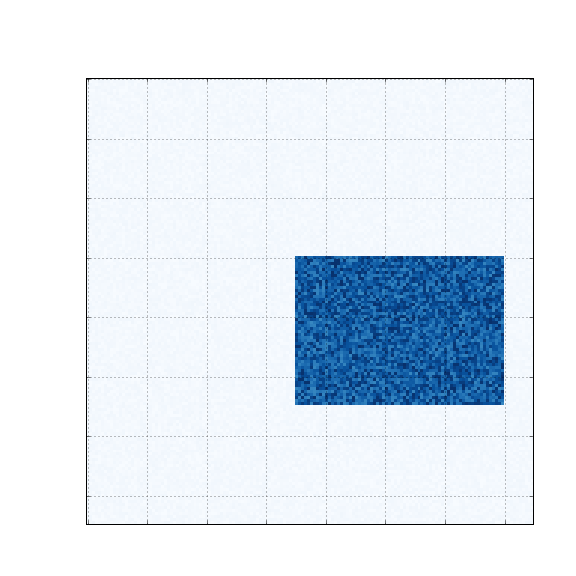
\includegraphics[width=\textwidth]{img/a-bic-structure.png}
        \caption{}
        \label{fig:bic-syntetic-structure:a}
    \end{subfigure}
    ~ %add desired spacing between images, e. g. ~, \quad, \qquad, \hfill etc.
      %(or a blank line to force the subfigure onto a new line)
    \begin{subfigure}[b]{0.18\textwidth}
        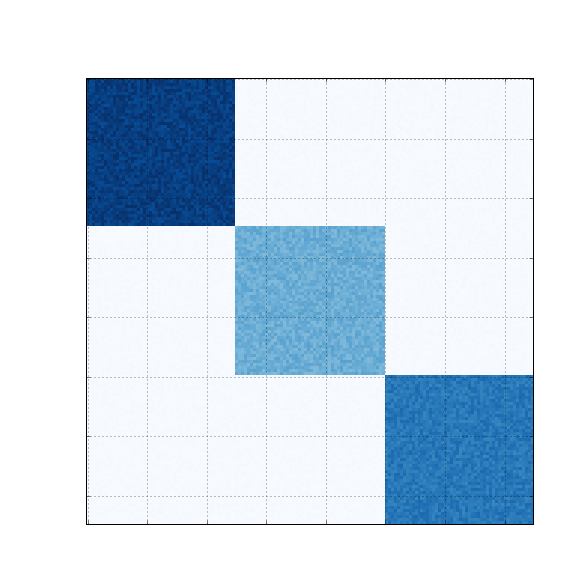
\includegraphics[width=\textwidth]{img/b-bic-structure.png}
        \caption{}
        \label{fig:bic-syntetic-structure:b}
    \end{subfigure}
    ~
    \begin{subfigure}[b]{0.18\textwidth}
        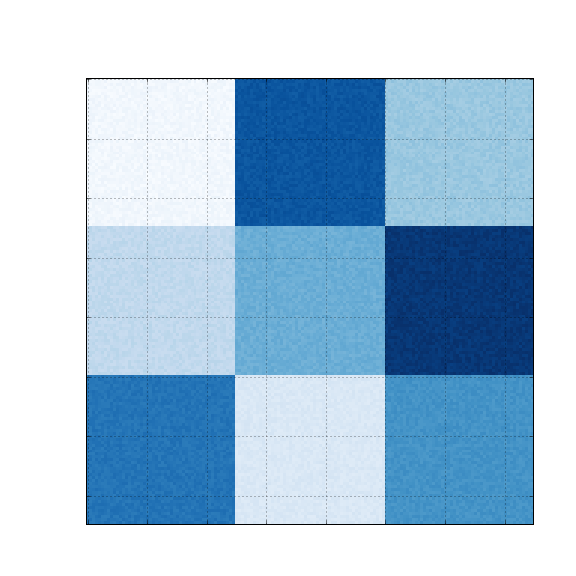
\includegraphics[width=\textwidth]{img/c-bic-structure.png}
        \caption{}
        \label{fig:bic-syntetic-structure:c}
    \end{subfigure}
    ~
    \begin{subfigure}[b]{0.18\textwidth}
        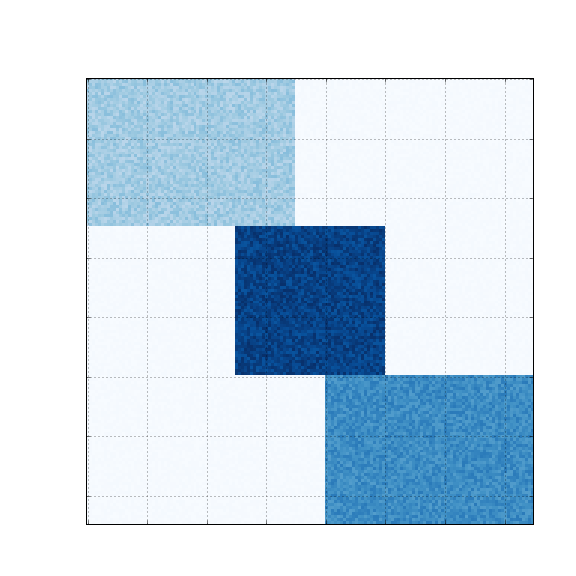
\includegraphics[width=\textwidth]{img/d-bic-structure.png}
        \caption{}
        \label{fig:bic-syntetic-structure:d}
    \end{subfigure}
    ~
    \begin{subfigure}[b]{0.18\textwidth}
        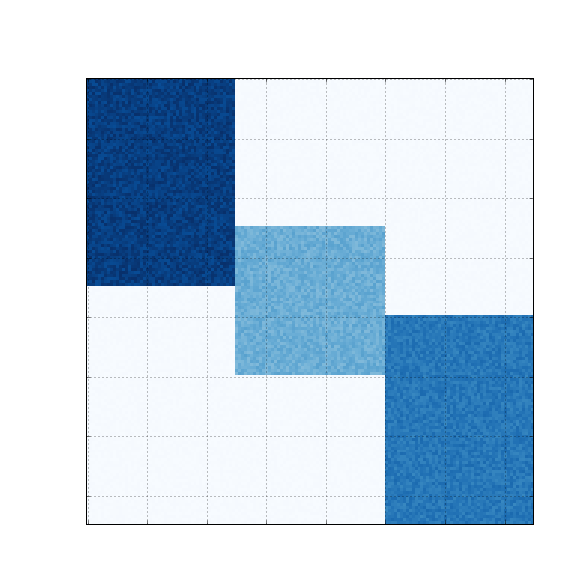
\includegraphics[width=\textwidth]{img/e-bic-structure.png}
        \caption{}
        \label{fig:bic-syntetic-structure:e}
    \end{subfigure}
    \label{fig:bic-syntetic-structure}
      \source{Lucas Fernandes Brunialti, 2016}
\end{figure}

% verificar se é cogrupo ou co-grupo
% talvez tenhamos que tratar cogrupo de interesse, pod conta da definição baseada em particionamento
Para compreender a representação gráfica apresentada na figura~\ref{fig:bic-syntetic-structure} considere que cada um dos cinco quadrados maiores representa uma base de dados sintética, que a quantidade de dados da base está representada pela altura do quadrado, que a quantidade de atributos na base está representada pela largura do quadrado. Todas as bases de dados possuem $150$ dados (linhas) e $150$ atributos (colunas). Considere ainda que cada quadrado ou retângulo, representados com diferentes tons da cor azul, representam um cogrupo, também com suas alturas e larguras representando, respectivamente, a quantidade de linhas e colunas que compõem cada cogrupo. As diferentes tonalidades da cor azul revelam a similaridade entre os valores assumidos pelos dados em subconjuntos de atributos, o que também revela a existência dos cogrupos. \textcolor{red}{A intensidade da cor é proporcional à intensidade dos valores associados a cada atributo em cada dado, então valores maiores são representados por tonalidades mais escuras e vice-versa.}

% talvez fosse interessante colocarmos um exemplo bem simples, mas numérico, no estilo que tem na tese do Fabrício.

Todas as bases de dados da figura~\ref{fig:bic-syntetic-structure} são \textcolor{red}{matrizes de valores reais positivos} geradas artificialmente. Primeiramente, uma matriz de tamanho $150 \times 150$ é preenchida com valores ponto flutuante, gerados aleatoriamente a partir de uma distribuição uniforme $unif(0,0, 1,0)$, no intervalo $[0,0, 1,0]$\footnote{Este processo evita que ocorram divisões por $0$ nos algoritmos. \textcolor{blue}{Que processo? O que exatamente evita? Ser positivo, ser uniforme? Sugiro que essa observação vá para um rodapé, mas precisa ser mais específica.}}. Em seguida, o tamanho em termo de linhas e colunas e disposição dos cogrupos na base de dados foram determinados de acordo com cada estrutura de cogrupos desejada. Para instanciar cada cogrupo, um conjunto de valores foi criado e distribuído pelas células do cogrupo da seguinte forma:

% <<<<<<< HEAD
% ************************************************************
% ************************************************************

% Podemos usar alguma coisa mais próxima de U para distribuição uniforme? Talvez Dist-U. Sei que o problema é que U é usado nos algoritmos e dist também. Mas unif ficou um pouco estranho.

% Todas as bases de dados da figura~\ref{fig:bic-syntetic-structure} são \textcolor{red}{matrizes de valores reais positivos} geradas artificialmente. Primeiramente, uma matriz de tamanho $150 \times 150$ é preenchida com valores ponto flutuante, gerados aleatoriamente a partir de uma distribuição uniforme $unif(0.0, 1.0)$, no intervalo $[0.0, 1.0]$\footnote{Este processo evita que ocorram divisões por $0$ nos algoritmos. \textcolor{red}{Que processo? O que exatamente evita? Ser positivo, ser uniforme? Sugiro que essa observação vá para um rodapé, mas precisa ser mais específica.}}. Em seguida, os cogrupos foram gerados a partir da escolha aleatória de um valor central $c \in \mathcal{C}$, sendo $\mathcal{C} = \{ 20, 40, 60, 80, 100, 120, 140, 160, 180 \}$, e da adição de valores gerados a partir da função $unif(0.0, 10.0)$ a elementos localizados a uma distância matricial \textcolor{red}{em um raio $a_1, a_2$ de $c$, respectivamente na direção das linhas e das colunas da matriz.}

% não entendi que valor C é esse, porque tem valor 160 e 180?????
% =======
% A inicialização é mesmo no intervalo de 0 a 10? Não é no intervalo de 0 a 1?
% >>>>>>> 2792448c20174b8a33ff41ecb8de077f0d58b4c5

\begin{itemize}
\item um valor central $c \in \mathcal{C}$, sendo $\mathcal{C} = \{ 20, 40, 60, 80, 100, 120, 140, 160, 180 \}$, foi aleatoriamente escolhido;
\item o conjunto de valores usado para instanciar as células do cogrupo foi estabelecido por meio da adição de $c$ a valores reais, gerados a partir da função $unif(0,0, 10,0)$, sendo que $unif$ é uma função que escolhe um valor aleatório dentro do intervalo $[0,0,10,0]$, seguindo uma distribuição uniforme;
\item  cada um dos valores nesse conjunto foi atribuído às células previamente definidas como pertecentes ao cogrupo.
\end{itemize}

%Lucas, eu resumi bastante aqui. Não considerei a variável B porque estava um pouco estranho criá-la com os indices ij e depois copiar para a matriz original assumindo os mesmos índices. Se você quiser voltar em como estava, você teria que definir melhor o procedimento de cópia (ou de inserção de B em X). Tenho o seu pdf original, então se for para voltar podemos olhar no original (se for difícil trabalhar com as versões que vc gerencia no git).

Assim, considerando que um cogrupo é uma submatriz da matriz original $X$, ele pode ser gerado pela equação % ~\ref{eq:genbic}.

\begin{equation}
\label{eq:genbic}
    x_{ij} = c + unif(0,0, 10,0)    \nonumber
\end{equation}

sendo $i$ e $j$ os índices das linhas e colunas de $X$ escolhidos para compor o cogrupo.

% Dúvida: vc faz algum controle sobre não repetir a escolha de c??? Se sim, isso precisa ficar claro aqui. E precisa também verificar a questão do 0 que você disse que evita colocar na matriz. Seu intervalor é mesmo [0,10] ou é (0,10]?

Ainda sobre a interpretação da figura~\ref{fig:bic-syntetic-structure}, alguns detalhes precisam ser observados. A depender do objetivo da análise de coagruamento, na figura~\ref{fig:bic-syntetic-structure:a}, por exemplo, mais de um cogrupo pode ser observado, \textcolor{red}{além daquele que é de interesse de análise neste trabalho}. Para essa interpretação, considera-se que todo agrupamento de linhas e de colunas, independente de serem úteis ou não, ou de serem interesse para análise ou não, é um cogrupo. Assim, tem-se os seguintes cogrupos na base de dados sintética (a):

% Conferir

\begin{itemize}
\item O mais evidente, destacado em azul, é formado pelas linhas [60 .. 109] e pelas colunas [70 .. 139]. Esse é o cogrupo de interesse, nesse projeto, para a resolução da tarefa de coagrupamento aplicada a dados textuais, e é representado na figura~\ref{fig:bic-syntetic-structure:a} pelo quadrado em cor azul.
\item O segundo, que não está destacado na visualização, é formado por todas as linhas e as colunas [0 .. 69] e [140 .. 149].
\item O terceiro, também não destacado, é formado por todas as colunas e as linhas [0 .. 59] e [110 .. 149].
\end{itemize}

Sob essa ótica de interpretação, as demais bases de dados possuem:

\begin{itemize}
\item (b): três cogrupos de principal interesse e seis cogrupos não destacados na figura;
\item (c): seis cogrupos de principal interesse;
\item (d): três cogrupos de princial interesse e oito cogrupos não destacados na figura;
\item (e): três cogrupos de princial interesse e oito cogrupos não destacados na figura.
\end{itemize}

% sugiro que seja colocada a descrição detalhada de cada um apenas se tivermos espaço, se o texto não ficar muito longo. Eventualmente, também podemos deixar em Apêndice, ou fazer uma figura também para cá ou para o Apêndice.

% ***************************************************************************
% ***************************************************************************

%Lucas, eu estou deixando o seu original mas estou propondo outra forma de descrever. Precisamos discutir qual delas vai ficar.

%\begin{itemize}
%    \item \textit{\textbf{Figura~\ref{fig:bic-syntetic-structure:a}}} há um bicluster, formado pelas linhas de $60$ à $110$ e pelas colunas de $70$ à $140$; sendo então, dois coclusters de linhas, o primeiro formado pelas linhas de $60$ à $110$ e o segundo pelas demais linhas, e dois cogrupos de colunas, o primeiro formado pelas colunas de $70$ à $140$ e o segundo pelas demais colunas.
%    \item \textit{\textbf{Figura~\ref{fig:bic-syntetic-structure:b}}} há três biclusters sem intersecção, o primeiro formado pelas linhas de $0$ à $49$ e pelas colunas de $0$ à $49$, o segundo formado pelas linhas de $50$ à $99$ e pelas colunas $50$ à $99$, o terceiro formado pelas linhas de $100$ à $149$ e pelas colunas de $100$ à $149$; sendo então, três coclusters de linhas sem intersecção e três coclusters de colunas sem intersecção, o primeiro formado pelas linhas de $0$ à $49$, o segundo formado pelas linhas de $50$ à $99$, o terceiro formado pelas linhas de $100$ à $149$, o quarto formado pelas colunas de $0$ à $49$, o quinto formado pelas colunas de $50$ à $99$, e o sexto formado pelas colunas de $100$ à $149$, respectivamente.
%   Também existe outra forma de observar os coclusters presentes neste caso, se for considerado os coclusters de colunas para cada cocluster de linhas, seriam os mesmos três coclusters de linhas e dois coclusters de colunas para cada cocluster de linha, ou seja, para o primeiro cocluster de linhas (linhas $0$ à $49$), os dois coclusters de colunas são os coclusters formados pelas colunas de $0$ à $49$ e pelas demais colunas ($50$ à $149$), seguindo a mesma lógica para os demais coclusters.
%    Note que desta maneira, é possível que coclusters de colunas tenham intersecção.
%    \item \textit{\textbf{Figura~\ref{fig:bic-syntetic-structure:c}}} há nove biclusters com intersecção em estrutura de xadrez, formados através da divisão da matriz de dados sintética em partes iguais; sendo assim, serão 3 coclusters de linhas sem intersecção e 3 coclusters de colunas sem intersecção, o primeiro formado pelas linhas de $0$ à $49$, o segundo formado pelas linhas de $50$ à $99$, o terceiro formado pelas linhas de $100$ à $149$, o quarto formado pelas colunas de $0$ à $49$, o quinto formado pelas colunas de $50$ à $99$, e o sexto formado pelas colunas de $100$ à $149$.
%    É possível fazer a mesma observação de coclusters realizada no item \textit{\textbf{Figura~\ref{fig:bic-syntetic-structure:b}}}, totalizando nove coclusters, três coclusters de linhas e três coclusters de colunas para cada cocluster de linha.
%    \item \textit{\textbf{Figura~\ref{fig:bic-syntetic-structure:d}}} há três biclusters com intersecção nas colunas, o primeiro formado pelas linhas de $0$ à $49$ e pelas colunas de $0$ à $69$, o segundo formado pelas linhas de $50$ à $99$ e pelas colunas $50$ à $99$, e o terceiro formado pelas linhas de $100$ à $149$ e pelas colunas de $79$ à $149$; sendo então, 3 coclusters de linhas sem intersecção e 3 coclusters de colunas com intersecção.
%    Considerando os coclusters de colunas para cada cocluster de linhas, serão nove coclusters, dois coclusters de colunas para cada um dos três coclusters de linhas.
%    \item \textit{\textbf{Figura~\ref{fig:bic-syntetic-structure:e}}} Este caso é exatamente igual ao item \textit{\textbf{Figura~\ref{fig:bic-syntetic-structure:d}}} se for observado a transposição da matriz de dados sintética.
% \end{itemize}

% ***************************************************************************
% ***************************************************************************

Para cada uma das bases de dados sintéticas foram executados os seguintes algoritmos: \textit{k-means}\footnote{Para os experimentos com \textit{k-means} foi usada a implementação da biblioteca \textit{scikit-learn} \cite{scikitLearn} da linguagem Python.}, \textit{fuzzy k-means}\footnote{Para experimentos com \textit{fuzzy k-means} foi usado a implementação do algoritmo \textit{fuzzy k-means} da biblioteca \textit{scikit-fuzzy} da linguagem Python.}, \textit{ONMTF}, \textit{FNMTF}, \textit{OvNMTF} e \textit{BinOvNMTF}\footnote{Os algoritmos baseadas em fatoração de matrizes foram implementados pelo autor deste trabalho usando a linguagem Python.}. Os resultados foram analisados em termos de qualidade de reconstrução, qualidade de particionamento e \textcolor{red}{qualidade de coagraumento}.
% não tem uma referência para a biblioteca fo fuzzy k-means??????

\subsection{Análise da reconstrução}

% para isso valer vamos ter que definir kmeans e fuzzy k means em termos de fatoração de matrizes; ou mudar um pouco essa frase aqui.
% porém, pela forma como foi explicado mais abaixo, acho que vamos ter que melhorar aqui já explicando aqui o que é a resconstruação para o kmeans e o fuzzy k means.
% Uma forma de analisar o resultado dos algoritmos estudados neste trabalho é analisá-los quanto a sua capacidade de reconstrução. Para os algoritmos baseados em fatoração de matrizes, a reconstrucão é feita tomando as matrizes resultantes da fatoração e combinando-as \textcolor{red}{da mesma forma que o seu problema foi proposto}, de forma a reconstruir a matriz original. \textcolor{red}{Para o caso dos algoritmos \textit{k-means} e \textit{fuzzy-k-means}, a resconstrução foi representada pela substituição do valor do centróide ....}
% % eu não entendi o que foi feito não. Ver com Lucas, e no caso do fuzzy k means ver como foi o tratamento da pertinência.

% Essa análise se torna importante a partir do momento em que se tem como objetivo avaliar o comportamento dos algoritmos em diferentes estruturas de organização de cogrupos. A capacidade de reconstrução .... \textcolor{red}{vamos ver se colocamos alguma coisa a mais para justificar esse análise.}
Uma forma de analisar o resultado dos algoritmos estudados neste trabalho é analisá-los quanto a sua capacidade de reconstrução. Para os algoritmos baseados em fatoração de matrizes, a reconstrucão é feita tomando as matrizes resultantes da fatoração e combinando-as \textcolor{red}{da mesma forma que o seu problema foi proposto}, de forma a reconstruir a matriz original. Para o caso dos algoritmos \textit{k-means} e \textit{fuzzy-k-means}, a resconstrução foi realizada assumindo que os centróides obtidos pelos algoritmos representam os dados originais; assim a substituição de um dado original pelo centróide do grupo ao qual ele pertence, seguindo as regras dos algoritmos \textit{k-means} e \textit{fuzzy k-means}, constitui a reconstrução aplicada nesses casos.
% ainda acho que alguma consideração a mais deveria ser feita no fuzzy k-means.
% e uma outra coisa importante: se os demais algoritmos também nos dão centróides, então a mesma coisa feita com kmeans e fuzzy-k-means não deveria ser feita com eles???????

Essa análise se torna importante quando se tem como objetivo avaliar o comportamento dos algoritmos em diferentes estruturas de organização de cogrupos, com destaque para a análise de maior interesse neste trabalho -- \textcolor{red}{coagrupamento com interseção de linhas ou colunas.} \textcolor{blue}{A capacidade de reconstrução .... vamos ver se colocamos alguma coisa a mais para justificar esse análise.}
% TODO Descrever melhor pq a reconstrução é importante

Um resumo sobre os resultados obtidos nessa análise é apresentado na tabela~\ref{tab:resumoREC}. O restante dessa seção se destina a detalhar as análise de qualidade de reconstrução.

\begin{table}[htpb]
\centering
    \caption{Resumo de qualidade de reconstrução: ok - permite reconstrução; * - sem informação sobre interseção; + - preserva informação de interseção}
        \begin{tabular}{cccccc}
            \hline
            & \textbf{base (a)} & \textbf{base (b)} & \textbf{base (c)} & \textbf{base (d) }& \textbf{base (e)} \\
            \hline
            \textit{k-means}       & ok & ok & ok & ok*  &  \\
            \textit{  fuzzy-k-means} & ok & ok & ok & ok*  &  \\
            ONMTF         & ok & ok & ok & +    & +  \\
            FNMTF         & ok & ok & ok &    &  \\
            OvNMTF        & ok & ok & ok & ok+  & + \\
            BinOvNMTF     & ok & ok & ok & ok+  &  \\
            \hline
             & & & & &  \\
        \end{tabular}
%    }
    \label{tab:resumoREC}
    \source{Lucas Fernandes Brunialti, 2016}
\end{table}


% uma dúvida. O que estamos fazendo é multiplicando a matriz de pertinências (que aqui assume 0 e 1 pelos centróides, correto? Esse não é o mesmo procedimento feito para os algoritmos de fatoração de matrizes? E se é, no caso do fuzzy-c-means, temos a matriz de pertinência não binária. Não deveríamos simplementes multiplicá-la pelos centróides?

\subsection{Reconstrução a partir dos resultados do algoritmo \textit{k-means}}
\label{subsec:results-reconstruction-kmeans}

% Lucas, verifique o erro mínimo buscado por favor, está estranho.
Para execução dos experimentos com o \textit{k-means} os seguintes parâmetros foram estabelecidos: número máximo de iterações ($300$) ou  \textcolor{red}{a diferença do erro de minimização em duas iterações consecutivas ($\leq 1,0 * 10^{-4}$)}, o que ocorrer primeiro, como critérios de parada; número de grupos $k = 2$ para a base de dados sintética (a) e $k = 3$ para as bases de dados sintéticas (b), (c), (d) e (e). \textcolor{red}{A escolha de $k$ foi realizada com a prerrogativa de que o algoritmo \textit{k-means} deveria encontrar os grupos considerando todos os atributos descritivos, e desta forma, agrupar os dados de acordo com a similaridade total. Assim, $k$ foi escolhido a partir da quantidade de agrupamento de linhas presente na base de dados. A escolha de $k$ maiores levaria o algoritmo a, necessariamente, dividir em grupos diferentes os dados que deveriam pertencer a um mesmo agrupamento de linhas.} Foram executadas $10$ rodadas do algoritmo, com \textcolor{red}{inicialização de centróides aleatória}, sendo que o melhor modelo resultante nessas rodadas foi escolhido para ilustrar a avaliação da qualidade da reconstrução.
% verificar com Lucas pois acho que ele usou o k-means ++

As reconstruções obtidas a partir dos centróides encontrados pelo algoritmo \textit{k-means} são ilustradas Figura~\ref{fig:reconstruction:kmeans}. As matrizes originais são repetidas na figura, nas cinco primeiras posições, de forma a facilitar a análise visual dos resultados. Para um melhor entendimento da representação gráfica, note que cada linha recebe cores de acordo com sua pertinência a um agrupamento de linhas (ou grupo, na visão de agrupamento) representado por um centróide. Ou seja, se a linha $10$ pertencer ao centróide $1$, então os valores da linha $10$ serão substituídos pelos valores do centróide $1$. Note que o centróide é um vetor com o mesmo número de coordenadas de um dado da base de dados, sendo assim, a substituição é direta. O centróide que representa o agrupamento de linhas referente ao cogrupo de interesse (em azul na figura), possui, claramente, valores similares aos dados que pertencem a esse cogrupo, e por isso o procedimento proposto pode ser visto como uma representação de reconstrução.

\begin{figure}[H]
    \caption{
        As primeiras cinco matrizes são as matrizes originais, as demais são suas respectivas reconstruções, realizadas a partir dos resultados obtidos com o algoritmo \textit{k-means}.
    }
\centering
    \begin{subfigure}[b]{0.18\textwidth}
        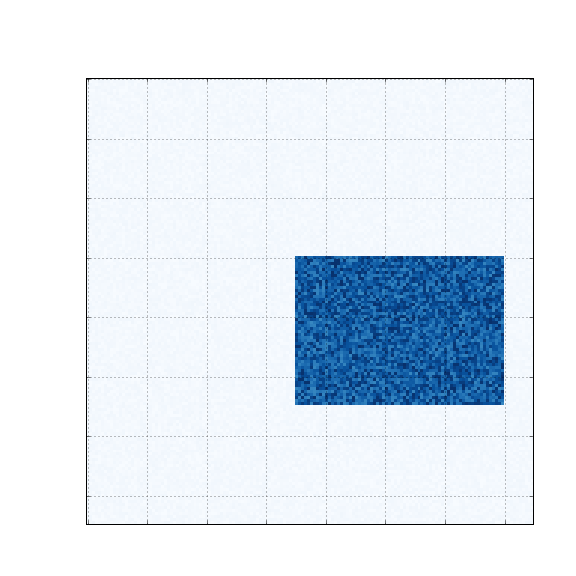
\includegraphics[width=\textwidth]{img/a-bic-structure.png}
    \end{subfigure}
    \begin{subfigure}[b]{0.18\textwidth}
        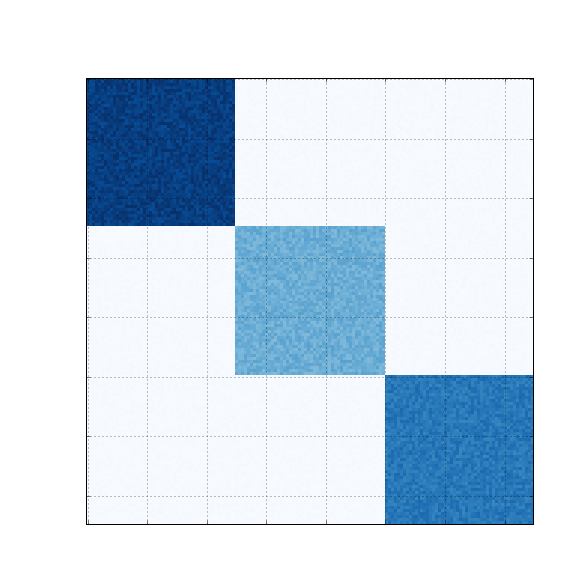
\includegraphics[width=\textwidth]{img/b-bic-structure.png}
    \end{subfigure}
    \begin{subfigure}[b]{0.18\textwidth}
        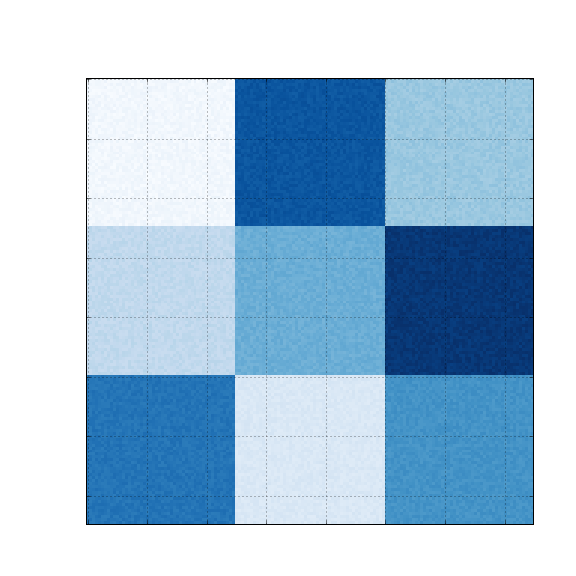
\includegraphics[width=\textwidth]{img/c-bic-structure.png}
    \end{subfigure}
    \begin{subfigure}[b]{0.18\textwidth}
        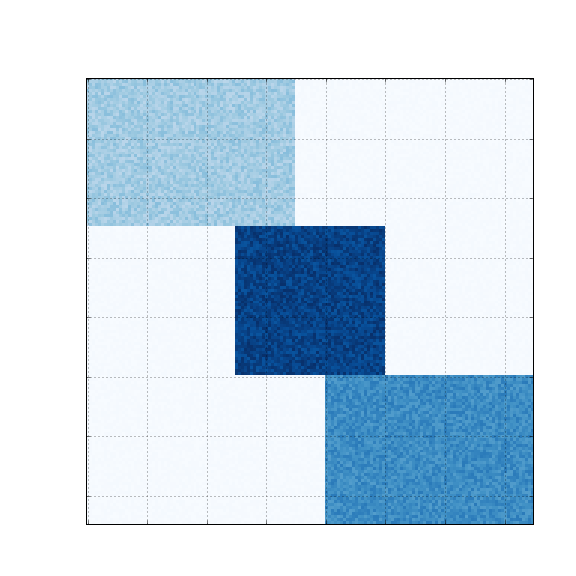
\includegraphics[width=\textwidth]{img/d-bic-structure.png}
    \end{subfigure}
    \begin{subfigure}[b]{0.18\textwidth}
        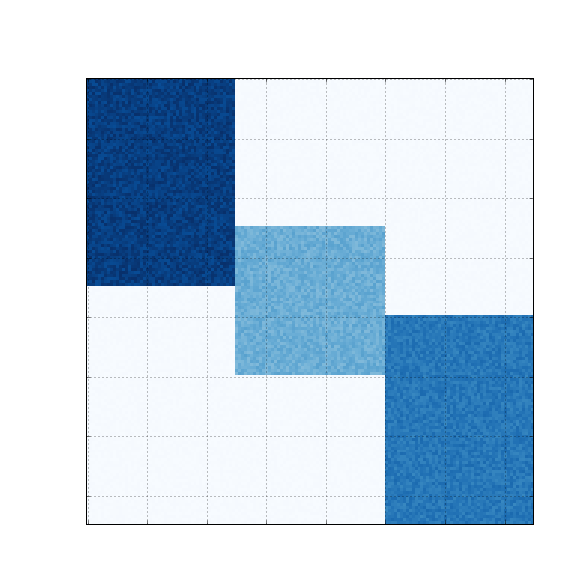
\includegraphics[width=\textwidth]{img/e-bic-structure.png}
    \end{subfigure}

    \begin{subfigure}[b]{0.18\textwidth}
        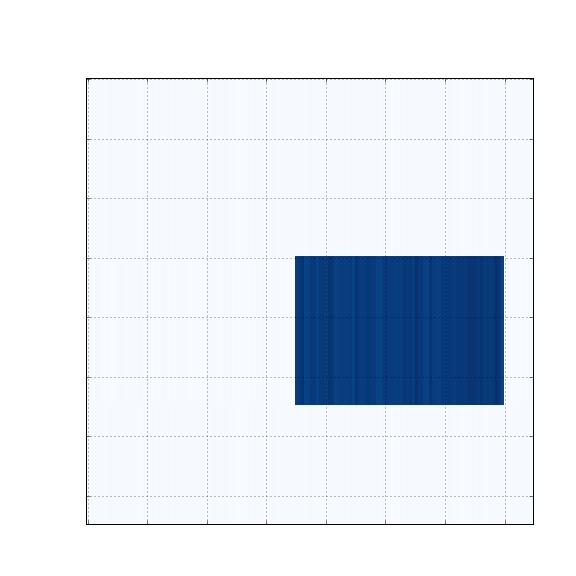
\includegraphics[width=\textwidth]{img/a-reconstruction-kmeans.png}
        \caption{}
    \end{subfigure}
    \begin{subfigure}[b]{0.18\textwidth}
        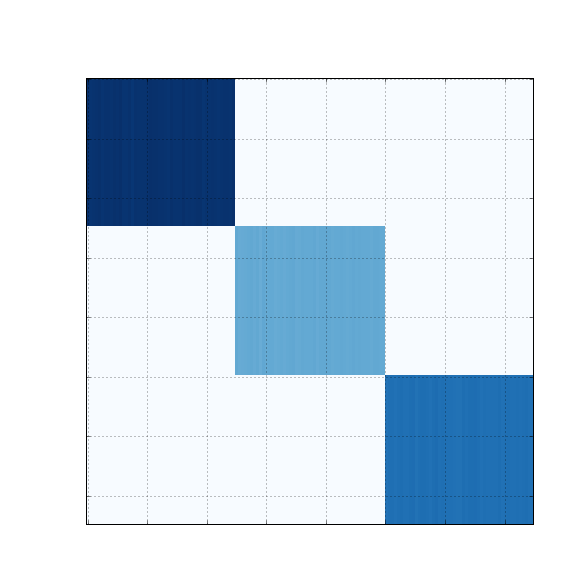
\includegraphics[width=\textwidth]{img/b-reconstruction-kmeans.png}
        \caption{}
    \end{subfigure}
    \begin{subfigure}[b]{0.18\textwidth}
        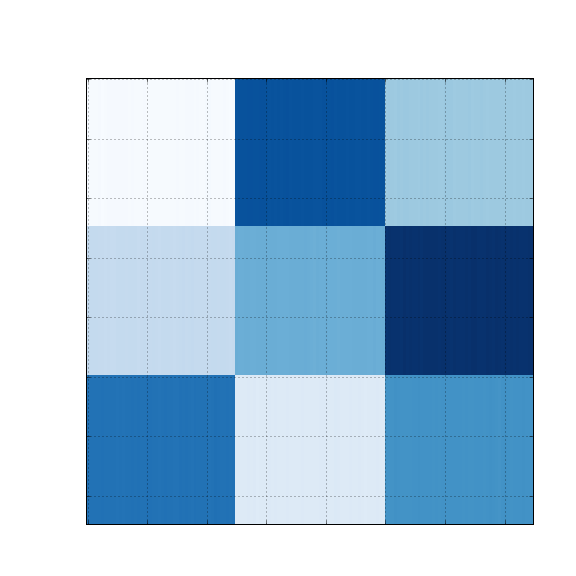
\includegraphics[width=\textwidth]{img/c-reconstruction-kmeans.png}
        \caption{}
    \end{subfigure}
    \begin{subfigure}[b]{0.18\textwidth}
        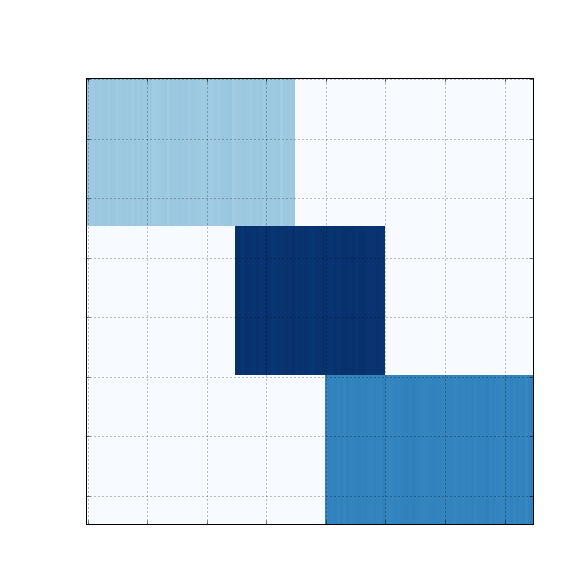
\includegraphics[width=\textwidth]{img/d-reconstruction-kmeans.png}
        \caption{}
    \end{subfigure}
    \begin{subfigure}[b]{0.18\textwidth}
        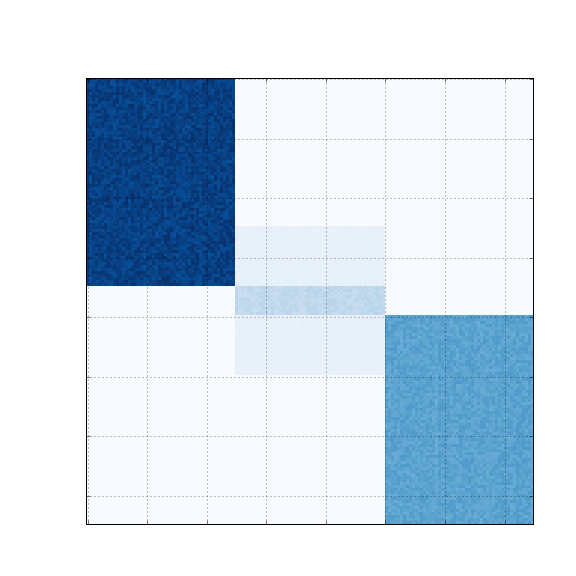
\includegraphics[width=\textwidth]{img/e-reconstruction-kmeans.png}
        \caption{}
    \end{subfigure}
    \label{fig:reconstruction:kmeans}
          \source{Lucas Fernandes Brunialti, 2016}
\end{figure}

% as cores não correspondem na reconstrução. Me lembro de isso ser devido a alguma normalização. Então precisa esclarecer aqui. Acho que uma nota de rodapé resolve.

O modelo resultante da execução do \textit{k-means} \textcolor{red}{permite representar perfeitamente a  reconstrução} para as bases de dados (a) à (d). Porém, é preciso lembrar que não há informação sobre agrupamento de colunas no resultado do algoritmo, sendo que a visualização gráfica de cada coagrupamento é possível apenas por conta da similaridade do centróide em relação aos dados de cada agrupamento de linhas.

O modelo não permite a descoberta de grupos com interseção de linhas (um dado não pode pertencer a mais de um grupo), e portanto não permite uma boa representação para a reconstrução no caso da base de dados (e). Esse resultado já era esperado devido à natureza da solução apresentada pelo \textit{k-means}. \textcolor{blue}{Tem um erro aqui, pois o centróide deveria ser único para cada um dos 3 grupos, não há como termos esse quarto quadrado em azul claro.}


\subsection{Reconstrução a partir dos resultados do algoritmo \textit{fuzzy k-means}}
\label{subsec:results-reconstruction-fkmeans}

% verificar se podemos chamar de parâmetro de fuzzyficação
% Há uma justificativa para m=2, vamos colocar aqui.
% TODO eu li que esse é o usual (default), explicar pq
Os mesmos critérios de parada e número de grupos usados para o \textit{k-means} foram também usados nos experimentos com o \textit{fuzzy k-means}. O valor para o parâmetro de fuzzificação $m$ foi mantido em $2$, como indicado em \cite{Peres2012}. Também, $10$ execuções foram realizadas, com iniciação aleatória de pesos e o melhor modelo obtido foi usado para avaliação da qualidade de reconstrução obtida.

% O parâmetro de fuzzyficação m é geralmente valorado com 2 para permitir que a pertinência de dados a grupos sejam obtidas unicamente em função das razões entre as distâncias entre dados e centros de grupos. Valores maiores do que 2 fazem com que as pertinências obtidas sejam influenciadas pela quantidade de grupos; valores menores do que 2 (se aproximando de 1, limite inferior para este parâmetro) aproxima o resultado do fuzzy-k-means do k-means pois as diferenças entre as pertinências tendem a aumentar.

Da mesma forma que o experimento anterior, as reconstruções apresentadas na figura~\ref{fig:reconstruction:fkmeans} foram obtidas por meio da coloração de linhas de acordo com os centróides resultantes da execução do algoritmo, e as matrizes originais foram repetidas para facilitar a análise visual. Contudo, desde que a pertinência de um dado a mais de um grupo é possível nesse algoritmo, escolheu-se o grupo ao qual o dado tem maior pertinência para usar como base para a reconstrução.

\begin{figure}[H]
\centering
    \caption{
        As primeiras cinco matrizes são as matrizes originais, as demais são suas respectivas reconstruções, realizadas a partir dos resultados obtidos com o algorimto \textit{fuzzy k-means}.
    }
    \begin{subfigure}[b]{0.18\textwidth}
        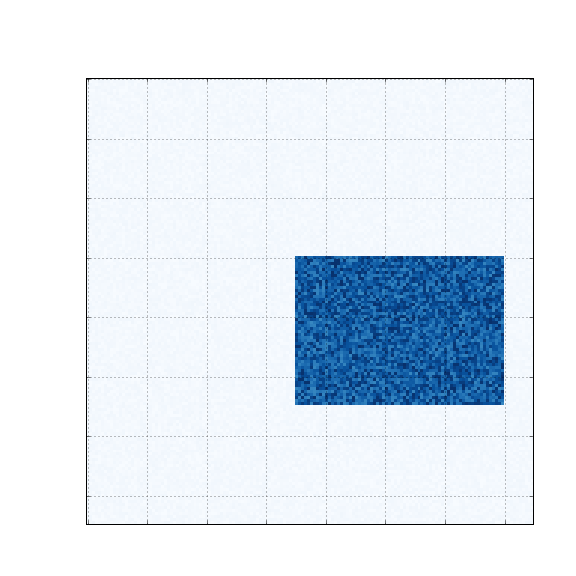
\includegraphics[width=\textwidth]{img/a-bic-structure.png}
    \end{subfigure}
    \begin{subfigure}[b]{0.18\textwidth}
        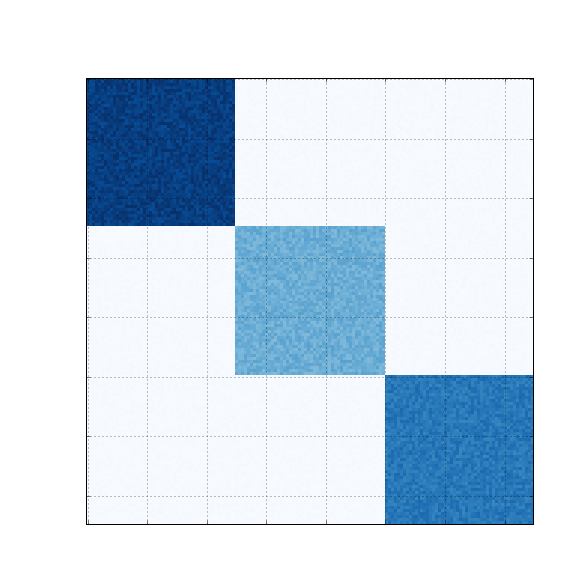
\includegraphics[width=\textwidth]{img/b-bic-structure.png}
    \end{subfigure}
    \begin{subfigure}[b]{0.18\textwidth}
        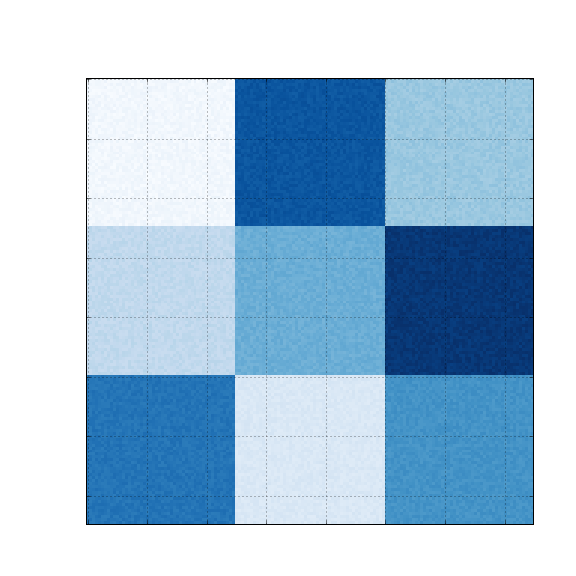
\includegraphics[width=\textwidth]{img/c-bic-structure.png}
    \end{subfigure}
    \begin{subfigure}[b]{0.18\textwidth}
        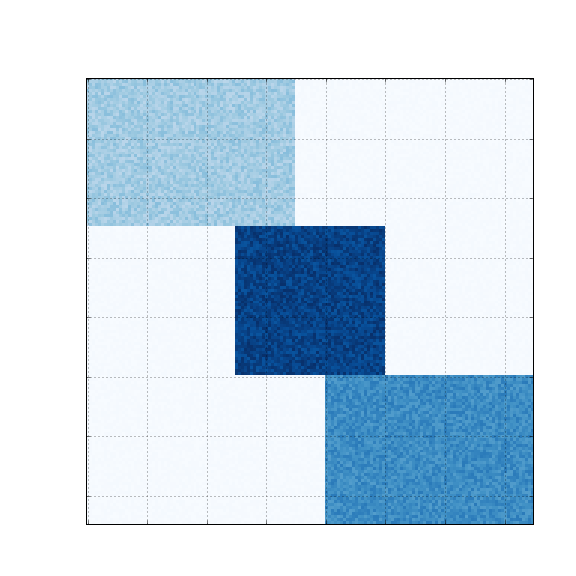
\includegraphics[width=\textwidth]{img/d-bic-structure.png}
    \end{subfigure}
    \begin{subfigure}[b]{0.18\textwidth}
        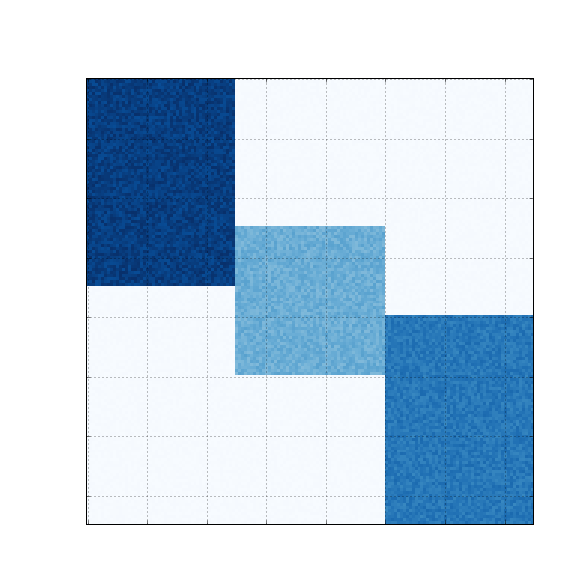
\includegraphics[width=\textwidth]{img/e-bic-structure.png}
    \end{subfigure}

    \begin{subfigure}[b]{0.18\textwidth}
        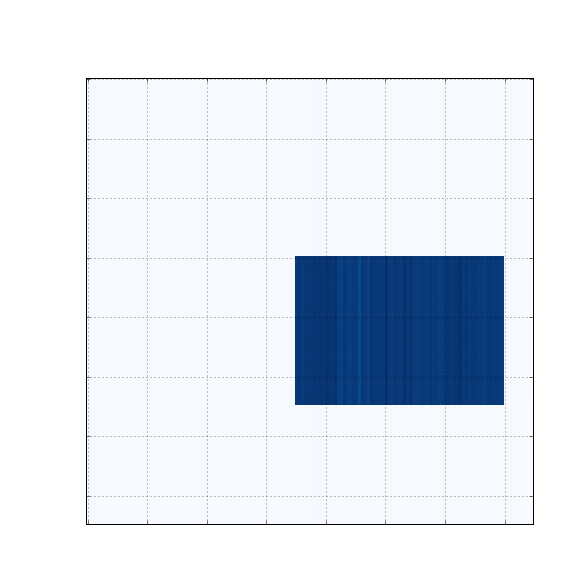
\includegraphics[width=\textwidth]{img/a-reconstruction-fkmeans.png}
        \caption{}
    \end{subfigure}
    \begin{subfigure}[b]{0.18\textwidth}
        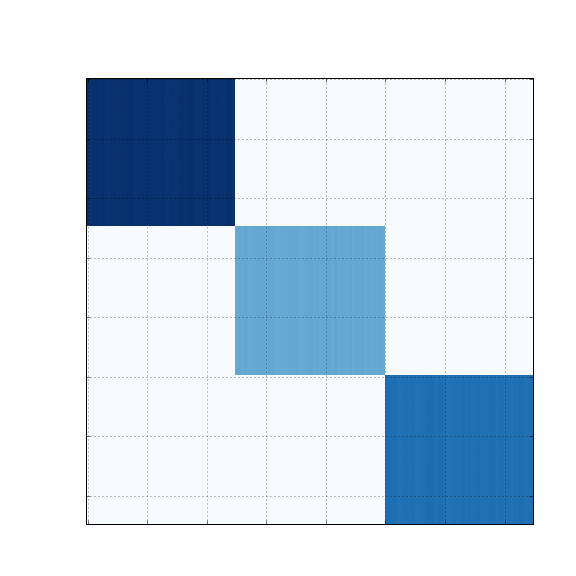
\includegraphics[width=\textwidth]{img/b-reconstruction-fkmeans.png}
        \caption{}
    \end{subfigure}
    \begin{subfigure}[b]{0.18\textwidth}
        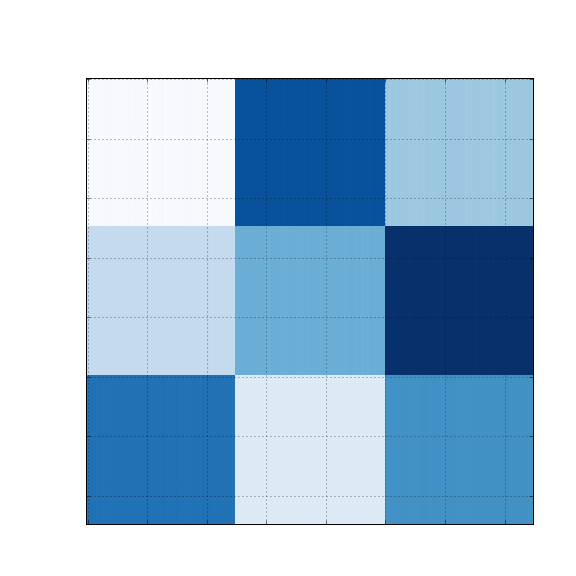
\includegraphics[width=\textwidth]{img/c-reconstruction-fkmeans.png}
        \caption{}
    \end{subfigure}
    \begin{subfigure}[b]{0.18\textwidth}
        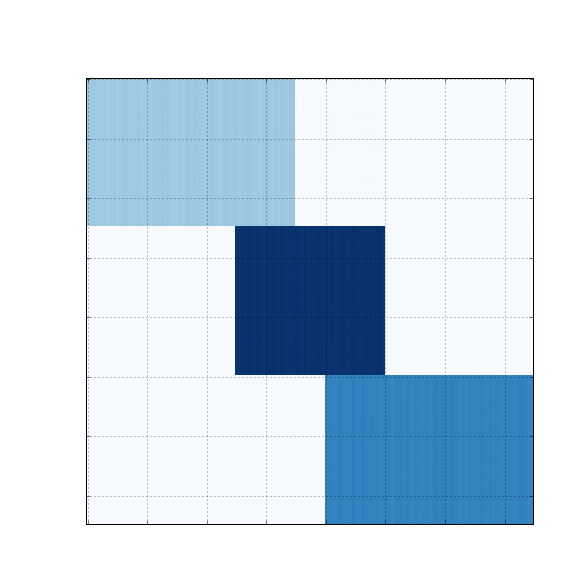
\includegraphics[width=\textwidth]{img/d-reconstruction-fkmeans.png}
        \caption{}
    \end{subfigure}
    \begin{subfigure}[b]{0.18\textwidth}
        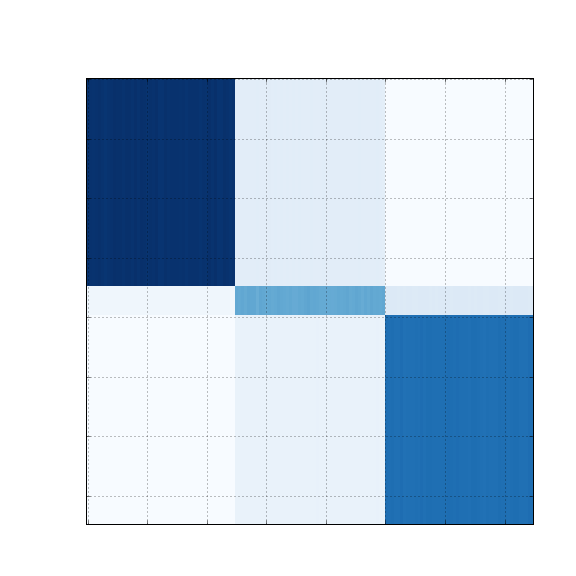
\includegraphics[width=\textwidth]{img/e-reconstruction-fkmeans.png}
        \caption{}
    \end{subfigure}
    \label{fig:reconstruction:fkmeans}
        \label{fig:reconstruction:kmeans}
\source{Lucas Fernandes Brunialti, 2016}
\end{figure}

% porém, apesar do algoritmo lidar com intersecção de clusters, este não foi capaz de fazer a reconstrução do caso (e).
% TODO dizer que no (e) foi pior que o kmeans?
% no kmeans parece que há uma variação dentro dos cogrupos que aqui não há. Seria interessante falar sobre isso?

% o caso E aqui está fazendo mais sentido que no kmeans e considerando a maior pertinência, deveria ser parecido no kmenas. Ou aqui seria melhor por indicar que há uma influencia diferentes naqueles atributos que tem algum coloracao, o que não kmeans não ocorre. Mas deveria ocorrer pois o centróide é media na coluna.

De forma semelhante à análise de reconstrução proporcionada pelo \textit{k-means}, o \textit{fuzzy k-means} também \textcolor{red}{permite representar perfeitamente a reconstrução} para as bases de dados (a) à (d). Porém, a reconstrução para o caso (e) não foi obtida com sucesso. Embora o \textit{fuzzy c-means} lide, em sua concepção, com sobreposição de grupos, neste caso representada pelas pertinências fuzzy dos dados a vários grupos, o procedimento de escolha da maior pertinência anula essa capacidade na representação da reconstrução; \textcolor{blue}{muito embora .... é preciso fazer alguma ressalva ou análise diferente aqui.}

% aqui tem fuzzificação, verificar com Lucas. E se for feita com a segunda maior pertinência? Haverá alguma informação que complete a reconstrucão feita com a primeira???? Seria legal pensar nisso.

% eu acho que tem que ter um paralelo diferente aqui, pois a matriz de pertinências nesse caso é parecida com a matriz S dos algoritmos de fatoração.
>>>>>>> 2792448c20174b8a33ff41ecb8de077f0d58b4c5

\subsection{Reconstrução a partir dos resultados do algoritmo \textit{ONMTF}}
\label{subsec:results-reconstruction-onmtf}

%originalmente Lucas informou que k = l = 3 para os cadaos c d e e. É isso mesmo? Eu troquei.

Para execução dos experimentos com o ONMTF a seguinte parametrização foi estabelecida: número máximo de iterações ($1000$) ou \textcolor{red}{a diferença do erro de minimização em duas iterações consecutivas ($\leq 1,0 * 10^{-4})$}, o que ocorrer primeiro, como critérios de parada; o número de cogrupos de linhas ($k$) e colunas ($l$) configurados da seguinte maneira: \textcolor{red}{$k = l = 2$ para (a), $k = 3$ e $l = 2$ para (b), (d) e (e), e $k = l = 3$ para (c)}. Novamente, as escolhas são baseadas no conhecimento \textit{apriori} que se tem sobre a quantidade de cogrupos, e quais cogrupos, deseja-se obter. Para a execução do algoritmo \textit{ONMTF} é necessária a normalização dos dados, então, todas as matrizes de dados sintéticas foram normalizadas para que a norma das linhas fosse igual à $1$.
% náo precisaríamos indicar a operação aqui?

A partir da realização de $10$ execuções do algoritmo, foi escolhido o modelo que alcançou a menor taxa de erro e a partir do resultado obtido a reconstrução foi avaliada. A qualidade das resconstruções pode ser visualmente observada na figura~\ref{fig:reconstruction:onmtf}. A resconstrução foi obtida a partir da multiplicação das matrizes fatoradas, ou seja, \textcolor{red}{$USV^T$}, conforme explicado no capítulo~\ref{ch:fatoracao}.
\begin{figure}[H]
\centering
    \caption{
        As primeiras cinco matrizes são as matrizes originais, as demais são suas respectivas reconstruções, realizadas a partir dos resultados obtidos com o algoritmo \textit{ONMTF}.
    }
    \begin{subfigure}[b]{0.18\textwidth}
        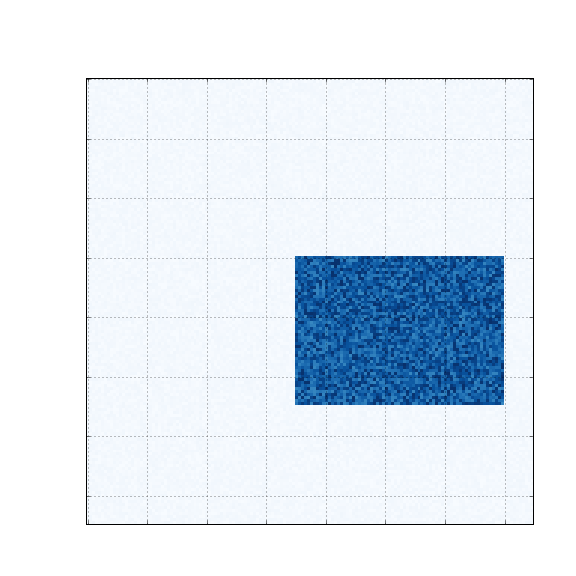
\includegraphics[width=\textwidth]{img/a-bic-structure.png}
    \end{subfigure}
    \begin{subfigure}[b]{0.18\textwidth}
        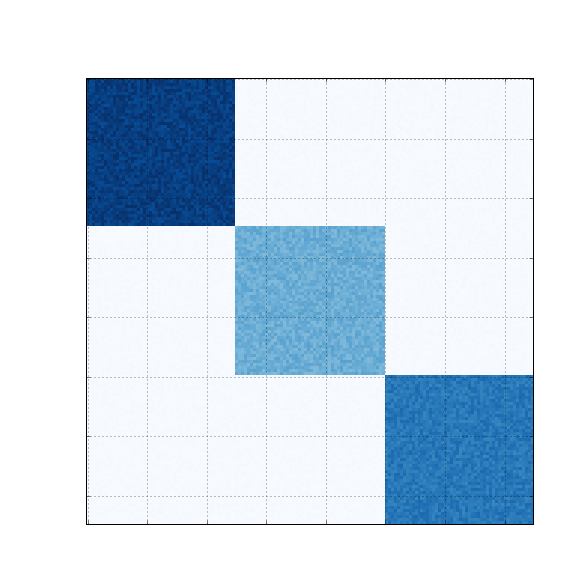
\includegraphics[width=\textwidth]{img/b-bic-structure.png}
    \end{subfigure}
    \begin{subfigure}[b]{0.18\textwidth}
        \includegraphics[width=\textwidth]{img/c-bic-structure.png}
    \end{subfigure}
    \begin{subfigure}[b]{0.18\textwidth}
        \includegraphics[width=\textwidth]{img/d-bic-structure.png}
    \end{subfigure}
    \begin{subfigure}[b]{0.18\textwidth}
        \includegraphics[width=\textwidth]{img/e-bic-structure.png}
    \end{subfigure}

    \begin{subfigure}[b]{0.18\textwidth}
        \includegraphics[width=\textwidth]{img/a-reconstruction-onmtf.png}
        \caption{}
    \end{subfigure}
    \begin{subfigure}[b]{0.18\textwidth}
        \includegraphics[width=\textwidth]{img/b-reconstruction-onmtf.png}
        \caption{}
    \end{subfigure}
    \begin{subfigure}[b]{0.18\textwidth}
        \includegraphics[width=\textwidth]{img/c-reconstruction-onmtf.png}
        \caption{}
    \end{subfigure}
    \begin{subfigure}[b]{0.18\textwidth}
        \includegraphics[width=\textwidth]{img/d-reconstruction-onmtf.png}
        \caption{}
    \end{subfigure}
    \begin{subfigure}[b]{0.18\textwidth}
        \includegraphics[width=\textwidth]{img/e-reconstruction-onmtf.png}
            \caption{}
    \end{subfigure}
\label{fig:reconstruction:onmtf}
\source{Lucas Fernandes Brunialti, 2016}
\end{figure}

% Aqui até as cores são identicas nos três primeiros casos. Não deveríamos ressaltar isso?

Analisando os resultados, é possível perceber que a reconstrução é realizada com êxito nos casos (a), (b) e (c). \textcolor{red}{O algoritmo falhou em reconstruir a matriz no caso (d) pois não foi capaz de associar corretamente as colunas que pertencem a mais de um agrupamento de colunas (interseção nas colunas). O mesmo efeito ocorre com o caso (e), no qual há interseção de linhas. A falha da reconstrução é percebida na coloração diferenciada, formando regiões com sombras, nas colunas, ou linhas, envolvidas nas interseções.}
% estava o contrário, ver com Lucas

A coloração diferenciada daquela esperada (seguindo a matriz original) é resultante do estado da matriz $V$, que contém as relações de associação de linhas e/ou colunas aos cogrupos. Para o caso (d), por exemplo, é possível deduzir, a partir da análise visual, que há valores de magnitude diferentes estabelecendo a associação das colunas \textcolor{blue}{X x X, Y x Y e Z x Z, ao grupo de linhas X x X}. Isso é possível pois o algoritmo não força a associação única e exclusiva entre uma linha e um agrupamento de linhas ou uma coluna e um agrupamento de colunas.Em uma análise qualitativa, poder-se-ia então dizer que o algoritmo está indicando a formação de quatro grupos de colunas em relação ao mesmo grupo de linhas \textcolor{blue}{X x X}.

% reescrito acima.
% No entanto, é possível ver sombras nas regiões das matrizes reconstruídas com intersecção de biclusters, isso significa que quando observa-se a matriz $V$ (que contém as relações de pertinência entre coclusters e colunas (características)) para o caso (d), é possível ver valores associados ao segundo cocluster, porém menores que as outras associações com os clusters. Isso é possível pois o algoritmo não força a associação única e exclusiva entre uma linha e um cocluster ou uma coluna e um cocluster.

\subsection{Reconstrução a partir dos resulatdos do algoritmo \textit{FNMTF}}
\label{subsec:results-reconstruction-fnmtf}

%originalmente Lucas informou que k = l = 3 para os cadaos c d e e. É isso mesmo? Eu troquei.

Para execução dos experimentos com o FNMTF a seguinte parametrização foi estabelecida: número máximo de iterações ($300$) ou \textcolor{red}{a diferença do erro de minimização em duas iterações consecutivas ($\leq 1,0 * 10^{-4}$)}, o que ocorrer primeiro, como critérios de parada; o número de cogrupos de linhas ($k$) e colunas ($l$) configurados da seguinte maneira: \textcolor{red}{$k = l = 2$ para (a), $k = 3$ e $l = 2 $ para (b), (d) e (d), e $k = l = 3$ para (c)}. Para a execução do algoritmo ONMTF é necessária a normalização dos dados, então, todas as matrizes de dados sintéticas foram normalizadas para que a norma das linhas fosse igual à $1$.

A partir da realização de $10$ execuções do algoritmo, foi escolhido o modelo que alcançou a menor taxa de erro e a partir do resultado obtido a reconstrução foi avaliada. A qualidade das reconstruções pode ser visualmente observada na figura~\ref{fig:reconstruction:fnmtf}. A reconstrução foi obtida a partir da multiplicação das matrizes fatoradas, ou seja, $FSG^T$, conforme explicado no capítulo~\ref{ch:fatoracao}.

\begin{figure}[H]
\centering
    \caption{
        As primeiras cinco matrizes são as matrizes originais, as demais são suas respectivas reconstruções, realizadas a partir dos resultados obtidos com o algoritmo \textit{FNMTF}.
    }
    \begin{subfigure}[b]{0.18\textwidth}
        \includegraphics[width=\textwidth]{img/a-bic-structure.png}
    \end{subfigure}
    \begin{subfigure}[b]{0.18\textwidth}
        \includegraphics[width=\textwidth]{img/b-bic-structure.png}
    \end{subfigure}
    \begin{subfigure}[b]{0.18\textwidth}
        \includegraphics[width=\textwidth]{img/c-bic-structure.png}
    \end{subfigure}
    \begin{subfigure}[b]{0.18\textwidth}
        \includegraphics[width=\textwidth]{img/d-bic-structure.png}
    \end{subfigure}
    \begin{subfigure}[b]{0.18\textwidth}
        \includegraphics[width=\textwidth]{img/e-bic-structure.png}
    \end{subfigure}

    \begin{subfigure}[b]{0.18\textwidth}
        \includegraphics[width=\textwidth]{img/a-reconstruction-fnmtf.png}
        \caption{}
    \end{subfigure}
    \begin{subfigure}[b]{0.18\textwidth}
        \includegraphics[width=\textwidth]{img/b-reconstruction-fnmtf.png}
        \caption{}
    \end{subfigure}
    \begin{subfigure}[b]{0.18\textwidth}
        \includegraphics[width=\textwidth]{img/c-reconstruction-fnmtf.png}
        \caption{}
    \end{subfigure}
    \begin{subfigure}[b]{0.18\textwidth}
        \includegraphics[width=\textwidth]{img/d-reconstruction-fnmtf.png}
        \caption{}
    \end{subfigure}
    \begin{subfigure}[b]{0.18\textwidth}
        \includegraphics[width=\textwidth]{img/e-reconstruction-fnmtf.png}
    \caption{}
    \end{subfigure}
    \label{fig:reconstruction:fnmtf}
\source{Lucas Fernandes Brunialti, 2016}
\end{figure}

Este caso é semelhante ao anterior (algoritmo \textit{ONMTF}). O algoritmo permitiu a reconstrução com êxito dos casos (a), (b) e (c), falhando na reconstrução dos casos (d) e (e), nos quais há intersecção de colunas ou linhas nos cogrupos de interesse. No entanto, nesse caso o algoritmo restringe a associação de linhas (ou colunas), a apenas um agrupamento de linhas (ou de colunas), e por isso a informação referente a intersecção em cogrupos é totalmente descaracterizada. Observe, por exemplo, que a reconstrução no caso (d) se assemelha à reconstrução do caso (c), embora as matrizes originais, em cada caso, representem informação sobre associação de dados e atributos em cogrupos também diferenciada.

\subsection{Reconstrução a partir dos resultados do algoritmo \textit{OvNMTF}}
\label{subsec:results-reconstruction-ovnmtf}

% e nessa caso, lucas informou que k = 3 e l = 2 para c d e d, mas no c precisava ser tudo igual a 3, correto?

Para execução dos experimentos com o \textit{OvNMTF} a seguinte parametrização foi estabelecida: número máximo de iterações ($1000$) ou \textcolor{red}{a diferença do erro de minimização ($\leq 1,0*10^{-4}$)}, o que ocorrer primeiro, como critérios de parada; o número de cogrupos de linhas ($k$) e colunas ($l$) configurados da seguinte maneira: \textcolor{red}{$k = l = 2$ para (a), $k = 3$ e $l = 2 $ para (b), (d) e (d), e $k = l = 3$ para (c)}. Para a execução do algoritmo \textit{OvNMTF} é necessária a normalização dos dados, então, todas as matrizes de dados sintéticas foram normalizadas para que a norma das linhas fosse igual à $1$.

% náo precisaríamos indicar a operação aqui?

% Como critério de parada do algoritmo, foi utilizada $1000$ como número máximo de iterações, ou a diferença do erro de minimização assumir valor menor ou igual à $1e-4$. Os parâmetros do número de coclusters de linhas e colunas foi configurado da seguinte maneira: $k = l = 2$ para (a); e $k = 3$ e $l = 2$ para (b), (c), (d) e (e). Para o funcionamento do algoritmo \textit{OvNMTF} é necessária a normalização dos dados, então, todas as matrizes de dados sintéticas foram normalizadas para que a norma das linhas seja igual à $1$.

% isso está repetindo muito, e a normalização e parametrizácão também, eu acho que é melhor colocar tudo no começo, ou em uma tabela. Acertar isso depois.
A partir da realização de $10$ execuções do algoritmo, foi escolhido o modelo que alcançou a menor taxa de erro e a partir do resultado obtido a reconstrução foi avaliada. A qualidade das reconstruções pode ser visualmente observada na figura~\ref{fig:reconstruction:ovnmtf}. A reconstrução foi obtida a partir da multiplicação das matrizes fatoradas, ou seja, $U \sum_{p=1}^{k} I_{(p)} S V_{(p)}^T$, conforme explicado no capítulo~\ref{ch:proposedalgs}.

\begin{figure}[H]
\centering
    \caption{
        As primeiras cinco matrizes são as matrizes originais, as demais são suas respectivas reconstruções, realizadas a partir dos resultados obtidos com o algoritmo \textit{OvNMTF}.
    }
    \begin{subfigure}[b]{0.18\textwidth}
        \includegraphics[width=\textwidth]{img/a-bic-structure.png}
    \end{subfigure}
    \begin{subfigure}[b]{0.18\textwidth}
        \includegraphics[width=\textwidth]{img/b-bic-structure.png}
    \end{subfigure}
    \begin{subfigure}[b]{0.18\textwidth}
        \includegraphics[width=\textwidth]{img/c-bic-structure.png}
    \end{subfigure}
    \begin{subfigure}[b]{0.18\textwidth}
        \includegraphics[width=\textwidth]{img/d-bic-structure.png}
    \end{subfigure}
    \begin{subfigure}[b]{0.18\textwidth}
        \includegraphics[width=\textwidth]{img/e-bic-structure.png}
    \end{subfigure}

    \begin{subfigure}[b]{0.18\textwidth}
        \includegraphics[width=\textwidth]{img/a-reconstruction-ovnmtf.png}
        \caption{}
    \end{subfigure}
    \begin{subfigure}[b]{0.18\textwidth}
        \includegraphics[width=\textwidth]{img/b-reconstruction-ovnmtf.png}
        \caption{}
    \end{subfigure}
    \begin{subfigure}[b]{0.18\textwidth}
        \includegraphics[width=\textwidth]{img/c-reconstruction-ovnmtf.png}
        \caption{}
    \end{subfigure}
    \begin{subfigure}[b]{0.18\textwidth}
        \includegraphics[width=\textwidth]{img/d-reconstruction-ovnmtf.png}
        \caption{}
    \end{subfigure}
    \begin{subfigure}[b]{0.18\textwidth}
        \includegraphics[width=\textwidth]{img/e-reconstruction-ovnmtf.png}
        \caption{}
    \end{subfigure}
    \label{fig:reconstruction:ovnmtf}
\source{Lucas Fernandes Brunialti, 2016}
\end{figure}

% Não está claro essa questão da normalização. Em B está tudo com o mesmo valor, e a banca pode querer explicações para isso. Vamos tentar colocar.
O algoritmo conseguiu realizar a reconstrução com êxito dos casos (a), (b), (c) e (d), com valores suavemente diferentes (isso pode ser notado pela cor das matrizes reconstruídas), devido à normalização necessária \textcolor{blue}{para .....}. Note que o algoritmo \textit{OvNMTF} é capaz de lidar com cogrupos com intersecção de colunas, e portanto é capaz de resolver o caso (d).

Como o algoritmo não é capaz de lidar com cogrupos com intersecção nas linhas, ele não é capaz de realizar a reconstrução do caso (e). No entanto, assim como o algoritmo \textit{ONMTF}, o \textit{OvNMTF} possui a informação sobre o agrupamento de linhas e permite a associação de linhas a vários agrupamentos. Assim, ele é capaz de preservar a informação referente às interseções nas linhas, porém de maneira fragmentada em vários grupos.

\subsection{Reconstrução a partir dos resultados do algoritmo \textit{BinOvNMTF}}
\label{subsec:results-reconstruction-binovnmtf}

% mesmo problema com k e l

% <<<<<<< HEAD
% Para execução dos experimentos com o \textit{BinOvNMTF} a seguinte parametrização foi estabelecida: número máximo de iterações ($300$) ou o erro de minimização (\textcolor{red}{alcançar pelo menos $1e-4$)}, o que ocorrer primeiro, como critérios de parada; o número de cogrupos de linhas \textcolor{red}{($k$)} e colunas \textcolor{red}{($l$)} configurados da seguinte maneira: $k = l = 2$ para (a) e $k = 3$ e \textcolor{red}{$l = 2$} para (b), (c), (d) e (e). Novamente, escolhas baseadas no conhecimento \textit{aprioi} que se tem sobre a quantidade de cogrupos, e quais cogrupos, deseja-se obter. Para a execução do algoritmo \textit{BinOvNMTF} é necessária a normalização dos dados, então, todas as matrizes de dados sintéticas foram normalizadas para que a norma das linhas fosse igual à $1$.
% =======
Para execução dos experimentos com o \textit{BinOvNMTF} a seguinte parametrização foi estabelecida: número máximo de iterações ($300$) ou \textcolor{red}{a diferença do erro de minimização ($\leq 1,0 * 10^{-4}$)}, o que ocorrer primeiro, como critérios de parada; o número de cogrupos de linhas ($k$) e colunas ($l$) configurados da seguinte maneira: \textcolor{red}{$k = l = 2$ para (a), $k = 3$ e $l = 2 $ para (b), (d) e (d), e $k = l = 3$ para (c)}. Para a execução do algoritmo \textit{BinOvNMTF} é necessária a normalização dos dados, então, todas as matrizes de dados sintéticas foram normalizadas para que a norma das linhas fosse igual à $1$.
% >>>>>>> 2792448c20174b8a33ff41ecb8de077f0d58b4c5

A partir da realização de $10$ execuções do algoritmo, foi escolhido o modelo que alcançou a menor taxa de erro e a partir do resultado obtido a reconstrução foi avaliada. A qualidade das reconstruções pode ser visualmente observada na figura~\ref{fig:reconstruction:binovnmtf}. A reconstrução foi obtida a partir da multiplicação das matrizes fatoradas, ou seja, $F \sum_{p=1}^{k} I_{(p)} S G_{(p)}^T$, conforme explicado no capítulo~\ref{ch:proposedalgs}.

%Como critério de parada do algoritmo, foi utilizada $1000$ como número máximo de iterações, ou a diferença do erro de minimização assumir valor menor ou igual à $1e-4$.
%Os parâmetros do número de coclusters de linhas e colunas foi configurado da seguinte maneira: $k = l = 2$ para (a); e $k = 3$ e $l = 2$ para (b), (c), (d) e (e).
%A partir da execução de $10$ rodadas do algoritmo, medindo a taxa de erro que o algoritmo minimiza, foi coletado o melhor modelo resultante para avaliar a sua capacidade.

%As reconstruções presentes nas subfiguras da Figura~\ref{fig:reconstruction:binovnmtf}, foram construídas a partir da multiplicação das matrizes fatoradas, ou seja, $F \sum_{p=1}^{k} I_{(p)} S G_{(p)}^T$.

\begin{figure}[H]
\centering
    \caption{
        As primeiras cinco matrizes são as matrizes originais, as demais são suas respectivas reconstruções, realizadas a partir dos resultados obtidos com o algoritmo \textit{BinOvNMTF}.
    }
    \begin{subfigure}[b]{0.18\textwidth}
        \includegraphics[width=\textwidth]{img/a-bic-structure.png}
    \end{subfigure}
    \begin{subfigure}[b]{0.18\textwidth}
        \includegraphics[width=\textwidth]{img/b-bic-structure.png}
    \end{subfigure}
    \begin{subfigure}[b]{0.18\textwidth}
        \includegraphics[width=\textwidth]{img/c-bic-structure.png}
    \end{subfigure}
    \begin{subfigure}[b]{0.18\textwidth}
        \includegraphics[width=\textwidth]{img/d-bic-structure.png}
    \end{subfigure}
    \begin{subfigure}[b]{0.18\textwidth}
        \includegraphics[width=\textwidth]{img/e-bic-structure.png}
    \end{subfigure}

    \begin{subfigure}[b]{0.18\textwidth}
        \includegraphics[width=\textwidth]{img/a-reconstruction-binovnmtf.png}
        \caption{}
    \end{subfigure}
    \begin{subfigure}[b]{0.18\textwidth}
        \includegraphics[width=\textwidth]{img/b-reconstruction-binovnmtf.png}
        \caption{}
    \end{subfigure}
    \begin{subfigure}[b]{0.18\textwidth}
        \includegraphics[width=\textwidth]{img/c-reconstruction-binovnmtf.png}
        \caption{}
    \end{subfigure}
    \begin{subfigure}[b]{0.18\textwidth}
        \includegraphics[width=\textwidth]{img/d-reconstruction-binovnmtf.png}
        \caption{}
    \end{subfigure}
    \begin{subfigure}[b]{0.18\textwidth}
        \includegraphics[width=\textwidth]{img/e-reconstruction-binovnmtf.png}
        \caption{}
    \end{subfigure}
    \label{fig:reconstruction:binovnmtf}
    \source{Lucas Fernandes Brunialti, 2016}
\end{figure}

% <<<<<<< HEAD
% Semelhante ao experimento anterior, o algoritmo \textit{BinOvNMTF} conseguiu realizar a reconstrução com êxito dos casos (a), (b), (c) e (d), com valores suavemente diferentes (isso pode ser notado pela cor das matrizes reconstruídas) devido à normalização necessária. Também, o algoritmo é capaz de lidar com cogrupos com intersecção de colunas, então é capaz de resolver o caso (d). \textcolor{red}{Como o algoritmo não é capaz de lidar com cogrupos com intersecção nas linhas, ele não é capaz de realizar a reconstrução do caso (e). E nesse caso, também não preserva qualquer informação sobre a intersecção, já que possui a restrição de associação binária (cada linha/coluna associadas a um único cogrupo).}
% =======
Semelhante ao experimento anterior, o algoritmo \textit{BinOvNMTF} conseguiu realizar a reconstrução com êxito dos casos (a), (b), (c) e (d). Como o algoritmo é capaz de lidar com cogrupos com intersecção de colunas, eke é capaz de resolver o caso (d). \textcolor{red}{No entanto, o algoritmo não é capaz de lidar com cogrupos com intersecção nas linhas, ele não é capaz de realizar a reconstrução do caso (e). E nesse caso, também não preserva qualquer informação sobre a intersecção, já que possui a restrição de associação binária (cada linha/coluna associadas a um único agrupamento de linhas/colunas).}
% >>>>>>> 2792448c20174b8a33ff41ecb8de077f0d58b4c5

% isso aqui é um copypaste e uma falta de atenção que leva a uma informação totalmente errada? Ou eu não entendi nenhuma das figuras do caso (e)
% porém, assim como o experimento com \textit{ONMTF}, o \textit{OvNMTF} têm a informação de pertinência de cada linha ou coluna com cada cocluster. Por isso, as intersecções são preservadas, observando as áreas das intersecções de linhas com sombra, na matriz de dados sintéticos.

\subsection{Análise de particionamento}
% TODO: Comparar reconstrução com dados da tabela

% <<<<<<< HEAD
% A análise de particionamento avaliada nesta seção diz respeito ao entendimento do quanto os grupos de linhas formados estariam adequados em relação a um modelo conhecido \textit{apriori}. Os mesmos modelos que foram analisado quanto à qualidade de reconstrução, foram usados para a análise apresentada aqui. Como os as bases de dados foram sintetizadas, foi possível rotulá-las de forma que se sabe a qual cogrupo uma determinada linha ou uma determinada coluna pertence, permitindo uma análise de particionamento via um índice de avaliação externa de agrupamentos.
% =======
A análise de particionamento avaliada nesta seção diz respeito ao entendimento do quanto aos agrupamentos de linhas ou agrupamento de colunas descoberto pelos algoritmos estariam adequados em relação a um modelo conhecido \textit{apriori}. Os mesmos modelos que foram analisados quanto à qualidade de reconstrução, foram usados para a análise apresentada aqui. Como as bases de dados foram sintetizadas, foi possível rotulá-las de forma que se sabe a qual cogrupo uma determinada linha ou uma determinada coluna pertence, permitindo uma análise de particionamento via um índice de avaliação externa de agrupamentos.
% >>>>>>> 2792448c20174b8a33ff41ecb8de077f0d58b4c5

% eu estou em dúvida sobre se é necessário dizer isso aqui, porque acho que pela natureza dos algoritmos isso é deduzível, não?
Apesar da escolha por manter a análise sobre os mesmos modelos usados na análise de reconstrução, para o caso da análise de agrupamento, foi também verificada a qualidade obtida quando da execução dos algoritmos a partir de uma entrada de dados em ordem aleatória de linhas ou colunas. Os resultados obtidos mostram que o desempenho dos algoritmos é independente da organização das linhas e colunas da matriz de entrada.

% precisa colocar o indice explicitamente. Acredito que possamos colocá-lo no capítulo 2 - vou colocar aqui por enquanto para poder pensar sobre ele.

O índice usado para a avaliação de particionamento foi o \textit{Rand Index} \cite{Rand1971}. Esse índice gera valores entre $0$ e $1$, com $0$ indicando que o particionamento de dados gerado pelo modelo não concorda em nenhum par de pontos com o particionamento real e $1$ indicando que o particionamento gerado pelo modelo é exatamente igual ao particionamento real. \textcolor{red}{O \textit{Rand Index} é definido como}
% Lucas: conferir com a implementação usada

\begin{equation}
(A + D) / (A + B + C + D)   \nonumber
\end{equation}

em que

\begin{itemize}
\item \textcolor{red}{A: quantidade de pares de pontos (pontos distintos) para os quais os pontos pertencem a uma mesma partição no particionamento gerado e a uma mesma partição no particionamento real;}
\item \textcolor{red}{B: quantidade de pares de pontos (pontos distintos) para os quais os pontos pertencem a uma mesma partição no particionamento gerado e a partições diferentes no particionamento real;}
\item \textcolor{red}{C: quantidade de pares de pontos (pontos distintos) para os quais os pontos pertencem à partições diferentes no particionamento gerado e a uma mesma partição no particionamento real;}
\item \textcolor{red}{A: quantidade de pares de pontos para os quais os pontos pertencem à partições diferentes no particionamento gerado e a partições diferentes no particionamento real.}
\end{itemize}

% Não sei se Lucas fez isso, mas me parece fazer algum sentido
\textcolor{cyan}{No caso da avaliação da qualidade de agrupamentos para bases em que há interseção de linhas ou de colunas, o \textit{Rand Index} foi modificado de forma a considerar que um ponto pode pertencer a mais de um agrupamento. Assim, na avaliação de pares de pontos nos quais um deles, ou os dois, pertenciam a mais de um agrupamento, duas possibilidades de análise foram consideradas:}

% ainda teria o melhor caso, mas antes de continuar, quero discutir com Lucas e Valdinei.
\begin{itemize}
\item \textcolor{cyan}{caso médio: todas as situações possíveis foram consideradas, podendo este par de pontos entrar na contagem das somas de A e B, C e D, ou A e D;}
% Caso isso tenha sido feito, então acho que é melhor formalizar o cálculo do Rand Index de forma a conseguir esclarecer
\item \textcolor{cyan}{pior caso: das situações possíveis, a menos favorável foi considerada, ou seja, o part de pontos entrou na soma de B ou C, em detrimento de A ou D, e na soma de A em detrimento de D.}
\end{itemize}

A avaliação externa foi realizada para o particionamento de linhas e para o particionamento de colunas e os resultados estão listados na tabela~\ref{tab:datasetsstats_result}. Observando os valores destacados nos valores de \textit{Rand Index} para avaliação de agrupamento de linhas, é possível notar que nenhum dos algoritmos foi capaz de particionar perfeitamente (com valor $1.0$) as linhas para a base de dados (e), que contém intersecção de linhas. Claramente, isso ocorre pois nenhum dos algoritmos é capaz de encontrar cogrupos com intersecção de linhas.
% uma ressalva tem que ser feita para o fuzzy k means, ele consegui sim fazer isso com as pertiências. não podemos usar fuzzy e ignorar a capacidade dele em prol da nossa proposta.

% explicar porque o 0.53 - pois caiu muito né? Não dá para ignorar tem que comentar.

Em relação aos valores de \textit{Rand index} para avaliação de agrupamentos de colunas, não há resultados para os algoritmos \textit{k-means} e \textit{fuzzy k-means}, pois os mesmos não resolvem o problema de particionamento de colunas. Os valores destacados para essa avaliação mostram que os algoritmos propostos neste trabalho (\textit{OvNMTF} e \textit{BinOvNMTF}) são capazes de particionar as colunas corretamente tanto para o caso (d) quanto para o caso (e), embora continue havendo a perda de qualidade para o caso (e) quando se observa o resultado dos algoritmos em relação ao agrupamento de linhas (assim como ocorre para os algoritmos da literatura).

% essa análise não está boa, não está claro o porque isso acontece e qual a consequência disso. Qual é o benefício disso.

% , base de dados sintéticas do caso (d). % Os algoritmos \textit{ONMTF} e \textit{FNMTF} não são capazes de lidar com intersecção nas colunas, por isso, o valor $0.78$ de \textit{Rand Index}.

% o caso (e) do último agoritmo parece errado.

% Todos os outros casos com valores não destacados na tabela~\ref{tab:datasetsstats} obtiveram particionamento perfeito, ou seja, \textit{Rand Index} igual à $1.0$, assim como os experimentos das reconstruções.

% Lucas, eu mudei a tabela para ela ficar menor. Mas eu não sei se ficou melhor. Se você preferir a outra tabela, ela esta ali, apenas comentada.
\begin{table}[H]
\centering
    \caption{Avaliação da qualidade de agrupamento de linhas (l) e colunas (c) sob a medida de avaliação \textit{Rand Index}}
        \begin{tabular}{ccccccc}
            \hline
            & &\textbf{base (a)} & \textbf{base (b)} & \textbf{base (c)} & \textbf{base (d) }& \textbf{base (e)} \\
            \hline
            \multirow{2}{*}{\textit{k-means}}     & l &  1,0 & 1,0 & 1,0 & 1,0 & \textbf{0,78}\\
                                                   & c &  --  & --  & --  & --  & --   \\
            \hline
            \multirow{2}{*}{\textit{fuzzy-k-means}} & l &  1,0 & 1,0 & 1,0 & 1,0 & \textbf{0,78} \\
                                                    & c &  --  & --  & --  & --  & --   \\
            \hline
            \multirow{2}{*}{ONMTF}   & l &  1,0 & 1,0 & 1,0 & 1,0 & \textbf{0,78} \\
                                     & c &  1,0 & 1,0 & 1,0 & \textbf{0,78} & 1,0 \\
            \hline
            \multirow{2}{*}{FNMTF}   & l &  1,0 & 1,0 & 1,0 & 1,0 & \textbf{0,53} \\
                                     & c &  1,0 & 1,0 & 1,0 & \textbf{0,78} & 1,0 \\
            \hline
            \multirow{2}{*}{OvNMTF}  & l &  1,0 & 1,0 & 1,0 & 1,0 & \textbf{0,78} \\
                                     & c &  1,0 & 1,0 & 1,0 & \textbf{1,0} & 1,0 \\
            \hline
            \multirow{2}{*}{BinOvNMTF} & l &  1,0 & 1,0 & 1,0 & 1,0 & \textbf{0,53} \\
                                       & c &  1,0 & 1,0 & 1,0 & \textbf{1,0} & 1,0 \\
            \hline
            & & & & & &   \\
        \end{tabular}
  %      }
        \label{tab:datasetsstats_result}
        \source{Lucas Fernandes Brunialti, 2016}
\end{table}

%\begin{table}[H]
%\centering
%    \caption{Estatísticas das bases de dados usadas nos experimentos.}
%   % \scalebox{0.7}{
%        \begin{tabular}{cccc}
%            \hline
%            Algoritmo              & Base de dados & \textit{Rand Index} (linhas) & \textit{Rand index} (colunas) \\
%            \hline
%            \multirow{5}{*}{\textit{k-means}}  & (a)  & $1.0$     & -                                    \\
%                   & (b)           & $1.0$                        & -                             \\
%                   & (c)           & $1.0$                        & -                             \\
%                   & (d)           & $1.0$                        & -                             \\
%                   & (e)           & $\mathbf{0.78}$              & -                             \\
%            \hline
%            \multirow{5}{*}{\textit{fuzzy k-means}} & (a)           & $1.0$                        & -                             \\
%             & (b)           & $1.0$                        & -                             \\
%             & (c)           & $1.0$                        & -                             \\
%             & (d)           & $1.0$                        & -                             \\
%             & (e)           & $\mathbf{0.78}$              & -                             \\
%            \hline
%            \multirow{5}{*}{\textit{ONMTF}}        & (a)           & $1.0$                        & $1.0$                         \\
%                   & (b)           & $1.0$                        & $1.0$                         \\
%               & (c)           & $1.0$                        & $1.0$                         \\
%                 & (d)           & $1.0$                        & $\mathbf{0.78}$               \\
%          & (e)           & $\mathbf{0.78}$              & $1.0$                         \\
%            \hline
%            \multirow{5}{*}{\textit{FNMTF}}          & (a)           & $1.0$                        & $1.0$                         \\
%                   & (b)           & $1.0$                        & $1.0$                         \\
%                   & (c)           & $1.0$                        & $1.0$                         \\
%               & (d)           & $1.0$                        & $\mathbf{0.78}$               \\
%                   & (e)           & $\mathbf{0.53}$              & $1.0$                         \\
%            \hline
%            \multirow{5}{*}{\textit{OvNMTF}}          & (a)           & $1.0$                        & $1.0$                         \\
%              & (b)           & $1.0$                        & $1.0$                         \\
%                  & (c)           & $1.0$                        & $1.0$                         \\
%               & (d)           & $1.0$                        & $\mathbf{1.0}$                \\
%               & (e)           & $\mathbf{0.78}$              & $1.0$                         \\
%            \hline
%           \multirow{5}{*}{\textit{BinOvNMTF}}               & (a)           & $1.0$                        & $1.0$                         \\
%                & (b)           & $1.0$                        & $1.0$                         \\
%               & (c)           & $1.0$                        & $1.0$                         \\
%                & (d)           & $1.0$                        & $\mathbf{1.0}$                \\
%                & (e)           & $\mathbf{0.53}$              & $1.0$                         \\
%            \hline
%            &&& \\ % coloquei isso porque o \source está grudando na tabela.
%        \end{tabular}
%    \label{tab:datasetsstats}
%    \source{Lucas Fernandes Brunialti, 2016}
%  %  }
%\end{table}


\textcolor{cyan}{Os resultados obtidos na avaliações de reconstrução corroboram com os resultados obtidos na validação de agrupamento. Então tem que colocar algo mais direto ..... depois de rever as medidas, é claro.}
% a reconstrução não foi possivel para o caso (e) assim como o particionamento das linhas tb não.
% nós vamos sim precisar da análise de coagrupamento, pois vai dar força para o nosso algoritmo. Ver isso com Lucas e Valdinei.

\subsection{Análise de coagrupamento}

\textcolor{red}{Uma forma simples de resolver esse problema seria nós fazermos uma adaptação do índice de Rand. A mesma lógica usada para pertinência a grupos pode ser usada para a pertinência a co grupos, não? Seria parecido com o concensus score ???? }

\textcolor{red}{avaliar de acordo com valores coerentes talvez fosse possível tb.}

\textcolor{red}{fazer a avaliação interna seria avaliada como Santamaria miguel e theron propuseam}

\section{Experimentos com base de dados reais}

Quatro bases de dados reais foram usadas a fim de ilustrar a aplicação dos algoritmos de coagrupamento no contexto da resolução de uma tarefa de mineração de texto. Dessas bases, duas (\textit{20Newsgroups} e \textit{NIPS14-17}) são bases de referência, usadas pela comunidade científica para experimentação de algoritmos de mineração de textos. Duas das bases de dados, \textit{IG} e sua versão reduzida \textit{IG toy}, foram elaboradas no contexto deste trabalho, e constituem-se como uma das contribuições desta pesquisa, já que podem constituir-se como mais duas bases de referência baseada em dados reais, em língua portuguesa. Essas bases de dados estão descritas nessa seção, juntamente com o pré-processamento realizado sobre elas, e as análises quantitativas e qualitativas obtidas a partir da aplicação dos algoritmos de coagrupamento sobre elas.
% vamos ver o que será possível finalizar e analisar até o momento de entregar a dissertação e aí precisamos refinar essa introdução desta seção.

\subsection{Descrição das bases de dados}

As quatro bases de dados reais são compostas por textos referentes ao domínio de postagens em grupos discussão, textos acadêmicos e notícias de portais postagem. O contexto referente a cada uma das bases é brevemente apresentados nesta seção, sendo que na tabela~\ref{tab:datasetsstatsREAL} são listadas algumas estatísticas para cada um deles.

\begin{enumerate}
    \item \textbf{\textit{20Newsgroups}}\footnote{\url{http://qwone.com/~jason/20Newsgroups/}} Trata-se de uma coleção de documentos do tipo texto que se tornou referência para avaliação de algoritmos \textcolor{blue}{de aprendizado de máquina} aplicados a tarefas de mineração de textos (classificação e agrupamento) e outros tipos de análise como redução de dimensionalidade e recuperação de informação. Os documentos compreendem postagens de usuários anônimos do \textit{Usenet newsgroup} (um repositório para grupos de discussões de um sistema distribuído de comunicação chamado \textit{Usenet}). A coleção de documentos está organizada de forma particionada em 20 diferentes grupos temáticos, como computação, ciências, política e etc., com uma distribuição uniforme de documentos nos grupos.

    \item \textbf{\textit{NIPS14-17}}\footnote{\url{http://robotics.stanford.edu/~gal/data.html}} Esta base de dados contém uma coleção de trabalhos acadêmicos publicados no congresso \textit{NIPS} (\textit{Neural Information Processing Systems}) no período de \textcolor{blue}{2003 a 2003}, dos volumes 14 a 17.
    A construção da base de dados \textit{NIPS14-17} foi realizada por \textit{Sam Roweis}\footnote{\url{http://www.cs.nyu.edu/~roweis/data.html}}, a partir de um processamento aplicado aos dados adquiridos por \textit{Yann LeCun} usando um dispositivo de reconhecimento ótico de caracteres (OCR) \cite{Chechik2007}. A fonte de dados original, usada na construção desta base, possui os trabalhos científicos publicados em 18 volumes (0 a 17), porém apenas os trabalhos dos volumes 14 a 17 estão rotulados. Tais documentos estão organizados sob tópicos que compreendem  áreas técnicas (teoria de aprendizado, neurociência, algoritmos e arquiteturas e etc), e estão distribuídos de forma desbalanceada entre os grupos caracterizados por cada um desses tópicos.

% estou achando melhor chamar de base e coleção; recebi críticas sobre o uso da palavra corpus para nomear uma simples coleção de textos.
    \item \textbf{\textit{IG}} Esta base de dados foi criada como uma contribuição deste trabalho, e consiste em uma coleção de notícias extraídas do portal iG\footnote{\url{http://ig.com.br/}}.
    Cada documento nesta base contém o endereço eletrônico no qual a notícia está publicada, título, subtítulo, corpo e canal da notícia, sendo que o canal representa uma classificação para a notícia, atribuída pelos construtores do portal. As notícias que compõem essa base foram publicadas no período de 2 de janeiro de 2012 à 11 de outubro de 2014 e estão distribuídas em 13 canais, de maneira desbalanceada.

    % isso é estatística, teria que ir para a tabela
    % O número total de notícias do corpus é $4593$, sendo essas notícias formadas por mais de $250$ caracteres no seu corpo, publicadas no período de 2 de janeiro de 2012 à 11 de outubro de 2014 classificadas em 13 canais, que representam os assuntos dessas notícias.

    \item \textbf{\textit{IG toy (ou reduzido)}} Esta base de dados é um subconjunto do conjunto de dados \textit{IG}, composto por 100 notícias de três canais (esporte, arena e jovem). Esta base foi criada para possibilitar a análise mais detalhada dos resultados obtidos com os algoritmos aplicados sobre ela.
    % TODO precisa elaborar mais pq criamos este conjunto
    % não acho necessário explicar aqui, aqui é uma apresentação dela e pronto. podemos explicar melhor na metodologia ou no momento em que a análise qualitativa é feita.
\end{enumerate}

\begin{table}[h]
\centering
\caption{Estatísticas das bases de dados usadas nos experimentos.}
\begin{tabular}{ccccc}
\hline
Base de & \# Palavras & \# Documentos & \# Grupos  & \textcolor{blue}{Distribuição} \\
dados   &  &  & reais & \textcolor{blue}{por grupo} \\
\hline
\textit{20Newsgroup}   & $12.998$    & $18.221$      & $20$  &            \\
$\text{\textit{NIPS14-17}}$      & $17.583$    & $420$         & $9$   &           \\
$\text{\textit{IG}}$             & $19.563$    & $4.593$       & $13$  &            \\
$\text{\textit{IG toy}}$         & $6.764$     & $300$        & $3$   &           \\
\hline
& & & & \\
\end{tabular}
\label{tab:datasetsstatsREAL}
\source{Lucas Fernandes Brunialti, 2016}
\end{table}

% TODO Colocar distribuição de documentos por classe (?) - sim, colocar sim. Principalmente porque o desbalanceamento atrapalha a vida, e é preciso dizer como ele ocorre.
% E recuperar a fala do ivandré que disse que poderíamos descrever melhor a base/coleção/corpus que foi criada no trabalho. Pelo menos para a base IG devemos dar mais informações. Eventualmente uma tabela separada para ela pode ser feita para dar mais detalhes.

% Particularmente eu não gosto muito deste estilo de ficar falando da próxima seção no final da seção atual. Prefiro a pequena introdução no início da seção geral e pronto. Eventualmente a banca pode gostar desse estilo que vocë seguiu. Então decida se mantém ou não, mas se decidir por manter, faça isso em TODAS as seções para manter o padrão. Sem padrão não dá para ficar.
\textcolor{blue}{A fim de estruturar a informação nas bases de dados para construção dos modelos, foi necessária uma fase de pré-processamento, descrita na subseção~\ref{subsec:preproc}.}

\subsection{Pré-processamento}
\label{subsec:preproc}

As tarefas de pré-processamento comumente executadas em dados textuais são necessárias para melhorar a qualidade dos dados que serão submetidos à análise e também adequar a representação dos textos às necessidades dos algoritmos de análise (no caso deste trabalho, é necessário criar uma representação numérica e vetorial para os textos).

% Lucas, vc havia citado o Hotho, porém a partir de um parágrafo com praticamente nenhuma informação. Então eu mudei bastante. Verifique se você acha que deve continuar citando essa pessoa.
%A estruturação se faz necessária para a extração de informações e descoberta de conhecimento por meio de técnicas e algoritmos \cite{Hotho2005}.

As ações executadas neste trabalho para realizar o pré-processamento dos textos foram:

% pergunta: a tokenização e filtragem não foi aplicada a base de dados NIPS certo:? Isso tem que ser dito aqui. E para a 20newgroups o que foi feito? Stopwords clássicas? Tokenização padrão para ingles? Isso precisa ser mais detalhado aqui. Talvez cada um dos itens abaixo tenha que conter dois subitens, um para cada base, para melhorar a legibilidade. E precisa avisar que a NIPS já estava pronta.

\begin{itemize}
\item tokenização: o objetivo nesta ação é criar um ``dicionário de termos'' para a coleção de documentos. Para isso, um procedimento de quebra do texto em termos (\textit{tokens} ou palavras) é realizado por meio da determinação de caracteres delimitadores (espaço em branco) e eliminação de caracteres que não se constituem como termos significativos para representação do texto (pontuação, caracteres especiais, etc). A decisão sobre como decidir os caracteres delimitadores e quais símbolos serão considerados insignificantes depende do contexto dos textos. No caso deste trabalho foi usada uma expressão regular que separa caracteres não contíguos. \textcolor{blue}{Colocar a expressão regular aqui ... }
\item filtragem: na filtragem são retirados os termos (\textit{stopwords}) que não contribuem para a descrição ou identificação de um texto. Tradicionalmente, palavras das seguintes classes gramaticais são retiradas por esse filtro: conjunções, artigos, preposições e advérbios. Podem ser adicionadas a essa lista estão outras classes de palavras como numerais, nomes próprios, elementos da web, tokens monetários, e também palavras que aparecem em todos os textos por uma questão de padrão/formato dos mesmos. Algumas palavras foram acrescentadas à lista tradicional de \textit{stopwords} no tratamento da base de dados IG: \textcolor{blue}{..... colocar as palavras.}  Ainda, como parte da filtragem, palavras cuja frequência de ocorrência \textcolor{blue}{nos documentos} é muito pequena ou muito grande, podem ser acrescentadas à lista. Neste trabalho todas as palavras com ocorrência menor que dois \textcolor{red}{em um documento} foram retiradas.  % por que eu estou com a impressão que deveria ser no corpus?!?!?!?! E não no documento ?!?!?!?!?!?!
\end{itemize}

% se vamos desconsiderar stemming temos que falar disso e justificar a não realização dessa fase.
% também, a questão de usar palavras que aparecem poucas vezes ou muitas vezes. se não foi tratado, tem que dizer que não foi e por que. Se vc chegou a fazer esses tratamentos e não viu melhoras ou diferenças, temos que dizer isso também.

%Não adianta falar de um problema de tokenização, há vários. No máximo vc deveria citar alguns trabalhos que tratam disso. Apenas um também não sei se resolve.

%Para realizar a estruturação de textos e representar os textos dos documentos em vetores de termos, o primeiro processo a ser realizado é a \textit{tokenização}, que cria um dicionário de termos para cada documento através da quebra dos textos desses documentos.
%A quebra do texto pode ser feita através de caracteres delimitadores de termos, como espaços em branco, pontuações e etc. No entanto, existem casos que esses caracteres podem não ser delimitadores de termos, como por exemplo os termos \textit{Prof.} e \textit{Sr.}.
%Este problema é chamado de determinação de fim de sentença, e pode ser resolvido por métodos estáticos (\textit{hard-coded}), baseados em regras e métodos de Aprendizado de Máquina \cite{Weiss2010}.
%Nos experimentos é utilizado como \textit{tokenizador}, uma expressão regular que separa caractéres não contíguos.

%Após isso, é realizada uma etapa de filtragem, que têm a função de retirar termos que não contribuem para distinguir ou identificar documentos, como exemplo, conjunções (\textit{e}, \textit{pois}, \textit{que}), artigos (\textit{um}, \textit{o}, \textit{a}), preposições (\textit{de}, \textit{para}) e etc. A técnica de retirar determinados termos a partir de uma lista, é chamada de filtro de \textit{stopwords}. Também são usadas outros filtros, como a exclusão de pontuações, elementos da web (como \textit{www} e links), numerais e tokens monetários, e eliminação de termos com a frequência nos documentos menor que 2.Para a base de dados \textit{IG} é usada uma lista de \textit{stopwords} diferente das demais, por esta se apresentar no idioma português.

% Lucas, veja que mudei bastante a forma de mostrar as coisas aqui. Leia com atenção e veja se está de acordo com o seu entendimento. Não estando, precisamos discutir isso com muito cuidado.
A representação vetorial objetivada é composta por uma relação de documentos e termos, organizada em modelo conhecimento como modelo do espaço vetorial, ou \textit{Vector Space Model} \cite{Salton1975,Sebastiani2002,Lops2011}. Nesta representação, cada documento é representado por um vetor composto por tantas dimensões quanto forem os termos presentes no ``dicionário de termos''. Formalmente, há um conjunto de $n$ documentos $D = \{ d_1, \dots, d_i, \dots d_n \}$, e um conjunto de $m$ termos $\{ t_1, \dots, t_j, \dots t_m \}$, e para cada par $\langle t_j, d_i \rangle$, estabelece-se uma relação que expressa a maneira como um termo será usado na representação de um documento.

A relação entre documentos e termos pode ser representada de diversas formas e, neste trabalho, foram utilizadas quatro formas: $\textit{tf}(t_j, d_i)$, $\textit{tf\_idf}(t_j, d_i)$, $\textit{tf}_{norm}(t_j, d_i)$ e $\textit{tf\_idf}_{norm}(t_j, d_i)$.

A relação $\textit{tf}(t_j, d_i)$ expressa a frequência de ocorrência do termo $t_j$ no documento $d_i$, e o vetor de representação de um documento é $\mathbf{v}_{d_i} = \big[ \textit{tf}(t_1, d_i), \dots, \textit{tf}(t_j, d_i), \dots \textit{tf}(t_m, d_i) \big]$. Contudo,  \citeonline{Salton1975} mostram a partir de experimentação em diversos conjuntos de dados textuais, que o uso da relação conhecida como Frequência de Termos-Frequência de Documentos Inversa (\textit{Term Frequency-Inversed Document Frequency} - $\textit{tf\_idf}$) é capaz de melhorar a separação de documentos. Essa relação é calculado como descrito na \textcolor{cyan}{equação~\ref{eq:tfidf}}, e tem o efeito de fazer com que a frequência dos termos que aparecem em muitos documentos seja enfraquecida, e a frequência dos termos que aparecem em alguns raros documentos seja fortalecida, gerando um efeito de normalização. % com um fator de $\log_{2}$.

% eles argumento isso? ou argumenta que a frequencia de termos no documento é suficiente ??????
%\citeonline{Salton1975} argumentam que a representação textual de documentos em vetor de termos é suficiente para separar documentos.

% preciso ver o original para entender exatamente como tf_idf é considerado uma normalização. Por enquanto tirei essa afirmação: normalização nos vetores usando a técnica de

% não gostei dessa maneira de colocar a fórmula, está repetitiva e parece mal feita. Vamos melhorar isso.
\begin{equation}
\label{eq:tfidf}
    \begin{array}{lclcl}
        \text{\textit{tfidf}}(t_j, d_i) & = & tf(t_j, d_i) \cdot \left( log_{2} \frac{n}{df(t_j) + 1} \right) \\
        \text{\textit{tfidf}}(t_j, d_i) & = & tf(t_j, d_i) \cdot IDF(t_j) \\
    \end{array}
\end{equation}
\textcolor{cyan}{em que $idf(t_j)$ representa a frequência de documentos inversa do termo $t_j$, e $df(t_j)$ a frequência de documentos que contém $t_j$.}

Nos experimentos presentes neste trabalho, também é usada normalização $\text{norma-}L_2$ para que todos os vetores de termos $\mathbf{v}_{d_i}$ tenham comprimento iguais, ou seja, $\norm{\mathbf{v}_{d_i}} = 1$. A partir dessa normalização aplicada aos vetores gerados com as relações $\textit{tf}(t_j, d_i)$ e $\textit{tf\_idf}(t_j, d_i)$, obtem-se respectivamente, as relações $\textit{tf}_{norm}(t_j, d_i)$ e $\textit{tf\_idf}_{norm}(t_j, d_i)$.

% a representação binária não foi utilizada nem testada? Tem que colocar uma menção a isso também.

\subsection{Experimentos quantitativos}
\label{subsec:experiments-quant}

Em todas as bases foram usados os rótulos verdadeiros para avaliar a qualidade dos clusters, usadas apenas após a fase de criação dos modelos, ou seja, não serviram de entrada para os algoritmos.

\subsubsection{Setup dos algoritmos}

Foi utilizado o algoritmo do CCR para otimizar as multiplicações de matrizes.

\subsubsection{Setup dos experimentos}

\subsubsection{Base de dados \textit{\textbf{NIPS}}}

\subsubsection{Base de dados \textit{\textbf{20Newsgroup}}}

\subsubsection{Base de dados \textit{\textbf{IG}}}
\label{subsec:experiments-quant:ig}

$$k = 13$$
$$l = 7, 10, 13, 16, 19$$

\begin{table}[H]
\label{tab:experiments-quant:ig}
\centering
    \caption{Melhores resultados dos experimentos.}
    \scalebox{0.7}{
        \begin{tabular}{c|c|c|c}
            \hline
            Algoritmo              & Representação & $l$ & \textit{Rand Index} \\
            \hline
            \textit{k-means}       & TF            & -    & $0.3082$           \\
            \textit{k-means}       & TF norm       & -    & $0.3350$           \\
            \textit{k-means}       & TF-IDF        & -    & $0.2750$           \\
            \textit{k-means}       & TF-IDF norm   & -    & $0.2262$           \\
            \hline
            \textit{fuzzy k-means} & TF            & -    & $0.2681$           \\
            \textit{fuzzy k-means} & TF norm       & -    & $0.1757$           \\
            \textit{fuzzy k-means} & TF-IDF        & -    & $0.2347$           \\
            \textit{fuzzy k-means} & TF-IDF norm   & -    & $0.3832$           \\
            \hline
            \textit{ONMTF}         & TF            & $19$ & $0.1883$           \\
            \textit{ONMTF}         & TF norm       & $13$ & $0.2023$           \\
            \textit{ONMTF}         & TF-IDF        & $13$ & $0.1814$           \\
            \textit{ONMTF}         & TF-IDF norm   & $7$  & $0.2037$           \\
            \hline
            \textit{FNMTF}         & TF            & $13$ & $0.2367$           \\
            \textit{FNMTF}         & TF norm       & $19$ & $0.2678$           \\
            \textit{FNMTF}         & TF-IDF        & $7$  & $0.2410$           \\
            \textit{FNMTF}         & TF-IDF norm   & $16$ & $0.2480$           \\
            \hline
            \textit{OvNMTF}        & TF            & -    & $0.0000$           \\
            \textit{OvNMTF}        & TF norm       & -    & $0.0000$           \\
            \textit{OvNMTF}        & TF-IDF        & -    & $0.0000$           \\
            \textit{OvNMTF}        & TF-IDF norm   & -    & $0.0000$           \\
            \hline
            \textit{BinOvNMTF}     & TF            & $16$ & $0.4415$           \\
            \textit{BinOvNMTF}     & TF norm       & $7$  & $0.4081$           \\
            \textit{BinOvNMTF}     & TF-IDF        & $7$  & $0.3681$           \\
            \textit{BinOvNMTF}     & TF-IDF norm   & $16$ & $0.3883$           \\
            \hline
        \end{tabular}
    }
\end{table}

% ## FKMEANS
% X_train,       13, 0.340455671456, 0.268059377439, 310881951.405
% X_train_tfidf, 13, 0.380554152254, 0.234683795325, 83031184.654

% ## KMEANS
% X_train,       13, 0.512427098233, 0.308209355646, 6.73447241122
% X_train_tfidf, 13, 0.575073760828, 0.274970103789, 6.84687314945

% ## FNMTF
% X_train,       13, 10, 0.402697444869, 0.218859035162, 9.84113005484
% X_train_tfidf, 13, 10, 0.442990367659, 0.166678331592, 9.90096786172

% X_train,       13, 13, 0.441760690086, 0.236691413276, 9.29310226967
% X_train_tfidf, 13, 13, 0.447525856659, 0.202726238531, 9.4937658514

% X_train,       13, 16, 0.457121956938, 0.216199474991, 7.38053052163
% X_train_tfidf, 13, 16, 0.448252814946, 0.229669382207, 8.56183569981

% X_train,       13, 19, 0.444362444783, 0.233845429245, 8.67995138521
% X_train_tfidf, 13, 19, 0.46939438519,  0.200152705596, 9.35552704452

% X_train,       13, 7,  0.26521243692,  0.117866881617, 12.2340600241
% X_train_tfidf, 13, 7,  0.472824809131, 0.241013401992, 11.000466704

% ## ONMTF
% X_train,       13, 7,  0.358424057657, 0.166650449527,  nan
% X_train_tfidf, 13, 7,  0.407079389804, 0.168302037106,  9.34452871655

% X_train,       13, 10, 0.371332720718, 0.17999804395,   6.97201376701
% X_train_tfidf, 13, 10, 0.449662741443, 0.0904253666977, 6.61987198467

% X_train,       13, 13, 0.414751851935, 0.131776024704,  6.23679979879
% X_train_tfidf, 13, 13, 0.438928039908, 0.181419108952,  6.96808968729

% X_train,       13, 16, 0.412981591973, 0.171343773185,  6.4664093075
% X_train_tfidf, 13, 16, 0.399166866119, 0.0554075131956, 5.62306633682

% X_train,       13, 19, 0.440056718459, 0.188303945851,  5.95500343009
% X_train_tfidf, 13, 19, 0.450366141804, 0.0981276619141, 5.96656582026


% ## BinOvNMTF
% X_train,            13, 10, 0.539939904317, 0.337874110379, 7.26259257677
% X_train_norm,       13, 10, 0.552127322258, 0.361470434066, 6.90570931952
% X_train_tfidf,      13, 10, 0.526257384662, 0.245384611114, 7.12949507515
% X_train_norm_tfidf, 13, 10, 0.552096453449, 0.326102103386, 7.02791404839

% X_train,            13, 13, 0.570128154855, 0.391010999085, 6.11227833775
% X_train_norm,       13, 13, 0.574045098408, 0.372734330458, 6.6645121317
% X_train_tfidf,      13, 13, 0.556712198261, 0.327741354845, 7.84724506865
% X_train_norm_tfidf, 13, 13, 0.526091666273, 0.226174016289, 6.8910743783

% X_train,            13, 16, 0.603773894562, 0.441457414964, 6.29526185067
% X_train_norm,       13, 16, 0.570318191107, 0.362510209352, 6.75551043908
% X_train_tfidf,      13, 16, 0.563229826972, 0.278224705098, 7.73833095314
% X_train_norm_tfidf, 13, 16, 0.590113358458, 0.388257308402, 8.66502405028

% X_train,            13, 19, 0.568688365411, 0.360289259914, 7.19972820986
% X_train_norm,       13, 19, 0.545246984856, 0.34586400859,  6.34758864284
% X_train_tfidf,      13, 19, 0.535820741414, 0.312395964807, 7.81730875104
% X_train_norm_tfidf, 13, 19, 0.504919240092, 0.218281016896, 7.07200367057

% X_train,            13, 7,  0.571806642143, 0.389605764753, 6.42261831839
% X_train_norm,       13, 7,  0.594631400095, 0.408057471114, 6.57089473377
% X_train_tfidf,      13, 7,  0.577035089006, 0.368067975012, 7.91523404668
% X_train_norm_tfidf, 13, 7,  0.524933996653, 0.253605310526, 7.56675613743

\subsubsection{Base de dados \textit{\textbf{IG toy}}}
\label{subsec:experiments-quant:igtoy}

$$k = 3$$
$$l = 2, 3, 4, 5, 6$$

\begin{table}[H]
\centering
    \caption{Melhores resultados dos experimentos.}
    % \scalebox{0.7}{
        \begin{tabular}{c|c|c|c}
            \hline
            Algoritmo              & Representação & $l$ & \textit{Rand Index} \\
            \hline
            \textit{k-means}       & TF            & -   & $0.0002$            \\
            \textit{k-means}       & TF norm       & -   & $0.6496$            \\
            \textit{k-means}       & TF-IDF        & -   & $0.0004$            \\
            \textit{k-means}       & TF-IDF norm   & -   & $0.3381$            \\
            \hline
            \textit{fuzzy k-means} & TF            & -   & $0.0044$            \\
            \textit{fuzzy k-means} & TF norm       & -   & $0.0043$            \\
            \textit{fuzzy k-means} & TF-IDF        & -   & $0.0413$            \\
            \textit{fuzzy k-means} & TF-IDF norm   & -   & $0.0778$            \\
            \hline
            \textit{ONMTF}         & TF            & $6$ & $0.3910$            \\
            \textit{ONMTF}         & TF norm       & $5$ & $0.7485$            \\
            \textit{ONMTF}         & TF-IDF        & $5$ & $0.4099$            \\
            \textit{ONMTF}         & TF-IDF norm   & $3$ & $0.7098$            \\
            \hline
            \textit{FNMTF}         & TF            & $2$ & $0.0383$            \\
            \textit{FNMTF}         & TF norm       & $3$ & $0.3810$            \\
            \textit{FNMTF}         & TF-IDF        & $5$ & $0.0387$            \\
            \textit{FNMTF}         & TF-IDF norm   & $5$ & $0.2966$            \\
            \hline
            \textit{OvNMTF}        & TF            & $4$ & $0.4190$            \\
            \textit{OvNMTF}        & TF norm       & $3$ & $0.8230$            \\
            \textit{OvNMTF}        & TF-IDF        & $6$ & $0.0111$            \\
            \textit{OvNMTF}        & TF-IDF norm   & $6$ & $0.7172$            \\
            \hline
            \textit{BinOvNMTF}     & TF            & $3$ & $0.0509$            \\
            \textit{BinOvNMTF}     & TF norm       & $5$ & $0.7197$            \\
            \textit{BinOvNMTF}     & TF-IDF        & $5$ & $0.2263$            \\
            \textit{BinOvNMTF}     & TF-IDF norm   & $4$ & $0.7133$            \\
            \hline
        \end{tabular}
    % }
    \label{tab:experiments-quant:igtoy}
    \source{Lucas Fernandes Brunialti, 2016}
\end{table}
% eu também acho que essa tabela deve ser apresentada como as outras, com algoritmos nas linhas, representações nas colunas e Rand Index nas células.

% X_train,            3, 2, 0.341316284743,0.361209183891,5.73531651418
% X_train_norm,       3, 2, 0.780190854175,0.812411363971,5.70439311217
% X_train_tfidf,      3, 2, 0.0490964087597,0.00352761298945,3.8085597736
% X_train_norm_tfidf, 3, 2, 0.691619172979,0.661763082472,6.72689260748

% X_train,3,3,0.309111610913,0.332325358407,5.81423786562
% X_train_norm,3,3,0.809703944597,0.822991865749,5.6709777199
% X_train_tfidf,3,3,0.0211114480827,0.000197923361668,3.40865670132
% X_train_norm_tfidf,3,3,0.692871910489,0.661519348621,6.75506067549

% X_train,3,4,0.428333590654,0.419045437096,5.75752921671
% X_train_norm,3,4,0.77875483252,0.796306990251,5.66432691733
% X_train_tfidf,3,4,0.0544976031853,0.00633414340957,4.64030697998
% X_train_norm_tfidf,3,4,0.654638034789,0.601431687288,6.73443756261

% X_train,3,5,0.32643667911,0.348385616444,5.92031989576
% X_train_norm,3,5,0.764459164765,0.779281261379,5.65472223041
% X_train_tfidf,3,5,0.0276632562211,0.000831856567733,3.3844742611
% X_train_norm_tfidf,3,5,0.673731863426,0.620757379365,6.74467117955

% X_train,3,6,0.340896390735,0.360333650304,5.85789873091
% X_train_norm,3,6,0.807932395058,0.822636220622,5.6860570498
% X_train_tfidf,3,6,0.0695516900974,0.0110833394022,5.20132860792
% X_train_norm_tfidf,3,6,0.757484343767,0.717248011905,6.71301889205

\subsection{Análise qualitativa}

% TODO descrição
Estes experimentos mostram a aplicabilidade dos algoritmos no domínio de mineração de textos, com ênfase nas informações que são possíveis de extrair dos modelos gerados por algoritmos de coclustering baseados em fatoração de matrizes: \textit{ONMTF}, \textit{FNMTF}, \textit{OvNMTF} e \textit{BinOvNMTF}.

Essa análise qualitativa se faz importante, para mostrar que os algoritmos são capazes de encontrar tópicos (grupos de palavras), e possivelmente, explicar os grupos de notícias formados, ou até mesmo, realizar rotulação dos grupos de notícias formados.
% TODO mas pq é importante para algoritmos que tem intersecção

Foi necessária a construção de um estudo de caso para avaliar os algoritmos de Coclustering baseados em Fatoração de Matrizes.
O estudo de caso é composto por uma análise dos coclusters de palavras correlacionando-os com os coclusters de notícias.

Para isso, foi usado o conjunto de dados \textit{\textbf{IG toy}}, que foi construído, justamente, para fazer esse tipo de análise.

O portal IG\footnote{http://www.ig.com.br/} é um dos maiores portais de notícias brasileiro~\cite{topsites} que é composto por sites importantes como o noticiário Último Segundo, o iG Gente, o iG Esportes, a TV iG, o iG Economia, o Delas e etc.
Cada um desses sites é caracterizado como um canal que contém notícias de um determinado assunto macro.

O conjunto de dados \textit{\textbf{IG toy}} é composto por três desses canais: esportes, que contém notícias, principalmente, dos esportes mais populares no Brasil, como o futebol e o UFC; jovem, que contém notícias mais interessantes para o público jovem em geral, como notícias sobre filmes, esportes e músicas voltados para o público jovem; arena, que compõem notícias de games, novidades de todos os tipos de games, consoles e coberturas de eventos de games.
Sendo $100$ notícias para cada canal para compor o conjunto de dados, totalizando $300$ notícias.

Esses canais foram escolhidos para formar o conjunto de dados \textit{\textbf{IG toy}} por serem de assuntos similares, notícias do canal jovem podem ter semelhanças com notícias do canal esportes, como notícias sobre surfe, por exemplo, notícias do canal arena podem ser similares com notícias do canal de esportes, por existerem games que simulam esportes, ou até mesmo, possuírem similaridades com notícias do canal jovem, pois games é um assunto ligado ao público jovem na sua maioria.
Essa escolha torna possível verificar como os algoritmos tratam essa intersecção entre palavras nas notícias.

As subseções a seguir irão mostrar como cada um dos algoritmos de coclusterização baseados em fatoração de matrizes:
são úteis para análise de tópicos e palavras no conjunto de dados \textit{\textbf{IG toy}}.

\subsubsection{Análise de dados utilizando \textit{ONMTF}}

O algoritmo \textit{ONMTF} é capaz de encontrar coclusters de notícias e coclusters de palavras, além disso, cada cocluster de notícias é relacionado com os coclusters de palavras por um fator, assim como cada cocluster de palavras está relacionado com os coclusters de notícias pelo mesmo fator.
Estes fatores são extraídos da matriz $S$.

Isso significa que o algoritmo permite que palavras ou notícias estejam presentes em múltiplos coclusters, com um fator de pertinência para cada cocluster, ou seja, é possível realizar \textit{soft clustering}.\tabularnewline
Uma abordagem para realizar \textit{hard coclustering} é atribuir uma notícia ou palavra ao cocluster com maior pertinência, a qual foi utilizada nos experimentos quantitativos (Subseção ~\ref{subsec:experiments-quant}).

Note também que cada notícia esta presente em cada um dos coclusters com um fator associado, assim como cada palavra esta presente em cada um dos coclusters com um fator associado.

Para as análises construídas com o \textit{ONMTF} foi utilizado o modelo que obteve a melhor taxa segundo a métrica \textit{Rand Index} no experimento descrito na seção~\ref{subsec:experiments-quant:igtoy}, que foi o modelo com $k = 3$ e $l = 3$ com a representação TF-IDF normalizado.

A figura~\ref{fig:analysis-onmtf} exemplifica as informações que um modelo gerado pelo algoritmo \textit{ONMTF} provê.
A notícia ``Avaliação do FIFA 15 por um jogador fanático'' foi usada como exemplo.
O resultado da coclusterização de notícias foi que dos três coclusters de notícias, a notícia pertence ao cocluster (rotulado manualmente) esportes com um fator equivalente à $40\%$, também pertence ao cocluster rotulado como arena com um fator equivalente à $60\%$, e não pertence ao cocluster rotulado como jovem.
Cada cocluster de notícias é formado pela combinação dos coclusters de palavras com os fatores que indicam a relação entre coclusters de notícias e coclusters de colunas, denotado pelas linhas que os conecta.
Cada cocluster de palavras é ilustrado pelas palavras mais relevantes que o compõem, ou seja, as palavras que contém os maiores fatores (representado em porcentagem) para aquele determinado cocluster.

Ainda sobre a Figura~\ref{fig:analysis-onmtf}, note que as palavras do corpo da notícia foram coloridas de acordo com as cores dos coclusters de palavras as quais pertencem.
É possível perceber que existem mais palavras que caracterizam a notícia como sendo sobre o assunto games, o que vai de acordo com a coclusterização realizada.

\begin{figure}[H]
    \centering
    \includegraphics[width=1\textwidth]{img/analysis-onmtf.png}
    \caption{Exemplo de uma notícia do canal arena e sua disposição quanto aos coclusters de notícias e palavras.}
    \label{fig:analysis-onmtf}
\end{figure}

Os fatores que conectam os coclusters de notícias com os coclusters de palavras podem ser observados na matriz $S$.
A matriz $S$ que foi usada nesta análise pode ser observada na Tabela~\ref{tab:onmtf:matrizS}.
Note que os valores estão normalizados para que a soma dos elementos de cada linha tenha resultado da soma igual a $1$.
A normalização foi feita para tornar claro que cada cocluster de palavras foi usado pelo algoritmo para caracterizar um grupo de notícias, os valores mostram que o cocluster de notícias ``arena'' está associado com um maior fator ao cocluster de palavras \#3, o cocluster de notícias ``esporte'' está associado com um maior fator ao cocluster de palavras \#1, e o cocluster de notícias ``jovem'' está associado com um maior fator ao cocluster de palavras \#2.

\begin{table}[H]
\label{tab:onmtf:matrizS}
\centering
    \caption{Matriz $S$ para \textit{ONMTF} com $k = l = 3$.}
    \scalebox{0.6}{
        \begin{tabular}{c|c|c|c}
            \hline
             - & \textbf{Cocluster de palavras \#1} & \textbf{Cocluster de palavras \#2} & \textbf{Cocluster de palavras \#3} \\
            \hline
            \textbf{Cocluster de notícias ``arena''}   & $0.0068$ & $0.0188$ & $\mathbf{0.9744}$ \\
            \hline
            \textbf{Cocluster de notícias ``esporte''} & $\mathbf{0.9604}$ & $0.0348$ & $0.0048$ \\
            \hline
            \textbf{Cocluster de notícias ``jovem''}   & $0.0444$ & $\mathbf{0.9324}$ & $0.0232$ \\
            \hline
        \end{tabular}
    }
\end{table}

Os grupos de palavras foram sumarizados através da visualização em \textit{word cloud}, em que o tamanho das palavras é definido pelo seu fator de pertinência ao cocluster correspondente.
A Figura~\ref{fig:onmtf:wordcloud} mostra essa visualização contendo as $100$ palavras com maior fator para cada cogrupo.

\begin{figure}[H]
\centering
    \begin{subfigure}[b]{0.31\textwidth}
        \includegraphics[width=\textwidth]{img/onmtf-tc-1.png}
        \caption{Cocluster de palavras \#1}
    \end{subfigure}
    \begin{subfigure}[b]{0.31\textwidth}
        \includegraphics[width=\textwidth]{img/onmtf-tc-2.png}
        \caption{Cocluster de palavras \#2}
    \end{subfigure}
    \begin{subfigure}[b]{0.31\textwidth}
        \includegraphics[width=\textwidth]{img/onmtf-tc-3.png}
        \caption{Cocluster de palavras \#3}
    \end{subfigure}

    \caption{Visualização \textit{word cloud} de palavras para cada cocluster de palavras gerados pelo algoritmo \textit{ONMTF}.}
    \label{fig:onmtf:wordcloud}
\end{figure}

A Figura~\ref{fig:onmtf:wordcloud} mostra claramente que cada cocluster de palavras ficou responsável por caracterizar cada um dos três coclusters de notícias.
O cocluster de palavras \#1 contém palavras sobre esportes, principalmente sobre futebol, como gol, minutos, nomes de seleções, times de futebol e campeonatos.
Note que nesse cocluster aparece a palavra jogo, de tamanho pequeno, localizada entre as letras i e n da palavra minutos, que também aparece no cocluster de palavras \#3, porém, de tamanho claramente maior.
No cocluster de palavras \#2 aparecem palavras de esportes, principalmente sobre surfe e skate, como nomes de atletas desses esportes e campeonatos.
O cocluster de palavras \#3, como esperado, contém palavras ligadas ao assunto games, como jogo, nomes de consoles (xbox, playstation e wii), nomes de grandes empresas do ramo e nomes de games.

% TODO paragrafo de conclusao

\subsubsection{Análise de dados utilizando \textit{FNMTF}}

% Faz sentido análise de dados com FNMTF (?)

\subsubsection{Análise de dados utilizando \textit{OvNMTF}}

O algoritmo \textit{OvNMTF} é capaz de encontrar coclusters de notícias e coclusters de palavras, semelhante aos outros.


\begin{table}[H]
\label{tab:onmtf:matrizS}
\centering
    \caption{Matriz $S$ para \textit{OvNMTF} com $k = 3$ e $l = 6$.}
    \scalebox{0.6}{
        \begin{tabular}{c|c|c|c|c|c|c}
            \hline
             - & \textbf{\#1} & \textbf{\#2} & \textbf{\#3} & \textbf{\#4} & \textbf{\#5} & \textbf{\#6} \\
            \hline
            \textbf{Cocluster de notícias ``arena''}   & $0.1465$ & $\mathbf{0.2516}$ & $0.0535$ & $\mathbf{0.3294}$ & $0.1499$ & $0.0691$ \\
            \hline
            \textbf{Cocluster de notícias ``esporte''} & $0.0949$ & $0.0943$ & $\mathbf{0.2239}$ & $0.1287$ & $\mathbf{0.2878}$ & $0.1703$ \\
            \hline
            \textbf{Cocluster de notícias ``jovem''}   & $0.0381$ & $\mathbf{0.2545}$ & $\mathbf{0.3324}$ & $\mathbf{0.2220}$ & $0.0932$ & $0.0597$ \\
            \hline
        \end{tabular}
    }
\end{table}

\begin{figure}[H]
\centering
    \begin{subfigure}[b]{0.15\textwidth}
        \includegraphics[width=\textwidth]{img/ovnmtf-nc-1-tc-1.png}
        \caption{\#1}
    \end{subfigure}
    \begin{subfigure}[b]{0.15\textwidth}
        \includegraphics[width=\textwidth]{img/ovnmtf-nc-1-tc-2.png}
        \caption{\#2}
    \end{subfigure}
    \begin{subfigure}[b]{0.15\textwidth}
        \includegraphics[width=\textwidth]{img/ovnmtf-nc-1-tc-3.png}
        \caption{\#3}
    \end{subfigure}
    \begin{subfigure}[b]{0.15\textwidth}
        \includegraphics[width=\textwidth]{img/ovnmtf-nc-1-tc-4.png}
        \caption{\#4}
    \end{subfigure}
    \begin{subfigure}[b]{0.15\textwidth}
        \includegraphics[width=\textwidth]{img/ovnmtf-nc-1-tc-5.png}
        \caption{\#5}
    \end{subfigure}
    \begin{subfigure}[b]{0.15\textwidth}
        \includegraphics[width=\textwidth]{img/ovnmtf-nc-1-tc-6.png}
        \caption{\#6}
    \end{subfigure}

    \caption{Visualização \textit{word cloud} de palavras para cada cocluster de palavras do cocluster de notícias ``arena'', gerados pelo algoritmo \textit{OvNMTF}.}
    \label{fig:ovnmtf:wordcloud-1}
\end{figure}

\begin{figure}[H]
\centering
    \begin{subfigure}[b]{0.15\textwidth}
        \includegraphics[width=\textwidth]{img/ovnmtf-nc-3-tc-1.png}
        \caption{\#1}
    \end{subfigure}
    \begin{subfigure}[b]{0.15\textwidth}
        \includegraphics[width=\textwidth]{img/ovnmtf-nc-3-tc-2.png}
        \caption{\#2}
    \end{subfigure}
    \begin{subfigure}[b]{0.15\textwidth}
        \includegraphics[width=\textwidth]{img/ovnmtf-nc-3-tc-3.png}
        \caption{\#3}
    \end{subfigure}
    \begin{subfigure}[b]{0.15\textwidth}
        \includegraphics[width=\textwidth]{img/ovnmtf-nc-3-tc-4.png}
        \caption{\#4}
    \end{subfigure}
    \begin{subfigure}[b]{0.15\textwidth}
        \includegraphics[width=\textwidth]{img/ovnmtf-nc-3-tc-5.png}
        \caption{\#5}
    \end{subfigure}
    \begin{subfigure}[b]{0.15\textwidth}
        \includegraphics[width=\textwidth]{img/ovnmtf-nc-3-tc-6.png}
        \caption{\#6}
    \end{subfigure}

    \caption{Visualização \textit{word cloud} de palavras para cada cocluster de palavras do cocluster de notícias ``esporte'', gerados pelo algoritmo \textit{OvNMTF}.}
    \label{fig:ovnmtf:wordcloud-2}
\end{figure}

\begin{figure}[H]
\centering
    \begin{subfigure}[b]{0.15\textwidth}
        \includegraphics[width=\textwidth]{img/ovnmtf-nc-2-tc-1.png}
        \caption{\#1}
    \end{subfigure}
    \begin{subfigure}[b]{0.15\textwidth}
        \includegraphics[width=\textwidth]{img/ovnmtf-nc-2-tc-2.png}
        \caption{\#2}
    \end{subfigure}
    \begin{subfigure}[b]{0.15\textwidth}
        \includegraphics[width=\textwidth]{img/ovnmtf-nc-2-tc-3.png}
        \caption{\#3}
    \end{subfigure}
    \begin{subfigure}[b]{0.15\textwidth}
        \includegraphics[width=\textwidth]{img/ovnmtf-nc-2-tc-4.png}
        \caption{\#4}
    \end{subfigure}
    \begin{subfigure}[b]{0.15\textwidth}
        \includegraphics[width=\textwidth]{img/ovnmtf-nc-2-tc-5.png}
        \caption{\#5}
    \end{subfigure}
    \begin{subfigure}[b]{0.15\textwidth}
        \includegraphics[width=\textwidth]{img/ovnmtf-nc-2-tc-6.png}
        \caption{\#6}
    \end{subfigure}

    \caption{Visualização \textit{word cloud} de palavras para cada cocluster de palavras do cocluster de notícias ``jovem'', gerados pelo algoritmo \textit{OvNMTF}.}
    \label{fig:ovnmtf:wordcloud-3}
\end{figure}




\subsubsection{Análise de dados utilizando \textit{BinOvNMTF}}

% Faz sentido análise de dados com BinOvNMTF (?)

% ************************************************************
% ************************************************************
% ************************************************************




% *** comentei ****  \chapter{Sistemas de Recomendação baseados em Conteúdo e Aprendizado de Máquina}

%  TODO instanciação do framework de text mining
%  TODO falar sobre artigos de clustering (email)

% *** comentei ****  Os Sistemas de Recomendação baseados em Conteúdo (SRsbC) têm fortes relações com a área de Recuperação de Informação \cite{Adomavicius2005,Jannach2011} e Aprendizado de Máquina \cite{Adomavicius2005,Lops2011}, para representação de itens e perfis de usuários, e aprendizado do perfil do usuário.
% *** comentei ****  Basicamente, este tipo de sistema analisa o conteúdo de diversos itens, extraindo atributos para representação, com esses mesmos atributos (ou às vezes até mais \cite{Capelle2012}) representa-se o perfil do usuário.
% *** comentei ****  Sabendo os interesses dos usuários, através do perfil construído, o sistema seleciona itens que o usuário ainda não consumiu e que sejam relacionados com os seus interesses.

% *** comentei ****  \section{Arquitetura de Sistemas de Recomendação baseados em Conteúdo}
% *** comentei ****  \label{sec:arquitetura}

% *** comentei ****  \citeonline{Lops2011} propõem uma arquitetura para o desenvolvimento de SRsbC, a qual separa o processo de recomendação em três fases (Figura ~\ref{fig:approach}). O analisador de conteúdo tem como entrada os itens não estruturados, assim, através de técnicas de Mineração de Dados, os itens são representados de forma estruturada.
% *** comentei ****  Uma representação comum, no contexto de conteúdo textual, é o \textit{Vector Space Model} \cite{Adomavicius2005,Lops2011,Jannach2011} (Seção~\ref{subsec:preprocessamento}).
% *** comentei ****  Onde representa-se o vetor de termos do documento $d_i$ por $\vec{vt}_{d_i} = ( ft(t_1, d_i),\\ ft(t_2, d_i), \dots, ft(t_m, d_i) )$, em que $t_i$ é um termo, para então usar a representação de TF-IDF.


% Uma das representações mais comuns \cite{Adomavicius2005,Lops2011,Jannach2011} para representação textual é o Modelo do Espaço Vetorial \cite{Salton1975}, aonde cada item ou documento $d_i \in D$, sendo $D$ um conjunto de documentos de tamanho $n$, é representado por um vetor de termos $d_i = \{t_1, t_2, \dots, t_m\}$, em que $m$ é o número de termos. Assim, calcula-se o \textit{$TFIDF^{d_i}_{t_k}$ (Term-Frequency Index-Frequency)} do documento $d_i$ e o termo $t_k$ \cite{Salton1975}:

% Em que $f^{d_i}_{t_k}$ é a frequência do termo $t_k$ no documento $d_i$ e $f^{t_k}_{d_i}$ é a número de documentos $d_i$ que possuem $t_k$. Fazendo com que o peso de termos que aparecem em muitos documentos seja reduzido. Há também outros métodos de representação, como \textit{n-grams} e semântica \cite{Lops2011,Jannach2011}.

% Além da forma de representar os itens, há o pré-processamento, que é comum a utilização de \textit{stopwords}, steeming, descarte de termos com baixa frequência. Também, o uso de técnicas de redução de dimensionalidade como variáveis latentes, e outros algoritmos como \textit{Latent Semantic Analysis (LSA)}, \textit{Latent Semantic Indexing (LSI)}, \textit{Latent Dirichlet Allocation (LSA)} que têm como objetivo, basicamente, agrupar termos em tópicos \cite{Qu2012, Taraghi2013672, Saaya2013}.

% *** comentei ****  Com a representação dos itens estruturada realizada, ocorre a representação dos perfis, que geralmente é baseado na representação dos itens, ou seja, o perfil do usuário $u$ é dado por $\{ (d_1, r_{u,d_1}), \dots, (d_j, r_{u,d_n}) \}$, sendo $r_{u,d_n}$ o quão o usuário $u$ gostou do documento $d_n$, seja pela manifestação explícita, por exemplo em que o usuário avaliou o documento, ou pela manifestação implícita, tendo como exemplo quando o usuário lê uma notícia, fica muito tempo na página, etc.
Finalmente, é possível aprender os perfis dos usuários utilizando de técnicas e algoritmos de Aprendizado de Máquina \cite{Adomavicius2005,Lops2011,Jannach2011}, por exemplo, para prever se o usuário gosta ou não de um determinado item (classificação).

% *** comentei ****  A terceira fase é a fase Componente de Filtragem, que basicamente recebe a saída do classificador, seleciona os itens mais relevantes para os usuários, e apresenta uma lista de recomendações. Geralmente, essa lista é ordenada por um \textit{score}, apresentando os itens mais relevantes (\textit{top $N$}).

% *** comentei ****  \begin{figure}[h]
% *** comentei ****  \centering
% *** comentei ****  \includegraphics[width=100mm]{img/approach.png}
% *** comentei ****  \caption{Arquitetura de um CBRS}
% *** comentei ****  \label{fig:approach}
% *** comentei ****  \end{figure}

% *** comentei ****  Essa arquitetura apresentada foi adaptada de \citeonline{Lops2011}, para maior compreendimento e maior adequação com esse trabalho. As subseções~\ref{subsec:analisadorcontexto},~\ref{subsec:perfil} e~\ref{subsec:filtragem} fazem uma revisão da literatura das técnicas de Aprendizado de Máquina aplicadas aos módulos de um SRsbC.

% *** comentei ****  \subsection{Analisador de Contexto}
% *** comentei ****  \label{subsec:analisadorcontexto}

% *** comentei ****  O Analisador de Contexto tem como função representar o item de uma maneira estruturada, a Figura~\ref{fig:analisador} explica como é construída essa etapa. A entrada são os itens, que são pré-processados, para então aplicar técnicas de Aprendizado de Máquina (Redução de Dimensionalidade ou Tarefas de Aprendizado de Máquina). Esta etapa compreende o foco deste trabalho.

% *** comentei ****  \begin{figure}[h]
% *** comentei ****  \centering
% *** comentei ****  \includegraphics[scale=0.6]{img/analisador}
% *** comentei ****  \caption{Analisador de Contexto.}
% *** comentei ****  \label{fig:analisador}
% *** comentei ****  \end{figure}

% *** comentei ****  Na etapa de pré-processamento, é comum o uso da representação TF-IDF, sendo que existem estudos que propõem outros métodos de representação \cite{Capelle2012, Moerland2013}: SF-IDF (\textit{Semantics Frequency-Inverse Document Frequency}) e SF-IDF+, que obtiveram melhores resultados nos testes apresentados, além disso, \citeonline{Cleger2012} considerou o uso do TF-IDF, mas não resultou em melhores performances.
% *** comentei ****  No entanto, em um SR no contexto de artigos científicos \cite{Beel2013}, foram realizados diversos testes considerando diversos parâmetros e configurações diferentes de representação, resultados mostraram que a configuração com TF-IDF performou melhor que outras.
% *** comentei ****  Outras técnicas de Mineração de Dados também são utilizadas, como \textit{stopwords}, lematização e descarte de termos com frequência abaixo de um limiar.

% *** comentei ****  Na etapa de Redução de Dimensionalidade/Tarefa de Aprendizado de Máquina faz-se o uso extensivo dos algoritmos: LSA (\textit{Latent Semantic Analysis}) \cite{Taraghi2013, Domingues2012, Spaeth2013}, LSI (\textit{Latent Semantic Indexing}) \cite{Saaya2013}, LDA (\textit{Latent Dirichlet Allocation}) \cite{Tantanasiriwong2012, Qu2012, Wang2012, Vaz2012}, que pode ser visto como uma extensão de Biclusterização \cite{Skillicorn2012}, e Variáveis Latentes \cite{Cleger2012}, que podem ser vistos por resolver uma tarefa de clusterização, que é agrupar termos em grupos que são chamados de tópicos \cite{Wang2012}. O desafio é escolher o número de tópicos, por isso, grande parte dos trabalhos que fazem o uso dessas técnicas, realizam testes variando o número de tópicos. Esses testes geralmente mostram que esses algoritmos ajudam na performance da recomendação \cite{Cleger2012, Tantanasiriwong2012, Saaya2013, Spaeth2013,Vaz2012}.

% *** comentei ****  Na representação estruturada dos itens, alguns estudos propõem representações no contexto de notícias e artigos científicos \cite{Bielikova2012, Lops2013}: são diferenciadas as relevâncias de cada um dos atributos textuais (exemplo título, conteúdo, categoria e etc.), por meio de pesagem. Estudos mostraram que com os pesos apropriados é possível melhorar a qualidade da recomendação. Atributos que não são textuais também são usados no contexto de notícias, como no SR de notícias para celular em \cite{Yeung2012}, que o tempo da notícia modifica o vetor que representa o item, fazendo a multiplicação por um fator $\alpha$. o SR de livros \cite{Vaz2012} que tem como objetivo representar o estilo de escrita de cada autor, faz o uso de atributos como: o tamanho do documento, n-gramas e \textit{vocabulary richness}.

% *** comentei ****  \subsection{Aprendizado do Perfil}
% *** comentei ****  \label{subsec:perfil}

% *** comentei ****  Nesta etapa é onde o perfil do usuário é representado e aprendido pelo SR. Na maioria das vezes o perfil é representado por um vetor de documentos de tamanho $k$, que o usuário visitou ou apresentou um feedback positivo $d_{prefs} = \{d_{pref_1}, d_{pref_2}, \dots, d_{pref_k}\}$. Há outras formas de representação, como em \citeonline{Yeung2012}, que além da anterior, incorpora informações demográficas, tratando o problema de \textit{user cold-start} em SRsbC. \citeonline{Vaz2012} propõem uma representação para o perfil do usuário usando um método da área de Recuperação de Informação: algoritmo de \textit{Rocchio}, onde cada documento $d_{pref_i}$ é classificado pelo usuário em positivo ou negativo (como exemplo, gostou ou não gostou), assim o algoritmo faz uma mistura dos objetos positivos e negativos, com um peso diferente para cada tipo de objeto, obtendo um vetor. Então, esse vetor é comparado com vetores de itens (usando similaridade dos cossenos), para obter itens semelhantes. Variando os parâmetros, os autores chegaram na conclusão que, incorporando objetos negativos na representação do perfil para treinamento do algoritmo, piora a qualidade das recomendações.

% *** comentei ****   O aprendizado do perfil do usuário é como um problema de classificação, onde o vetor de objetos é dado por $X = \{d_{pref_i}, y^{+-}_i\}$, sendo que $y^{+-}_i$ representa o rótulo, ou seja, se $d_{pref_i}$ é um item que o usuário gostou($+$) ou não($-$). Então, é treinado um classificador que irá classificar itens que o usuário ainda não consumiu, para saber se é um item que o usuário irá consumir/gostar. Diversos algoritmos são usados para resolver esse tipo de problema: Redes Bayesianas \cite{Yeung2012, Cleger2012}, Naïve Bayes \cite{Lee2012, Semeraro2012}, SVM (\textit{Support Vector Machine}) \cite{Tantanasiriwong2012, Lee2012}.

% *** comentei ****  Existem trabalhos que tratam o aprendizado do perfil com técnicas de Aprendizado Semi-Supervisionado, \citeonline{Lee2012} faz uso de comitê de máquinas para construir um modelo de Aprendizado de Máquina que classifica apenas classes positivas, visando classificar se o usuário de um e-commerce irá gostar ou não de um produto. Primeiramente, classifica objetos sem rótulo, para depois entrarem no modelo final que agrega todos os objetos (SVM ou Naïve Bayes). Foi verificado que o SR proposto trata o problema de poucos dados para a identificação do perfil do usuário, pois não necessita apenas de dados rotulados.

% *** comentei ****   É possível tratar o problema de aprendizado do perfil como um problema de clusterização \cite{Davoodi2012, Bielikova2012}. \citeonline{Davoodi2012} apresentam um SR de especialistas, que representa o perfil dos usuários com semântica e constrói uma \textit{Rede Social}, para então, usar o algoritmo de clusterização (\textit{k-means}) para encontrar perfis de usuário. Além desse, \cite{Bielikova2012} apresenta um SR de notícias que faz o uso de clusterização hierárquica, tendo como medidade de similaridade a similaridade dos cossenos e índice de jaccard. Com uma abordagem \textit{bottom-up} de clusterização e uma estrutura de árvore binária, é realizado a clusterização das notícias: as folhas representam as notícias, e os nós pais, clusters que representam temas das notícias. O usuário desse sistema é representado por caminhos nesta árvore construída, podendo ser recomendados diversas notícias dentro de diversos tópicos, que podem surpreender o usuário, amenizando o problema de serendipidade em SRsbC.

% *** comentei ****  \subsection{Componente de Filtragem}
% *** comentei ****  \label{subsec:filtragem}

% *** comentei ****  Essa é a etapa mais simples, por ser na maioria das vezes, apenas uma filtragem das recomendações já calculadas na etapa de Aprendizagem do Perfil, essa estratégia é apresentada em \citeonline{Cleger2012, Qu2012, Wang2012, Davoodi2012, Mannens2011, Semeraro2012}. Outra estratégia simples é a determinação de um limiar \cite{Capelle2012, Lops2013}, ou seja, os valores da lista de recomendação gerada são filtradas pelo limiar estabelecido. Nos estudos apresentados, foram encontrados muitos SRs Híbridos, que faziam uma outra abordagem para a filtragem, usando uma combinação dos métodos de Filtro Colaborativo e baseados em conteúdo \cite{Lops2013, Qu2012, Domingues2012, Spaeth2013, Vaz2012}.

% *** comentei ****  O trabalho desenvolvido por \citeonline{Bielikova2012} foi o único que apresentou uma estratégia diferente para o Componente de Filtragem, com a árvore binária montada, todas as notícias dos menores para os maiores grupos, que não foram lidas pelo usuário, foram separadas para a recomendação. Então, é construída uma matriz com as recomendações, sendo as linhas ordenadas pelos grupos menores para os grupos maiores, e as colunas ordenadas pelas notícias mais recentes. Assim, cada coluna é transformada em um vetor, concatenando-os e formando uma lista que é apresentada para o usuário.

% *** comentei ****  \chapter{Proposta}

% essa parte você coloca no capítulo 4. Na proposta. Em algum lugar você vai dizer o que já foi feito então você pode dizer que acessou esse material na análise exploratória. Aqui é para falar qual é a metodologia, e não relatar o que já foi feito.

%Pa

%Isso tudo tem que vir no capitulo da propsota, como eu disse, aqui é não é um momento de relatar atividades realizadas.
%

%idem
%

%Para gerar conhecimento do corpus iG, serão aplicados algoritmos de Biclusterização que estão sendo implementados\footnote{https://github.com/lucasbrunialti/biclustering-experiments} nos textos das notícias processados e representados por diversas estratégias (TF-IDF, TF-IDF normalizado e n-gramas). Assim, será possível avaliar o resultado dos algoritmos utilizando a base de dados de cliques iG.

% A falta de serendipidade nas recomendações é um problema para SRs baseados em conteúdo.
% Biclusterização é uma técnica capaz de expandir as possibilidades de formação de clusters, levando em consideração a análise de subconjuntos de atributos para análise de similaridade entre dados a serem considerados como pertencentes a um cluster, ou bicluster.
% A possibilidade de considerar a análise de subconjuntos de atributos pode levar à descoberta de objetos similares, que não são necessariamente similares, quando todo o conjunto de atributos é considerado.
% Sendo assim, a hipótese formulada nesse projeto é que considerar similaridades parciais entre itens a serem recomendados pode melhorar a serendipidade das recomendações e, uma forma de implementar essa estratégia em SRs, seria por meio da aplicação de algoritmos de Biclusterização sobre o conjunto de itens a serem recomendados.

% \section{Objetivos}

% O objetivo geral desse trabalho é amenizar a dificuldade de oferecer recomendações com serendipidade em SRs que se baseiam no conteúdo textual.
% Esse objetivo deverá ser atingido por meio da aplicação de técnicas de clusterização de texto, em particular pela aplicação de algoritmos de Biclusterização.

% %Lucas, leia esse parágrafo abaixo com cuidado e reflita se é isso mesmo.
% A clusterização, nesse contexto, deve atuar como estratégia de organização do conteúdo textual, agrupando itens em biclusters.
% Sendo que a partir da observação dos interesses do usuário e dos biclusters à que estes itens pertencem, é possível organizar a lista recomendação com itens desses biclusters que esse usuário ainda não interagiu.

% Assim, com o intuito de melhor definir o contexto de estudo neste trabalho, foram estabelecidos os seguintes objetivos específicos:

% \begin{itemize}
%  \item Levantamento do referencial teórico de SRs.
%  \begin{itemize}
%   \item Levantamento do estado da arte sobre o uso de aprendizado de máquina na implementação de SRs baseados em conteúdo textual.
%  \end{itemize}
%  \item Levantamento do referencial teórico sobre Biclusterização e Mineração de Texto.
%  \item Construção de um corpus de itens textuais e um conjunto de dados de recomendação.
%  \item Implementação e teste dos algoritmos de Biclusterização sobre o corpus construído.
%  \item Modelagem do problema de recomendação baseado em conteúdo considerando a existência de biclusters de itens.
%  \item Análise da viabilidade da modelagem proposta frente ao conjunto de dados de recomendação e frente a análise qualitativa do alcance da serendipidade.
%  % \item estudo das técnicas de essemble aplicadas a texto
% \end{itemize}

% A fim de permitir os testes e validações sobre a modelagem a ser proposta para verificação da hipótese formulada neste projeto, faz-se necessário a definição de um contexto para realização de uma prova de conceito.
% Assim, foi escolhido usar o conteúdo referente à notícias publicadas no portal iG\footnote{http://ig.com.br/}.
% Trata-se de um portal de notícias brasileiro muito conhecido, com um volume de notícias bastante grande e com notícias categorizadas em canais, que representam os assuntos dessas notícias.
% Essas características conferem liberdade para a configuração de experimentos de diferentes naturezas, como experimentos considerando determinadas categorias de notícias, tipos de notícias ou datas de publicação das notícias.

% A partir do conteúdo de notícias do portal iG deve ser construído um corpus de dados textuais, categorizados de acordo com as categorias já usadas no referido portal.
% Todo o conteúdo do corpus deve passar por rotinas de pré-processamento comuns na área de Mineração de Texto: \textit{tokenização}, filtragem de \textit{stopwords}, remoção de sufixos (\textit{stemming}), representação da relação ``termos $\times$ documentos'' usando estratégias de frequência termos (TF-IDF) e \textit{n-grams}.

% %Leia com muito cuidado e veja se faz sentido. MUITO CUIDADO.ALTERE O QUE FOR NECESSÄRIOS TAMBÉM COM MUITO CUIDADO.
% Também, o portal iG possui informações históricas e anônimas referentes ao registro de navegação de usuários.
% Esse registro permite a construção de um conjunto de dados de preferências, que pode ser usado para realização de \textit{testes offline} entre recomendações oferecidas pela abordagem proposta e a navegação real realizada por um conjunto de usuários, utilizando métricas como precisão, revocação \cite{Jannach2011} e comparação com recomendações geradas por filtro colaborativo.

% *** comentei ****  A proposta desse projeto de mestrado envolve a aplicação de algoritmos de Biclusterização para o problema de recomendação baseado em conteúdo textual, com a hipótese de que as recomendação geradas, possam amenizar o problema da serendipidade, visto que técnicas de Biclusterização são capazes de encontrar clusters através da análise de subconjuntos de atributos.

% *** comentei ****  Formalmente, os algoritmos de Biclusterização irão atingir o módulo de representação dos itens em um SRsbC, mais especificamente, na função de similaridade entre itens $s: I \rightarrow I \times I$, que pode ser capaz de encontrar itens similares, que poderiam não ser similares caso $s$ fosse gerado por um algoritmo de clusterização, por exemplo. Então, espera-se que o fator de mudança na função de similaridade entre itens $s$, acrescente um fator de serendipidade que influencie na aproximação da função $l_u$, que representa o perfil do usuário $u$, e portanto, na lista de recomendações $L_u$, direcionadas à $u$, dado que $l_u: \mathcal{H}_u, s \rightarrow L_u$, sendo $\mathcal{H}_u$ o subconjunto que representa o histórico de itens que $u$ acessou.

% *** comentei ****  Então, para a validação dessa hipótese, se faz necessária a definição de um contexto para servir de prova de conceito. Este contexto é referente à notícias presentes no portal iG\footnote{http://ig.com.br/}, um portal de notícias brasileiro muito conhecido, com um volume de notícias bastante grande e com alguma estrutura de classificação de notícias já existente. Essas características conferem liberdade para a configuração de experimentos de diferentes naturezas, como experimentos considerando determinadas classes de notícias, tipos de notícias ou datas de publicação das notícias.

% *** comentei ****  Como se tratam de notícias, é necessário fazer o uso de técnicas de Mineração de Texto para representar o conteúdo textual de notícias de maneira estruturada, possibilitando a construção de um corpus de notícias, que será usado para a validação da hipótese. Para então, realizar a implementação de algoritmos de Biclusterização, que formarão biclusters para recomendar aos usuários, com base nos seus respectivos históricos $\mathcal{H}_u$.

% *** comentei ****  Também, o portal iG possui informações históricas e anônimas referentes ao registro de navegação de usuários. Esse registro permitirá a construção de um conjunto de dados de preferências, que poderá ser usado para realização de \textit{testes offline} para validar a prova de conceito, e portanto, a hipótese.

% *** comentei ****  Os passos da proposta são sumarizados na Figura~\ref{fig:proposta}, onde se tem a fase de aquisição de notícias que comporá o corpus de notícias, para entrada na fase de pré-processamento, que utilizará de técnicas de Mineração de Texto para a estruturação do conteúdo textual, realizando diversas representações (TF-IDF, TF-IDF normalizado e \textit{n-grams}). Isso possibilitará a criação de biclusters através de algoritmos de Biclusterização, para então, dado o histórico de itens que o usuário navegou, analisar os biclusters que contém esses itens, e construir a lista de recomendação com base em outras notícias presentes nesses biclusters. Assim, será possível avaliar a qualidade dos biclusters gerados, em relação às notícias recomendadas e às informações históricas. Verificando também, como a estratégia se adequa à serendipidade, através da comparação das recomendações geradas pela estratégia por recomendações geradas através da técnica de filtro colaborativo.

% *** comentei ****  \begin{figure}[h]
% *** comentei ****  \centering
% *** comentei ****  \includegraphics[width=120mm]{img/proposal.png}
% *** comentei ****  \caption{Sumarização da proposta.}
% *** comentei ****  \label{fig:proposta}
% *** comentei ****  \end{figure}

% *** comentei ****  Com o objetivo de especificar ainda mais as etapas da proposta e trazer informações sobre o desenvolvimento das mesmas, as seções Revisões Bibliográficas (Seção~\ref{sec:revisoesbibliograficas}), Construção das Bases de Dados (Seção~\ref{sec:basesig}), Estratégias para Validação e Extensões (Seção~\ref{sec:estrategiasvalidacao}) e Cronograma - Próximos Passos (Seção~\ref{misc:cronograma}) são apresentadas.

% *** comentei ****  \section{Revisões Bibliográficas}
% *** comentei ****  \label{sec:revisoesbibliograficas}

% *** comentei ****  Se fez necessária, primeiramente, de uma análise exploratória para obter noções básicas da área de SRs, que foi realizada através da leitura de livros e artigos do tipo revisão bibliográfica, o que permitiu, em seguida, o aprofundamento na área de SRs, por meio da RS em Aprendizado de Máquina e SRsbC Textual.

% *** comentei ****  A RS compreende estudos entre 2003 à 2014 que fazem referência ao estudo do estado da arte ou estado da prática sobre SRsbC textuais e apresentem alguma solução com o uso de técnicas de Aprendizado de Máquina. Os estudos foram selecionados através da busca sistemática nas seguintes bases de dados: Scopus\footnote{http://www.scopus.com/}, ISI \textit{web} of Science (WoS)\footnote{http://apps.webofknowledge.com/}, IEEE Xplore\footnote{http://ieeexplore.ieee.org}, ACM Digital Library\footnote{http://dl.acm.org} e SpringerLink\footnote{http://link.springer.com/}. Para cada busca foi escrito um protocolo (veja um exemplo no Apêndice~\ref{app:protocolo}). Para realizar a filtragem dos estudos encontrados foi utilizada uma abordagem \textit{Tollgate}: três pesquisadores aplicam os critérios de inclusão de maneira independente, e então, o consenso na decisão final é decidido pela maioria. Sendo assim, a fim de extrair os dados dos estudos, é realizada a leitura dos estudos incluídos e seus dados sumarizados em uma tabela (veja um exemplo no Apêndice~\ref{app:protocolo-extracao}).

% *** comentei ****  Com um total de $304$ estudos após a identificação nas bases de dados e remoção de duplicatas, foi feita a leitura e extração de dados de $18$ estudos, que compreendem os estudos publicados entre os anos de 2012 à 2014. A finalização da RS se dará após aplicação da filtragem e extração de dados para os demais anos.

% *** comentei ****  Para aplicação dos algoritmos de Biclusterização, foi realizado um levantamento do referencial teórico, através da análise exploratória de livros, artigos do tipo revisão bibliográfica e artigos que se referem à criação dos algoritmos \cite{Franca2010,Cheng2000,Tanay2005,Madeira2004,Santamaria2007,Kluger2003,Prelic2006}. Isso possibilitou a geração de conjuntos de dados sintéticos (Seção~\ref{sec:tiposbic}), e implementação do algoritmo de \citeonline{Cheng2000} nesses conjuntos, disponibilizado em \textit{https://github.com/lucasbruni\\alti/biclustering-experiments}.

% *** comentei ****  Além disso, também foi necessária a realização de uma análise exploratória das áreas de Mineração de Texto, para que fosse possível a estruturação dos conteúdos textuais presentes nas notícias (Seção~\ref{sec:basesig}).

% *** comentei ****  \section{Construção das Bases de Dados}
% *** comentei ****  \label{sec:basesig}

% *** comentei ****  \subsection{Corpus iG}
% *** comentei ****  \label{subsec:corpusig}

% *** comentei ****  A extração das notícias do portal iG foi realizada através da implementação de um \textit{web crawler} utilizando a linguagem python\footnote{https://www.python.org/}.
% *** comentei ****  As notícias foram capturadas a partir de uma página de início, fornecida para o \textit{web crawler}, que era selecionada a fim de equalizar a distribuição de notícias por ano e por categoria (canal).

% *** comentei ****  O corpus iG é composto por um conjunto de notícias do portal iG\footnote{http://www.ig.com.br/} $\mathcal{N} = \{ I_1, \dots, I_m,\\ \dots, I_M \}$, em que cada notícia $I_m$ é representada pela tupla $(\text{\textit{permalink}}, \text{\textit{título}}, \text{\textit{subtítulo}}, \text{\textit{corpo}},\\ c_i)$, em que $\text{\textit{permalink}}$ é o endereço eletrônico fixo da notícia, e, $c_i$ um elemento do conjunto de canais $\;\mathcal{C} = \{ \text{\textit{gente}}, \text{\textit{ultimosegundo}}, \text{\textit{delas}}, \text{\textit{economia}}, \text{\textit{esporte}}, \text{\textit{saude}}, \text{\textit{igay}}, \text{\textit{deles}},\\ \text{\textit{tecnologia}}, \text{\textit{igirl}}, \text{\textit{jovem}}, \text{\textit{arena}}, \text{\textit{luxo}} \}$, onde cada canal representa um assunto ou categoria de notícias.

% *** comentei ****  O número total de notícias do corpus é $M = 4\;593$, com mais de $250$ caracteres no \textit{corpo}, no perído de 02 de Janeiro de 2012 à 11 de Outubro de 2014. As notícias estão bem distribuídas por ano: $1\;551$ notícias em 2012, $1\;933$ notícias em 2013 e $1\;109$ em 2014. Como cada notícia esta associada com um canal, foi coletada a distribuição de notícias por canal (Tabela 1).

% *** comentei ****  \begin{table}[h]
% *** comentei ****  \label{tab:distcanais}
% *** comentei ****  \centering
% *** comentei ****  \caption{Distribuição de notícias por canal ($ci$) do corpus iG.}
% *** comentei ****  \begin{tabular}{c|c}
% *** comentei ****  \hline
% *** comentei ****  canal ($ci$)                    & número de notícias \\
% *** comentei ****  \hline
% *** comentei ****  $\text{\textit{gente}}$         & 196 \\
% *** comentei ****  $\text{\textit{ultimosegundo}}$ & 555 \\
% *** comentei ****  $\text{\textit{delas}}$         & 252 \\
% *** comentei ****  $\text{\textit{economia}}$      & 907 \\
% *** comentei ****  $\text{\textit{esporte}}$       & 342 \\
% *** comentei ****  $\text{\textit{saude}}$         & 88  \\
% *** comentei ****  $\text{\textit{igay}}$          & 210 \\
% *** comentei ****  $\text{\textit{deles}}$         & 141 \\
% *** comentei ****  $\text{\textit{tecnologia}}$    & 359 \\
% *** comentei ****  $\text{\textit{igirl}}$         & 527 \\
% *** comentei ****  $\text{\textit{jovem}}$         & 524 \\
% *** comentei ****  $\text{\textit{arena}}$         & 421 \\
% *** comentei ****  $\text{\textit{luxo}}$          & 71  \\
% *** comentei ****  \hline
% *** comentei ****  \end{tabular}
% *** comentei ****  \end{table}

% *** comentei ****  Analisando a distribuição de notícias por ano foi possível verificar que os links escolhidos como partida para o \textit{web crawler} realizar a extração de notícias foram efetivos para deixar a distribuição perto de uniforme, com média e desvio padrão de aproximadamente $1531 \pm 337$ notícias. Contrariamente, a distribuição de notícias por canal não ficou perto do uniforme, com média e desvio padrão de aproximadamente $353 \pm 225$ notícias, uma hipótese é que isso se deve à idade e popularidade do canal, por exemplo, os canais $\text{\textit{luxo}}$ e $\text{\textit{deles}}$ são muito mais recentes e menos populares que o $\text{\textit{ultimosegundo}}$.

% *** comentei ****  \subsection{Pré-processamento do corpus iG}

% *** comentei ****  Com o corpus iG criado, o intuito da fase de pré-processamento é representar as notícicas de maneira estruturada, para isso foram utilizadas técnicas de Mineração de Texto (Seção~\ref{sec:mintexto}). Foi criado um \textit{pipeline} para o pré-processamento das notícias que contou com as seguintes etapas:
% \begin{enumerate}[label*=\arabic*.]
%   \item Concatenação das características textuais (título, subtítulo e corpo da notícia) da notícia; normalização do texto, convertendo para minúsculo.
%   \item Filtragem de trechos do texto que correspondem com uma lista de expressões regulares definidas através da análise do corpus.
%   \item \textit{Tokenização}, usando espaços, pontuações e expressões regulares como delimitadores.
%   \item Definição de uma lista de \textit{stopwords}, a partir de uma lista já definida pela biblioteca nltk\footnote{http://www.nltk.org/} (\textit{Natural Language Processing Toolkit}) da linguagem python, foram adicionadas mais \textit{stopwords} à essa lista (por exemplo: \textit{leia mais}, \textit{veja aqui} e etc.), através de uma análise empírica das notícias do corpus.
%   \item \textit{Stemming}, para reduzir ambiguidade e a dimensionalidade das notícias, foi aplicado o algoritmo Removedor de Sufixos da Língua Portuguesa (RSLP) Stemmer \cite{Alvares2005}, que leva em consideração a teoria da língua portuguesa para criar 8 etapas, em que, cada etapa é composta por um conjunto de regras e então aplicada uma regra por vez. Este algoritmo é capaz de tratar e remover formas plurais, femininas/masculinas, adverbiais, aumentativas e diminutivas, substantivas, verbais e acentos.
%   \item Representação estruturada dos termos em:
%   \begin{enumerate}[label*=\arabic*.]
%     % \item TF
%     \item TF-IDF, realiza a contagem dos termos e aplica a fórmula de TF-IDF.
%     \item TF-IDF normalizado, realiza a contagem dos termos, aplica a fórmula de TF-IDF e faz a normalização para que todos os valores fiquem no intervalo de 0 à 1.
%     \item \textit{2-grams}, realiza a contagem dos termos concatenando 2 a 2.
%     % \item \textit{2-grams TF-IDF}, realiza a contagem dos termos concatenando 2 a 2.
%     \item \textit{3-grams}, realiza a contagem dos termos concatenando 3 a 3.
%   \end{enumerate}
% \end{enumerate}

% *** comentei ****  \subsection{Base de cliques iG}
% *** comentei ****  \label{subsec:basecliquesig}

% *** comentei ****  A base de dados de cliques iG, doada para a realização deste trabalho, é composta por um conjunto usuários anônimos $U = \{ u_1, \dots, u_n, \dots, u_N \}$ que foram capturados através do controle de \textit{cookies} dos navegadores do portal, assim, cada usuário $u \in U$ interage com o conjunto de notícias $\mathcal{N}$ através de cliques, representados por $h_{u_n,I_m}^t$, um clique em uma notícia $I_m$ que foi dado por $u_n$ em um dado momento do tempo $t$.
% *** comentei ****  Assim, se considerar cada clique $h_{u_n,I_m}^t$ como uma preferência do usuário $u_n$ por $n$, é possível construir a matriz de preferências $U \times I$ (Seção~\ref{sec:sr}), no contexto, $\mathcal{I} = \mathcal{N}$.

% *** comentei ****  A base de cliques iG é composta de $487\;487\;395$ cliques, com notícias coletadas, aproximadamente, do período de abril de 2013 à novembro de 2014. Essa base de dados tem tamanho total, sem compressão, de $100GB$, o que dificulta a sua mineração. No entanto, pretende-se usar apenas as notícias que compõem o corpus iG.


% *** comentei ****  \section{Estratégias para Validação e Extensões}
% *** comentei ****  \label{sec:estrategiasvalidacao}

% *** comentei ****  \subsection{Estratégias para Validação}

% *** comentei ****  A primeira forma de avaliação do trabalho, consistirá na análise dos biclusters criados através de medidas de avaliação internas, onde usa-se os próprios biclusters, juntamente com métricas de qualidade e/ou estabilidade, para avaliar as soluções geradas. A métrica estudada até o momento para avaliação interna é a métrica de consistência \cite{Santamaria2007}, que verifica se os biclusters encontrados correspondem com a definição de bicluster.

% *** comentei ****  Também serão realizados \textit{testes offline}, utilizando a base de cliques iG, para verificar se o modelo proposto, é capaz de oferecer recomendações consistentes, comparando as recomendações geradas para um usuário $u$ com o histórico deste mesmo usuário, utilizando as métricas de precisão e revocação, variando o número de recomendações oferecidas. Segundo \citeonline{Jannach2011}, essa estratégia é a que mais se adequa quando a recomendação é em forma de lista que é apresentado à um usuário. Este método também pode ser interpretado como uma avaliação externa dos biclusters.

% *** comentei ****  Ainda utilizando a base de cliques iG, será realizada outra avaliação com \textit{testes offline}, comparando as recomendações obtidas com recomendações geradas por um filtro colaborativo, que será, a princípio, implementado neste trabalho, fazendo uma comparação da recomendação gerada com a estratégia proposta e da recomendação gerada com o filtro colaborativo. Serão utilizadas as mesmas métricas presentes na avaliação anterior.

% *** comentei ****  \subsection{Possíveis Extensões}

% *** comentei ****  Sobre a geração da lista de recomendações direcionadas à um usuário ($L_{u_n}$), uma forma mais simples, já descrita neste trabalho, é verificar os itens do histórico do usuário, buscando os biclusters aos quais esses itens pertencem, e dentro desses biclusters procurar por notícias para a construção da recomendação. Uma possível abordagem para a geração de $L_{u_n}$ é observar o histórico de itens que o usuário $u_n$ interagiu, como um modelo escondido de Markov, em que deseja-se descobrir a probabilidade do próximo item que o usuário vai consumir: $P( h_{u_n,I_{m+1}} | h_{u_n,I_{1}},\dots,h_{u_n,I_{m}} )$, este modelo é chamado, especificamente, de \textit{Variable Length Markov Chains} \cite{Murphy2012}. Ainda, é possível combinar os resultados dos biclusters com o modelo escondido de Markov, fazendo com que que esteo calcule a probabilidade do próximo bicluster em que o usuário irá navegar.

% *** comentei ****  Outra possível extensão, diz respeito ao uso de \textit{Ensemble} de Clusterização \cite{Strehl2002}, como forma de substituir os algoritmos de Biclusterização, visto que estes podem considerar subconjuntos de atributos para a formação de clusters. Assim, é possível fazer comparações com uma técnica semelhante à originalmente proposta: Biclusterização.

% ----------------------------------------------------------
% ELEMENTOS PÓS-TEXTUAIS
% ----------------------------------------------------------
\postextual
% ----------------------------------------------------------

% ----------------------------------------------------------
% Referências bibliográficas
% ----------------------------------------------------------
\bibliography{referencias}

% ----------------------------------------------------------
% Glossário
% ----------------------------------------------------------
%
% Consulte o manual da classe abntex2 para orientações sobre o glossário.
%
%\glossary

% ----------------------------------------------------------
% Apêndices
% ----------------------------------------------------------

% ---
% Inicia os apêndices
% ---
\begin{apendicesenv}

% Imprime uma página indicando o início dos apêndices
%\partapendices

%-------------------------------------------------------------------------
% Comentário adicional do PPgSI - Informações sobre ``apêndice''
%
% Para todos os captions/(títulos) (de seções, subseções, tabelas,
% ilustrações, etc):
%     - em maiúscula apenas a primeira letra da sentença (do título),
%       exceto nomes próprios, geográficos, institucionais ou Programas ou
%       Projetos ou siglas, os quais podem ter letras em maiúscula também.
%
% Todas  as tabelas, ilustrações (figuras, quadros, gráficos, etc. ),
% anexos, apêndices devem obrigatoriamente ser citados no texto.
%      - a citação deve vir sempre antes da primeira vez em que a tabela,
%        ilustração, etc., aparecer pela primeira vez.
%
%-------------------------------------------------------------------------

\chapter{Mineração de Texto}
\label{sec:mintexto}

Técnicas de Mineração de Texto são muito usadas para SRs baseados em conteúdo textual \cite{Lops2011}, principalmente quando o contexto do SR trata de informações não-estruturadas. Mineração de Texto lida com análise de texto, suportando a sua natureza não-estruturada, imprecisa, incerta e difusa, para extração de informação e conhecimento \cite{Hotho2005}.
Além disso, a área de Mineração de Texto utiliza de técnicas das áreas de Recuperação de Informação e Processamento de Linguagem Natural (PLN), conectando essas técnicas com algoritmos e métodos de Descoberta de Conhecimento em Banco de Dados, Mineração de Dados, Aprendizado de Máquina e Estatística \cite{Hotho2005}.

% MOTIVAÇAO (?)

\citeonline{Feldman2006} apresentam uma arquitetura geral para aplicações de Mineração de Textos composta por quatro etapas: \textit{tarefas de pré-processamento}, que preparam os dados para a central de operações de mineração; \textit{central de operações de mineração}, que incluem algoritmos para a descoberta de padrões, tendências e conhecimentos por meio de técnicas e algoritmos; \textit{componentes de apresentação}, que incluem interfaces para o usuário, apresentando visualizações dos conhecimentos gerados na etapa anterior; e \textit{técnicas de refinamento}, também descritas como uma fase de pós-processamento, que incluem métodos para filtrar informações redundantes.

\section{Tarefas de pré-processamento}
\label{subsec:preprocessamento}

As tarefas de pré-processamento incluem rotinas, processos e métodos para a estruturação dos textos presentes nos documentos.
A estruturação se faz necessária para a extração de informações e descoberta de conhecimento por meio de técnicas e algoritmos \cite{Hotho2005}.

\subsection{Representação textual}

Para a estruturação dos textos é necessário a definição da representação textual dos documentos.
O vetor de termos, ou \textit{Vector Space Model} \cite{Salton1975}, é a representação clássica usada para representar documentos textuais \cite{Sebastiani2002,Lops2011}.
Cada dimensão desse vetor está associada a um termo, sendo que todas as dimensões representam todos os termos do conjunto de documentos.
Formalmente, há um conjunto de documentos $D = \{ d_1, d_2, \dots, d_n \}$, em que $d_i$ representa um documento e $n$ o número total de documentos, e um conjunto de termos $\mathcal{T} = \{ t_1, t_2, \dots, t_m \}$, em que $t_j$ representa um termo e $m$ o número de termos presentes em todos os documentos.
Representando a frequência de um termo pelo número de vezes que $t_j$ aparece em um documento $d_i$, denotado por $ft(t_j, d_i)$, o vetor de termos pode ser construído e representado da seguinte forma: $\vec{vt}_{d_i} = ( TF(t_1, d_i), TF(t_2, d_i), \dots, TF(t_m, d_i) )$.
\citeonline{Salton1975} argumentam que a representação textual de documentos em vetor de termos é suficiente para separar documentos.
Ao invés de frequência de termos, também é usado, a representação binária \cite{Sebastiani2002}, ou seja, $t_j$ aparecendo em $d_i$ corresponde à entrada $1$ na dimensão $j$ em $\vec{vt}_{d_i}$.
Há também outros métodos para representação textual, como \textit{n-gramas} e \textit{ontologias} \cite{Lops2011}.

Ainda sobre o vetor de termos, \citeonline{Salton1975} mostram com experimentos em diversos conjuntos de dados, que o uso da normalização nos vetores usando a técnica de Frequência de Termos-Frequência de Documentos Inversa (\textit{Term Frequency-Inversed Document Frequency} -- TF-IDF) é capaz de melhorar a separação de documentos:
\begin{equation}
\begin{split}
    \text{\textit{TF-IDF}}(t_j, d_i) = TF(t_j, d_i) \cdot IDF(t_j) \\
    \text{\textit{TF-IDF}}(t_j, d_i) = TF(t_j, d_i) \cdot \left( log_{2} \frac{n}{DF(t_j) + 1} \right)
\end{split}
\end{equation}
em que $IDF(t_j)$ representa a frequência de documentos inversa do termo $t_j$, e $DF(t_j)$ a frequência de documentos que contém $t_j$. Essa normalização faz com que a frequência dos termos que aparecem em muitos documentos seja reduzida, e a frequência dos termos que aparecem em alguns raros documentos seja aumentada, com um fator de $\log_{2}$.

% use esse nomenclatura na introdução, eu coloquei coisas lá mas não usei essa nomenclatura. Melhor padronizar.

\subsection{Tokenização}

Para realizar a estruturação de textos e representar os textos dos documentos em vetores de termos, o primeiro processo a ser realizado é a \textit{tokenização}, que cria um dicionário de termos para cada documento através da quebra dos textos desses documentos.
A quebra do texto pode ser feita através de caracteres delimitadores de termos, como espaços em branco, pontuações e etc. No entanto, existem casos que esses caracteres podem não ser delimitadores de termos, como por exemplo os termos \textit{Prof.} e \textit{Sr.}.
Este problema é chamado de determinação de fim de sentença, e pode ser resolvido por métodos estáticos (\textit{hard-coded}), baseados em regras e métodos de Aprendizado de Máquina \cite{Weiss2010}.

\subsection{Filtragem}

Métodos de filtragem têm a função de retirar termos do conjunto $\mathcal{T}$ que não contribuem para distinguir ou identificar documentos, como exemplo, conjunções (\textit{e}, \textit{pois}, \textit{que}), artigos (\textit{um}, \textit{o}, \textit{a}), preposições (\textit{de}, \textit{para}) e etc.
A técnica de retirar determinados termos de $\mathcal{T}$ a partir de uma lista, é chamada de \textit{stopwords}.
Também são usadas outras técnicas, como a eliminação de termos com a frequência muito alta ou muito baixa.

% \subsection{Lematização} (?)

\subsection{Stemming}

A fim de reduzir a ambiguidade de termos, o método de \textit{stemming} é capaz de juntar, em uma única forma, termos relacionados \cite{Miner2012}. Por exemplo, o verbo \textit{fazer} pode se apresentar em diversas formas, como \textit{fazendo}, \textit{fez}, etc. Esse processo é capaz de aumentar a capacidade da representação em distinguir ou identificar documentos, além de reduzir a dimensionalidade, reduzindo também a esparsidade.

\subsection{Redução de Dimensionalidade}

A representação em vetor de termos pode resultar em vetores esparsos num espaço de alta dimensão, que pode fazer com que algoritmos sofram do problema de \textit{Maldição de Dimensionalidade}, que diz respeito à perda de densidade em espaços de alta dimensão, isto significa que medidas de distância se tornam incapazes de detectar padrões em um conjunto de dados \cite{Haykin2008}.
Para amenização desse problema, são usados métodos de \textit{redução de dimensionalidade}.
A técnica mais comum de \textit{redução de dimensionalidade} é chamada \textit{Análise dos Componentes Principais} (\textit{Principal Component Analysis - PCA}) \cite{Murphy2012}.
Esta técnica tem o objetivo de encontrar uma representação compacta através da descoberta de $k$ vetores n-dimensionais ortogonais aos dados ($\vec{v}$), em que $k \leq m$. Os vetores são encontrados a partir da minimização da projeção dos dados em $\vec{v}$.
Depois de encontrados os vetores $\vec{v}$, é feita a projeção dos dados nesses vetores, resultando em uma representação num espaço mais compacto \cite{Kamber2011}.
É possível aplicar o algoritmo \textit{PCA}, no vetor de termos, diminuindo a dimensionalidade e esparsidade, superando o problema de \textit{Maldição de Dimensionalidade}.

% ************************************************************
% ************************************************************
% ************************************************************




% *** comentei ****  \chapter{Tabela Workshop}

% *** comentei ****  \section*{Tabela Workshop}

% *** comentei ****  \begin{longtable}{c|p{0.6\linewidth}}
% *** comentei ****  \hline
% *** comentei ****  Contextualização / motivação & Algoritmos de coclusterização tem o objetivo de encontrar grupos em uma matriz de dados. Tais grupos são chamados coclusters por se caracterizarem como um subconjunto de linhas e colunas, e podem apresentar sob diferentes tipos de organização. Especialmente, organizações nas quais diferentes coclusters possuem linhas e/ou colunas em comum (organização com sobreposição) podem ser úteis para diversas aplicações, como mineração de textos, filtro colaborativo, recuperação de informação, etc. \\
% *** comentei ****  \hline
% *** comentei ****  Problema de pesquisa & Encontrar coclusters organizados com sobreposição em uma matriz de dados esparsa contendo valores reais positivos que representam dados de um domínio de aplicação. \\
% *** comentei ****  \hline
% *** comentei ****  Objetivo geral & Propor estratégias algorítmicas baseadas em Fatoração de Matrizes (FM) que sejam capazes de encontrar coclusters organizados com sobreposição em uma matriz esparsa de valores reais positivos. \\
% *** comentei ****  \hline
% *** comentei ****  Trabalhos relacionados & Biclustering algorithms for Biological Data Analysis: A Survey - Survey em algoritmos de coclusterização/biclusterização. Discute diferentes organizações de coclusters e algoritmos para cada uma delas. Fast Nonnegative Matrix Tri-Factorization for Large-Scale Data Co-clustering - Apresenta algoritmos de FM para coclusterização em dados binários. Não trata coclusters organizados com sobreposição. Orthogonal nonnegative matrix tri-factorization for co-clustering: Multiplicative updates on Stiefel manifolds - Apresenta uma survey com algoritmos baseados em FM juntamente com um novo algoritmo que encontra coclusters ortogonais. Estes algoritmos não encontram coclusters organizados com sobreposição. \\
% *** comentei ****  \hline
% *** comentei ****  Justificativa e relevância & Problemas reais se manifestam em domínios que podem apresentar coclusters organizados com sobreposição sobre matrizes de dados esparsas. Um exemplo é a mineração de textos aplicada à agrupamento de notícias. A representação vetorial de textos (as notícias), conhecidamente, gera matrizes esparsas. Notícias podem ser agrupadas em diferentes grupos a depender de quais de suas características são analisadas. Tais fatores caracterizam o problema sob estudo neste projeto. \\
% *** comentei ****  \hline
% *** comentei ****  Proposta para Solução & Estão sendo desenvolvidos algoritmos utilizando técnicas de FM com o intuito de resolver o problema de encontrar coclusters organizados com sobreposição em domínio nos quais os dados se apresentam como uma matriz esparsa. \\
% *** comentei ****  \hline
% *** comentei ****  Dados & Estão sendo usados: dados sintéticos; dados de notícias da base de dados Reuters; dados de trabalhos acadêmicos da Rochester University; dados de notícias de um grande portal brasileiro; e um conjunto de dados (movie lens) para teste também na área de filtro colaborativo. \\
% *** comentei ****  \hline
% *** comentei ****  Forma de validação & Provas de correção e convergência dos algoritmos desenvolvidos; comparação e experimentação com os algoritmos presentes nos trabalhos correlatos. Avaliação via índices de validação de clustering e coclusterização. \\
% *** comentei ****  \hline
% *** comentei ****  Limitações & FM supõe que os dados e características são separáveis linearmente. Esta restrição não é garantida em problemas reais, mas não impede que soluções baseadas em FM gerem resultados úteis. \\
% *** comentei ****  \hline
% *** comentei ****  Resultados esperados & Contribuições científicas: desenvolvimento de algoritmos inéditos baseados em FM para coclusterização organizados com sobreposição em matrizes esparsas positivas.

% *** comentei ****  \end{longtable}


% *** comentei ****  \end{apendicesenv}
% ---

\end{apendicesenv}


% ----------------------------------------------------------
% Anexos
% ----------------------------------------------------------

% ---
% Inicia os anexos
% ---
% \begin{anexosenv}
% \end{anexosenv}
% Imprime uma página indicando o início dos anexos
%\partanexos


%-------------------------------------------------------------------------
% Comentário adicional do PPgSI - Informações sobre ``anexo''
%
% Para todos os captions/(títulos) (de seções, subseções, tabelas,
% ilustrações, etc):
%     - em maiúscula apenas a primeira letra da sentença (do título),
%       exceto nomes próprios, geográficos, institucionais ou Programas ou
%       Projetos ou siglas, os quais podem ter letras em maiúscula também.
%
% Todas  as tabelas, ilustrações (figuras, quadros, gráficos, etc. ),
% anexos, apêndices devem obrigatoriamente ser citados no texto.
%      - a citação deve vir sempre antes da primeira vez em que a tabela,
%        ilustração, etc., aparecer pela primeira vez.
%
%-------------------------------------------------------------------------
% \chapter{Resumo das normas}
% \label{anexoA}

% Considerando a dificuldade para formatar um texto acadêmico sem conhecimento básico do conteúdo da norma NBR 14724 ``Informação e documentação – Trabalhos acadêmicos – Apresentação'', este anexo apresenta um resumo de alguns conceitos dessa norma, conforme publicada em julho de 2011. Sugere-se a leitura completa da norma para garantir que seu documento seja completamente aderente à mesma. Em alguns casos específicos, este anexo apresenta alguns ajustes da norma especificamente para o PPgSI.

% \section*{1 NBR 14724: estrutura e algumas descrições}

% A estrutura de uma tese, dissertação ou qualquer outro trabalho acadêmico, deve compreender elementos pré-textuais, elementos textuais e elementos pós-textuais, que aparecem no texto na seguinte ordem:

% \subsection*{1.1 Elementos pré-textuais}

% \begin{itemize}
%     \item Capa (obrigatório)
%     \item    Folha de rosto (obrigatório)
%     \item    Errata (opcional)
%     \item    Folha de aprovação (obrigatório)
%     \item    Dedicatória (opcional)
%     \item    Agradecimentos (opcional)
%     \item    Epígrafe (opcional)
%     \item    Resumo em língua vernácula (obrigatório)
%     \item    Resumo em língua estrangeira (obrigatório)
%     \item    Listas de ilustrações: lista de figuras, lista de algoritmos, lista de quadros, etc. (opcional)
%     \item    Lista de tabelas (opcional)
%     \item    Lista de abreviaturas e siglas (opcional)
%     \item    Lista de símbolos (opcional)
%     \item    Sumário (obrigatório)
% \end{itemize}

% \subsection*{1.2 Elementos textuais}

% \begin{itemize}
%     \item    Introdução
%     \item    Desenvolvimento
%     \item    Conclusão
% \end{itemize}

% \subsection*{1.3 Elementos pós-textuais}

% \begin{itemize}
%     \item    Referências (obrigatório)
%     \item    Apêndice (opcional)
%     \item    Anexo (opcional)
%     \item    Glossário (opcional)
% \end{itemize}

% \section*{2 Definições relacionadas a elementos pré-textuais}

% A seguir, são apresentadas algumas definições contidas na norma relacionadas a elementos pré-textuais.

% \subsection*{2.1 Capa}

% Elemento obrigatório, para proteção externa e sobre o qual se imprimem informações que ajudam na identificação e uso do trabalho, na seguinte ordem:
% \begin{enumerate}
%     \item Nome completo do autor: responsável intelectual do trabalho.
%     \item    Título principal do trabalho: deve ser claro e preciso, identificando o seu conteúdo e possibilitando a indexação e recuperação da informação.
%     \item    Subtítulo (se houver): deve ser evidenciada sua subordinação ao título principal, precedido de dois pontos (:).
%     \item    Número do volume (obrigatório apenas se houver mais de um volume, de forma que deve constar em cada capa a especificação do respectivo volume).
%     \item    Local (cidade) da instituição de apresentação.
%     \item    Ano do depósito (entrega).
% \end{enumerate}

% \end{anexosenv}

%---------------------------------------------------------------------
% INDICE REMISSIVO
%---------------------------------------------------------------------
%%%%%MF\phantompart
%%%%%MF\printindex
%---------------------------------------------------------------------

\end{document}
